\documentclass{thesis}

\title{Majorana Modes\\ in one dimensional systems\\ 
with many-body interactions}
\title{Mody Majorany\\ w jednowymiarowych układach z~oddziaływaniami wielociałowymi}
\institute{Politechnika Wrocławska\\Wydział Podstawowych Problemów Techniki\\
Katedra Fizyki Teoretycznej}
\author{Andrzej Więckowski}
\date{Wrocław 2020}
\supervisor{prof. dr hab.\\Marcin Mierzejewski}
\auxsupervisor{dr Bartłomiej Gardas}

%\usepackage{marginnote}
\newcommand{\mymarginpar}[1]{\marginpar{\captionsetup{font=footnotesize}#1}} %new code
\usepackage[side,flushmargin,perpage,ragged]{footmisc} %perpage resets enumeration at each page
%\usepackage{marginfix}
%\usepackage{marginnote}

\usepackage{caption}
\usepackage{graphicx}
\graphicspath{{04-Includes/Figures/}}
\usepackage{braids}

\usepackage{tabularx}
\usepackage{qcircuit}
\usepackage{sidecap}

\renewcommand*{\glstextformat}[1]{\textcolor{black}{\textit{#1}}}
\def\mygls#1{\begingroup\hypersetup{linkcolor=black}\gls{#1}\endgroup}
\def\myglsAlt#1#2{\begingroup\hypersetup{linkcolor=black}\glslink{#1}{#2}\endgroup}


\def\arma{\texttt{\normalsize Armadillo}}

\def\transpose{{\textsf T}}
\def\derivationRef#1{\footnote{%
\label{#1}%
Dowód można znaleźć w~dodatku~\ref{chap:derivations}.}}


\def\Gammai{\mygls{symb:majoranaMode}}
\def\Gammaj{\myglsAlt{symb:majoranaMode}{$\Gamma_j$}}
\def\Gammaii{\myglsAlt{symb:majoranaMode}{$\Gamma$}}
\def\barGammaii{\myglsAlt{symb:majoranaMode}{$\thickbar\Gamma$}}


\def\alphai{\mygls{symb:majoranaModeCoef}}
\def\alphaj{\myglsAlt{symb:majoranaModeCoef}{$\alpha_j$}}
\def\alphaii{\myglsAlt{symb:majoranaModeCoef}{$\alpha$}}

\def\gammai{\mygls{symb:majoranaOperator}}
\def\gammaj{\myglsAlt{symb:majoranaOperator}{$\gamma_j$}}
\def\gammaii{\myglsAlt{symb:majoranaOperator}{$\gamma$}}
\def\bargammai{\myglsAlt{symb:majoranaOperator}{${\thickbar\gamma}_i$}}
\def\bargammaj{\myglsAlt{symb:majoranaOperator}{${\thickbar\gamma}_j$}}
\def\bargammaii#1{\myglsAlt{symb:majoranaOperator}{${\thickbar\gamma}_#1$}}



\def\hatH{\mygls{symb:hamiltonian}}
\def\hilbertSpace{\mygls{symb:hilbertSpace}}



\def\deltaij{\mygls{symb:kroneckerSymbol}}
\def\deltaab{\myglsAlt{symb:kroneckerSymbol}{$\delta_{\alpha\beta}$}}
\def\deltaii#1{\myglsAlt{symb:kroneckerSymbol}{$\delta_{#1}$}}
\def\deltaAB{\deltaii{ab}}

\def\ai{\mygls{symb:anihilation}}
\def\aj{\myglsAlt{symb:anihilation}{$a_j$}}
\def\aii{\myglsAlt{symb:anihilation}{$a$}}
\def\aid{\mygls{symb:creation}}
\def\ajd{\myglsAlt{symb:creation}{$a_j^\dagger$}}
\def\aidi{\myglsAlt{symb:creation}{$a^\dagger$}}
\def\aidii#1{\myglsAlt{symb:creation}{$a^\dagger_{#1}$}}

\def\ais{\myglsAlt{symb:anihilation}{$a_{i\sigma}$}}
\def\aisp{\myglsAlt{symb:anihilation}{$a_{i\sigma'}$}}
\def\ajs{\myglsAlt{symb:anihilation}{$a_{j\sigma}$}}
\def\ajsp{\myglsAlt{symb:anihilation}{$a_{j\sigma'}$}}

\def\aisd{\myglsAlt{symb:creation}{$a_{i\sigma}^\dagger$}}
\def\aispd{\myglsAlt{symb:creation}{$a_{i\sigma'}^\dagger$}}
\def\ajsd{\myglsAlt{symb:creation}{$a_{j\sigma}^\dagger$}}
\def\ajspd{\myglsAlt{symb:creation}{$a_{j\sigma'}^\dagger$}}

\def\aidu{\myglsAlt{symb:creation}{$a_{i\uparrow}^\dagger$}}
\def\aidd{\myglsAlt{symb:creation}{$a_{i\downarrow}^\dagger$}}


\def\barai#1{\myglsAlt{symb:anihilation}{$\thickbar{a}_{#1}$}}
\def\baradi#1{\myglsAlt{symb:creation}{$\thickbar{a}_{#1}^\dagger$}}


\def\aidt{\myglsAlt{symb:creation}{$\widetilde{a_i}^\dagger$}}
\def\aidit#1{\myglsAlt{symb:creation}{${\widetilde{a}_{#1}}^{\dagger}$}}
\def\ajdt{\myglsAlt{symb:creation}{$\widetilde{a_j}^\dagger$}}

\def\ni{\mygls{symb:particleNumber}}
\def\nj{\myglsAlt{symb:particleNumber}{$\hat n_j$}}
\def\nit{\myglsAlt{symb:particleNumber}{$\widetilde n_i$}}
\def\nLt{\myglsAlt{symb:particleNumber}{$\widetilde n_{\sites}$}}

\def\nz#1{\myglsAlt{symb:particleNumberModified}{$\textcircumacute{\(n\)}_{#1}$}}

\def\hatN{\mygls{symb:totalParticleNumber}}

\def\DeltaSC{\mygls{symb:deltaSC}}
\def\DeltaSCuniform{\myglsAlt{symb:deltaSC}{$\Delta$}}


\def\t0{\mygls{symb:hoppingIntegral}}
\def\tuniform{\myglsAlt{symb:hoppingIntegral}{$t^0$}}

\def\mui{\mygls{symb:chemicalPotential}}
\def\muuniform{\myglsAlt{symb:chemicalPotential}{$\mu$}}

\def\Vij{\mygls{symb:Vij}}
\def\Vuniform{\myglsAlt{symb:Vij}{$V$}}
\def\Wuniform{\myglsAlt{symb:Vij}{$W$}}

\def\MZM{\acrshort{MZM}}
\def\ED{\acrshort{ED}}
\def\DMRG{\acrshort{DMRG}}

\def\hc{\mygls{symb:hc}}

\def\parity{\mygls{symb:parity}}

\def\iu{\mygls{symb:imagUnit}}

\def\Tr{\mygls{symb:trace}}

\def\sites{\mygls{symb:sites}}
\def\sitesChain{\mygls{symb:sitesChain}}
\def\particles{\mygls{symb:particles}}

\def\Energy{\mygls{symb:energy}}
\def\deltaE{\mygls{symb:deltaE}}
\def\DeltaE{\mygls{symb:DeltaE}}


\def\mass{\mygls{symb:mass}}

\def\vargamma{\mygls{symb:diracMatrix}}
\def\vargammanu{\myglsAlt{symb:diracMatrix}{$\upgamma^\nu$}}
\def\vargammai{\myglsAlt{symb:diracMatrix}{$\upgamma$}}

\def\majoranaBase{\mygls{symb:majoranaBase}}

\def\bbone{\mygls{symb:one}}
\def\zeroVector{\mygls{symb:zeroVector}}

\def\realNumbers{\mygls{symb:realNumbers}}
\def\complexNumbers{\mygls{symb:complexNumbers}}


\def\kron{\mygls{symb:tensor}}
\def\bigkron#1#2{\myglsAlt{symb:tensor}{$\bigotimes_{#1}^{#2}$}}

\def\directsum{\mygls{symb:directsum}}
\def\bigdirectsum#1#2{\myglsAlt{symb:directsum}{$\bigoplus_{#1}^{#2}$}}

\def\pauli{\mygls{symb:pauli}}
\def\paulii{\myglsAlt{symb:pauli}{$\sigma$}}


\def\pauliParticle{\mygls{symb:pauliParticle}}
\def\pauliiParticle{\myglsAlt{symb:pauliParticle}{$\tau$}}

\def\zeeman{\mygls{symb:zeeman}}


\def\field{\mygls{symb:field12}}

\def\propagator{\mygls{symb:propagator}}

\def\state{\mygls{symb:state}}
\def\statet{\myglsAlt{symb:state}{$\langle \psi |$}}
\def\even{\myglsAlt{symb:state}{$| e \rangle$}}
\def\event{\myglsAlt{symb:state}{$\langle e |$}}
\def\odd{\myglsAlt{symb:state}{$| o \rangle$}}
\def\oddt{\myglsAlt{symb:state}{$\langle o |$}}
\def\eeven{\myglsAlt{symb:state}{$| ee \rangle$}}
\def\oodd{\myglsAlt{symb:state}{$| oo \rangle$}}
\def\oeven{\myglsAlt{symb:state}{$| oe \rangle$}}
\def\eodd{\myglsAlt{symb:state}{$| eo \rangle$}}

\def\qstate#1{\myglsAlt{symb:state}{$|#1\rangle$}}
\def\qstatet#1{\myglsAlt{symb:state}{$\langle#1|$}}
\def\qstatett#1{\myglsAlt{symb:state}{$\langle#1$}}

\def\braidOperator{\mygls{symb:braidOperator}}
\def\braidOperatori{\myglsAlt{symb:braidOperator}{$\mathcal B$}}

\def\braidGroup{\mygls{symb:braidGroup}}
\def\braidGroupi#1{\myglsAlt{symb:braidGroup}{$\mathfrak B_{#1}$}}

\def\zgate{\mygls{symb:zgate}}
\def\ygate{\mygls{symb:ygate}}
\def\xgate{\mygls{symb:xgate}}
\def\hadamard{\mygls{symb:hadamard}}
\def\CNOT{\mygls{symb:CNOT}}
\def\zzgate{\mygls{symb:zzgate}}

\def\phaseGate{\mygls{symb:phaseGate}}
\def\phaseGatei#1{\myglsAlt{symb:phaseGate}{$R(#1)$}}

\let\piOld\pi
\def\pi{\mygls{symb:pi}}

\def\HBAR{\mygls{symb:hbar}}

\def\eee{\mygls{symb:e}}

\def\timeNormal{\mygls{symb:time}}
\def\timeTotal{\mygls{symb:timeTotal}}
\def\timePartial{\mygls{symb:timePartial}}

\def\thetaH#1{\myglsAlt{symb:heaviside}{$\Theta\left(#1\right)$}}
\def\thetaHs#1{\myglsAlt{symb:heaviside}{$\Theta^2\left(#1\right)$}}
\def\bigO{\mygls{symb:bigO}}

\def\corrLength{\mygls{symb:corrLength}}

\def\betaT{\mygls{symb:beta}}

\def\lambdai{\mygls{symb:lambda}}

\def\corrGG{\mygls{symb:corrMatrix}}

\def\timeTau{\mygls{symb:timeTau}}
\def\timeTauM{\mygls{symb:timeTauM}}
\def\timeTauI{\mygls{symb:timeTauI}}


\def\diracDelta#1{\myglsAlt{symb:diracDelta}{$\delta\left(#1\right)$}}


\def\chrono{\mygls{symb:chrono}}


\def\Tn{\myglsAlt{symb:chebyshev}{$T_n$}}
\def\Tk{\myglsAlt{symb:chebyshev}{$T_k$}}
\def\Tii#1{\myglsAlt{symb:chebyshev}{$T_{#1}$}}


\def\Jk{\myglsAlt{symb:bessel}{$J_k$}}


\def\PhiBerry{\mygls{symb:berry}}
\def\PhiAA{\mygls{symb:AA}}
\def\PhiDyn{\mygls{symb:dyn}}
\def\PhiGeo{\mygls{symb:geo}}
\def\PhiEx{\mygls{symb:ex}}

\def\PhiBerryi#1{\myglsAlt{symb:berry}{$\phi_{\mathrm{Berry}}^{#1}$}}
\def\PhiAAi#1{\myglsAlt{symb:AA}{$\phi_{\mathrm{AA}}^{#1}$}}
\def\PhiDyni#1{\myglsAlt{symb:dyn}{$\phi_{\mathrm{dyn}}^{#1}$}}
\def\PhiGeoi#1{\myglsAlt{symb:geo}{$\phi_{\mathrm{geo}}^{#1}$}}
\def\PhiExi#1{\myglsAlt{symb:ex}{$\phi_{\mathrm{ex}}^{#1}$}}

\def\barPhiDyni#1{\myglsAlt{symb:dyn}{${\bar\phi}_{\mathrm{dyn}}^{#1}$}}
\def\barPhiGeoi#1{\myglsAlt{symb:geo}{${\bar\phi}_{\mathrm{geo}}^{#1}$}}

\def\DeltaPhi{\mygls{symb:DeltaPhi}}
\def\DeltaPhiBerry{\myglsAlt{symb:DeltaPhi}{$\Delta\phi_{\mathrm{Berry}}$}}
\def\DeltaPhiAA{\myglsAlt{symb:DeltaPhi}{$\Delta\phi_{\mathrm{AA}}$}}
\def\DeltaPhiDyn{\myglsAlt{symb:DeltaPhi}{$\Delta\phi_{\mathrm{dyn}}$}}
\def\DeltaPhiGeo{\myglsAlt{symb:DeltaPhi}{$\Delta\phi_{\mathrm{geo}}$}}
\def\DeltaPhiEx{\myglsAlt{symb:DeltaPhi}{$\Delta\phi_{\mathrm{ex}}$}}

\def\DeltaPhiDyni#1{\myglsAlt{symb:DeltaPhi}{$\Delta\phi_{\mathrm{dyn}}^{#1}$}}
\def\DeltaPhiBerryi#1{\myglsAlt{symb:DeltaPhi}{$\Delta\phi_{\mathrm{Berry}}^{#1}$}}

\def\barDeltaPhiBerryi#1{\myglsAlt{symb:DeltaPhi}{$\Delta{\bar\phi}_{\mathrm{Berry}}^{#1}$}}
\def\barDeltaPhiDyni#1{\myglsAlt{symb:DeltaPhi}{$\Delta{\bar\phi}_{\mathrm{dyn}}^{#1}$}}
\def\barDeltaPhiGeoi#1{\myglsAlt{symb:DeltaPhi}{$\Delta{\bar\phi}_{\mathrm{geo}}^{#1}$}} 


\def\braidingError{\mygls{symb:epsilon}}

\def\shiba{\mygls{symb:shiba}}
\def\shibad{\myglsAlt{symb:shiba}{$U_{\mathrm{sh}}^\dagger$}}

\def\PhiSC{\mygls{symb:PhiSC}}

\def\fidelity{\mygls{symb:fidelity}}

\def\MZMoverlap{\mygls{symb:MZMoverlap}}

\def\trijunction#1{\myglsAlt{symb:trijunction}{$J_{#1}$}}

\def\conductance{\mygls{symb:conductance}}

\def\Rotation#1{\myglsAlt{symb:rotation}{$\mathcal O(#1)$}}


\sloppy

\begin{document}


%%%%%%%%%%%%%%%%%%%%%%%%%%%%%%%%%%%%%%%%%%%%%%
%%%%%%%%%%%%%%%   FRONTMATTER   %%%%%%%%%%%%%%
%%%%%%%%%%%%%%%%%%%%%%%%%%%%%%%%%%%%%%%%%%%%%%
\newgeometry{left=40mm, right=35mm,top=20mm,bottom=20mm}
\pagenumbering{alph}
\maketitle
\pagestyle{empty}
\emptydoublepage
\restoregeometry   

\pagestyle{plain}
\frontmatter
\pagestyle{plain}

\linespread{1.5}\selectfont




\chapter*{Oświadczenie autora}

\setcounter{page}{1}

Ja, niżej podpisany Andrzej Więckowski, 
doktorant
Wydziału Podstawowych Problemów Techniki Politechniki Wrocławskiej,
o numerze albumu: 6618,
autor pracy dyplomowej\linebreak pt.~\textit{Mody Majorany w jednowymiarowych układach z~oddziaływaniami wielociałowymi}, \linebreak
oświadczam,~że ww.
praca dyplomowa:
\begin{itemize}
\item  została przygotowana przeze mnie samodzielnie,

\item nie narusza praw autorskich w rozumieniu ustawy z dnia 4 lutego 1994 r.
o prawie autorskim i prawach pokrewnych (tekst jednolity Dz. U. z 2019 r., poz. 1231) oraz dóbr osobistych chronionych prawem
cywilnym,
\item nie zawiera danych i informacji, które uzyskałem w sposób niedozwolony,
\item nie była podstawą nadania dyplomu uczelni wyższej lub tytułu zawodowego
ani mnie, ani innej osobie.
\end{itemize}



\cleardoublepage
\par\vspace*{.35\textheight}{\centering %
\textsw{Dla Karoliny, Moniki i Marka}%
\par}
\chapter*{Podziękowania}

Chciałem podziękować mojemu promotorowi prof. dr. hab. Marcinowi Mierzejewskiemu za bardzo owocne lata współpracy.
Wiedza przekazana przez mojego Opiekuna i zarazem Mentora odmieniła moje spojrzenie na świat. 
Dziękuję za poświęcony mi czas, dyskusje, wspólne zmagania nad postawionymi problemami i otwartość na każdy pomysł.

Podziękowania składam również dla mojego promotora pomocniczego dr. Bartłomieja Gardasa.
Chciałem podziękować przede wszystkim za zainteresowanie tematyką komputerów kwantowych i wspólne dyskusje dotyczące zagadnień naukowych, jak również dyskusje związane z problemami życia codziennego.

Szczególne podziękowania należą się również dr. hab. Andrzejowi Ptokowi, który pełnił nieoficjalną rolę drugiego promotora pomocniczego.
Dziękuję za liczne konsultacje, dyskusje na konferencjach i spotkaniach oraz wspólne przeprowadzone badania.

Chciałem również podziękować wszystkim osobom, z którymi miałem przyjemność\linebreak współpracować, 
prof. Maciejowi Maśce, 
prof. Sebastianowi Deffnerowi,
dr. Jackowi Herbrychowi,
mgr. inż. Michałowi Kupczyńskiemu oraz
mgr. Konradowi Jałowieckiemu.
Podziękowania należą się również wszystkim tym niewymienionym, którzy wspierali mnie przez wszystkie lata nauki i zachęcali do samorealizacji swoich marzeń.

\ornament

\noindent
Badania były finansowane przez Narodowe Centrum Nauki, z grantu 2016/23/B/ST3/00647.
\cleardoublepage

{\selectlanguage{polish}
\begin{abstract}

Tematem rozprawy doktorskiej są teoretyczne badania wpływu oddziaływań wielociałowych na własności statyczne i dynamiczne  zerowych modów Majorany, zrealizowanych w układach bezspinowych fermionów opisanych zmodyfikowanymi modelami Kitaeva.

Jednym z najważniejszych wyników rozprawy jest algorytm umożliwiający identyfikację zerowych modów Majorany dla dowolnego hamiltonianu, również z oddziaływaniami wielociałowymi.
Algorytm  przetestowano, w pierwszej kolejności porównując otrzymane wyniki  z wynikami dostępnymi w literaturze.
Następnie sprawdzono w jaki sposób oddziaływania wielociałowe oraz ich zasięg wpływają na czasy życia zerowych modów Majorany oraz na ich strukturę przestrzenną.
Zwiększanie oddziaływań wielociałowych prowadzi do zmniejszenia stabilności zerowych modów Majorany.
Co więcej, wraz ze wzrostem zasięgu oddziaływań, rośnie destruktywna rola tych oddziaływań na czas życia modów Majorany.

Przedstawiono również implementację konstrukcji nowej bramki fazowej dla qubitu bazującego na zerowych modach Majorany.
W odróżnieniu od standardowej koncepcji wspomnianej bramki, która bazuje na fazie dynamicznej, zaprezentowana bazuje na fazie geometrycznej.
Działanie bramki polega na podwójnym wyplataniu przekrywających się zerowych modów Majorany.
Pokazano, że faza tej bramki zależy od wszystkich parametrów hamiltonianu, a w szczególności od tematu pracy --- oddziaływań wielociałowych.


Poza przedstawieniem wyników i ich analizą, rozprawa doktorska posiada rozbudowany wstęp teoretyczny, związany ze wszystkimi omawianymi zagadnieniami,
a wszelkie przydatne wyprowadzenia można znaleźć w załączniku do rozprawy.


\end{abstract} 

\ornament


\noindent\small
\textbf{Słowa kluczowe} \quad zerowe mody Majorany \quad oddziaływania wielociałowe \quad model Kitaeva \quad wyplatanie kwantowe \quad \\topologiczny komputer kwantowy
}


\newpage



{\selectlanguage{english}
\begin{abstract}
This dissertation concerns the theoretical studies of the influence of many-body interaction on static and dynamic properties of Majorana zero modes, realized in fermionic spinless systems, which can be described by the Kitaev model.

The algorithm for Majorana zero modes identification has been presented in the thesis.
The algorithm works for any Hamiltonian, also when many-body interactions are present in the system.
First, the algorithm has been tested by comparing the results to the literature.
In the next step, the influence of strength and range of the interaction on Majorana zero modes lifetimes and their spatial structures has been investigated.
Increasing many-body interaction strength leads to decreasing Majorana zero modes stability.
Moreover, if the range of the interaction increases, the destructive role of the interaction on Majorana zero modes lifetimes also increases.

The implementation of the new phase-gate for qubit based on Majorana zero modes was also presented.
Unlike the standard phase gate implementation, which is based on the dynamic phase, the presented gate depends on the geometric phase.
The protocol of the gate consists of the double braiding of two non-overlapping Majorana zero modes.
It has been shown that the phase of this gate does depend on all Hamiltonian parameters, especially on the thesis major --- many-body interactions.

In addition to presenting results and their analysis, the dissertation contains expanded theoretical introduction, related to all discussed problems.
All useful derivations and proofs can be found in the Appendix attached to the thesis.
\end{abstract}

\ornament


\noindent\small
\textbf{Key words} \quad Majorana zero modes \quad many-body interactions \quad Kitaev model \quad quantum braiding \quad\\ topological quantum computer
}

\vfil\vfil






\cleardoublepage

\begingroup
\linespread{1.4}\selectfont
\toc % table of contents
\endgroup

%%%%%%%%%%%%%%%%%%%%%%%%%%%%%%%%%%%%%%%%%%%%%%
%%%%%%%%%%%%%%%   MAINMATTER   %%%%%%%%%%%%%%%
%%%%%%%%%%%%%%%%%%%%%%%%%%%%%%%%%%%%%%%%%%%%%%
\mainmatter
\pagestyle{fancy}

\chapter*{Przedmowa}
\addcontentsline{toc}{part}{Przedmowa}



\section*{Struktura pracy}


Rozprawa doktorska została podzielona na cztery części:
\begin{itemize}
    \item W części \hyperref[part:I]{\Romanbar{I}} czytelnik zostaje wprowadzony w tematykę rozprawy --- \glslink{MZM}{zerowe mody Majorany (MZM, ang. Majorana zero modes)}.
    Przedstawiono motywację badań wykonanych z związku z przeprowadzoną rozprawą doktorską.
    Przedstawiony zostaje aparat matematyczny, własności operatorów, które pomagają zrozumieć ideę jaka stoi za wykonywaniem badań związanych z tym tematem.
    Zapoznano z podstawowymi operacjami, problemami oraz wyzwaniami jakie czekają przyszłych konstruktorów topologicznych komputerów kwantowych.
    Zapoznano z modelem Kitaeva, jako najprostszym modelem zawierającym \MZM.
    Przedstawiono w jaki sposób można wykorzystać \MZM\ do konstrukcji bramek kwantowych.
    
    \item Część \hyperref[part:II]{\Romanbar{II}} dotyczy metodyki badań naukowych.
    Zademonstrowano w jaki sposób buduje się elementy macierzowe hamiltonianów opisujących układ wielu cząstek, na przykładzie modelu Kitaeva.
    Dyskutowane jest wykorzystanie symetrii parzystości do ograniczenia przestrzeni Hilberta.
    Na podstawie opublikowanej pracy \cite{wieckowski.maska.2018}, wyprowadzono metody służące do identyfikacji \MZM\ w układach bez oddziaływań oraz z oddziaływaniami wielociałowymi.
    Przedstawiono stosowanie algorytmu do badania dynamiki w układach oddziałujących cząstek.
    
    \item W części \hyperref[part:III]{\Romanbar{III}} można znaleźć otrzymane wyniki wraz z ich analizą, które zostały opublikowane jako artykuły w czasopismach naukowych: 
    
    \begin{itemize}
        \item[\cite{wieckowski.maska.2018}] Andrzej Więckowski, Maciej M. Maśka, oraz Marcin Mierzejewski,  Identification  of Majorana Modes in Interacting Systems by Local Integrals of Motion, \href{http://dx.doi.org/10.1103/PhysRevLett.120.040504}{\textsw{Phys. Rev. Lett.}}, \href{http://dx.doi.org/10.1103/PhysRevLett.120.040504}{120:040504}, 2018;
        
        \item[\cite{wieckowski.ptok.2019}] Andrzej Więckowski oraz Andrzej Ptok,   Influence of long-range interaction on Majorana zero modes, \href{http://dx.doi.org/10.1103/PhysRevB.100.144510}{\textsw{Phys. Rev. B}}, \href{http://dx.doi.org/10.1103/PhysRevB.100.144510}{100:144510}, 2019;
        
        
        \item[\cite{wieckowski.mierzejewski.2020}] Andrzej Więckowski, Marcin Mierzejewski oraz Michał Kupczyński,
        Majorana phase gate based on the geometric phase,
        \href{http://dx.doi.org/10.1103/PhysRevB.101.014504}{\textsw{Phys. Rev. B}},
        \href{http://dx.doi.org/10.1103/PhysRevB.101.014504}{101:014504}, 2020.
        
    \end{itemize}
    
    
    \item Część \hyperref[part:IV]{\Romanbar{IV}} stanowi swoiste uzupełnienie poniższej rozprawy doktorskiej.
W tej części, poza informacją dotyczącą dorobku naukowego autora załączoną w dodatku~\ref{chap:cv}, czytelnik może znaleźć w niej wybrane dowody i wyprowadzenia (dodatek~\ref{chap:derivations}) oraz rozszerzone rozważania dotyczące dwuqubitowego układu z \MZM\ (dodatek~\ref{chap:MZMCNOT}).
Na końcu tej części zamieszczono spisy: akronimów, symboli, rysunków oraz bibliografię.
    
    
\end{itemize}




\ornament


\section*{Cele pracy}

Poniżej wymieniono cele niniejszej rozprawy doktorskiej.
\begin{itemize}

%    \item Systematyzacja wiedzy dotyczącej \MZM w układach bez oraz z oddziaływaniami wielociałowymi.
%    Systematyzacja dotyczy \MZM\ w ogólności, a także ich realizacji w rozszerzeniach modelu Kitaeva dla bezspinowych fermionów.

    \item Opracowanie nowej metody umożliwiającej identyfikację silnych \MZM, w dowolnych układach kwantowych.
    Metoda ta ma mieć zastosowanie do badań dowolnego hamiltonianu z oddziaływaniami wielociałowymi (lub bez).
    
    \item Badanie wpływu oddziaływań wielociałowych na statyczne i dynamiczne własności\linebreak \MZM.
    Sprawdzanie  obecności w układzie, rozkładu przestrzennego, stabilności\linebreak \MZM\ ze względu na parametry modelu.
    
    \item Opracowanie nowej bramki fazowej dla qubitu bazującego na \MZM\ z wykorzystaniem fazy geometrycznej.
    Sprawdzanie wpływu oddziaływań wielociałowych na proces wyplatania \MZM.
\end{itemize}

\ornament

\part{Wprowadzenie}\label{part:I}
\chapter{Wstęp i motywacja}

%\section*{Opis rozdziału}
%
%W tym rozdziale streszczono główną koncepcję związaną z \MZM.
%Zamieszczono również informację dotyczącą pierwszych eksperymentów, które 
%starają udowodnić istnienie quasicząstek Majorany, a także aktualny postęp prac teoretycznych.

\section{Wprowadzenie}

Pojęcie {\it cząstek Majorany} po raz pierwszy pojawiło się  w latach 30 \Romanbar{XX} wieku, gdy Ettore Majorana otrzymał rzeczywiste rozwiązanie równania Diraca~\cite{dirac.1928}.
Konsekwencją tego była nierozróżnialność cząstki i jej antycząstki~\cite{majorana.1937}.
Niestety w fizyce wysokich energii nie udało się potwierdzić istnienia fermionów Majorany.
%Potencjalnymi kandydatami dla takich rzeczywistych cząstek, w fizyce wysokich energii, są m.in. neutrina~\cite{avignone.elliott.2008,rodejohann.2011} czy zimna ciemna materia~\cite{pawlak.hoffman.2019} {\bf to zdanie jest IMO zbedne - ale jesli sie upierasz to chociaz daj ref do orYginalnych prac a nie prac przegladowych}.
Okazuje się jednak, że w fizyce ciała stałego istnieją stany, tzw. quasiczątek, które posiadają analogiczne cechy do fermionów Majorany. 

\subsection*{Model Kitaeva}

Koncepcja fermionów Majorany odrodziła się we współczesnej fizyce ciała stałego dzięki przełomowej pracy A.~Y.~Kitaeva~\cite{kitaev.2001}. 
W tej pracy, bazując na modelu bezpinowych fermionów w~jednowymiarowym (1D) otwartym łańcuchu z parowaniem międzywęzłowym\footnote{Szczegółowy opis modelu Kitaeva został przedstawiony w~rozdziale~\ref{chap:majorana}.}, Kitaev przedstawił koncepcję realizacji stanów brzegowych.
Te stany, ze względu na swoje cechy takie jak nierozróżnialność, przez analogię do fermionów Majorany nazywane są aktualnie \textit{stanami Majorany} lub \textit{stanami Majorany o zerowej energii} (z ang. \textit{Majorana Zero Mode},~\MZM).
Praca ta zainspirowała liczne badania teoretyczne, jak i eksperymentalne~\cite{nayak.simon.2008,beenakker.2013,elliott.franz.2015,lutchyn.bakkers.2018,pawlak.hoffman.2019}.
Postęp technik eksperymentalnych umożliwił poszukiwania \MZM\ w różnych układach, takich jak np. monoatomowe łańcuchy magnetyczne na powierzchni nadprzewodnika czy nanostruktury hybrydowe półprzewodnik--nadprzewodnik.
Należy tutaj wspomnieć, że koncepcja \MZM\ stanowi ciągle aktualną tematykę badawczą. 
W dniu 8 grudnia 2019 roku, na serwisie \texttt{\normalsize arXiv} można było  znaleźć blisko 3000 preprintów w kategorii \texttt{\normalsize cond-mat} ze słowem kluczowym ,,Majorana'',
natomiast wyszukiwarka \texttt{\normalsize Google Scholar} znalazła 32100 wystąpienia hasła ,,Majorana zero modes''.
To żywe zainteresowanie wynika z chęci wykorzystania \MZM\ w~praktycznych zastosowaniach, takich jak obliczenia kwantowe.

\subsection*{Własności MZM}

Zainteresowanie \MZM\ jest głównie związane z ich egzotycznymi własnościami, wśród których warto  wymienić:
\begin{enumerate}

\item \textit{Lokalizacja na krawędzi.}
\MZM, jako stany brzegowe, mogą być uzyskane jedynie w~układzie, który posiada ,,krawędź''.
Jest to sytuacja analogiczna do modelu Kitaeva, gdzie przy pewnych parametrach modelu, \MZM\ są zlokalizowane dokładnie na ostatnich węzłach otwartego łańcucha.
Badania teoretyczne sugerują, że w rzeczywistych układach niskowymiarowych, \MZM\ są zlokalizowane na długości od kilku do kilkunastu stałych sieciowych.

\item \textit{Nierozróżnialność ,,cząstki'' i ,,antycząstki''.}
W realistycznych układach \MZM\ mogą być realizowane poprzez synergię nadprzewodnictwa, sprzężenia spin--orbita oraz zewnętrznego pola magnetycznego.
Wpływ nadprzewodnictwa, z uwagi na obecną symetrię cząstka--dziura, implikuje istnienie par quasicząstek o przeciwnych energiach~\cite{wilczek.2009,chamon.jackiw.2010,leijnse.flensberg.2012,beenakker.2014,sato.yoichi.2017}.
W konsekwencji, quasicząstka i jej antycząstka są nierozróżnialne gdy posiadają tę samą energię, tj. energię równą zero (znajdują się na poziomie Fermiego).

\item \textit{Ochrona topologiczna.}
\MZM\ są realizowane jako stany brzegowe o zerowej energii.
Oznacza to, że pomiędzy energią \MZM, a energią kolejnych wzbudzeń quasicząstek, musi istnieć przerwa energetyczna o niezerowej wartości (tzw. {\it przerwa topologiczna}).
Taka szczelina gwarantuje, że \MZM\ są niewrażliwe na zewnętrzne czynniki, tj. nieporządek --- tę cechę nazywamy ochroną topologiczną.

\item \textit{Anyony.}
Okazuje się, że \MZM\ nie podlegają statystyce Fermiego--Diraca, ani Bosego--Einsteina, tzn. nie są ani fermionami, ani bozonami --- takie obiekty nazywamy {\it anyonami} ({\it any-} z ang. ,,jakikolwiek'')~\cite{read.green.2000,ivanov.2001,nayak.simon.2008,lahtinen.pachos.2017}.
W odróżnieniu od fermionów czy bozonów, zamiana miejscami dwóch anyonów prowadzi do nietrywialnej transformacji stanu kwantowego układu.%
\footnote{Szczegółowe omówienie tego zjawiska wraz z~zastosowaniem do tzw. operacji wyplatania (ang. \textit{braiding})  można znaleźć w~rozdziale~\ref{chap:topologicalQuantumComputing}.}
%Oznacza to, że przy zamianie miejscami dwóch \MZM, stan układu zmienia swoją fazę o dowolny czynnik ({\it any} z ang. ,,jakikolwiek''), a nie o czynnik $\pm1$ jak w przypadku fermionów czy bozonów.
%{\color{red} AW: ja bym tutaj nie pisał o fazach! na  tel powiem}

\item \glslink{NAS}{Statystyka nieabelowa (NAS, ang. non-Abelian statistics).}
Anyony możemy podzielić na dwie kategorie~\cite{bhattacharjee.mj.2017}: abelowe oraz nieabelowe, w zależności czy kolejność wymiany cząstek ma znaczenie na stan układu lub nie~\cite{lahtinen.pachos.2017}.
Wymiana zorientowana zgodnie ze wskazówkami zegara będzie miała inny wpływ na stanu układu, niż wymiana zorientowana przeciwnie.
Należy tutaj podkreślić, że nieabelowość \MZM\ to cecha występująca tylko i wyłącznie w niskowymiarowych układach.
Tej cechy nie posiadają natomiast fermiony Majorany w fizyce cząstek elementarnych w przestrzeni trójwymiarowej.

\end{enumerate}

Ze względu na wymienione cechy, \MZM\ są bardzo atrakcyjnymi obiektami do potencjalnego zastosowania w komputerach kwantowych. 
Dzięki ochronie topologicznej oraz statystyce nieabelowej, \MZM\ mogą pełnić rolę podstawowego budulca w topologicznych komputerach kwantowych~\cite{kitaev.2003,sarma.freedman.2005,nayak.simon.2008,stanescu.2016,field.simula.2018} (dokładniej zostanie to omówione w rozdziale~\ref{chap:topologicalQuantumComputing}).
Do realizacji takiego komputera potrzebne są bity kwantowe (qubity) oraz możliwe operacje na tych qubitach.
Rolę qubitów mają pełnić tu \MZM, a operacji na qubitach poszczególne operacje wymiany pomiędzy \MZM.
Dzięki \textit{ochronie topologicznej}, operacje jak i dane byłyby niewrażliwe na zaburzenia zewnętrzne~\cite{nayak.simon.2008, hasan.kane.2010, beenakker.2013, elliott.franz.2015, beenakker.2019}, 
%tak długo jak energia wzbudzeń znajduje się powyżej szczeliny energetycznej wynikającej z nadprzewodnictwa oraz tak długo jak zachowana jest symetria parzystości układu, która jest wymagana do istnienia \MZM\ ~\cite{cheng.lutchyn.2012}.
tak długo jak przerwa energetyczna pomiędzy energią stanów podstawowych, a energią stanów wzbudzonych jest dostatecznie duża oraz zachowana jest symetria parzystości niezbędna do istnienia \MZM\ ~\cite{cheng.lutchyn.2012}.

Konstrukcja komputera kwantowego z wykorzystaniem \MZM\ nie gwarantuje jednak uniwersalności obliczeń, ale sam fakt wykonywania części operacji z zagwarantowaną ochroną topologiczną motywuje fizyków do dalszych badań.
%O potencjalnym wykorzystaniu komputerów kwantowych można by napisać oddzielną rozprawę.
Ostatnie raporty dotyczące wysycania \textit{prawa Moore'a}~\cite{moore.1965} szczególnie zasługują tutaj na uwagę, gdyż oznaczają zbliżanie się do granicy miniaturyzacji komputerów klasycznych.
%Postęp technologiczny miniaturyzacji układów scalonych osiąga swoje maksymalne możliwości, ale nadzieja leży w~komputerach kwantowych, które mogą stać się nowym napędem technologicznym ludzkości.
Dalszy postęp w technikach komputerowych, może być więc realizowany poprzez komputery nowej klasy.
Zagadnienie to jednak wykracza poza zakres prezentowanej rozprawy doktorskiej.

\subsection*{Realistyczne modele}

Założenia modelu Kitaeva uniemożliwiają jego realizację w układach ciała stałego.
Wynika to z faktu realizacji w tym modelu parowania typu~\emph{p} w układach bezspinowych fermionów.
Okazuje się jednak, że w pewnym zakresie parametrów, takich jak pole magnetyczne czy potencjał chemiczny, układy 1D sprzężone z nadprzewodnikiem mogą realizować podobny scenariusz.
W takim przypadku, faza topologiczna uzyskiwana jest przez wzajemny wpływ sprzężenia spin--orbita (\acrshort{SO}), nadprzewodnictwa oraz zewnętrznego pola magnetycznego~\cite{alicea.2012,kiczek.ptok.2017,lutchyn.bakkers.2018}.
%Omówmy pokrótce wpływ każdego z tych czynników.
Sprzężenie \acrshort{SO} znosi degenerację spinową początkowo parabolicznej relacji dyspersyjnej, natomiast pole magnetyczne powoduje otwarcie szczeliny w punkcie $k = 0$ --- rysunek~\ref{fig:intro1}(a) (zaczerpnięty z pracy~\cite{lutchyn.bakkers.2018}).
Jeśli poziom Fermiego (reprezentowany tutaj przez $\muuniform$) przecina jedynie jedną z gałęzi pasm (jak pokazano na schemacie), to wyindukowane nadprzewodnictwo występuje pomiędzy quasicząstkami w ramach jednego pasma -- układ znajduje się w fazie topologicznej oraz efektywnie realizowane jest parowanie typu $p$.
W przeciwnym przypadku, parowanie następuje pomiędzy dwoma gałęziami i układ znajduje się w fazie trywialnej topologicznie.


Okazuje się, że zakres parametrów, gdzie faza topologiczna może być realizowana, jest ściśle określony przez parametry układu takie jak: wyindukowana szczelina nadprzewodząca $\DeltaSCuniform_0$ oraz potencjał chemiczny $\muuniform$ (inaczej: położenie poziomu Fermiego). 
\MZM\ w skończonym układzie, mogą być realizowane gdy układ znajduje się w fazie nietrywialnej topologicznie, przy czym przejście z fazy trywialnej do nietrywialnej jest określone przez pole magnetyczne $\zeeman$ --- rysunek~\ref{fig:intro1}(b) (zaczerpnięty z pracy~\cite{lutchyn.bakkers.2018}).
Granica fazy topologicznej jest tutaj dana poprzez pewne pole krytyczne $V_Z^c = \sqrt{ \muuniform^2 + \DeltaSCuniform_0^2 }$~\cite{sato.2006,sato.fujimoto.2009,sato.takahashi.2009,sato.takahashi.2010} i przyjmuje postać ,,paraboli'' na diagramie fazowym.
W polu magnetycznym $V_Z^c$ następuje zamknięcie trywialnej szczeliny nadprzewodzącej (np. wyindukowanej poprzez efekt bliskości) i otwarcie nowej szczeliny topologicznej, chroniącej \MZM~\cite{lutchyn.bakkers.2018}.


\begin{figure}
    \centering
    \includegraphics{04-Includes/Figures/intro1a.pdf}
    \caption
    [Spektrum energetyczne oraz topologiczny wykres fazowy dla nanodrutu półprzewodnikowego sprzężonego z nadprzewodnikiem~\cite{lutchyn.bakkers.2018}.]
    {Spektrum energetyczne oraz topologiczny diagram fazowy dla 1D układu.
    (a) Struktura pasmowa w funkcji pędu $k$ w obecności sprzężenia spin--orbita (\acrshort{SO}) oraz zewnętrznego pola magnetycznego $\zeeman$.
    Elektrony w~układzie posiadają paraboliczną relację dyspersyjną, która przy braku \acrshort{SO} oraz zewnętrznego pola magnetycznego jest zdegenerowana ze względu na spin elektronów.
    Sprzężenie \acrshort{SO} znosi degenerację poprzez ,,przesunięcie'' relacji dyspersyjnych o pęd $k_{SO}$ wprowadzając nową skalę energetyczną $E_{SO}$.
    Przyłożenie zewnętrznego pola magnetycznego powoduje otwarcie szczeliny energetycznej dla $k=0$.
    Jeśli poziom Fermiego $\muuniform$ (przerywana linia) znajduje się wewnątrz tej szczeliny, możliwe jest parowanie cząstek w ramach jednego pasma (tj. parowanie typu $p$). 
    (b) Przejście układu do fazy topologicznej (gdzie można oczekiwać realizacji \MZM\ na brzegu układu) określony jest ściśle przez wartości przez $\muuniform$ oraz $\zeeman$.
    Dla ustalonego $\muuniform$, pole magnetyczne musi przekroczyć pewną krytyczną wartość $V_Z^c = \sqrt{ \muuniform^2 + \DeltaSCuniform_0^2 }$ (granica reprezentowana przez ,,parabole'' na prawym panelu), gdzie $\DeltaSCuniform_0$ oznacza szczelinę nadprzewodzącą, np. wyindukowaną poprzez efekt bliskości z nadprzewodnikiem.
    Źródło:~\cite{lutchyn.bakkers.2018}.}
    \label{fig:intro1}
\end{figure}



\ornament


\section{Realizacja eksperymentalna}
\label{sec:signatures}


Współczesny rozwój technik eksperymentalnych umożliwił rozpoczęcie prac nad praktyczną realizacją systemów fizycznych, w których możliwa byłaby obserwacja \MZM.
W powyższych rozważaniach teoretycznych \MZM\ były realizowane w skończonym układzie 1D, w którym współistnieje sprzężenie \acrshort{SO} oraz nadprzewodnictwo, natomiast poziom Fermiego znajduje się blisko dna pasma --- rysunek~\ref{fig:intro1}(a).
Dzięki postępowi w realizacji niskowymiarowych struktur w skali atomowej, w ostatnich latach udało się zrealizować wiele eksperymentów w których uważa się, że realizowane są \MZM.
Eksperymenty te realizowane są w~hybrydowych nanostrukturach typu nadprzewodnik--półprzewodnik~\cite{deng.yu.2012,mourik.zuo.2012,das.ronen.2012,finck.vanharlingen.2013,nichele.drachmann.2017,gul.zhang.2018,deng.vaitiekenas.2016,gazibegovic.car.2017,deng.vaitiekenas.2018,zhang.liu.2018,wang.kong.2018},
w~jednowymiarowych monoatomowych łańcuchach atomów ferromagnetycznych na powierzchni nadprzewodników~\cite{nadj-perge.drozdov.2014,pawlak.kisiel.2016,feldman.randeria.2016,ruby.heinrich.2017,jeon.xie.2017,kim.palaciomorales.2018},
w wirach w nadprzewodnikach~\cite{sun.jia.2017,machida.sun.2019,jiang.dai.2019,chiu.machida.2019},
czy też w dwuwymiarowych nanostrukturach topologicznych ~\cite{menard.guissart.2017,palaciomorales.mascot.2018}.
Poniżej pokrótce przybliżono część z wymienionych układów.


\begin{SCfigure}
    \centering
    \includegraphics{04-Includes/Figures/Observe/observe1.pdf}
    \caption
    [Przewodność różniczkowa $\text dI/\text dV$  w funkcji napięcia $V$~\cite{mourik.zuo.2012}.]
{
    Przewodność różniczkowa $\text dI/\text dV$  w funkcji napięcia $V$ w układzie nanodrutu wykonanego z antymonku indu (InSb) połączonego z normalną (Au) i nadprzewodzącą (NbTiN) elektrodą. Wyniki w temperaturze $70$~mK. Zielone strzałki wskazują piki koherentne związane z trywialną szczeliną nadprzewodzącą, wyindukowaną w układzie poprzez efekt bliskości nadprzewodnika.
    Źródło:~\cite{mourik.zuo.2012}.
}
    \label{fig:observe1}
\end{SCfigure}


%\subsection*{Realizacja MZM w~układach hybrydowych}
\subsection*{Układy hybrydowe}


Warunki do bezpośredniej realizacji modelu Kitaeva, opisane powyżej, mogą zostać spełnione w układach hybrydowych --- rysunek~\ref{fig:observe4} (zaczerpnięty z pracy~\cite{zhang.liu.2018}).
Dla przykładu w nanodrutach wykonanych z antymonku indu (InSb) czy antymonku arsenu (InAs)
%, gdzie energia związana z efektem sprzężenia \acrshort{SO} wynosi $E_{SO}=0.05\div 1$~meV
~\cite{mourik.zuo.2012,vanweperen.tarasinski.2015,shabani.kjaergaard.2016,lutchyn.bakkers.2018} sprzężonych z nadprzewodnikiem. 
%W nanodrutach, wykonanych z wymienionych materiałów, po dodaniu podłoża nadprzewodzącego, indukowana jest szczelina nadprzewodząca $\DeltaSCuniform_0$ wynikająca z efektu bliskości nadprzewodnika.
Sprzężenie \acrshort{SO} oraz niska koncentracja nośników jest cechą wewnętrzną tych materiałów, tj. półprzewodników.
Z kolei efekt bliskości z nadprzewodnikiem, powoduje, że indukowana jest szczelina nadprzewodząca $\DeltaSCuniform_0$.
Przykładowo, w materiale InSb pokrytym NbTiN indukowana jest szczelina $\DeltaSCuniform_0=0.65$~meV~\cite{gul.zhang.2018}, a pokrytym Al $\DeltaSCuniform_0=0.2$~meV~\cite{zhang.liu.2018}.
%W przypadku InAs pokrytym Al wyindukowana szczelina wynosi $\DeltaSCuniform_0=0.2$~meV~\cite{deng.vaitiekenas.2018}.
Oddziaływanie \acrshort{SO}, wraz z wyindukowaną szczeliną nadprzewodzącą $\DeltaSCuniform_0$, stwarzają warunki obserwacji \MZM\ w wymienionych materiałach.


Obecność \MZM\ powinna być możliwa do obserwacji w pomiarach transportowych, tj. przewodności różniczkowej $\conductance (V) = dI/dV$.
W tym przypadku, \MZM\ mogą być wykryte w eksperymentach transportowych jako piki w $\conductance$ przy zerowym napięciu ($V=0$)~\cite{mourik.zuo.2012}.
W pracy~\cite{mourik.zuo.2012} dokonywano pomiarów $\conductance$ dla nanodrutów wykonanych z antymonku indu (InSb) połączonych z normalną i nadprzewodzącą elektrodą.
W zerowej temperaturze, w odróżnieniu od stanów trywialnych, obecność \MZM\ powinna objawiać się pikiem przy braku napięcia ($V=0$) w przewodności różniczkowej $\conductance = 2 \conductance_0$~\cite{flensberg.2010,prada.san-jose.2012,stanescu.tewari.2012,liu.potter.2012,rainis.trifunovic.2013,lutchyn.bakkers.2018}, gdzie $\conductance_0=e^2/h$ jest kwantem przewodnictwa, $e$ to ładunek elementarny, a $h$ to stała Plancka.
Jest to związane ze zjawiskiem nazywanym \textit{odbiciem Andreeva}~\cite{law.lee.2009,he.ng.2014}.
W przypadku wspomnianego eksperymentu, elektrony, które tunelują z elektrody do układu hybrydowego, sprzęgają się z \MZM, czyli stanami o zerowej energii.
Zarówno spin jak i prąd tunelowy, może stanowić proste narzędzie do wstępnej detekcji \MZM.
Potencjał bariery można kontrolować przy pomocy przyłożonego napięcia $V$.
Teoretycznie, zmieniając pole magnetyczne można zmienić stan układu z \textit{fazy trywialnej} (gdzie nie występują \MZM) na \textit{fazę topologiczną}, w której występują \MZM.
Dla wartości pola magnetycznego około $100$~mT, zaobserwowano stany wewnątrz szczeliny o zerowej energii (przy braku napięcia $V=0$) ---  rysunek~\ref{fig:observe1} (zaczerpnięty z pracy~\cite{mourik.zuo.2012}).
Jest to jedna z pierwszych prac w której dokonane obserwacje mogą przypuszczalnie potwierdzać hipotezę realizacji quasicząstek \MZM\ w takich układach.


W pracy~\cite{zhang.liu.2018} autorzy jako jedni z pierwszych pokazują kwantyzację przewodności różniczkowej $G$ w omawianych układach.
W tych badaniach wykorzystano nanodruty półprzewodnikowe wykonane z SbIn, pokrytego warstwą nadprzewodzącego Al.
Zrealizowany układ pomiarowy wraz ze schematyczną ilustracją, pokazano na rysunku~\ref{fig:observe4}(a).
Rysunek~\ref{fig:observe4}(b)--(d) pokazuje porównanie wyników eksperymentalnych oraz teoretycznych.
W~zakresie wartości pola magnetycznego od około $0.8$ do $0.9$ T widać, że wartość $\conductance (V=0)$ jest równa w przybliżeniu $2 \conductance_0$, co potwierdzało by realizację \MZM.


\begin{figure}
    \centering
    \includegraphics[width=0.9\textwidth]{04-Includes/Figures/Observe/observe4.pdf}
    \caption
    [Układ pomiarowy oraz przewodność różniczkowa -- porównanie wyników doświadczalnych z numerycznymi~\cite{zhang.liu.2018}.]
{%
    (a) Obraz ze skaningowego mikroskopu elektronowego układu pomiarowego wraz z przedstawionym schematem.
    Nanodrut wykonany z InSb (kolor szary) częściowo pokryty cienką warstwą nadprzewodzącego aluminium (kolor zielony).
    Bramki tunelowe zaznaczono kolorem różowym, kolorem fioletowym zaznaczono ,,super'' bramki za pomocą których można kontrolować potencjał chemiczny w układzie.
    Złącza elektryczne wykonane z Cr/Au zaznaczono kolorem żółtym.
    (b) Wyniki pomiarów przewodności różniczkowej $dI/dV$ w funkcji napięcia $V$ oraz pola magnetycznego $B$ (energii Zeemana).
    (c-d) Porównanie eksperymentalnej oraz teoretycznej przewodności różniczkowej $dI/dV$.
    Wyniki przedstawione na (b) i (d) jakościowo są zgodne.
    Nie są jednak zgodne dokładnie co wynika z dokładności eksperymentu oraz z nieznanych dokładnych wartości parametrów potrzebnych do % wykorzystanych w 
    lepszej symulacji modelu.
    Źródło:~\cite{zhang.liu.2018}.
}
    \label{fig:observe4}
\end{figure}

\begin{SCfigure}
    \centering
    \includegraphics[width=0.5\textwidth]{04-Includes/Figures/Observe/observe5.png}
    \caption
    [Zdjęcie ze skaningowego mikroskopu elektronowego struktury 4 nanodrutów~\cite{gazibegovic.car.2017}.]
    {
    Zdjęcie ze skaningowego mikroskopu elektronowego struktury 4 nanodrutów InSb z naniesioną warstwą nadprzewodzącą Al (zaznaczono czerwonym kolorem). 
    Skala (lewy dolny róg) odpowiada $1$ {\textmu}m, skanowanie dokonano pod kątem $30^\circ$.
    Źródło:~\cite{gazibegovic.car.2017}.
    }
    \label{fig:observe5}
\end{SCfigure}



Należy tutaj podkreślić, że wartość piku $\conductance (V=0)$, nie jest jednoznaczną informacją odnośnie obecności \MZM\ w układzie.
Podczas analizy takich wyników należy zachować szczególną ostrożność, ponieważ źródłem takiego piku może być np. efekt Kondo~\cite{zazunov.plugge.2018},
stany brzegowe Andreeva~\cite{mourik.zuo.2012,moore.stanescu.2018,hell.flensberg.2018,liu.sau.2018,lai.sau.2019,yavilberg.ginossar.2019,danon.hellenes.2020},
nieporządek~\cite{liu.potter.2012,tuovinen.perfetto.2019}
lub wygładzony potencjał na brzegu nanodrutu~\cite{kells.meidan.2012}.

Do eksperymentów związanych z wyplataniem cząstek \MZM\ jeszcze daleka droga, jednak poczyniono w tym kierunku znaczące postępy.
W pracy~\cite{gazibegovic.car.2017} autorzy przedstawili technikę epitaksji umożliwiającą konstrukcję sieci nanodrutów.
Konstrukcja sieci kilku nanodrutów, jest kluczowa dla procesu wymiany \MZM.
Na rysunku~\ref{fig:observe5} (zaczerpniętym z pracy~\cite{gazibegovic.car.2017}) przedstawiono zdjęcie ze
skaningowego mikroskopu elektronowego.
Rysunek przedstawia otrzymaną przez autorów pracy strukturę czterech nanodrutów InSb pokrytych nadprzewodzącą warstwą Al (zaznaczone kolorem czerwonym).
Ostateczna eksperymentalna weryfikacja \MZM\ odbędzie się wraz z wykazaniem \acrshort{NAS}.
Takie struktury mogą służyć do sterowania położenia \MZM\ za pomocą potencjału chemicznego $\muuniform$ lub pola magnetycznego $B$~\cite{alicea.oreg.2011}.
Modyfikując $\muuniform$ lub $B$ można kontrolować wielkość obszaru topologicznego w obrębie nanodrutu, co w konsekwencji może prowadzić do wymiany \MZM.
Okazuje się, że taka wymiana cząstek nie musi być zrealizowana za pomocą bezpośredniej manipulacji pozycji quasicząstek.
Wyplatanie może przebiegać z~wykorzystaniem efektywnego przesunięcia \MZM, z~wykorzystaniem tzw. schematu \textit{measurement-only}~\cite{bonderson.freedman.2008,bonderson.freedman.2009}, który bazuje na serii pomiarów --- kwantowej teleportacji informacji.
Takie pomiary mogą zostać zrealizowane z wykorzystaniem kontroli strumienia pola magnetycznego pomiędzy dwoma złączami Josephsona~\cite{hyart.vanheck.2013,vijay.fu.2016,aasen.hell.2016,plugge.rasmussen.2017}, na których spoczywa układ zawierający \MZM.
Zasadniczą przewagą takiego rozwiązania jest fakt, że w celu wykonania wyplatania \MZM\ nie trzeba korzystać z modyfikacji lokalnych potencjałów $\muuniform$ czy lokalnego pola $B$. 
Zmiany takich lokalnych parametrów mogą być wrażliwe na problemy związane z~nieporządkiem czy niedokładnością aparatury, co zostaje całkowicie wyeliminowane w podejściu z wykorzystaniem schematu kontroli strumienia.

%\subsection*{Realizacja MZM w~łańcuchach magnetycznych}
\subsection*{Ferromagnetyczne łańcuchy monoatomowe}

\begin{SCfigure}
    \centering
    \includegraphics[width=0.5\textwidth]{04-Includes/Figures/Observe/observe2.pdf}
    \caption
    [Topografia nadprzewodzącego ołowiu Pb, z naniesionymi 3 nanodrutami żelaza Fe~\cite{nadj-perge.drozdov.2014}.]
    {Topografia powierzchni ołowiu Pb, z naniesionymi 3 nanodrutami żelaza Fe. 
    Wyspy oraz łańcuchy wyhodowane na powierzchni zaznaczone są białym kolorem.
    Atomowo czyste tarasy Pb to obszary zaznaczone tym samym kolorem (żółty, pomarańczowy, jasnobrązowy, ciemnobrązowy).
    Wstawka w prawym dolnym rogu prezentuje anizotropową strukturę powierzchni Pb$(110)$.
    Wstawki w lewym górnym rogu prezentują zdjęcia kilku łańcuchów Fe oraz wysp z których ,,wyrosły'' (skala $50$ \AA).
    Źródło:~\cite{nadj-perge.drozdov.2014}.
    }
    \label{fig:observe2}
%\end{figure}
%\begin{figure}
\end{SCfigure}
\begin{SCfigure}

%\vspace{1cm}

    \centering
    \includegraphics[width=0.5\textwidth]{04-Includes/Figures/Observe/observe3a.png}
    \caption
    [Przestrzenna i energetyczna przewodność różniczkowa $G=\text dI/\text dV$~\cite{nadj-perge.drozdov.2014}.]
    {Przestrzenna i energetyczna przewodność różniczkowa $\conductance=\text dI/\text dV$. Temperatura w jakiej dokonywano pomiaru: $1.4$~K.
    Skala: biała linia odpowiada długości $10$~\AA.
    Źródło:~\cite{nadj-perge.drozdov.2014}.
    }
    \label{fig:observe3}
\end{SCfigure}

Innym przykładem, gdzie oczekuje się realizacji \MZM, są monoatomowe łańcuchy na powierzchni nadprzewodnika.
Dla przykładu w pracy~\cite{nadj-perge.drozdov.2014} autorom udało się wytworzyć ferromagnetyczne łańcuchy atomowe żelaza (Fe) na powierzchni nadprzewodzącego ołowiu (Pb).
Topografię układu pomiarowego można zobaczyć na rysunku~\ref{fig:observe2} (zaczerpnięty z pracy~\cite{nadj-perge.drozdov.2014}).
Na wyraźnie widocznych tarasach Pb, widać nanodruty Fe (oznaczone poprzez białe strzałki oraz wstawki w lewym górnym rogu rysunku~\ref{fig:observe2}).
Stosując technikę wysokorozdzielczej spektroskopii obrazowej
zmierzono lokalną przewodność różniczkową $\conductance$ w funkcji energii --- rysunek~\ref{fig:observe3} (zaczerpnięty z pracy~\cite{nadj-perge.drozdov.2014}).
Dla zerowej energii, widać wzbudzenie znajdujące się na końcu nanodrutu.
To wzbudzenie może być interpretowane jako \MZM.
Dla pozostałych energii można zaobserwować stany zdelokalizowane w obrębie całego łańcucha.
Te mapy mogą również posłużyć do badania zanikającego rozkładu przestrzennego \MZM\ od brzegów nanodrutu.
Zmierzona długość lokalizacji \MZM\ była rzędu $10$ w porównaniu do odległości od brzegu nanodrutu do środka wyspy, z~której został stworzony.
Z uwagi na efekty termiczne ($1.4$ K), pik w zerowej energii w przewodności różniczkowej dla tego eksperymentu był poszerzony, co w konsekwencji doprowadziło do otrzymania $\conductance= 1.3\cdot 10^{-4} \conductance_0$,  zdecydowanie odbiegającej od idealnej wartości $2\conductance_0$.
Efekty termiczne lub nieporządek mogą prowadzić do ,,niekwantowania'' piku $\conductance$~\cite{stanescu.2016}, co sprawia, że pomiar $\conductance$ w celu identyfikacji \MZM\ może być trudny w interpretacji.


\subsection*{Podsumowanie}
Należy tutaj podkreślić, że żadna z~wymienionych powyżej prac doświadczalnych nie udowodniła istnienia \MZM\ w  sposób jednoznaczny.
Dowodem takim mógłby być pomiar potwierdzający, że obserwowane stany podlegają statystyce nieabelowej.
Wymagane są zatem eksperymenty wyplatania (ang. \textit{braiding}) lub niedawno zaproponowane \textit{eksperymenty słabego pomiaru}~\cite{manousakis.wille.2020}.
Te ostatnie eksperymenty polegają na pomiarach 
strzałowego szumu korelacji krzyżowej (ang. \textit{cross-correlation shot noise}).
W pracy~\cite{manousakis.wille.2020} pokazano, że sygnatura \MZM\ może zostać wyekstrahowana z takiego szumu w układzie połączonych nanodrutów.
Cytowane prace, kolejne realizowane oraz planowane badania, zbliżają nas jednak do weryfikacji obecności \MZM.
%Postęp w~ostatnich latach jest relatywnie duży, ale wciąż jest to początek \textit{dalekiej wędrówki} w~kierunku konstrukcji topologicznego komputera kwantowego.
%Poniżej streszczono wyniki jednych z~ważniejszych prac doświadczalnych ostatnich 10-ciu lat w dziedzinie związanej z \MZM\ ~\cite{mourik.zuo.2012,nadj-perge.drozdov.2014,gazibegovic.car.2017,zhang.liu.2018}.
Prezentowane wyniki należy zatem traktować, jako pierwszą fazę podstawowych badań eksperymentalnych.
Jest to dopiero pierwszy kamień milowy, w bardzo długiej wędrówce w kierunku konstrukcji pierwszego działającego topologicznego komputera kwantowego.
Obserwacja \acrshort{NAS} jest również kluczowa do ostatecznej weryfikacji obecności \MZM\ w układach kwantowych.


\ornament


\section{Badania teoretyczne}
\label{sec:theoreticalPerspectives}

Badania teoretyczne, prowadzone równolegle do prac eksperymentalnych, relatywnie dobrze odtwarzają wyniki pomiarów na poziomie jakościowym (czasem nawet ilościowym) --- np. prezentowany wcześniej rysunek~\ref{fig:observe4}.
Modele opisujące realizowane układy głównie bazują na układach 1D.
%W pierwszym kwantowaniu układ takie może być w prosty sposób opisany hamiltonianem~\cite{liu.sau.2017}:
%\begin{equation}
%\hatH_{\text{1D}} = \left( -\frac{\HBAR}{2\mass^{\ast}} \partial_{x}^{2} - \iu %\alpha_{R} \partial_{x} \paulii_{y} - \muuniform \right) \pauliiParticle_{z} + %\zeeman \paulii_{x} + \DeltaSCuniform_{0} \pauliiParticle_{z} ,
%\end{equation}
%gdzie $\mass^{\ast}$ jest masą efektywną elektronów, $\alpha_{R}$ opisuje sprzężenie \acrshort{SO}, $\zeeman$ opisuje rozszczepienie Zeemana, natomiast $\DeltaSCuniform_{0}$ jest wyindukowaną szczeliną nadprzewodzącą. 
%Macierze $\paulii$ oraz $\pauliiParticle$ oznaczają tutaj macierze Pauliego, działające odpowiednio w przestrzeni spinów oraz przestrzeni cząstka--dziura.
%Powyższy zapis jest równoznaczny do zapisu w języku ,,drugiego kwantowania'', który stosowany jest w dalszej części prezentowanej rozprawy.\footnote{Szczegółowy opis mikroskopowy hamiltonianu w~formalizmie drugiej kwantyzacji można znaleźć w sekcji~\ref{sec:kitaev} oraz~\ref{sec:fullHamiltonianConstruction}.}
W drugim kwantowaniu taki układ może być opisany przez następujący minimalny model
\begin{align}
    \hatH_{\text{1D}} =& \underbrace{\sum_{ ij\sigma}\left( - \t0 - \muuniform\deltaij\right)\aisd\ajs}_{\hatH_{\text{free}}}
    -
     \underbrace{ h \sum_{i\sigma\sigma'} \aisd ( \paulii^{z} )_{\sigma\sigma'}\,  \aisp}_{\hatH_{\text{mag}}}
     +\nonumber\\
     & \underbrace{\alpha^R \sum_{i\sigma\sigma'} \left( \aisd (\iu\paulii^{y} )_{\sigma\sigma'}\, a_{i+1,\sigma'} + \hc \right) }_{\hatH_{SO}} +
     \underbrace{\sum_{i}\left( \DeltaSCuniform \aidu\aidd + \hc\right)}_{\hatH_{\text{prox}}},
\end{align}
gdzie $\aisd$ oraz $\ais$ to odpowiednio operator kreacji i anihilacji fermionu o spinie $\sigma=\{\uparrow,\downarrow\}$ w~węźle $i$,
$\paulii^{x,y,z}$ to macierze Pauliego,
$\tuniform$ to całka przeskoku ($\t0 = 1$ w przypadku przeskoku pomiędzy najbliższymi sąsiadami oraz $0$ w innych przypadkach),
$\muuniform$ to potencjał chemiczny,
$h$ to pole magnetyczne równoległe do drutu,
$\alpha^{R}$ opisuje sprzężenie \acrshort{SO} typu Rashba,
a $\DeltaSCuniform$ to szczelina nadprzewodząca (wyindukowana w drucie przez efekt bliskości z nadprzewodnikiem).
Hamiltonian $\hatH_{\text{free}}$ opisuje elektrony swobodne w układzie 1D, $\hatH_{\text{mag}}$ wpływ zewnętrznego pola magnetyczne na elektrony (efekt Zeemana), $\hatH_{SO}$ opisuje \acrshort{SO} typu Rashba, natomiast $\hatH_{\text{prox}}$ opisuje nadprzewodnictwo.
Relatywna łatwość formułowania problemu badawczego w takim formalizmie stwarza sprzyjające warunki do rozwoju badań teoretycznych, mających na celu opis układów zrealizowanych eksperymentalnie~\cite{lutchyn.sau.2010,oreg.refael.2010,klinovaja.stano.2012,karzig.refael.2013,rainis.trifunovic.2013,li.chen.2014,vernek.penteado.2014,wakatsuki.ezawa.2014,heimes.mendler.2015,ruiz-tijerina.vernek.2015,maska.gorczyca.2017,maska.domanski.2017,ptok.kobialka.2017,liu.sau.2017,prada.aguado.2017,chevallier.szumniak.2018,padavic.hegde.2018,alecce.dellanna.2017,gau.plugge.2018,hua.chen.2019,kobialka.sedlmayr.2019,kobialka.ptok.2019,kobialka.domanski.2019,wille.egger.2019,schulenborg.flensberg.2020} oraz zagadnień związanych z ogólnie rozumianą informatyką kwantową bazującą na \MZM\ ~\cite{alicea.oreg.2011,vanheck.akhmerov.2012,fulga.vanheck.2013,vanheck.hyart.2015,karzig.oreg.2016,sekania.plugge.2017},


O ile w przypadku układów hybrydowych sprzężenie \acrshort{SO} jest cechą wewnętrzną układu, o tyle w przypadku łańcuchów magnetycznych pokazano, że porządek magnetyczny może prowadzić do efektów podobnych, wytwarzając efektywne oddziaływanie \acrshort{SO}.
Pokazano to w licznych badaniach uwzględniających mechanizm RKKY~\cite{braunecker.simon.2013,pientka.glazman.2013,klinovaja.stano.2013,kim.cheng.2014,braunecker.simon.2015,choy.edge.2011,nadj-perge.drozdov.2013}
W takim układzie, helikalny porządek magnetyczny wynika z minimalizacji energii układu oraz w istotny sposób wpływa na zakres istnienia fazy topologicznej~\cite{gorczyca-goraj.domanski.2019}. 
Okazuje się, że w takich układach, jedną z sygnatur \MZM\ może być ich polaryzacja spinowa~\cite{maska.gorczyca.2017,maska.domanski.2017}.
Prezentowane wyniki obliczeń modelują wyniki jakie można otrzymać za pomocą spektroskopii SESAR (ang. \textit{selective equal--spin Andreev spectroscopy}).
Otrzymane teoretyczne wyniki są jakościowo zgodne z wynikami eksperymentalnymi przedstawionymi w pracy \cite{jeon.xie.2017}.


\subsection*{Wpływ oddziaływań wielociałowych}

W kontekście praktycznej implementacji \MZM\ w obliczeniach kwantowych, oddziaływania wielociałowe mogą odgrywać bardzo istotną rolę.
Dla przykładu, średnie oddziaływania mogą prowadzić do stabilizacji \MZM\ w układach kwantowych~\cite{stoudenmire.alicea.2011,hassler.schuricht.2012,katsura.schuricht.2015,gergs.niklas.2016,dominguez.cayao.2017}.
Badania oddziaływania kulombowskiego (odpychania na węźle) w przypadku fermionów o spinie połówkowym prowadzone były w przybliżeniu Hartree--Focka~\cite{stoudenmire.alicea.2011,manolescu.marinescu.2014}.
Oddziaływanie takie prowadzi do obniżenia krytycznego pola magnetycznego, wymaganego do wytworzenia \MZM\ w układzie, oraz może prowadzić do stabilizacji \MZM~\cite{peng.pientka.2015,dominguez.cayao.2017}.
Natomiast w przypadku układów bezspinowych fermionów, oddziaływania pomiędzy najbliższymi sąsiadami były zbadane z wykorzystaniem techniki 
\glslink{DMRG}{grupy renormalizacji macierzy gęstości (ang. density matrix renormalization group, DMRG)}~\cite{thomale.rachel.2013,gergs.niklas.2016,miao.jin.2018}
oraz \glslink{ED}{dokładnej diagonalizacji (ang. exact diagonalization, ED)}~\cite{ng.2015}. 
W~takim przypadku, średnie oddziaływania mogą stabilizować porządek topologiczny.


Model Kitaeva z oddziaływaniami wielociałowymi pomiędzy najbliższymi sąsiadami  w~punkcie symetrycznym\footnote{Punkt symetryczny oznacza tutaj parametry $\DeltaSCuniform=\tuniform$ i~$\muuniform=0$. Szczegóły modelu Kitaeva zostały opisane w~sekcji~\ref{sec:kitaev}.} udało się rozwiązać dokładnie~\cite{miao.jin.2017}, wykorzystując do tego transformację Jordana--Wignera~\cite{jordan.wigner.1928} i operacje obrotów spinów.
Punkt symetryczny jest szczególnym przypadkiem tego modelu, który w przypadku braku oddziaływań w prosty sposób można rozwiązać analitycznie, co zostało przedstawione w sekcji~\ref{sec:kitaev}.
W takim wypadku, \MZM\ są całkowicie zlokalizowane na pojedynczym węźle sieci, mają niekończony czas życia, nawet w~przypadku skończonego rozmiaru układu.

\begin{figure}
    \centering
    \includegraphics{04-Includes/Figures/Theory/theory1.pdf}
    \caption[Diagram fazowy modelu Kitaeva z oddziaływaniami wielociałowymi pomiędzy najbliższymi sąsiadami. Źródło:~\cite{katsura.schuricht.2015}]
   {Diagram fazowy modelu Kitaeva z oddziaływaniami wielociałowymi pomiędzy najbliższymi sąsiadami dla szczególnych parametrów modelu $\DeltaSCuniform=\tuniform$, w funkcji potencjału chemicznego $\muuniform$ oraz oddziaływania $U$. Kolor pomarańczowy: faza trywialna, kolor żółty: faza topologiczna, kolor zielony: faza niewspółmiernych fal gęstości ładunku (ang. \textit{incommensurate charge density wave, ICDW}), kolor szary: izolator Motta.
   Czerwoną przerywaną linią zaznaczono zakres parametrów, dla których możliwe jest dokładne rozwiązanie.
   Źródło:~\cite{katsura.schuricht.2015}.}
    \label{fig:theory1}
\end{figure}

Model Kitaeva z oddziaływaniami pomiędzy najbliższymi sąsiadami można również rozwiązać w przypadku wybrania specyficznych lokalnych potencjałów chemicznych w funkcji pozostałych parametrów modelu, co zostało pokazane w pracy~\cite{katsura.schuricht.2015}.
Zakres parametrów dla których możliwe jest takie analityczne rozwiązanie zaznaczono czerwoną linią na rysunku~\ref{fig:theory1} (zaczerpnięty z pracy~\cite{katsura.schuricht.2015}).
Na rysunku~\ref{fig:theory1} przedstawiono schematyczny wykres fazowy dla modelu Kitaeva z oddziaływaniami pomiędzy najbliższymi sąsiadami dla symetrycznego punktu w funkcji potencjału chemicznego $\muuniform$ oraz oddziaływania\footnote{Relacja pomiędzy potencjałem $U$, a przyjętą w~tej pracy notacją $\Vuniform$ jest następująca $U=4\Vuniform$.} $U$.
Rozważania dotyczą, jednorodnego łańcucha Kitaeva, o otwartych warunkach brzegowych.
Faza topologiczna, w~której w układzie mogą znajdować się \MZM, zaznaczona kolorem żółtym, ulega powiększeniu ze względu na potencjał chemiczny $\muuniform$ wraz ze wzrostem oddziaływania $U$.

\begin{SCfigure}
    \centering
    \includegraphics{04-Includes/Figures/Theory/theory2.pdf}
    \caption[Degeneracja stanu podstawowego. Źródło:~\cite{ng.2015}]
   {Degeneracja stanu podstawowego w modelu Kitaeva z oddziaływaniami wielociałowymi pomiędzy najbliższymi sąsiadami w funkcji potencjału chemicznego $\muuniform$ oraz oddziaływania $U$. 
   Na rysunku oznaczono fazy: 
   fazę topologiczną (ang. \textit{topological phase, TP}),
   fazę ferromagnetyczną (ang. \textit{ferromagnetic phase, FP}),
   fazę antyferromagnetyczą (ang. \textit{antiferromagnetic phase, AFP}),
   fazę trywialną (ang. \textit{trivial phase, PP}).
      Źródło:~\cite{ng.2015}.}
    \label{fig:theory2}
\end{SCfigure}

Jednym z warunków koniecznych istnienia \MZM\ w układach, jest degeneracja stanu podstawowego $\deltaE$ pomiędzy dwoma sektorami parzystości, nie jest to natomiast warunek wystarczający dla obecności \MZM.
W pracy~\cite{ng.2015} zbadano proces dekoherencji w łańcuchu Kitaeva z oddziaływaniami pomiędzy najbliższymi sąsiadami.
Na rysunku~\ref{fig:theory2} (zaczerpniętym z pracy~\cite{ng.2015}) przedstawiono otrzymane wyniki $\deltaE$ z pracy~\cite{ng.2015}.
Niebieski kolor odpowiada wartościom $\deltaE=0$, czyli potencjalnemu obszarowi występowania \MZM.\footnote{W rozdziale~\ref{chap:identification} odtworzono te wyniki oraz odpowiednio skomentowano.}
%Podczas analizy takich wyników należy zachować szczególną czujność.
%W rozdziale~\ref{chap:identification} odtworzono te wyniki i odpowiednio skomentowano.
Obszar występowania \MZM\ w takim układzie jest zdecydowanie mniejszy, niż obszar oznaczony kolorem niebieskim.

\begin{SCfigure}
    \centering
    \includegraphics{04-Includes/Figures/Theory/theory3.pdf}
    \caption[Wpływ oddziaływań pomiędzy najbliższymi sąsiadami $U$ oraz nieporządku $\sigma_\mu$ na granice obszaru topologicznego w modelu Kitaeva.]
   {Wpływ oddziaływań pomiędzy najbliższymi sąsiadami $U$ oraz nieporządku $\sigma_\mu$ na granice obszaru topologicznego w modelu Kitaeva. 
   Punkt symetryczny $\DeltaSCuniform=\tuniform$.
   Źródło:~\cite{gergs.fritz.2016}.}
    \label{fig:theory3}
\end{SCfigure}

Korzystając z metody \acrshort{DMRG}, autorzy pracy~\cite{gergs.fritz.2016} badali wpływ oddziaływań pomiędzy najbliższymi sąsiadami i nieporządku na obecność fazy topologicznej w łańcuchu Kitaeva.
Na rysunku~\ref{fig:theory3} (zaczerpniętym z pracy~\cite{gergs.fritz.2016}) przedstawiono granicę fazy topologicznej i trywialnej w funkcji potencjału chemicznego $\muuniform_c$ oraz nieporządku $\sigma_\mu$ dla kilku realizacji oddziaływania $U$.
Otrzymano standardowy wynik poszerzenia obszaru topologicznego ze względu na potencjał chemiczny wraz ze wzrostem oddziaływania $U$.
Wpływ nieporządku jest natomiast przeciwny -- powierzchnia obszaru topologicznego ze wzrostem $U$ maleje.
%Natomiast wraz ze wzrostem oddziaływania $U$, granica obszaru topologicznego ze względu na nieporządek maleje.
W pracy~\cite{gergs.fritz.2016} można znaleźć interesujące kryteria dotyczące identyfikacji obszaru topologicznego. 


%Omówione prace oraz wykorzystane w nich metody, w większości nie umożliwiają generowania rozkładu przestrzennego \MZM, metody są ograniczone do badania oddziaływań krótko zasięgowych, a wykorzystywane kryteria obecności \MZM\ nie są jednoznaczne. {\bf nieeeee wszystko jest cacy to jest genialne nie pisz o problemach ... nie tutaj}

\ornament

\section*{Cel pracy}

Ze względu na praktyczne zastosowania \MZM, istotne jest dokładne poznanie czynników wpływających na te stany. 
\MZM\ istnieją w układach niskowymiarowych.
W takich układach oddziaływania wielociałowe mogą posiadać kluczowe znaczenie  i są one słabo zbadane.
Ze względu na swój charakter, często tego zagadnienia nie można rozwiązać za pomocą rachunku zaburzeń i wymagane jest zastosowania zaawansowanych technik numerycznych.
W związku z powyższym, głównym celem prezentowanej rozprawy było:
\begin{itemize}
\item {\bf opracowanie metody numerycznej do badania wpływu oddziaływań wielociałowych na \MZM},
\item {\bf zastosowanie zaproponowanej metody do zbadania wpływu oddziaływań wielociałowych na operację wyplatania \MZM}.
\end{itemize}
W niniejszej pracy badam wpływ oddziaływań wielociałowych na \MZM\ w układach 1D opisanych modelem Kitaeva. 
Szczegółowy opis tego modelu został przedstawiony w~rozdziale~\ref{chap:majorana}, natomiast wykorzystywana metodologia badania zastosowań \MZM\ w obliczeniach kwantowych w~rozdziale~\ref{chap:topologicalQuantumComputing}.
Podstawowe aspekty związane z konstrukcją hamiltonianów w bazie Wanniera dla pełnej przestrzeni Hilberta przedstawiłem w rozdziale~\ref{chap:diagonalization}.
W~rozdziale~\ref{chap:LIOMs} zaprezentowałem zaproponowaną przez nas metodę, która umożliwia badanie \MZM\ w modelach zawierających dowolne oddziaływania wielociałowe.
%Metoda nie jest też ograniczona co do specyficznych parametrów układu.
Metoda jest ogólna i umożliwia generowanie struktury przestrzennej \MZM, bez względu na parametry układu czy obecność dowolnych oddziaływań wielociałowych.
Rozdział~\ref{chap:dynamics} dotyczy dynamiki kwantowej.
Przedstawiłem tutaj schematy numeryczne do rozwiązywania równania Schr\"odingera, również pod kierunkiem badań związanych z wyplataniem \MZM.
Obliczenia zostały wykonane z~wykorzystaniem metody dokładnej diagonalizacji.
W pierwszej kolejności (rozdział~\ref{chap:identification}), przetestowaliśmy algorytm poprzez identyfikację \MZM\ w rozszerzonym modelu Kitaeva o oddziaływania wielociałowe.
Następnie, zaproponowany algorytm wykorzystaliśmy do badania wpływu dalekozasięgowych oddziaływań na czasy życia oraz strukturę przestrzenną \MZM\ (rozdział~\ref{chap:longrange}).
Na koniec, zbadaliśmy operację wyplatania \MZM\ oraz wpływ oddziaływań na ten proces (rozdział~\ref{chap:phaseGate}).
Ponadto, zaproponowaliśmy również nową bramkę fazową dla qubitu bazującego na \MZM.
Zaproponowana bramka fazowa, w odróżnieniu od standardowej bramki fazowej bazującej na fazie dynamicznej, bazuje na fazie geometrycznej.
Jest to szczególnie ważne, ponieważ faza geometryczna nie zależy bezpośrednio od czasu. 
W takiej bramce fazowej faza, jaką nabierze qubit, zależeć będzie tylko i wyłącznie od zmian parametrów hamiltonianu.
Bramka fazowa bazująca na fazie geometrycznej powinna posiadać mniejszy błąd względem realizacji bramki fazowej na bazie fazy dynamicznej.

\ornament


\chapter{Zerowe Mody Majorany} \label{chap:majorana}

\section*{Opis rozdziału}

W tym rozdziale czytelnik zostanie wprowadzony w definicję \MZM, zostaną wskazane różnice pomiędzy operatorami Majorany $\gammai$ na węźle $i$, a \MZM\ $\Gammai$.
Przedstawiony tutaj zostanie również najprostszy model realizujący \MZM --- model Kitaeva.
Przedstawiona analiza w tym rozdziale została opracowana na podstawie prac \cite{kitaev.2001,stanescu.2016,wieckowski.maska.2018,sarma.freedman.2015}.



\section{Operatory Majorany}

Operatorami Majorany nazywamy operatory hermitowskie $\gammai$, które spełniają następujące relacje antykomutacji
\begin{equation}
    \{ \gammai, \gammaj\} = 2\deltaij .\label{eq:majoranaCom0}
\end{equation}
Najważniejsze własności tych unitarnych operatorów są następujące:
\begin{align}
\gammaii^\dagger &= \gammai\label{eq:majoranaOperatorHermitian},\\    
\gammai^2 &= \bbone\label{eq:majoranaOperatorOne}.
\end{align}
Wspomniane operatory o takich własnościach, można skonstruować za pomocą $\sites$ par fermionowych operatorów kreacji $\aid$ i anihilacji $\ai$:\footnote{Wprowadzono tutaj indeksy $\pm$, ponieważ z każdym węzłem $i$ możemy zdefiniować dwa różne operatory majorany $\gammai^+$, $\gammai^-$.}
\begin{align}
    \gammai^+ &= \ai+\aid,\label{eq:operatorMajoranaPlus}\\
    \gammai^- &= \iu(\ai-\aid)\label{eq:operatorMajoranaMinus},
\end{align}
gdzie $L$ to liczba węzłów, a operatory $\ai,\aid$ spełniają relacje antykomutacji dla fermionów:
\begin{equation}
\{ \ai,\ajd \} = \deltaij, \,\,\,\{\aid,\ajd\}=0.\label{eq:aidtCommStandard} 
\end{equation}
Tak zdefiniowane operatory są hermitowskie $(\gammai^\alpha)^\dagger=\gammai^\alpha$, a ich kwadrat jest równy operatowi jednostkowemu $(\gammai^\alpha)^2=\bbone$, (gdzie $\alpha=\pm$). Z uwagi na wymienione własności, dla operatorów Majorany $\gammai$  nie istnieje analogiczny operator liczby cząstek $\ni=\aid\ai$  jak w przypadku operatorów kreacji $\aid$ i anihilacji $\ai$.
Można pokazać, że takie operatory spełniają następującą relację antykomutacji
\begin{equation}
    \{ \gammai^\alpha, \gammaj^\beta\} = 2\deltaij \deltaab.\label{eq:majoranaCom}
\end{equation}
Transformacja odwrotna jest następująca:
\begin{align}
    \aid &= \tfrac12 \left(\gammai^++\iu \gammai^-\right),\\
    \ai &= \tfrac12 \left(\gammai^+-\iu \gammai^-\right).
\end{align}
Odwrotna transformacja ma interesującą interpretację. 
Każdy stan fermionowy, $|0\rangle$ pusty albo $|1\rangle$ zapełniony, konstruujemy z dwóch operatorów Majorany (patrz rysunek~\ref{fig:fermionConstruction}).
Zbiór operatorów Majorany stanowi bardzo wygodną bazę operatorów $\majoranaBase=\{\gammai^\alpha\}$, która może zostać wykorzystana do opisu \MZM. 


Ważnym operatorem jest operator parzystości $\parity_i$, który można w bazie operatorów Majorany przedstawić w następującej postaci
\mymarginpar{\footnotesize
\tikz{
\draw[ultra thick,gray](0,0)circle(0.7cm);
\draw[very thick,blue] (-.3,0)--(.3,0);
\draw[very thick,blue,fill=blue](-.3,0)circle(0.15cm);
\draw[very thick,blue,fill=white](.3,0)circle(0.15cm);
\draw[-latex,very thick] (-1,-.81)node[below]{\normalsize$\gammai^+$}--(-.4,-.2);
\draw[-latex,very thick]
(1,-.81)node[below]{\normalsize$\gammai^-$}--(.4,-.2);
\draw[-latex,very thick]
(1,1)node[above]{\normalsize fermion}--(.0,.3);
}
\captionof{figure}{Konstrukcja stanu fermionowego z operatorów Majorany.}
\label{fig:fermionConstruction}
}
\begin{equation}
    \parity_i = 1-2\ni = \iu \gammai^+\gammai^-.\label{eq:parity}
\end{equation}
Operator ma dwie wartości własne $\pm 1$: $+1$ dla stanu nieobsadzonego oraz $-1$ dla stanu obsadzonego.
W późniejszych rozdziałach operator parzystości zostanie wykorzystany do opisu działania qubitu na bazie \MZM.
Wymnażając wszystkie operatory parzystości $\parity_i$ --- takie operatory komutują ze sobą $[\parity_i,\parity_j]=0$ --- można skonstruować całkowity operator parzystości układu
\begin{equation}
    \parity = \prod_i \parity_i.\label{eq:totalParity}
\end{equation}
Taki operator ma dwie wartości własne $\pm1$. Wartości własne numerują stany z parzystą i~nieparzystą całkowitą liczbą cząstek w układzie.\\

Operatory Majorany zdefiniowane w równaniach~\labelcref{eq:operatorMajoranaPlus,eq:operatorMajoranaMinus} stanowią ortonormalny zbiór operatorów  $\majoranaBase$ z iloczynem skalarnym\footnote{Dowód można znaleźć w~dodatku~\ref{chap:derivations}.}
\begin{equation}
    (\gammai^\alpha|\gammaj^\beta) = \deltaij \deltaab,\label{eq:majoranaOrthogonality}
\end{equation}
gdzie $(A|B) = \Tr(AB)/\Tr(\bbone)$ to iloczyn Hilberta--Schmidta operatorów.
Ortogonalność tych operatorów została wykorzystana w późniejszych rozdziałach do zaprojektowania algorytmu do znajdowania \MZM\ w danych układach.
Bazę operatorów Majorany $\majoranaBase$ można rozszerzyć o kombinację operatorów Majorany wyższych rzędów
\begin{equation}
    (\Upsilon^1_{\mathfrak{im}}=\gammaii_{i}^{\,\,m}),\,\,
    \Upsilon^3_{\mathfrak{im}}=\iu\gammaii_{i_1}^{\,\,m_1}
    \gammaii_{i_2}^{\,\,m_2}
    \gammaii_{i_3}^{\,\,m_3}, \,
    \dots, \Upsilon^{2M+1}_{\mathfrak{im}}=\iu^M\gammaii_{i_1}^{\,\,m_1}\cdots\gammaii_{i_{2M+1}}^{\,\,m_{2M+1}}.
\end{equation}
Nieparzysta liczba operatorów w konstrukcji $\Upsilon^{2M+1}$ jest kluczowa.
Jeśli rozszerzalibyśmy bazę $\majoranaBase$ o parzystą kombinację operatorów $\gammai^\alpha$, stracilibyśmy warunek dotyczący ortogonalnych operatorów bazy \eqref{eq:majoranaOrthogonality}.
Natomiast, po rozszerzeniu bazy $\majoranaBase$ o dowolne  kombinacje zawierające nieparzystą liczbę operatorów $\gammai^\alpha$, t.j. $\Upsilon^3_{\mathfrak{im}},\Upsilon^5_{\mathfrak{im}},\dots, \Upsilon^{2M+1}_{\mathfrak{im}}$,  wszystkie operatory $\gammai\in\majoranaBase$ dalej spełniają równania~\labelcref{eq:majoranaCom0,eq:majoranaOrthogonality,eq:majoranaOperatorHermitian,eq:majoranaOperatorOne}, a zatem stanowią ortogonalny zbiór operatorów Majorany.
W rozprawie doktorskiej skupimy się na konstrukcji \MZM\ wyłącznie bazując na bazie skonstruowanej z pojedynczych operatorów $\gammai^m$ ($\Upsilon^1_{\mathfrak{im}}$).
W pracy~\cite{wieckowski.maska.2018} sprawdzaliśmy wyrazy $\Upsilon^3_{\mathfrak{im}}$, ale ich wpływ był znikomy podczas konstrukcji \MZM\ w badanym zagadnieniu.
Wyższe wyrazy $\Upsilon^{2M+1}$, $M>0$, nie są takie istotne do rozwiązywania problemów rozważanych w rozprawie doktorskiej.
Wszelkie poszukiwania \MZM\ w układach przedstawionych w tej rozprawie doktorskiej ograniczone są do poszukiwania kombinacji lokalnych operatorów Majorany~\cite{wieckowski.maska.2018}.

\ornament

\section{Definicja zerowych modów Majorany}\label{sec:MZMdef}
\glslink{MZM}{Zerowe mody Majorany (ang. Majorana zero modes, MZM)} $\Gammai$ to są operatory Majorany $\gammai$, które dodatkowo są całkami ruchu.
Matematyczna definicja  \MZM\ jest następująca~\cite{sarma.freedman.2015,wieckowski.maska.2018,wieckowski.ptok.2019}:
\begin{align}
\Gammai^\dagger &= \Gammai,\label{eq:MZMherm}\\
[\hatH, \Gammai] &= 0,\label{eq:MZMcom}\\
\{\Gammai,\Gammaj\} &= 2\deltaij.\label{eq:MZManticom}
\end{align}
\MZM\ są to operatory hermitowskie \eqref{eq:MZMherm}, komutują z hamiltonianem \eqref{eq:MZMcom}
oraz antykomutują ze sobą~\eqref{eq:MZManticom} --- spełniają identyczne relacje antykomutacji jak operatory Majorany \eqref{eq:majoranaCom0}.
Naturalną bazą dla takich operatorów są operatory Majorany $\gammai$. 
\MZM\ w bazie operatorów Majorany $\majoranaBase$ ma następującą postać
\begin{equation}
    \Gammaii_n = \sum_i \alphai^{n}\, \gammai,
\end{equation}
gdzie $\alphai^n\in\realNumbers$.
W bazie $\majoranaBase$ skonstruowanej z $\sites$ par lokalnych operatorów, \labelcref{eq:operatorMajoranaPlus,eq:operatorMajoranaMinus}, $\Gammaii_n$ ma następującą postać
\begin{equation}
    \Gammaii_n = \sum_{m=\pm} \sum_{i=1}^{\sites} \alphai^{m,n}\, \gammai^m,\label{eq:mzmBase}
\end{equation}
gdzie na współczynniki $\alphai^m$ nakłada się warunki normalizacyjne
\begin{equation}
    \sum_m\sum_i (\alphai^{m,n})^2=1.
\end{equation}
Warunki normalizacyjne są kluczowe --- bez nich nie było by spełnione równanie
\eqref{eq:MZManticom}.

\ornament

\section{Model Kitaeva}\label{sec:kitaev}

Po dość abstrakcyjnym wstępie matematycznym, pora na przedstawienie prostego modelu, w którym można zrealizować \MZM.
Przełomowa praca \textit{Unpaired Majorana fermions in quantum wires}~\cite{kitaev.2001} autorstwa Alexeia Kitaeva (cytowania: 3148, stan na 5 lutego 2020 roku), rozpoczęła okres burzliwego zainteresowania fizyków z całego świata fizyką związaną z tematyką nadprzewodnictwa oraz topologicznych komputerów kwantowych.
Zaprezentowana w~tej sekcji analiza modelu Kitaeva bazuje na oryginalnej pracy Kitaeva~\cite{kitaev.2001}.

Model Kitaeva \cite{kitaev.2001}, to najprostszy model mikroskopowy, który w pewnym zakresie parametrów, może realizować \MZM.
Model ten można opisać za pomocą następującego hamiltonianu
\begin{equation}
    \hatH_{\text{Kitaev}} = 
    \underbrace{\sum_{\langle i,j\rangle}\left(\t0 \, \aid \aj + \hc\right)}_{\hatH_{{\text{kin}}}}+
    \underbrace{\sum_{\langle i,j\rangle}\left(\DeltaSC \aid \ajd+\hc\right)}_{\hatH_{\text{prox}}}
     + \underbrace{\sum_i \mui \ni}_{\hatH_{\muuniform}},\label{eq:kitaevHamiltonian}
\end{equation}
gdzie $\aid/\ai$ to odpowiednio operator kreacji/anihilacji bezspinowego fermionu w węźle $i$, $\t0$~to~całka przeskoku, $\DeltaSC$ to przerwa nadprzewodząca, $\mui$ potencjał chemiczny, $\ni=\aid\ai$ operator liczby cząstek.

W celu pokazania, że model rzeczywiście może zawierać \MZM, rozważymy pewne specjalne przypadki:\footnote{Wyprowadzenie można znaleźć w dodatku~\ref{chap:derivations}.}
\begin{enumerate}
    \item $\t0=\DeltaSC=0,\mui>0$,
Hamiltonian \eqref{eq:kitaevHamiltonian} przyjmie wtedy postać
\begin{equation}
    \hatH_{\text{triv}} = \sum_i \mui \ni = \tfrac12\sum_i \mui\left(1-\iu\gammai^+\gammai^-\right).\label{eq:kitaevHamiltonianTriv}
\end{equation}
Układ jest w \textit{fazie trywialnej} --- brak \MZM\ w układzie --- nie istnieją takie kombinacje~\eqref{eq:mzmBase}, które komutują z hamiltonianem.
Stan podstawowy takiego hamiltonianu będzie jednym ze stanów bazowych przestrzeni Hilberta $\hilbertSpace$ zgodnie z rozkładem $\mui$.\footnote{Dla $\mui>0$ stanem podstawowym będzie stan $|0\cdots0\rangle$.}
    
    \item \label{enum:topo} $\t0=\DeltaSC>0,\mui=0$,
    w tym przypadku hamiltonian \eqref{eq:kitaevHamiltonian} przyjmie postać
\begin{equation}
    \hatH_{\text{topo}} = \iu \sum_{\langle i,j\rangle}\t0\,\gammai^-\gammaj^+.\label{eq:kitaevHamiltonianTopo}
\end{equation}
Załóżmy, że $\sites$ węzłów formuje łańcuch $\langle i,j\rangle \to \langle i,i+i\rangle$ --- jednowymiarowy układ z otwartymi warunkami brzegowymi oraz $\t0 = t^0$ jest jednorodne w układzie.
Taki układ jest w \textit{fazie topologicznej} --- zawiera dwie, zlokalizowane \MZM\ znajdujące się na brzegach układu.
Hamiltonian takiego układu jest następujący 
\begin{equation}
\hatH_{\text{topo}}^{\text{chain}} = \iu\, t^0\sum_{i=1}^{\sites-1}\gammai^-\gammaii_{i+1}^+.\label{eq:kitaevHamiltonianTopoChain}
\end{equation}
W hamiltonianie brakuje operatorów $\gammaii_1^+$ oraz $\gammaii_{\sites}^-$.
Takie operatory oczywiście komutują z hamiltonianem,
są całkami ruchu 
\begin{equation}
[\hatH_{\text{topo}}^{\text{chain}},\gammaii_1^+]=
[\hatH_{\text{topo}}^{\text{chain}},\gammaii_{\sites}^-]=
0,
\end{equation}
a zatem to są \MZM\ w takim układzie: $\Gammaii_1=\gammaii_1^+$, $\Gammaii_2 = \gammaii_{\sites}^-$.
\end{enumerate}
Te dwa przypadki ilustrują dwa sposoby parowania operatorów Majorany, patrz rysunek~\ref{fig:mzmPhases}. 
W pierwszym przypadku operatory Majorany parowane są na tym samym węźle --- mody fermionowe budowane są w obrębie danego węzła.
W drugim przypadku operatory Majorany parowane są na sąsiednich węzłach --- dwa operatory, na brzegach układu są niesparowane, czyli są \MZM. 

\begin{figure}
    \centering
    \begin{tikzpicture}
%lines
\draw (-0.5,1.2)node[right]{(a) faza trywialna};
\draw[ultra thick,gray](0,.1)--(1.5,.1);
\draw[ultra thick,gray,xshift=1.5cm](0,.1)--(1.5,.1);
\draw[ultra thick,gray,xshift=2*1.5cm](0,.1)--(1.5,.1);

\begin{scope}[yshift=-.2cm]
\draw[ultra thick,gray](0,.1)--(1.5,.1);
\draw[ultra thick,gray,xshift=1.5cm](0,.1)--(1.5,.1);
\draw[ultra thick,gray,xshift=2*1.5cm](0,.1)--(1.5,.1);
\end{scope}

%balls
\draw[ultra thick,gray,fill=white](0,0)circle(0.5cm);
\draw[very thick,blue] (-.3,0)--(.3,0);
\draw[very thick,blue,fill=blue](-.23,0)circle(0.125cm);
\draw[very thick,blue,fill=white](.23,0)circle(0.125cm);
\begin{scope}[xshift=1.5cm]
\draw[ultra thick,gray,fill=white](0,0)circle(0.5cm);
\draw[very thick,blue] (-.3,0)--(.3,0);
\draw[very thick,blue,fill=blue](-.23,0)circle(0.125cm);
\draw[very thick,blue,fill=white](.23,0)circle(0.125cm);
\end{scope}
\begin{scope}[xshift=2*1.5cm]
\draw[ultra thick,gray,fill=white](0,0)circle(0.5cm);
\draw[very thick,blue] (-.3,0)--(.3,0);
\draw[very thick,blue,fill=blue](-.23,0)circle(0.125cm);
\draw[very thick,blue,fill=white](.23,0)circle(0.125cm);
\end{scope}
\begin{scope}[xshift=3*1.5cm]
\draw[ultra thick,gray,fill=white](0,0)circle(0.5cm);
\draw[very thick,blue] (-.3,0)--(.3,0);
\draw[very thick,blue,fill=blue](-.23,0)circle(0.125cm);
\draw[very thick,blue,fill=white](.23,0)circle(0.125cm);
\end{scope}
\draw[very thick,-latex] (0.0,-.87)node[below]{$\iu \gammaii_1^+\gammaii_1^-$}--(0.0,-.21);
%%%%%%%%%%%%%%%%%%%%%%%%%%%%%%%%%%%%%%%%%%%%%%%%%%%%%%%%%%
% topological
\begin{scope}[xshift=8cm]
\draw (-0.5,1.2)node[right]{(a) faza topologiczna};

\draw[ultra thick,gray](0,.1)--(1.5,.1);
\draw[ultra thick,gray,xshift=1.5cm](0,.1)--(1.5,.1);
\draw[ultra thick,gray,xshift=2*1.5cm](0,.1)--(1.5,.1);

\begin{scope}[yshift=-.2cm]
\draw[ultra thick,gray](0,.1)--(1.5,.1);
\draw[ultra thick,gray,xshift=1.5cm](0,.1)--(1.5,.1);
\draw[ultra thick,gray,xshift=2*1.5cm](0,.1)--(1.5,.1);
\end{scope}

%balls
\draw[ultra thick,gray,fill=white](0,0)circle(0.5cm);
\draw[very thick,blue,fill=blue](-.23,0)circle(0.125cm);
\draw[very thick,blue,fill=white](.23,0)circle(0.125cm);
\begin{scope}[xshift=1.5cm]
\draw[ultra thick,gray,fill=white](0,0)circle(0.5cm);
\draw[very thick,blue,fill=blue](-.23,0)circle(0.125cm);
\draw[very thick,blue,fill=white](.23,0)circle(0.125cm);
\end{scope}
\begin{scope}[xshift=2*1.5cm]
\draw[ultra thick,gray,fill=white](0,0)circle(0.5cm);
\draw[very thick,blue,fill=blue](-.23,0)circle(0.125cm);
\draw[very thick,blue,fill=white](.23,0)circle(0.125cm);
\end{scope}
\begin{scope}[xshift=3*1.5cm]
\draw[ultra thick,gray,fill=white](0,0)circle(0.5cm);
\draw[very thick,blue,fill=blue](-.23,0)circle(0.125cm);
\draw[very thick,blue,fill=white](.23,0)circle(0.125cm);
\end{scope}
\draw[very thick,blue] (1.3,0)--(.35,0);
\draw[very thick,blue,xshift=1.5cm] (1.3,0)--(.35,0);
\draw[very thick,blue,xshift=2*1.5cm] (1.3,0)--(.35,0);
\draw[very thick,-latex] (0.75,-.87)node[below]{$\iu \gammaii_1^-\gammaii_2^+$}--(0.75,-.21);
\draw[very thick,-latex] (-.23,-.87)node[below]{$\gammaii_1^+$}--(-.23,-.21);
\draw[very thick,-latex,xshift=3*1.5cm] (.23,-.87)node[below]{$\gammaii_{\sites}^-$}--(.23,-.21);
\end{scope}

\end{tikzpicture}

    \caption[Ilustracja faz topologicznych w modelu Kitaeva]{Ilustracja faz topologicznych w modelu Kitaeva (a) faza trywialna (b) faza topologiczna.}
    \label{fig:mzmPhases}
\end{figure}

Wróćmy jeszcze do hamiltonianu \eqref{eq:kitaevHamiltonianTopoChain}.
Hamiltonian można rozwiązać wprowadzając nowe operatory fermionowe:
\begin{align}
    \widetilde\ai&=\tfrac12(\gammaii_{i+1}^+-\iu\gammai^-),\label{eq:fermionMode1}\\
    \aidt&=\tfrac12(\gammaii_{i+1}^++\iu\gammai^-),\label{eq:fermionMode2}
\end{align}
hamiltonian przyjmie wtedy następującą postać\footnote{Wyprowadzenie można znaleźć w dodatku \ref{chap:derivations}.}
\begin{equation}
    \hatH_{\text{topo}}^{\text{chain}} = -t^0\sum_{i=1}^{\sites-1}\left(1-2\nit\right) = -t^0\sum_{i=1}^{\sites-1} \widetilde\parity_i,\label{eq:kitaevHamiltonianTopoChainFermions}
\end{equation}
gdzie $\nit=\aidt\widetilde\ai$ i $\widetilde \parity_i = 1-2\nit$. 
Dla $t^0>0$ stan podstawowy tego hamiltonianu odpowiada sytuacji kiedy nie ma cząstek  w węzłach $i=1,\dots,\sites-1$, wszystkie $\nit$ dla podanego $i$ są nieobsadzone.
W hamiltonianie brakuje operatora $\nLt$, a więc niezależnie od tego czy stan $\nLt$ jest obsadzony czy nie, nie zmienia to energii układu (cząstka o energii $\Energy=0$).
Wniosek z tego jest następujący: układ posiada zdegenerowany stan podstawowy, jeden  z nieparzystą liczbą cząstek $\odd$ (ang. \textit{odd}) oraz drugi z parzystą liczbą cząstek $\even$ (ang. \textit{even}).
Oczywiście te stany układu są o innej parzystości:
\begin{align}
 \widetilde \parity_{\sites} \odd& =    \iu \gammaii_1^+\gammaii_{\sites}^- \odd = -\odd,\label{eq:parityKitaev1}\\
 \widetilde \parity_{\sites}\even& =    \iu \gammaii_1^+\gammaii_{\sites}^- \even = +\even.\label{eq:parityKitaev2}
\end{align}
Degeneracja stanu podstawowego jest warunkiem koniecznym\footnote{Nie jest to natomiast warunek wystarczający.} istnienia \MZM.
W wielu pracach autorzy wykorzystują degenerację jako podstawową przesłankę dotyczącą istnienia \MZM\ w zakresie danych parametrów.
\vspace{0.4cm}

Oczywiście, \MZM\ mogą istnieć w modelu Kitaeva poza  szczególnym przypadkiem opisanym w pkt. \ref{enum:topo}.
Rozważmy jednorodny hamiltonian \eqref{eq:kitaevHamiltonian} dla jednowymiarowego układu o otwartych warunkach brzegowych (łańcuch)\vspace{0.2cm}
\begin{equation}
    \hatH_{\text{Kitaev}}^{\text{chain}} = \sum_{i=1}^{\sites-1}
    \left[
    \left(\tuniform \, \aid \aii_{i+1} + \DeltaSCuniform\, \aid \aidi_{i+1}\right)
    + \hc\right] + \sum_{i=1}^{\sites} \muuniform\ni.
\end{equation}\vspace{0.2cm}
Dla takiego modelu, kiedy $|\DeltaSCuniform|>0$,
możemy wyróżnić dwie fazy: \textit{topologiczną} i \textit{trywialną}~\cite{kitaev.2001}.
Można pokazać analitycznie, że faza topologiczna jest obecna dla $|\muuniform|\le 2\tuniform$, a faza trywialna dla $|\muuniform|> 2\tuniform$~\cite{kitaev.2001}.
\MZM\ mogą się pojawić tylko w tej pierwszej fazie.
Należy tutaj podkreślić, że te warunki opisujące granice faz są spełnione jedynie w granicy termodynamicznej.
Dodatkowo w skończonych układach komutator~\eqref{eq:MZMcom} nie znika (poza szczególnym przypadkiem $\DeltaSC=|\tuniform|$).
Związane jest to bezpośrednio z rozkładem przestrzennym \MZM, a~bardziej precyzyjnie z ich przekrywaniem się.
\MZM\ zanikają wykładniczo od brzegów nanodrutu~\cite{kitaev.2001,kells.2015,katsura.schuricht.2015}.
\vspace{0.4cm}

Warto tutaj wspomnieć, że w przypadku  modelu Kitaeva rozszerzonego o oddziaływania wielociałowe, wyrażenie opisujące granicę tych dwóch faz jest nieco bardziej złożone~\cite{wieckowski.maska.2018,thomale.rachel.2013,katsura.schuricht.2015}.
Istnieje kilka metod badania obecności \MZM\ w układach z oddziaływaniami wielociałowymi, w tym kilka wskaźników sprawdzających istnienie faz topologicznych w takich układach~\cite{gergs.fritz.2016}. 
W tej rozprawie doktorskiej tematem przewodnim pracy są układy zawierające oddziaływania wielociałowe.
Z teoretycznego punktu widzenia, badanie kwantowych układów z oddziaływaniami wielociałowymi jest relatywnie trudnym zadaniem.
Istnieją wyrafinowane metody, dla przykładu \DMRG, które umożliwiają badanie układów zawierających tysiące węzłów, ale skuteczność tej metody jest ograniczona do badania krótko-zasięgowych oddziaływań.
Natomiast metoda \ED\  ograniczona jest tylko do relatywnie małych układów ($\sites\sim20$)~\cite{kozarzewski.mierzejewski.2019}, 
ale umożliwia badanie dowolnych oddziaływań, również tych dalekozasięgowych~\cite{wieckowski.ptok.2019}.

\ornament

%\section{Teoria grafów, a mody zerowe Majorany}
%
%Okazuje się, że dla modelu Kitaeva liczbę dostępnych \MZM\ w układzie można powiązać bezpośrednio ze stowarzyszonym z układem grafem skierowanym~\cite{future.pubication}.
\chapter{Topologiczne obliczenia kwantowe}\label{chap:topologicalQuantumComputing}

\section*{Opis rozdziału}

W tym rozdziale przedstawione zostaną najważniejsze cechy \MZM, które sprawiają, że są one tak interesującym tematem badawczym.
Zaprezentowane zostanie tutaj, w jaki sposób można wykorzystać \MZM\ do wykonywania obliczeń kwantowych i konstrukcji podstawowych bramek kwantowych.
Przedstawiona analiza w tym rozdziale została opracowana na podstawie prac
\cite{stanescu.2016,leijnse.flensberg.2012,sarma.freedman.2015,nayak.simon.2008,ivanov.2001,lahtinen.pachos.2017,field.simula.2018}.

\section{Statystyka nieabelowa i grupa warkoczowa}\label{sec:nonabelianStatistics}

W tym rozdziale skupiono się na rozważaniach bardziej ogólnych.
Założono, że w układzie znajduje się $2M$ \MZM: $\Gammaii_1,\dots,\Gammaii_{2M}$, które spełniają wszystkie założenia~\labelcref{eq:MZMherm,eq:MZMcom,eq:MZManticom} opisane w sekcji~\ref{sec:MZMdef}.
W identyczny sposób, jak dokonano to w sekcji~\ref{sec:kitaev} w równaniach \labelcref{eq:fermionMode1,eq:fermionMode2}, z \MZM\ można skonstruować $M$  modów fermionowych:
\begin{align}
    \widetilde\ai  &= \tfrac12(\Gammaii_{2i-1} - \iu\, \Gammaii_{2i}),\quad i=1,\dots,M\label{eq:anihilationMZM1}\\
    \aidt &= \tfrac12(\Gammaii_{2i-1} + \iu\, \Gammaii_{2i}),\label{eq:creationMZM2}
\end{align}
gdzie te fermiony spełniają standardowe relacje antykomutacji dla fermionów [równanie~\eqref{eq:aidtCommStandard}]:
\begin{equation}
\{ \widetilde\ai,\ajdt \} = \deltaij, \,\,\,\{\aidt,\ajdt\}=0.\label{eq:aidtComm} \end{equation}
W odróżnieniu od równań~\eqref{eq:fermionMode1},~\eqref{eq:fermionMode2}, gdzie tylko jeden fermion -- $\nLt$ -- miał zerową energię, każdy fermionowy mod utworzony z $\Gammai$ ma zerową energię. 
Z $2M$ \MZM\ można utworzyć $M$ modów fermionowych.
Każdy z tych fermionowych modów $\nit=\aidt\widetilde\ai$ może być pusty $\even$ lub zapełniony $\odd$ i może należeć odpowiednio do podprzestrzeni z parzystą lub nieparzystą liczbą cząstek.
Z tego wynika, że w układzie zawierającym $2M$ \MZM\ musi istnieć $2^M$ zdegenerowanych stanów podstawowych.
Te stany można ponumerować wartościami własnymi operatorów parzystości
\begin{equation}
    \widetilde\parity_i = 1- 2\nit = \iu\, \Gammaii_{2i-1}\Gammaii_{2i}.
\end{equation}
Taki operator parzystości, analogicznie jak w równaniach \eqref{eq:parityKitaev2} oraz \eqref{eq:parityKitaev2}, przyjmuje dwie wartości własne $\pm1$:
\begin{align}
    \widetilde\parity_i\odd_i &= -\odd_i,\label{eq:parityiodd}\\
    \widetilde\parity_i \even_i &= +\even_i,\label{eq:parityieven}
\end{align}
gdzie wprowadzona notacja $\even_i$ oznacza stan własny operatora parzystości $\widetilde\parity_i$, analogicznie jak w równaniach~\eqref{eq:parityKitaev1}, \eqref{eq:parityKitaev2}.
Takie operatory komutują ze sobą:
\begin{equation}
    [\widetilde \parity_i,\widetilde \parity_j] =0.
\end{equation}
Operatory fermionowe $\widetilde\ai$, $\aidt$ transformują stany podstawowe pomiędzy różnymi sektorami parzystości, posiadają analogiczne działanie jak operatory drabinkowe:\footnote{Dowód można znaleźć w~dodatku~\ref{chap:derivations}.}
\begin{align}
    \widetilde\ai\odd_i &= \even_i,\label{eq:aieven}\\[1ex]
    \widetilde\ai \even_i &= 0,\label{eq:aiodd}\\[1ex]
    \aidt \odd_i &= 0,\label{eq:aideven}\\[1ex]
    \aidt \even_i &= \odd_i.\label{eq:aidodd}
\end{align}
Z iloczynu operatorów parzystości można skonstruować całkowity operator parzystości w~układzie
\begin{equation}
    \widetilde\parity = \prod_{i=1}^M \widetilde \parity_i = \iu^M\prod_{j=1}^M \Gammaii_{2j-1}\Gammaii_{2j}
\end{equation}
Układy fermionowe, w stanie nadprzewodzącym lub w kontakcie z nadprzewodnikiem, chronione są symetrią parzystości, a  więc całkowita parzystość układu powinna być zachowana.
Rozważmy co się stanie z \MZM\ po adiabatycznej zamianie quasiczątek miejscami.
Dla danej pewnej fazy $\eta_i\in\{-1,+1\}$, \MZM\  zamieniają się pozycjami:
\begin{align}
    \Gammai &\to \Gammai'= \eta_{j} \Gammaii_{j},\\
    \Gammaj & \to \Gammaj' = \eta_{i} \Gammai.
\end{align}
Po takiej transformacji operator parzystości $\widetilde\parity$ powinien pozostać inwariantny
\begin{equation}
    \widetilde \parity \to \widetilde\parity' = 
    \iu^M \Gammaii_1 \cdots \Gammaii_i' \cdots \Gammaii_j' \cdots \Gammaii_{2M}=
    - \iu^M \Gammaii_1 \cdots \eta_i\Gammaii_i \cdots \eta_j\Gammaii_j \cdots \Gammaii_{2M} = \widetilde\parity\label{eq:parityCons}
\end{equation}
Aby równanie~\eqref{eq:parityCons} było spełnione, następujący warunek na fazy $\eta_i$ musi również być spełniony
\begin{equation}
    \eta_i\eta_j = -1.
\end{equation}
To równanie ma dwa rozwiązania:
\begin{align}
    \eta_i = \mp 1,\\
    \eta_j = \pm 1.
\end{align}
Pod tym rozwiązaniem ukryta jest najważniejsza własność \MZM\ --- nieabelowa statystyka (\acrshort{NAS}):
\begin{align}
    \Gammai &\to  \pm \Gammaii_{j},\\
    \Gammaj & \to \pm \Gammai.
\end{align}

Co się stanie ze stanem kwantowym $\state$ takiego układu po wymianie cząstek $\Gammai$, $\Gammaj$ (zakładając adiabatyczny proces wymiany)?
W mechanice kwantowej stan początkowy i stan końcowy  związany jest z pewną transformacją unitarną $\propagator$
\begin{equation}
\state \to \propagator\state.
\end{equation}
Rozwiązanie tego problemu można znaleźć zakładając, że w  układzie zachowana jest parzystość $\widetilde\parity$.
To implikuje fakt, że operator $\propagator$ komutuje z operatorem parzystości $\widetilde\parity$: 
\begin{equation}
    [\propagator,\widetilde \parity] = 0.
\end{equation}
Rozsądnym założeniem, jest również to, że operator $\propagator$ zależy tylko i wyłącznie od cząstek uczestniczących w wymianie $\propagator(\Gammai,\,\Gammaj)$.
Założono, postać takiego operatora
\begin{equation}
    \propagator(\Gammai,\,\Gammaj) = \exp[-\iu \mathcal A_{ij} \omega ],
\end{equation}
gdzie $\mathcal A_{ij}$ to operator hermitowski, a $\omega\in\realNumbers$.
Operator $\mathcal A_{ij}$ musi być funkcją operatorów $\Gammai,\,\Gammaj$.
Naturalnym kandydatem na postać $\mathcal A_{ij}$ jest operator parzystości zbudowany z \MZM\ uczestniczących w wymianie
\begin{equation}
    \mathcal A_{ij} = \iu \, \Gammai\, \Gammaj.
\end{equation}
Można wykazać, że postać $\propagator$ jest następująca%
 \footnote{\label{footnote:propagator}Wyprowadzenie można znaleźć w dodatku~\ref{chap:derivations}.}
\begin{equation}
    \propagator = \cos \omega + \Gammai\Gammaj\sin\omega.\label{eq:propagator1}
\end{equation}

\pagebreak

\noindent
Pozostało ustalić $\omega$. 
Można to zrobić pracując w obrazie Heisenberga~\cite{cohen-tannoudji.1977}%
%\footref{footnote:propagator}
\footnote{Wyprowadzenie można znaleźć w dodatku~\ref{chap:derivations}.}
\begin{equation}
    \Gammai \to \Gammai'= \propagator^\dagger\Gammai\propagator = \Gammai \cos(2\omega) + \Gammaj \sin(2\omega) = \pm\Gammaj,\label{eq:propagator2}
\end{equation}
co prowadzi do układu równań:
\begin{equation}
    \begin{cases}
    \cos(2\omega) &= 0,\\
    \sin(2\omega) &= \pm1.
    \end{cases}
\end{equation}
Ostatecznie są dwa rozwiązania dla $\omega\in[-\tfrac{\pi}2,\tfrac{\pi}2]$
\begin{equation}
    \omega = \pm \frac \pi4.
\end{equation}
Dwa rozwiązania $\omega$ nie są niczym nadzwyczajnym.
Znak można interpretować jako wymianę zgodną ze wskazówkami zegara, oraz wymianę przeciwną do wskazówek zegara.
Ostatecznie postać operatora $\propagator$ jest następująca
\begin{equation}
    \propagator(\Gammai,\,\Gammaj) = \exp[+\tfrac\pi4\Gammai\Gammaj] = 
    \tfrac1{\sqrt2}\left(1+\Gammai\Gammaj \right).
\end{equation}
Wybrano rozwiązanie $\omega =+\tfrac\pi4$ i przyjęto, że to rozwiązanie odpowiada wymianie zgodnej ze wskazówkami zegara.
Rozwiązanie $\propagator(\Gammaj,\,\Gammai)$ odpowiadające wymianie cząstek przeciwnie ze wskazówkami zegara odpowiada operacji odwrotnej do $\propagator(\Gammai,\,\Gammaj)$
\begin{equation}
    \propagator^{-1}(\Gammai,\,\Gammaj) = \propagator(\Gammaj,\,\Gammai) = \propagator^\dagger(\Gammai,\,\Gammaj) = \tfrac1{\sqrt2}(1-\Gammai\Gammaj).
\end{equation}

Dalej można zdefiniować nowy operator, $\braidOperator$,
 operator wyplatania
\begin{equation}
    \braidOperator = \propagator(\Gammai,\,\Gammaii_{i+1}) = \tfrac1{\sqrt2}(1+\Gammai \Gammaii_{i+1})\label{eq:braidOperator}.
\end{equation}
Zbiór takich operatorów $\{\braidOperatori_1,\dots,\braidOperatori_{M-1},\braidOperatori_1^{-1},\dots,\braidOperatori_{M-1}^{-1} \}$ stanowi zbiór generatorów \linebreak warkoczowej  $M$-włóknowej grupy Artina $\braidGroup $~\cite{adams.2004}.
W obrębie grupy warkoczowej $\braidGroup$ następujące równania są spełnione:
\begin{align}
    \forall_{|i-j|>1}\,\,\,\braidOperator\braidOperatori_j &= \braidOperatori_j\braidOperator,\label{eq:yangbaxter1}\\
    \forall_i\,\,\,\braidOperator\braidOperatori_{i+1}\braidOperator & = \braidOperatori_{i+1}\braidOperator\braidOperatori_{i+1}.\label{eq:yangbaxter2}
\end{align}
Wyżej wymienione równania stanowią tzw. \textit{równania Yanga--Baxtera}~\cite{yu.ge.2015,kauffman.2018,beenakker.2019}.
Dowód, że te równania są spełnione przez operator $\braidOperator$ zdefiniowany w \eqref{eq:braidOperator} został przeprowadzony w~dodatku~\ref{chap:derivations}.
Przykład w jaki sposób można reprezentować grupę warkoczową $\braidGroup$, włókna oraz operacje wyplatania $\braidOperator$ zilustrowano na rysunku~\ref{fig:braidGroupExample}.
\MZM\ mogą być interpretowane jako włókna w grupie $\braidGroup$.

\begin{figure}[ht!]
%\hspace{-3cm}
\begin{tikzpicture}[scale=0.9]

\begin{scope}[xshift=0cm]
\draw (0.5,0.5) node{(a)};
\input{04-Includes/Figures/tikz/braid1.tex}
\end{scope}

\begin{scope}[yshift=-2cm]
\draw (0.5,0.) node{(b)};
\input{04-Includes/Figures/tikz/braid2.tex}
\end{scope}

\begin{scope}[xshift=10cm,yshift=-0.cm]
\draw (0.5,0.5) node{(c)};
%\begin{tikzpicture}[scale=0.75]

\braid[number of strands=4,
style strands={1}{red,very thick},
style strands={2}{blue,very thick},
style strands={3}{green,very thick},
style strands={4}{orange,very thick},
](braid)
a_1 a_2 a_1
;
\node[at=(braid-1-s),above ] {$1$};
\node[at=(braid-2-s),above ] {$2$};
\node[at=(braid-3-s),above ] {$3$};
\node[at=(braid-4-s),above ] {$4$};

\braid[xshift=5cm,number of strands=4,
style strands={1}{red,very thick},
style strands={2}{blue,very thick},
style strands={3}{green,very thick},
style strands={4}{orange,very thick},
style strands={5,6}{draw=none}
](braid)
a_2 a_1 a_2
;
\node[at=(braid-1-s),above ] {$1$};
\node[at=(braid-2-s),above ] {$2$};
\node[at=(braid-3-s),above ] {$3$};
\node[at=(braid-4-s),above ] {$4$};

\draw (5,-1.75)node{$=$};

%\end{tikzpicture}
\end{scope}
\end{tikzpicture}

\caption[Ilustracja grupy warkoczowej]
{
Ilustracja grupy warkoczowej $\braidGroupi 4$, dla  $M=4$ włókien.
Włókna zostały ponumerowane.
Ilustracja równania:
(a) $\braidOperatori_1\neq \braidOperatori_1^{-1}$ (nieabelowość);
(b) $\braidOperatori_1 \braidOperatori_1^{-1}=\bbone$;
(c) Yanga--Baxtera \eqref{eq:yangbaxter2}. 
}
\label{fig:braidGroupExample}
\end{figure}







\ornament

\section{Bramki kwantowe}\label{sec:quantumGates}

W celu realizacji qubitu z wykorzystaniem \MZM\ potrzebne są co najmniej cztery \MZM\ $\Gammai$.
Spowodowane jest to symetrią parzystości w takich układach fermionowych, w których realizowane są \MZM.
W sekcji~\ref{sec:nonabelianStatistics} pokazano, że degeneracja stanu podstawowego zależy od liczby $\Gammai$ w układzie jak $2^{M/2}$, gdzie $M$ to liczba niezależnych \MZM\ $\Gammai$ w układzie.
Połowa tych zdegenerowanych stanów należy do sektora parzystego, a druga połowa do sektora nieparzystego przestrzeni Hilberta $\hilbertSpace$.
Posiadając w~układzie tylko dwie niezależne \MZM\ nie jesteśmy w stanie skonstruować bazy dla qubitu bazującego na \MZM.
Układ posiadający dwa niezależne $\Gammai$ posiada dwa stany podstawowe $\odd$ z sektora nieparzystego oraz $\even$ z sektora parzystego przestrzeni Hilberta $\hilbertSpace$.
Z uwagi na symetrię parzystości, przejścia pomiędzy stanami $\even\to\odd$ czy $\odd\to\even$ są niedozwolone.
Układ zawierający cztery \MZM: $\Gammaii_1$, $\Gammaii_2$, $\Gammaii_3$, $\Gammaii_4$ posiada cztery stany podstawowe: $\eeven=\even\,\kron\,\even$, $\eodd=\even\,\kron\,\odd$, $\oeven=\odd\,\kron\,\even$, $\oodd=\odd\,\kron\,\odd$.
Przyjęto następującą numerację quasicząstek
\begin{equation}
\oodd = \aidit{1}\aidit{2}\eeven.\label{eq:MZMstateEnum}
\end{equation}
Układ chroniony jest symetrią parzystości. 
Stany $\eeven$, $\oodd$ są parzyste, a stany $\oeven$, $\eodd$ są nieparzyste.
Przejścia, gdzie zachowana jest parzystość stanu kwantowego, w takim przypadku $\oodd\rightleftarrows\eeven$ oraz $\oeven\rightleftarrows\eodd$, są dozwolone.
Niedozwolone są natomiast przejścia pomiędzy stanami o różnej parzystości: $\oodd\rightleftarrows\eodd$,  $\oodd\rightleftarrows\oeven$, $\eeven\rightleftarrows\eodd$ oraz $\eeven\rightleftarrows\oeven$.
Grupa warkoczowa $\braidGroupi 4$ posiada $6$ generatorów: $\braidOperatori_1,\,\braidOperatori_2,\,\braidOperatori_3,\,\braidOperatori_1^\dagger,\,\braidOperatori_2^\dagger,\,\braidOperatori_3^\dagger$.
W dalszej części rozważań założono, że w układzie znajdowała się  parzysta liczba cząstek.
Stany bazowe qubitu $\qstate0$, $\qstate1$ można zdefiniować w następujący sposób:\footnote{Analogiczną analizę można przeprowadzić dla pozostałych stanów $\eodd$, $\oeven$.}
\begin{align}
    \qstate{0} &= \eeven,\label{eq:state0}\\
    \qstate1 &= \oodd.\label{eq:state1}
\end{align}
%\subsection{Bramka $Z$}
Następnie przeanalizowano co się stanie ze stanami $\qstate0$, $\qstate1$ po dokonaniu wyplatania $\braidOperatori_1$
\begin{equation}
    \qstate0 \to \braidOperatori_1 \qstate{0} = \tfrac1{\sqrt2}(1+\Gammaii_1\Gammaii_2)\qstate{0} =
    \tfrac1{\sqrt2}(1-\iu\widetilde\parity_1)\eeven =
    \tfrac1{\sqrt2}(1-\iu)\qstate0 = \exp(-\iu \tfrac\pi4)\qstate0.
\end{equation}
Oczywiście wyplatanie dokonane w odwrotnej kolejności prowadzi do przeciwnej zmiany fazy
\begin{equation}
    \qstate0 \to \braidOperatori_1^\dagger\qstate0 = \exp(+\iu\tfrac\pi4)\qstate0,
\end{equation}
co stanowi wspomnianą wcześniej właśność \MZM: nieabelowość.
Analogicznie stan $\qstate1$
\begin{equation}
    \qstate1 \to \braidOperatori_1\qstate1 = \exp(+\iu\tfrac\pi4)\qstate1.
\end{equation}
Podwójna wymiana $\braidOperatori_1^2$:
\begin{align}
    \qstate0 &\to \braidOperatori_1^2 \qstate0 = \exp(-\iu\tfrac\pi2)\qstate0 = -\iu \qstate0,\\
    \qstate1 &\to \braidOperatori_1^2 \qstate1 = \exp(+\iu\tfrac\pi2)\qstate1 = +\iu\qstate1.
\end{align}
Z dokładnością do fazy globalnej, operację $\braidOperatori_1^2$ można interpretować jako bramkę $\zgate$, którą w~bazie qubitu można zapisać jako%
\mymarginpar{\footnotesize
\begin{tikzpicture}[scale=0.7]
\input{04-Includes/Figures/tikz/braid4.tex}
\end{tikzpicture}
\captionof{figure}[Realizacja bramki $Z$.]{Realizacja bramki $\zgate$.}
\label{fig:zgate}
} 
\begin{equation}
    \zgate = \braidOperatori_1^2 = -\iu \paulii^z=-\iu
    \left[\begin{array}{lr}
    1     & 0 \\
    0     & -1
    \end{array}\right],
\end{equation}
gdzie $\qstate0=\left[ \begin{array}{c}
     1\\0
\end{array}\right]$, 
$\qstate0=\left[ \begin{array}{c}
     0\\1
\end{array}\right]$.
Ta dodatkowa faza $-\iu$ nie ma wpływu na wynik obliczeń kwantowych z wykorzystaniem takiej bramki $\zgate$.
Realizacja bramki została schematycznie  przedstawiona na rysunku~\ref{fig:zgate}.
%\subsection{Bramka $X$}
Następnie przeanalizowano działanie operatora $\braidOperatori_2$ na stany bazowe qubitu\footnote{\label{footnote:Xgate}%
Wyprowadzenie można znaleźć w dodatku~\ref{chap:derivations}.}
\begin{equation}
    \qstate0 \to \braidOperatori_2\qstate0 = \tfrac1{\sqrt2}(1+\Gammaii_2\Gammaii_3)\qstate0 = \tfrac1{\sqrt2}(\qstate0-\iu\qstate1).\label{eq:braidB2}
\end{equation}
Otrzymano superpozycję stanów bazowych.
Analogicznie stan $\qstate1$\footref{footnote:Xgate}
\begin{equation}
    \qstate 1 \to \braidOperatori_2\qstate 1 = \tfrac1{\sqrt2}(\qstate1 -\iu \qstate0).\label{eq:braidB21}
\end{equation}

\pagebreak

\noindent
Natomiast po podwójnej takiej operacji:\footnote{\label{footnote:X2gate}%
Wyprowadzenie można znaleźć w dodatku~\ref{chap:derivations}.}
\mymarginpar{\footnotesize
\begin{tikzpicture}[scale=0.7]
\input{04-Includes/Figures/tikz/braid5.tex}
\end{tikzpicture}
\captionof{figure}[Realizacja bramki $X$.]{Realizacja bramki $\xgate$.}
\label{fig:xgate}
} 
\begin{align}
\qstate0 &\to  \braidOperatori_2^2\qstate 0 = -\iu \qstate 1,\label{eq:braidB220}\\
\qstate1 &\to  \braidOperatori_2^2\qstate 1 = -\iu \qstate 0.\label{eq:braidB221}
\end{align}
 Co do nieistotnej fazy otrzymano bramkę $\xgate$ (co odpowiada klasycznej bramce \texttt{\normalsize not}) schematycznie przedstawioną na rysunku~\ref{fig:xgate}
 \begin{equation}
      \xgate = \braidOperatori_2^2 = -\iu \paulii^x=-\iu
    \left[\begin{array}{lr}
    0     & 1 \\
    1     & 0
    \end{array}\right].   
 \end{equation}
 %\subsection{Bramka $Y$}.
  Można pokazać, że następujące operacje prowadzą do realizacji bramki $\ygate$\footref{footnote:X2gate}  (rysunek~\ref{fig:ygate})%
\mymarginpar{\footnotesize
\begin{tikzpicture}[scale=0.7]
\input{04-Includes/Figures/tikz/braid6.tex}
\end{tikzpicture}
\captionof{figure}[Realizacja bramki $Y$.]{Realizacja bramki $\ygate$.}
\label{fig:ygate}
} 
  \begin{equation}
      \ygate = \braidOperatori_1\braidOperatori_2^2\braidOperatori_1^\dagger = -\iu\paulii^y =   -\iu\left[\begin{array}{cr}
    0     & -\iu \\
    \iu     & 0
    \end{array}\right]. \label{eq:braidYgate}
  \end{equation}
 % \subsection{Bramka Hadamarda}
W prosty sposób można zrealizować bramkę Hadamarda $\hadamard$\footref{footnote:X2gate} (rysunek~\ref{fig:hadamard})%
\mymarginpar{\footnotesize
\begin{tikzpicture}[scale=0.7]
\braid[number of strands=4,
style strands={1}{red,very thick},
style strands={2}{blue,very thick},
style strands={3}{green,very thick},
style strands={4}{orange,very thick},
](braid)
a_1  a_2 a_1
;
\node[at=(braid-1-s),above ] {$\Gammaii_1$};
\node[at=(braid-2-s),above ] {$\Gammaii_2$};
\node[at=(braid-3-s),above ] {$\Gammaii_3$};
\node[at=(braid-4-s),above ] {$\Gammaii_4$};
\end{tikzpicture}
\captionof{figure}[Realizacja bramki $\textsf{\textbf{\textit{H}}}$]{Realizacja bramki $\hadamard$.}
\label{fig:hadamard}
} 
\begin{equation}
    \hadamard = \braidOperatori_1 \braidOperatori_2 \braidOperatori_1 = -\iu\,\tfrac1{\sqrt2}
    \left[\begin{array}{lr}
    1     & 1 \\
    1     & -1
    \end{array}\right]. \label{eq:braidHgate}
\end{equation}
W dodatku~\ref{chap:MZMCNOT} czytelnik może znaleźć analizę układu \MZM, który może posłużyć do konstrukcji układu dwuqubitowego, wraz z realizacją bramki $\CNOT$.

\ornament

\section{Uniwersalność obliczeń, a bramka fazowa}\label{sec:universalQuantumComputing}

W przypadku komputerów klasycznych wystarczą dwie bramki  aby zagwarantować \textit{uniwersalność} obliczeń np. \texttt{OR}  i \texttt{NOT} lub \texttt{AND} i \texttt{NOT} lub jedna dwubitowa \texttt{NOR} lub \texttt{NAND}~\cite{nielsen.chuang.2011}.
Z tych ostatnich dwóch, w prosty sposób można zrealizować pierwsze cztery wymienione bramki.
Nieformalnie oznacza to, że wykorzystując wyżej wymienione klasyczne bramki można zrealizować dowolny klasyczny algorytm z dowolną dokładnością.
Zestaw takich bramek często nazywa się \textit{uniwersalnymi bramkami logicznymi}.

Bramka Hadamarda $\hadamard$, bramka fazowa%
\footnote{%
$
\phaseGatei{\tfrac\pi4}=
\begin{bmatrix}
    1     & 0 \\
    0     & \text \eee^{\iu  \frac \pi 4}
\end{bmatrix}
$}
$\phaseGatei{\tfrac\pi4}$ oraz bramka $\CNOT$%
\footnote{%
$
\CNOT=
\begin{bmatrix}
    1 & 0 & 0 & 0 \\
    0 & 1 & 0 & 0 \\
    0 & 0 & 0 & 1 \\
    0 & 0 & 1 & 0
\end{bmatrix}
$}
stanowią minimalny zestaw bramek, które gwarantują uniwersalność obliczeń kwantowych~\cite{nielsen.chuang.2011} --- \textit{uniwersalne}\linebreak \textit{bramki} \textit{kwantowe}.
Niestety okazuje się, że zestaw bramek, który można wygenerować za pomocą generatorów grupy warkoczowej $\braidGroup$, nie gwarantuje uniwersalności obliczeń~\cite{sarma.freedman.2015}.
Bramkę Hadamarda $\hadamard$ oraz bramkę $\CNOT$ można zrealizować z wykorzystaniem \MZM\ \linebreak z~zagwarantowaną ochroną topologiczną, co pokazano odpowiednio w sekcji~\ref{sec:quantumGates} oraz \linebreak w dodatku~\ref{chap:MZMCNOT}.
Wyzwanie stanowi bramka fazowa $\phaseGatei{\frac\pi4}$.
Tej ostatniej nie da się zrealizować wykorzystując \MZM\ z równoczesną zagwarantowaną ochroną topologiczną~\cite{sarma.freedman.2015}.
Da się natomiast skonstruować taką bramkę zbliżając i oddalając parę \MZM\ na pewien czas $\timeNormal$.
\MZM\ w układach zanikają wykładniczo od brzegów układu~\cite{kitaev.2001}.
W przypadku gdy \MZM\ przekrywają się na skutek oddziaływania, stany podstawowe ulegają rozszczepieniu o pewną energię $\deltaE=\Energy^{ee}-\Energy^{oo}$, gdzie odpowiednio energie $\Energy^{ee}$ oraz $\Energy^{oo}$ to energie własne stanów bazowych qubitu $\qstate0=\eeven$ oraz
 $\qstate 1=\oodd$  [równania \labelcref{eq:state0,eq:state1}].
Zakładając, że hamiltonian układu nie zależy od czasu i obecne jest niezerowe rozszczepienie energii $\deltaE\neq0$, po czasie $\timeNormal$ stany nabiorą odpowiednio fazy:
\begin{align}
\eeven &\to \eee^{-\iu \Energy^{ee} \timeNormal}\eeven,\\
\oodd &\to \eee^{-\iu \Energy^{oo} \timeNormal}\oodd.
\end{align}
Można to odpowiednio zaprezentować w postaci macierzy:
\begin{equation}
\phaseGate= 
\left[\begin{array}{cc}
\eee^{-\iu \Energy^{ee}\timeNormal} &  0\\
0 & \eee^{-\iu \Energy^{oo}\timeNormal}
\end{array}\right] = 
\eee^{-\iu \Energy^{ee}\timeNormal}\left[\begin{array}{cc}
1 &  0\\
0 & \eee^{\iu \deltaE\, \timeNormal}
\end{array}\right] =
\eee^{\iu\chi}\left[\begin{array}{cc}
1 &  0\\
0 & \eee^{\iu \theta}
\end{array}\right] 
\end{equation}
Z dokładnością do nieistotnej fazy globalnej $\chi=-\Energy^{ee}\timeNormal$ otrzymano bramkę fazową $\phaseGate$, gdzie $\theta = \deltaE\,\timeNormal$.
Zakładając idealną kontrolę nad układem, można by zrealizować bramkę $\phaseGatei{\tfrac\pi4}$ wymaganą do zagwarantowania uniwersalności obliczeń.
Oczywiście ciężko sobie wyobrazić taką perfekcyjną możliwość kontroli, w szczególności, że $\deltaE(\timeNormal)$ zależeć będzie od czasu dla takiego procesu zbliżania i oddalania \MZM.
Taka operacja z pewnością będzie wymagała dodatkowej korekcji błędów, np. z wykorzystaniem tzw. \textit{destylacji magicznych stanów}~\cite{bravyi.kitaev.2005,sarma.freedman.2015}.
Przedstawione powyżej rozwiązanie bazuje na fazie dynamicznej.
Zdecydowaną wadą takiego rozwiązania jest fakt, że faza $\theta$ zależy nie tylko od zmian parametrów hamiltonianu układu, ale również od czasu ewolucji.
W pracy~\cite{wieckowski.mierzejewski.2020}  zaproponowaliśmy inne podejście bazujące na fazie geometrycznej.
Prezentowane rozwiązanie również wymaga dodatkowej korekcji błędów po wykonaniu operacji z nim związanych.
Jednak takie rozwiązanie powinno generować mniejsze błędy niż standardowe podejście z wykorzystaniem fazy dynamicznej, dzięki wyeliminowaniu zależności od wspomnianej fazy.
  
\ornament
 
\part{Metodyka badań}\label{part:II}
\chapter{Metody dokładnej diagonalizacji} 
\label{chap:diagonalization}

\section*{Opis rozdziału}

W tym rozdziale zostaną omówione zagadnienia związane z konstrukcją bazy przestrzeni Hilberta oraz wyznaczaniem elementów macierzowych hamiltonianu.
Przedstawione zostanie w jaki sposób generować hamiltonian z symetrią parzystości na przykładzie modelu Kitaeva oraz zarys używanych metod do rozwiązywania zagadnienia własnego.
Przedstawiona analiza w tym rozdziale została opracowana na podstawie prac
\cite{negele.orland.1988,fetter.walecka.2003,sandvik.2010,coleman.2015}.

\section{Konstrukcja bazy}

Symetrie pełnią bardzo ważną rolę w fizyce.
Od strony numerycznej, w fizyce ciała stałego, symetrie pozwalają ograniczyć rozmiar przestrzeni Hilberta $\hilbertSpace$.
Takie ograniczenie na $\hilbertSpace$ umożliwia badanie większych układów, co jest bardzo istotne przy badaniu układów oddziałujących wielu cząstek.
Przestrzeń Hilberta $\hilbertSpace^{\sites}$ reprezentująca układ $\sites$ węzłów, gdzie w każdym węźle, zgodnie z \textit{zakazem Pauliego}, może znaleźć się tylko jeden fermion, można rozłożyć na $\sites$ lokalnych przestrzeni Hilberta $\hilbertSpace_i$ izomorficznych z $\complexNumbers^2$ związanych z poszczególnymi węzłami~\cite{negele.orland.1988,fetter.walecka.2003}
\begin{equation}
    \hilbertSpace^{\sites} = \bigkron{i=1}{L} \hilbertSpace_i.
\end{equation}
Oczywiście wymiar, czyli liczba wektorów bazowych takiej przestrzeni, wynosi
\begin{equation}
    \dim \hilbertSpace^{\sites} = \prod_{i=1}^{\sites}\dim( \hilbertSpace_i) = \prod_{i=1}^{\sites}2\dim\complexNumbers = 2^{\sites}.
\end{equation}
Taką przestrzeń Hilberta $\hilbertSpace^{\sites}$ można skonstruować z podprzestrzeni z określoną liczbą $\particles$~fermionów $\hilbertSpace_{\particles}^{\sites}$
\begin{equation}
    \hilbertSpace^{\sites} = \bigdirectsum{\particles=0}{\sites} \hilbertSpace_{\particles}^{\sites},\label{eq:directSumParticles}
\end{equation}
gdzie wymiar takiej przestrzeni pozostaje bez zmian
\begin{equation}
    \dim\hilbertSpace^{\sites} = \sum_{\particles=0}^{\sites} \dim \hilbertSpace_{\particles}^{\sites} = 
    \sum_{\particles=0}^{\sites} {\sites \choose \particles} = 2^{\sites}.
\end{equation}
Skorzystano tutaj z \href{https://pl.wikipedia.org/wiki/Dwumian_Newtona}{twierdzenia o dwumianie} oraz z zakazu Pauliego, który implikuje, że wymiar przestrzeni reprezentującej układ zawierający $\sites$ węzłów z $\particles$ fermionami jest równy liczbie kombinacji $\particles$-elementowej zbioru $\sites$-elementowego.
Taki rozkład \eqref{eq:directSumParticles} jest szczególnie istotny w przypadku, kiedy układ ma zachowaną liczbę cząstek w układzie
\begin{equation}
    [\hatH,\hatN] = 0, \label{eq:particleSymmetry}
\end{equation}
gdzie $\hatN=\sum_i\ni$ to operator liczby wszystkich cząstek w układzie.
Kiedy warunek \eqref{eq:particleSymmetry} jest spełniony, hamiltonian $\hatH$ można rozłożyć na sumę prostych hamiltonianów $\hatH_{\particles}\in\hilbertSpace_{\particles}^{\sites}$ należących do odpowiednich podprzestrzeni
\begin{equation}
   \hatH= \bigdirectsum{\particles=0}{\sites}\hatH_{\particles}.
\end{equation}
Kiedy taka symetria \eqref{eq:particleSymmetry} jest spełniona, układ ma zachowaną liczbę cząstek $\particles$ i można rozwiązywać zagadnienie hamiltonianu $\hatH$ poprzez rozwiązywanie mniejszych problemów $\hatH_{\particles}$ z~określoną liczbą cząstek $\particles$.

Do badania układów oddziałujących wielu cząstek, wygodną bazą jest baza Waniera --- baza położeniowa.
Operator kreacji $\aid$ tworzy fermion w węźle $i$, operator anihilacji $\ai$ niszczy fermion w węźle $i$.
Zgodnie z zakazem Pauliego, który wynika wprost z reguł antykomutacji operatorów $\ai,\,\aid$:
\begin{equation}
    \{\ai,\ajd\} = \deltaij,\quad \{\ai,\aj\}=0,\label{eq:fermionAnticommutator}
\end{equation}
kwadrat operatorów $\ai^2=(\aid)^2=0$.
Żadna para fermionów nie może być w tym samym stanie --- zakaz Pauliego.
Dla układu opisanego przez hamiltonian $\hatH\in\hilbertSpace^{\sites}$ w celu wygenerowania wszystkich stanów bazowych wystarczy każdą liczbę naturalną z przedziału $[0,2^{\sites}-1]$ przekonwertować do postaci w zapisie dwójkowym z wykorzystaniem $\sites$ bitów.
Przykład $(0)_{\text{10}}\to(\underbrace{00\cdots0}_{\sites})_{\text2}$,
$(3)_{\text{10}}\to(\underbrace{110\cdots00}_{\sites})_{\text2}$, itd., gdzie przyjęto numerację bitów z konwencją \href{https://en.wikipedia.org/wiki/Endianness}{\textit{big endian}}.
Odpowiednio $1/0$ może reprezentować stan obsadzony/nieobsadzony, a kolejne cyfry reprezentować ponumerowane węzły sieci.
Fermiony posiadają antysymetryczne stany, tzn. zamiana miejscami dwóch fermionów prowadzi do zmiany znaku stanu kwantowego.
Dlatego należy określić dokładną numerację cząstek.
Przyjęto analogiczną numerację stanów, zgodnie z równaniem \eqref{eq:MZMstateEnum}
\begin{equation}
    \qstate{11000} = \aidii1\aidii2 \qstate{00000}.
\end{equation}
Zgodnie z równaniem \eqref{eq:fermionAnticommutator}, działanie operatorów $\aidii2\aidii1\qstate{00000}$ wyprodukuje stan ze znakiem przeciwnym $-\qstate{11000}$. 
%Jest to tzw. \href{https://en.wikipedia.org/wiki/Numerical_sign_problem}{\textit{problem znaku}} --- jeden z czynników, który powoduje trudność badania układów silnie skorelowanych fermionów~\cite{loh.gubernatis.1990}.

Bezpośrednia konstrukcja bazy z wykorzystaniem konwersji liczb pomiędzy system dziesiętnym, a dwójkowym jest nieefektywna.
Standardowo w języku programowania \texttt{\normalsize C++}\linebreak 32-bitowa zmienna typu \texttt{\normalsize unsigned int} może przechowywać liczby całkowite z przedziału $[0,2^{32}-1]$. 
Utworzone stany z konwersji $(...)_{\text{10}}$ na $(...)_{\text{2}}$ nie są w żaden użyteczny sposób posortowane.
Wykorzystując \href{https://en.wikipedia.org/wiki/Combinatorial_number_system}{\textit{kombinacyjny system liczbowy}}~\cite{beckenbach.1964},
można generować stany bazowe z wybranej podprzestrzeni $\hilbertSpace_{\particles}^{\sites}$ z określoną liczbą cząstek $\particles$.
Takie rozwiązanie zapewnia generowanie ${\sites \choose \particles}<2^{\sites}$ stanów bazowych o określonej liczbie $\particles$.
Algorytmy do wyznaczania elementów macierzowych, które korzystają z kombinacyjnego systemu liczbowego, są bardziej wydajne niż te korzystające z bezpośredniego generowania stanów bazowych z konwersji liczb do systemu dwójkowego.

\ornament

\section{Symetria parzystości}\label{sec:paritySymmetry}

Można dokonać podziału przestrzeni Hilberta na podprzestrzenie $\hilbertSpace^{\sites}_e$ oraz $\hilbertSpace^{\sites}_o$ odpowiednio z parzystą  oraz nieparzystą liczbą cząstek
\begin{equation}
    \hilbertSpace^{\sites} = \hilbertSpace^{\sites}_e \,\directsum\, \hilbertSpace^{\sites}_o,
\label{eq:parityHilbertSpace0}\end{equation}
gdzie:
\begin{align}
    \hilbertSpace^{\sites}_e&=
    \bigdirectsum{N=0}{\lfloor \sites/2 \rfloor} \hilbertSpace^{\sites}_{2\particles},\label{eq:parityHilbertSpace1}
    \\
    \hilbertSpace^{\sites}_o&=\bigdirectsum{N=0}{\lceil \sites/2\rceil-1} \hilbertSpace^{\sites}_{2\particles+1}.\label{eq:parityHilbertSpace2}
\end{align}
Jak stwierdzono w rozdziale~\ref{chap:majorana}, 
układy fermionowe, w stanie nadprzewodzącym lub w kontakcie z nadprzewodnikiem, posiadają symetrię parzystości liczby cząstek.
Hamiltonian układu zawierający symetrię parzystości można rozłożyć na podprzestrzenie parzyste i nieparzyste rozwiązując zagadnienia oddzielnie dla poszczególnych podprzestrzeni.
Analizę takiego hamiltonianu można znaleźć w kolejnej sekcji~\ref{sec:fullHamiltonianConstruction}.
Warunkiem koniecznym istnienia symetrii parzystości jest komutacja hamiltonianu $\hatH$ układu z całkowitym operatorem parzystości $\parity$ [równanie~\eqref{eq:totalParity}]
\begin{equation}
    [\hatH,\parity] = 0. \label{eq:paritySymmetry}
\end{equation}
Jeśli równanie \eqref{eq:paritySymmetry} jest spełnione, to hamiltonian $\hatH$ można rozłożyć na sumę prostych hamiltonianów $\hatH^e$ oraz $\hatH^o$, które należą odpowiednio do podprzestrzeni z parzystą i nieparzystą liczbą cząstek
\begin{equation}
    \hatH = \hatH^e\, \directsum\, \hatH^o,\quad \hatH^e\in\hilbertSpace^{\sites}_e,\,\,
    \hatH^o\in\hilbertSpace^{\sites}_o.\label{eq:parityHamiltonianDecomposition}
\end{equation}
Dzięki takiemu rozkładowi hamiltonianu $\hatH$ na sumę prostą, problem własny takiego hamiltonianu $\hatH$ sprowadza się do dwóch mniejszych problemów własnych hamiltonianów $\hatH^e$ oraz $\hatH^o$.
Zagadnienie własne hamiltonianu $\hatH$ można zapisać w następujący sposób
\begin{equation}
    \hatH \qstate n = \Energy \qstate n,\label{eq:eigenEquation}
\end{equation}
gdzie $\qstate n$ to stan własny hamiltonianu, a $\Energy$ to odpowiadająca mu energia własna.
Równanie \eqref{eq:eigenEquation} stanowi bardzo ważne równanie:
\glslink{TISE}{niezależne od czasu równanie Schr\"odingera (ang. time independent Schr\"odinger equation, TISE)}.
Rozwiązania tego równania, stany własne $\qstate n$, reprezentują stacjonarne rozwiązania układu, czyli stany dla których pomiar dowolnej obserwabli nie zależy od czasu.

Po rozkładzie \eqref{eq:parityHamiltonianDecomposition}, rozwiązania równania \eqref{eq:eigenEquation} są równoważne rozwiązaniom następujących równań Schr\"odingera (\acrshort{TISE}):
\begin{align}
    \hatH^e\qstate{n^e} &= \Energy^e \qstate{n^e},\\
    \hatH^o\qstate{n^o} &= \Energy^o \qstate{n^o}.
\end{align}
W celu transformacji do oryginalnej bazy $\hatH$ należy wykonać sumę prostą rozwiązań $\qstate {n^e}$, $\qstate {n^e}$ z wektorami zerowymi $\zeroVector^e$, $\zeroVector^o$ z odpowiednich podprzestrzeni $\hilbertSpace^{\sites}_e$, $\hilbertSpace^{\sites}_o$:
\begin{align}
    \qstate n \to \qstate {n^e}\, \directsum\, \zeroVector^o,\\
    \qstate n \to \zeroVector^e\,\directsum\,\qstate {n^o}.
\end{align}
Takie transformacje odwrotne są szczególnie przydatne podczas realizacji algorytmu bazującego na \glslink{LIOM}{lokalnych całkach ruchu (ang. local integral of motion, LIOM)}, o którym więcej w~rozdziale~\ref{chap:LIOMs}.

\begin{figure}
    \centering
    \begin{tikzpicture}[yscale=-1]

\draw [thick,green,-latex] (0.7,0.5) --++ (1,0);


\draw [thick,red,-latex,shift={(-0.1,0.1)}] (0.7,0.7) -| (0.3,0.3);
\draw [thick,red,latex-,shift={(0.1,-0.1)}] (0.7,0.7) |- (0.3,0.3);

\path[left color=blue, right color=white,rotate=45] (0.,+-2\pgflinewidth) rectangle (1.414213562373095/2,+2\pgflinewidth);
\begin{scope}[shift={(0.5,0.5)}]
\path[left color=white, right color=blue,rotate=45] (0.,+-2\pgflinewidth) rectangle (1.414213562373095/2,+2\pgflinewidth);
\end{scope}
\node at (0.5,0.5) {\small$\hatH_0$};
\draw[very thick,gray] (0,0) rectangle (1,1);

\draw[very thick,gray,dashed] (1,0) rectangle (3,1);
\draw[very thick,gray,dashed] (3,1) rectangle (6,3);
\draw[very thick,gray,dashed] (0,1) rectangle (1,3);
\draw[very thick,gray,dashed] (1,3) rectangle (3,6);

\begin{scope}[shift={(1,1)},scale=2]
\draw [thick,green,-latex] (0.7,0.5) --++ (1,0);
\draw [thick,green,-latex] (0.3,0.5) --++ (-0.5,0);
\draw [thick,red,-latex,shift={(-0.1,0.1)}] (0.7,0.7) -| (0.3,0.3);
\draw [thick,red,latex-,shift={(0.1,-0.1)}] (0.7,0.7) |- (0.3,0.3);

\path[left color=blue, right color=white,rotate=45] (0.,+-\pgflinewidth) rectangle (1.414213562373095/2,+\pgflinewidth);
\begin{scope}[shift={(0.5,0.5)}]
\path[left color=white, right color=blue,rotate=45] (0.,+-\pgflinewidth) rectangle (1.414213562373095/2,+\pgflinewidth);
\end{scope}
\node at (0.5,0.5) {$\hatH_2$};
\draw[very thick,gray] (0,0) rectangle (1,1);
\end{scope}

\begin{scope}[shift={(3,3)},scale=3]
\draw [thick,green,-latex] (0.7,0.5) --++ (0.66666,0)node[above left]{%
\colorlet{tmpcolor}{black}\colorlet{black}{green}%
$\color{green}\aid\ajd$
\colorlet{black}{tmpcolor}
};
\draw [thick,green,-latex] (0.3,0.5) --++ (-0.66666,0)node[above right]{%
\colorlet{tmpcolor}{black}\colorlet{black}{green}%
$\ai\aj$%
\colorlet{black}{tmpcolor}
};
\draw [thick,red,-latex,shift={(-0.1,0.1)}] (0.7,0.7)node[below left,yshift=3]{%
\colorlet{tmpcolor}{black}\colorlet{black}{red}%
$\ajd\ai$%
\colorlet{black}{tmpcolor}%
} -| (0.3,0.3);
\draw [thick,red,latex-,shift={(0.1,-0.1)}] (0.7,0.7) |- (0.3,0.3)node[above right,yshift=-3]{%
\colorlet{tmpcolor}{black}\colorlet{black}{red}%
$\aid\aj$%
\colorlet{black}{tmpcolor}%
};

\path[left color=blue, right color=white,rotate=45] (0.,+-0.6666666\pgflinewidth) rectangle (1.414213562373095/2,+0.6666666\pgflinewidth);
\begin{scope}[shift={(0.5,0.5)}]
\path[left color=white, right color=blue,rotate=45] (0.,+-0.6666666\pgflinewidth) rectangle (1.414213562373095/2,+0.6666666\pgflinewidth);
\end{scope}
\node at (0.5,0.5) {$\hatH_4$};
\draw[very thick,gray] (0,0) rectangle (1,1);
\draw[very thick,gray,dotted] (1,1)--++(0.15,0.15);

\node at (.2,.12) {%
\colorlet{tmpcolor}{black}\colorlet{black}{blue}%
$\nz{i}$
\colorlet{black}{tmpcolor}%
};
\node at (.8,.91) {%
\colorlet{tmpcolor}{black}\colorlet{black}{blue}%
$\nz{i}\nz{j}$%
\colorlet{black}{tmpcolor}%
};

\end{scope}


\end{tikzpicture}
    \caption
[Schematyczna konstrukcja hamiltonianu Kitaeva wg bloków o określonej liczbie cząstek.]
{
Schematyczna konstrukcja hamiltonianu Kitaeva wg bloków o określonej liczbie cząstek.
Sektor o parzystej liczbie cząstek $\hatH^e$. 
Poszczególne elementy reprezentują:
(a) niebieskie linie -- elementy diagonalne $\nz{i},\,\nz{i}\nz{j}$;
(b) czerwone linie -- przeskoki cząstek $\aid\aj+\hc$;
(c) zielone linie -- kreacje/anihilacje par $\aid\ajd+\hc$.
}
\label{fig:matrixElementConstruction}

\end{figure}



\ornament

\section{Konstrukcja hamiltonianu}\label{sec:fullHamiltonianConstruction}

Wyniki obliczeniowe przedstawione w dalszej części pracy dotyczą układu, który może być opisany za pomocą hamiltonianu modelu Kitaeva $\hatH_{\text{Kitaev}}$ [równanie~\eqref{eq:kitaevHamiltonian}] rozszerzonego o~oddziaływania wielociałowe $\hatH_V$~\cite{thomale.rachel.2013,katsura.schuricht.2015,wieckowski.maska.2018,wieckowski.ptok.2019}.
Oddziaływania wielociałowe pełnią istotną rolę w układach niskowymiarowych i mogą efektywnie wpływać na właściwości takich układów.
Postać takiego hamiltonianu jest następująca
\begin{equation}
    \hatH_{\text{Kitaev}+V} = 
    \underbrace{\sum_{\langle i,j\rangle}\left[
    \left(\t0 \, \aid \aj + \DeltaSC \aid \ajd\right)
    + \hc\right] + \sum_i \mui \nz{i}}_{\hatH_{\text{Kitaev}}\,\, [\text{równanie}~\eqref{eq:kitaevHamiltonian}]}
    + \underbrace{\sum_{\langle i,j\rangle} \Vij \, \nz{i} \nz{j}}_{\hatH_V}
    , \label{eq:kitaev+V}
\end{equation}
gdzie $\Vij$ to amplituda potencjału oddziaływania fermion--fermion.
W odróżnieniu od hamiltonianu z równania \eqref{eq:kitaevHamiltonian},
w hamiltonianie \eqref{eq:kitaev+V}
operatory liczby cząstek $\ni$ zostały przesunięte o stałą $\ni\to\nz{i}=\ni-\tfrac12$.\footnote{To przesunięcie istotne jest do wprowadzenia transformacji cząstka--dziura.}
W takim układzie zachowana jest symetria parzystości, co można sprawdzić licząc komutator
\begin{equation}
    [\hatH_{\text{Kitaev}+V},\parity] = 0,\label{eq:kitaev+Vparity}
\end{equation}
lub dokonując obserwacji, że w hamiltonianie dla dowolnego stanu bazowego nie istnieje operator, który zmienia parzystość danego stanu.
Hamiltonian $\hatH_{\text{Kitaev}+V}$ nie spełnia natomiast relacji
\begin{equation}
    [\hatH_{\text{Kitaev}+V},\hatN ]\neq 0.
\end{equation}
W układzie nie jest zachowana liczba cząstek, co jest konsekwencją obecności wyrazów typu $\ai\aj$ w hamiltonianie.

Na rysunku \ref{fig:matrixElementConstruction} przestawiono schematycznie w jaki sposób można skonstruować elementy macierzowe hamiltonianu $\hatH_{\text{Kitaev}+V}$.
Dzięki spełnieniu równania~\eqref{eq:kitaev+Vparity} oraz korzystając z~równań~\labelcref{eq:parityHilbertSpace0,eq:parityHilbertSpace1,eq:parityHilbertSpace2,eq:parityHamiltonianDecomposition} z poprzedniej sekcji~\ref{sec:paritySymmetry},
elementy macierzowe hamiltonianu $\hatH_{\text{Kitaev}+V}$ można skonstruować wyznaczając elementy poszczególnych bloków o określonej liczbie cząstek należących do poszczególnych podprzestrzeni $\hilbertSpace_{\particles}^{\sites}$ o określonej parzystości: \textit{even} -- parzystej lub \textit{odd} -- nieparzystej. 
Te elementy będą związane z wyrazami, które nie zmieniają liczby cząstek.
W przypadku $\hatH_{\text{Kitaev}+V}$ będą to elementy związane z wyrazami: 
(a) przeskoków  cząstek $\aid\aj+\hc$; 
(b) wszystkich operatorów, które zliczają cząstki: $\nz{i}$ czy $\nz{i}\nz{j}$.
Te elementy zaznaczono na rysunku~\ref{fig:matrixElementConstruction} w obrębie szarych kwadratów (linia ciągła).
Pozostałe elementy związane są z mieszaniem się sektorów o różnej liczbie cząstek.
Dotyczą one elementów, które kreują/anihilują parę cząstek: $\aid\ajd+\hc$
Na rysunku \ref{fig:matrixElementConstruction}, te elementy zostały zaznaczone w obrębie szarych prostokątów (przerywana linia).

\begin{figure}
    \centering
    \includegraphics[width=0.45\textwidth]{04-Includes/Figures/matElem/matrixElements.pdf}
    \caption[Niezerowe elementy hamiltonianu]{Niezerowe elementy macierzowe $\qstatet{n}\hatH_{\text{Kitaev}+V}\qstate m$. ($\sites=10$, sektor parzysty, jednowymiarowy drut, \acrshort{OBC})}
    \label{fig:matElem}
\end{figure}

Na rysunku~\ref{fig:matElem} przedstawiono niezerowe elementy macierzowe hamiltonianu $\hatH_{\text{Kitaev}+V}$.
W tym przykładzie wyświetlono elementy macierzowe dla odpowiadającego układu o geometrii jednowymiarowego drutu $\sites=10$ (połączenia są tylko pomiędzy najbliższymi sąsiednimi węzłami $(i,j) \to (i,i+1)$), otwartych warunkach brzegowych \acrshort{OBC} oraz wybrano podprzestrzeń o parzystej liczbie cząstek.
Analogicznie jak na rysunku~\ref{fig:matrixElementConstruction}, na rysunku~\ref{fig:matElem} szarymi prostokątami zaznaczono odpowiednie sektory.


Większość programów, które pozwalają odtworzyć wyniki zamieszczone w tej pracy doktorskiej, można znaleźć w autorskiej bibliotece \href{https://github.com/andywiecko/SOLIDstate}{\texttt{\normalsize SOLIDstate}} napisanej w języku \texttt{\normalsize C++}, udostępnionej w serwisie \texttt{\normalsize github} (\texttt{\small https://github.com/andywiecko/SOLIDstate}) na licencji \texttt{\normalsize GPL}.
Biblioteka bazuje na potężnej bibliotece \href{http://arma.sourceforge.net/}{\arma}~\cite{sanderson.curtin.2016,sanderson.curtin.2019}.
\arma\ to tzw. \href{https://en.wikipedia.org/wiki/Wrapper_library}{\textit{wrapper}}, który może być interfejsem dla różnych bibliotek do algebry liniowej, takich jak \texttt{\normalsize LAPACK}, \texttt{\normalsize OPENBLAS}, \texttt{\normalsize ARPACK}, \texttt{\normalsize SUPERLU}, itd. %\linebreak
\arma\ posiada bardzo dobry balans pomiędzy szybkością wykonywania programów, a~łatwością obsługi ze względu na bardzo podobną składnię do wysokopoziomowego\linebreak \texttt{\normalsize MATLABa}.
\arma\ posiada klasy do przechowywania macierzy gęstych oraz rzadkich dla różnych danych, m.in. \texttt{\normalsize double}, \texttt{\normalsize complex<double>}, itd.
Biblioteka umożliwia rozwiązywanie równań Schr\"odingera (\acrshort{TISE}) takich jak równanie~\eqref{eq:eigenEquation} zarówno dla macierzy gęstych, jak i rzadkich.
Procedury dla macierzy gęstych korzystają z procedur dostępnych w \texttt{\normalsize LAPACK} [\glslink{ED}{dokładna diagonalizacja, (ED, ang. exact diagonalization)}], a procedury dla macierzy rzadkich korzystają z tych dostępnych na \texttt{\normalsize ARPACK}.
Te drugie bazują na algorytmie bazującym na przestrzeni Krylowa~\cite{krylov.1931} -- \acrfull{IRAM}~\cite{lehoucq.sorosen.1996}.
W~większości przypadków, struktura elementów macierzowych hamiltonianów w układach silnie skorelowanych jest bardzo rzadka.
Naturalne jest zatem przechowywanie danych w~postaci macierzy rzadkiej. 
W ten sposób można zyskać ogromne ilości pamięci operacyjnej komputerów.
Zarówno \acrshort{ED} jak i \acrshort{IRAM} mają swoje wady i zalety.
Zasadniczą zaletą metody \acrshort{ED} jest możliwość badania całego spektrum hamiltonianu.
W przypadku \acrshort{IRAM} ograniczenie jest do kilku wybranych wartości z~widma hamiltonianu.
Złożoność pamięciowa \acrshort{ED} wynosi $\bigO[(\dim\hilbertSpace)^2]$, a dla \acrshort{IRAM} zależy od układu. 
Dla typowych układów z fizyki silnie skorelowanych fermionów, ta zależność wynosi $\bigO(\dim\hilbertSpace)$.

\ornament
\chapter{Mody Majorany jako lokalne całki ruchu}\label{chap:LIOMs}

\section*{Opis rozdziału}

W tym rozdziale zostanie przedstawiona metoda, która służy do identyfikacji operatorów \MZM, które są zachowane i lokalne. 
Algorytm został zaproponowany w naszej pracy~\cite{wieckowski.maska.2018}.

\section{Lokalne całki ruchu}

Schemat postępowania algorytmu, opisanego w tym rozdziale, jest bardzo podobny do metody wykorzystanej do badania lokalnych całek ruchu (\acrshort{LIOM}) w modelu Heisen-\linebreak berga~\cite{mierzejewski.prelovsek.2015,mierzejewski.prosen.2015}.
\acrshort{LIOM} są szczególnie istotne w fizyce lokalizacji wielu ciał (\acrshort{MBL}).
Zainteresowanego czytelnika tematyką \acrshort{LIOM} i \acrshort{MBL} odsyłam do literatury
\cite{serbyn.papic.2013,huse.nandkishore.2014,chandran.kim.2015,imbrie.ros.2017,mierzejewski.kozarzewski.2018}.

W pracy~\cite{wieckowski.maska.2018} opracowaliśmy metodę, która pozwala na znajdowanie zachowanych, \textit{lokalnych} operatorów $\Gammaii=\sum_i \alphaii_{i} \gammai$, z rzeczywistymi współczynnikami $\alphaii_{i}$.
Lokalność oznacza w~tym przypadku, że każdy operator $\gammai\in\majoranaBase$ związany jest fizycznie tylko i wyłącznie z jednym węzłem sieci.
Bardziej formalną dyskusję dotyczącą lokalności można znaleźć w rozdziale~\ref{chap:identification}, gdzie zaprezentowano wyniki z \cite{wieckowski.maska.2018}.
Przedstawiona poniższa metoda jest ogólna i może być wykorzystana do badania dowolnego hamiltonianu.
Rozważmy hamiltonian w diagonalnej bazie stanów własnych $\hatH = \sum_n \Energy_n \qstate n \qstatet n$.
W celu badania w jakim stopniu dany operator zachowany jest w czasie, przydatną konstrukcją jest średnia $\barGammaii$  po nieskończonym czasie z operatora\footnote{Dowód można znaleźć w~dodatku~\ref{chap:derivations}.} 
\begin{equation}
    \barGammaii = \lim_{\timeNormal\to\infty}\frac1{\timeNormal}\int\limits_0^{\timeNormal}\text d\timeNormal' \,\,\Gammaii(\timeNormal') =
    \sum_{\Energy_n=\Energy_m}\,\Gammaii_{nm}\,\,\,\qstate n\qstatet m,\label{eq:gammaAvg}
\end{equation}
gdzie $\Gammaii_{nm} = \qstatet n \Gammaii \qstate m$, a $\qstate n$, $\qstate m$ i $\Energy_n$, $\Energy_m$ to są stany i energie własne hamiltonianu $\hatH$.
Jeśli $\barGammaii = \Gammaii$ to wtedy taki operator jest całkowicie zachowany --- jest to całka ruchu.
Taki operator komutuje z hamiltonianem $[\hatH,\Gammaii]=0$.

\begin{figure}
    \centering
    \begin{tikzpicture}[yscale=0.8]

\begin{scope}[blue,yscale = 1.5]
\draw (0,0) -- (3,0);
\draw (0,0.2) -- (3,0.2);
\draw (0,0.4) -- (3,0.4);
\draw (0,0.6) -- (3,0.6);
\draw [latex-latex,very thick] (3.5, -0.1) -- (3.5,0.65)node[midway,right,draw,very thick,xshift=0.5cm]{\Large
\colorlet{tmpcolor}{black}\colorlet{black}{blue}%
$[\hatH_\text{proj},\Gammaii] = 0$
\colorlet{black}{tmpcolor}%
};

\end{scope}


\begin{scope}[red,yscale = 1.5,yshift=2cm]
\draw (0,0) -- (3,0);
\draw (0,0.2) -- (3,0.2);
\draw (0,0.25) -- (3,0.25);
\draw (0,0.4) -- (3,0.4);
\draw (0,0.6) -- (3,0.6);
\draw (0,0.7) -- (3,0.7);
%\draw [white] (3.5, -0.1) -- (3.5,1.25)node[midway,right,draw,very thick,xshift=0.5cm,blue]{\Large $[\hatH,\Gammaii] \neq 0$};

\end{scope}
\begin{scope}[red,yscale = 1.5,yshift=2.75cm]
\draw (0,0) -- (3,0);
\draw (0,0.2) -- (3,0.2);
\draw (0,0.25) -- (3,0.25);
\draw (0,0.4) -- (3,0.4);
\draw (0,0.6) -- (3,0.6);
\draw (0,0.7) -- (3,0.7);
 
\end{scope}
\begin{scope}[red,yscale = 1.5,yshift=3.cm]
\draw (0,0) -- (3,0);
\draw (0,0.2) -- (3,0.2);
\draw (0,0.25) -- (3,0.25);
\draw (0,0.4) -- (3,0.4);
\draw (0,0.6) -- (3,0.6);
\draw (0,0.7) -- (3,0.7);
 
\end{scope}

\node[] at (1.5,2) {\large  Szczelina energetyczna};
\node[] at (1.5,6) {\bf \large Poziomy energetyczne};
\node[red] at (-2.25,6) {\bf \large Strong MZM};
\node[blue] at (5.5,2) {\bf \large Soft MZM};

\draw [latex-latex,very thick,red] (-0.5, -0.1) -- (-.5,5.65)node[midway,left,draw,very thick,xshift=-0.5cm]{
\colorlet{tmpcolor}{black}\colorlet{black}{red}%
\Large $[\hatH,\Gammaii] = 0$
\colorlet{black}{tmpcolor}%
};

\end{tikzpicture}
    \caption[Schematyczne porównanie strong i soft \textit{MZM}.]{Schematyczne porównanie strong i soft \MZM.}
    \label{fig:strongAndSoft}
\end{figure}

Omawiana w tym rozdziale metoda pozwala generować tzw. \textit{silne} \MZM\ (ang. \textit{strong}), które są stabilne dla dowolnie dużych temperatur~\cite{goldstein.chamon.2012,else.fendley.2017,kemp.yao.2017}.
\MZM\ $\Gammaii$, dla której warunek komutacji jest spełniony tylko i wyłącznie dla hamiltonianu $\hatH_{\text{proj}}$, który został zrzutowany do niskoenergetycznej podprzestrzeni  $[\hatH_{\text{proj}},\Gammaii]=0$, nazywamy \textit{słabą} \MZM\  (ang. \textit{soft})~\cite{alicea.fendley.2016}.
Na Rysunku~\ref{fig:strongAndSoft} schematycznie przedstawiono różnicę pomiędzy soft, a strong \MZM.


Poza specyficznymi wartościami parametrów układu, w skończonych układach \MZM\ nie są ściśle zachowane~\cite{kells.2015,sarma.freedman.2015}.
Relacja komutacji nie jest spełniona dokładnie
\begin{equation}
    [\hatH,\Gammaii] = \bigO(\eee^{-\sites/\corrLength}),\label{eq:nonzeroMZM}
\end{equation}
gdzie $\corrLength$ to długość związana z zanikaniem \MZM\ od brzegu układu, która zależy od parametrów hamiltonianu.
Niezerowa wartość komutatora \eqref{eq:nonzeroMZM} oznacza, że \MZM\ będzie miała skończony czas życia, a warunek komutacji \eqref{eq:MZMcom} będzie jedynie spełniony w granicy termodynamicznej.
Numerycznie można badać jedynie skończone układy, dlatego poszukiwanie operatorów \MZM\ można sprowadzić tylko i wyłącznie do problemu optymalizacyjnego współczynników $\alphaii_{i}$.

\ornament

\section{Korelacje wielociałowe}

Jako optymalny zestaw parametrów $\alphai$ rozumiemy taki zestaw, który 
generuje operatory $\barGammaii$ \textit{podobne} do $\Gammaii$ jak to tylko możliwe.
Jako kryterium podobieństwa operatorów wykorzystano iloczyn skalarny Hilberta--Schmidta 
\begin{equation}
    (A|B)=\Tr(A^\dagger B) / \Tr(\bbone).\label{eq:hilbertSchmidtInnerProductDef}
\end{equation}
Taki iloczyn skalarny odpowiada uśrednianiu termicznemu dla nieskończonych temperatur.
Jako kryterium podobieństwa można również wprowadzić odpowiedni iloczyn skalarny dla skończonych temperatur
\begin{equation}
    (A|B)_{\betaT} = \Tr(\eee^{-\betaT \hatH}A^\dagger B) / \Tr(\eee^{-\betaT \hatH}).
\end{equation}
W skończonych temperaturach czas życia \MZM\ jest większy.
W referencji \cite{mierzejewski.prosen.2015} można znaleźć inne propozycje iloczynu skalarnego.
Korzystając z iloczynu skalarnego można zdefiniować normę operatorów
\begin{equation}
    \| A \| = \sqrt{(A|A)} = \sqrt{\Tr(A^\dagger A)/\Tr(\bbone)}.
\end{equation}
Zadanie znalezienia najbardziej podobnego $\barGammaii$ do $\Gammaii$ sprowadza się do znalezienia współczynników $\alphai= (\gammai|\Gammaii)$, które będą minimalizowały następujący kwadrat normy\footnote{\label{footnote:normOpt}Dowód można znaleźć w~dodatku~\ref{chap:derivations}.}
\begin{equation}
    \|(\Gammaii-\barGammaii) \|^2 = 1 - \|\barGammaii\|^2.\label{eq:normOpt}
\end{equation}
Równość~\eqref{eq:normOpt} wynika z ważnej tożsamości\footref{footnote:normOpt} 
\begin{equation}
    (\barGammaii | \barGammaii) = (\barGammaii | \Gammaii) = (\Gammaii|\barGammaii).\label{eq:barGammabarGamma}
\end{equation}
W celu optymalizacji $\alphai$ należy zmaksymalizować $\|\barGammaii\|^2$
\begin{equation}
    \lambdai = \max_{\{\alphai\}}\|\barGammaii\|^2
    =\max_{\{\alphai\}}(\barGammaii|\barGammaii)
    = \max_{\{\alphai\}}(\barGammaii|\Gammaii) .\label{eq:lambdaDef1}
\end{equation}
Parametr $1-\lambdai$ mierzy odległość pomiędzy operatorami $\barGammaii$ i  $\Gammaii$.
W celu dalszej interpretacji parametru $\lambdai$ warto operator $\Gammaii$ rozłożyć w następujący sposób
\begin{equation}
    \Gammaii = \barGammaii + \barGammaii^{\perp}.\label{eq:gammaConsPlusPerp}
\end{equation}
Część $\barGammaii$ opisuje   część zachowaną (zerowy mod) operatora Majorany $[\hatH,\barGammaii]=0$, a część $\barGammaii^\perp$ jest ortogonalna do $\barGammaii$: $(\barGammaii|\barGammaii^\perp)=0$ i można ją wyrazić w następującej postaci
\begin{equation}
    \barGammaii^\perp = \sum_{\Energy_n\neq\Energy_m}\Gammaii_{nm}\qstate n\qstatet m.
\end{equation}
Dalej w oczywisty sposób wymienione operatory można powiązać z następującymi normami operatorów:
\begin{align}
    \| \Gammaii \|^2 &= (\barGammaii|\barGammaii)+(\barGammaii^\perp|\barGammaii^\perp)=1,\\
    \| \barGammaii \|^2 &= \lambdai,\\
    \| \barGammaii^\perp \|^2 &= 1-\lambdai.
\end{align}
Jeśli $\lambdai=1$ to $\Gammaii$ jest całką ruchu --- operator całkowicie zachowany w czasie $\Gammaii=\barGammaii$.
Dla $\lambdai\in(0,1)$ część informacji w korelacji $(\barGammaii|\Gammaii)$ jest zachowana dla dowolnie długich czasów.
W~przypadku gdy $\lambdai=0$ ta informacja jest całkowicie tracona w czasie ewolucji.
Problem optymalizacyjny \eqref{eq:lambdaDef1} można uprościć dalej, rozpisując operatory w bazie operatorów Majorany $\majoranaBase$
\begin{equation}
    \lambdai = \max_{\{\alphai\}}\sum_{ij} \alphai (\bargammai|\gammaj) \alphaj = \max_{\{\alphai\}}\sum_{ij} \alphai \corrGG_{ij} \alphaj, \label{eq:lambdaDef2}
\end{equation}
gdzie 
\begin{equation}
\corrGG_{ij}=(\bargammai|\gammaj)\label{eq:corrGGdef}
\end{equation}
to macierz nieujemnie określona
$
\forall_{\alphaii}\,\,\,    \alphaii^{\transpose} \corrGG \alphaii \ge 0,
$
gdzie $\alphaii=[\alphai]$ to wektor współczynników kombinacji operatorów Majorany.
Problem \eqref{eq:lambdaDef2} sprowadza się do zagadnienia własnego macierzy $\corrGG$
\begin{equation}
    \corrGG \alphaii = \lambdai \alphaii.\label{eq:KijEigen}
\end{equation}
Zgodnie z \href{https://en.wikipedia.org/wiki/Min-max_theorem}{twierdzeniem min-max}~\cite{reed.simon.1978},
największe wartości własne $\lambdai$ i odpowiadające im wektory własne $\alphaii$ stanową rozwiązanie problemu $\eqref{eq:lambdaDef2}$.
Wszystkie niezerowe $\lambdai$ odpowiadają niezależnym $\MZM$.

Należy tutaj przypomnieć, że \MZM\ w skończonych układach nie są całkowicie zachowane [równanie~\eqref{eq:nonzeroMZM}].
W celu badania całek ruchu w skończonych układach należy rozważać średnią \eqref{eq:gammaAvg} na skończonej skali czasowej $\timeNormal\in[0,\timeTau]$.
Taką średnią można zdefiniować w~następujący sposób\footnote{\label{footnote:tauAndLambdas}Dowód można znaleźć w~dodatku~\ref{chap:derivations}.}
\begin{equation}
    \thickbar \Gammaii^{\timeTau} = \int\limits_{-\infty}^\infty\text d\timeNormal\,\, \Gammaii(t) \tfrac{\sin(\timeNormal/\timeTau)}{\pi \timeNormal}
    = \sum_{|\Energy_n-\Energy_m|<\tfrac 1{\timeTau}} \Gammaii_{nm} \qstate n \qstatet m.\label{eq:timeTauAvgDef}
\end{equation}
Takie uśrednianie odpowiada obcięciom szybko oscylujących wyrazów w reprezentacji spektralnej operatora, co wyraźnie widać w późniejszym równaniu~\eqref{eq:tautimeRelationship}.
Całkiem oczywiste jest, że dla nieskończonego czasu obie średnie są równe $\barGammaii=\lim_{\timeTau\to\infty}\barGammaii^{\timeTau}$, tak samo korelacje 
$(\barGammaii|\Gammaii) = \lim_{\timeTau\to\infty}(\barGammaii^{\timeTau}|\Gammaii)$.
Standardowo do badania korelacji na skończonym oknie czasowym wykorzystuje się dany korelator\footref{footnote:tauAndLambdas}
\begin{equation}
    (\Gammaii(t)|\Gammaii) = \tfrac1Z\sum_{nm}\eee^{\iu(\Energy_m-\Energy_n)\timeNormal}|\qstatet n\Gammaii \qstate m|^2,\label{eq:standardCorr}
\end{equation}
gdzie $Z=\Tr\,\,\bbone$.
Standardowe autokorelacje operatorów $(\Gammaii(\timeNormal)|\Gammaii)$ różną się od korelacji $(\barGammaii^{\timeTau}|\Gammaii)$ z wykorzystaniem uśredniania \eqref{eq:timeTauAvgDef}.
Relację pomiędzy tymi korelacjami można dobrze wyrazić w następujący sposób\footref{footnote:tauAndLambdas}
\begin{equation}
    (\barGammaii^{\timeTau}|\Gammaii ) = 
    \frac1{2\pi}
\int\limits_{-\frac1{\timeTau}}^{\frac1{\timeTau}}\text d\omega \,\, \int\limits_{-\infty}^\infty \text d\timeNormal\,\, \eee^{\iu\omega \timeNormal} (\Gammaii(\timeNormal)|\Gammaii).\label{eq:tautimeRelationship}
\end{equation}
W powyższym równaniu widać, że takie uśrednianie wycina szybko oscylujące wyrazy z korelacji $(\Gammaii(\timeNormal)|\Gammaii)$.
W referencji~\cite{prelovsek.mierzejewski.2017} (rysunek~2) można znaleźć porównanie korelacji $(\barGammaii^{\timeTau}|\barGammaii)$ do korelacji $(\Gammaii(t)|\Gammaii)$ w zastosowaniu do fizyki \acrshort{MBL}.
Przedstawione w pracy~\cite{prelovsek.mierzejewski.2017} wyniki pokazują asymptotyczną zbieżność $(\barGammaii^{\timeTau}|\barGammaii)$ do $(\Gammaii(\timeNormal)|\Gammaii)$.

Kluczowe równanie~\eqref{eq:barGammabarGamma} jest również spełnione dla średniej po skali czasowej $\timeTau$ [patrz dodatek~\ref{chap:derivations} --- równanie~\eqref{eq:barGammabarGamma}]
\begin{equation}
    (\barGammaii^{\timeTau}|\barGammaii^{\timeTau})=(\barGammaii^{\timeTau}|\Gammaii) = (\Gammaii|\barGammaii^{\timeTau}).
\end{equation}
Zatem dla średniej $\barGammaii^{\timeTau}$ można przeprowadzić identyczną analizę jak dla średniej $\timeTau\to\infty$ w~równaniach
\labelcref{%
eq:normOpt,%
eq:lambdaDef1,%
eq:lambdaDef2,%
eq:KijEigen}, wprowadzając wielkości zależne od $\timeTau$: $\lambdai(\timeTau)$, $\alphaii(\timeTau)$,  $\corrGG^{\timeTau}_{ij}=(\bargammai^{\timeTau}|\gammaj)$.

Podsumowując, przedstawiona metoda jest ogólna --- pozwala na znajdowanie lokalnych, silnych \MZM\ z największą wartością $\lambdai = (\barGammaii|\Gammaii)$ dla dowolnego hamiltonianu.
Jeśli $\lambdai=1$ algorytm znajduje ściśle mod zerowy: $[\hatH,\Gammaii]=0$.
W przypadku gdy $\lambdai<1$, algorytm znajduje $\MZM$ z największą  częścią zachowaną $\barGammaii$.

 

\ornament

\section{Skalowanie rozmiarowe}\label{sec:sizeTimeScalling}

Podczas badania układów fizyki statystycznej bądź ciała stałego, interesują nas duże układy w granicy termodynamicznej, dla których liczba węzłów $\sites\to\infty$.
Przy symulowaniu takich układów jesteśmy ograniczeni zasobami pamięciowymi i czasowymi naszych komputerów i wykonanie obliczeń dla układów o bardzo dużych rozmiarach jest albo niemożliwe, albo długotrwałe i kosztowne pamięciowo.
Wiele wielkości fizycznych badamy z wykorzystaniem odpowiedniego skalowania --- \glslink{FSS}{skalowanie rozmiarowe (ang. finite size scaling, FSS)}.
Wykonuje się to przez pomiar danej wielkości dla kilku wybranych wielkości $\sites$, a następnie podejmuje się próby znalezienia, dopasowania odpowiedniej funkcji, dzięki której będzie możliwe oszacowanie badanej wielkości dla $\sites\to\infty$.

Podczas badania układów z otwartymi warunkami brzegowymi (\acrshort{OBC}) istotnie ważne jest w jakiej kolejności dokonuje się skalowania rozmiarowego i czasowego.
W takich układach o $\sites$ węzłach, skalowanie $\sites\to\infty$ powinno wyprzedzać skalowanie czasu $\timeNormal\to\infty$ (lub skalę czasową $\timeTau\to\infty$)~
\cite{rigol.shastry.2008,sirker.konstantinidis.2014}.
Numerycznie jesteśmy w stanie przeprowadzać obliczenia jedynie dla skończonych układów.
Z~tego powodu $\timeTau$ podczas wyznaczania $\barGammaii^{\timeTau}$ [równanie~\eqref{eq:timeTauAvgDef}] powinno być utrzymywane na wysokim, lecz skończonym poziomie, aż do zakończenia procedury skalowania rozmiarowego.
Dla skończonych rozmiarów relacja komutacji dla \MZM\ nie jest spełniona dokładnie [równanie~\eqref{eq:nonzeroMZM}], w konsekwencji dla skończonych rozmiarów następująca granica jest prawie zawsze spełniona $\lim_{\sites\to\infty}\lim_{\timeTau\to\infty}\lambdai=0$ (poza ewentualnym specjalnym dostrojeniem parametrów modelu).
Natomiast granica 
$\Lambda=\lim_{\timeTau\to\infty}\lim_{\sites\to\infty}\lambdai$, w ogólnym przypadku jest różna od $0$.
Dla \MZM, które są silne ta granica $\Lambda\simeq1$.


W celu znalezienia odpowiedniej funkcji do dopasowania zależności $\lambdai(\timeTau)$, skorzystano z~założenia, że typowe oddziaływanie wielociałowe powoduje najczęściej eksponencjalny zanik wszelkich korelacji.
To samo dotyczyć może nawet zaburzonych układów całkowalnych~\cite{mierzejewski.prosen.2015}.
Korzystając z równania~\eqref{eq:tautimeRelationship} można pokazać, że dla korelacji $(\Gammaii(t)|\Gammaii)$  wyrażonej w następujący sposób
\begin{equation}
    (\Gammaii(t)|\Gammaii)_I = \eee^{-|\timeNormal|/\timeTauI},\label{eq:manyBodyCorr}
\end{equation}
gdzie $\timeTauI$ to pewna skala czasowa związana z niszczeniem korelacji na skutek oddziaływań wielociałowych,
korelacja $(\barGammaii^{\timeTau}|\Gammaii)$ przyjmuje postać%
\derivationRef{footnote:derivationCoor}
\begin{equation}
    (\barGammaii^{\timeTau}|\Gammaii)_I = \tfrac2{\pi}\arctan\left(\tfrac{\timeTau}{\timeTauI}\right).\label{eq:barGammaGammaVcorr}
\end{equation}
Okazuje się, że taki opis korelacji dla układu z dwoma przekrywającymi się \MZM\ nie jest wystarczający.
Bez oddziaływań wielociałowych funkcja autokorelacji dla przekrywających się \MZM\ dana jest przez~\cite{wieckowski.maska.2018} (wyniki numeryczne przedstawiono w rozdziale~\ref{chap:identification})
\begin{equation}
(\barGammaii^{\timeTau}|\barGammaii)_M=\thetaH{\timeTauM-\timeTau},\label{eq:barGammaGammaMajcorr}
\end{equation}
gdzie $\timeTauM$ to pewna skala czasowa związana z oddziaływaniem modów Majorany, patrz rozdział~\ref{chap:LIOMs}.
Aby znaleźć odpowiednią funkcję do dopasowania należy wrócić do korelacji z równania~\eqref{eq:manyBodyCorr} i~przedstawić jej transformatę Fouriera\footref{footnote:derivationCoor}%\derivationRef{footnote:derivationFourier}
\begin{equation}
    (\Gammaii(\omega)|\Gammaii)_I = \tfrac1{2\pi}\int\limits_{-\infty}^{\infty} \text dt\,\, \eee^{\iu \omega t}\eee^{-|\timeNormal|/\timeTauI} = \frac{2\timeTauI}{1+(\omega\timeTauI)^2}.\label{eq:GammaGammaFourier}
\end{equation}
W dziedzinie częstotliwości $\omega$, funkcja korelacji $(\Gammaii(\omega)|\Gammaii)_I$ to Lorentzian, który dla $\timeTauI\to\infty$ staje się funkcją deltopodobną $\diracDelta{\omega}$.
W celu zachowania zgodności pomiędzy dwoma mechanizmami: relaksacji na skutek oddziaływań wielociałowych~\eqref{eq:barGammaGammaVcorr} oraz relaksacji na skutek oddziaływań modów Majorany~\eqref{eq:barGammaGammaMajcorr},
można przesunąć częstości o częstość związaną ze skalą $\timeTauM$
\begin{equation}
    \omega\to\omega-\frac1{\timeTauM}
\end{equation}
otrzymując wtedy postać korelacji\footref{footnote:derivationCoor} $(\barGammaii^{\timeTau}|\Gammaii)$
\begin{equation}
    (\barGammaii^{\timeTau}|\Gammaii)_{IM} = 
    \frac1\pi\left
    \{
    \arctan\left[\left(\frac1{\timeTau}-\frac1{\timeTauM}\right)
    \timeTauI
    \right]
    +
    \arctan\left[\left(\frac1{\timeTau}+\frac1{\timeTauM}\right)
    \timeTauI
    \right]
    \right\}.\label{eq:barGammaGammaFullcorr}
\end{equation}
Tak zdefiniowana funkcja korelacji,
w przypadku kiedy, oddziaływania wielociałowe nie są istotne ($\timeTauI\to\infty$) lub oddziaływania na skutek przekrywania się \MZM\ nie są istotne ($\timeTauM\to~\infty$), odtwarza poprzednio zdefiniowane korelacje \eqref{eq:barGammaGammaVcorr} oraz \eqref{eq:barGammaGammaMajcorr}:
\begin{align}
    \lim_{\timeTauI\to\infty} (\barGammaii^{\timeTau}|\Gammaii)_{IM} &= (\barGammaii^{\timeTau}|\Gammaii)_M,\\
    \lim_{\timeTauM\to\infty} (\barGammaii^{\timeTau}|\Gammaii)_{IM} &= (\barGammaii^{\timeTau}|\Gammaii)_I.
\end{align}
Wyniki numeryczne dotyczące takich korelacji zostały przedstawione w rozdziale~\ref{chap:identification}.

\ornament
\chapter{Dynamika kwantowa}\label{chap:dynamics}

\section*{Opis rozdziału}

W tym rozdziale opisane zostanie w jaki sposób badano dynamikę układów kwantowych w przedstawionej rozprawie doktorskiej.
Przedstawione zostaną dwa schematy numeryczne do rozwiązywania równań różniczkowych: schemat Runge--Kutta czwartego rzędu oraz schemat wielomianów Czebyszewa.
Bedzie tutaj omówione w jaki sposób można numerycznie wyznaczać fazy geometryczne i dynamiczne dla ewolucji cyklicznych.

\section{Pełna ewolucja czasowa}

Odpowiednikiem równania Newtona mechaniki kwantowej jest \glslink{TDSE}{zależne od czasu równanie Schr\"odingera (ang. time dependent Schr\"odinger equation, TDSE)}, które można zapisać w~następującej postaci
\begin{equation}
    \iu \HBAR \tfrac{\partial}{\partial \timeNormal} \qstate{\psi(\timeNormal)} = \hatH(\timeNormal)\qstate{\psi(\timeNormal)},\label{eq:timeDependentSchrodingerEquation}
\end{equation}
gdzie $\HBAR$ to stała Plancka podzielona przez $2\pi$.
Równanie to opisuje ewolucję stanu kwantowego $\qstate{\psi(\timeNormal)}$ --- jest to równanie ruchu.
W dalszej części pracy we wszystkich równaniach przyjęto $\HBAR=1$.
Rozwiązanie tego równania jest następujące
\begin{equation}
    \qstate{\psi(\timeNormal)} = \propagator(\timeNormal,0)\qstate{\psi(0)},
\end{equation}
gdzie $\propagator(\timeNormal,0)$ to operator ewolucji, a $\qstate{\psi(0)}$ to warunek początkowy --- stan kwantowy dla czasu $\timeNormal=0$.
Operator ewolucji $\propagator(\timeNormal,\timeNormal')$ w następujący sposób związany jest z hamiltonianem układu $\hatH$
\begin{equation}
    \propagator(\timeNormal,\timeNormal') = \chrono \exp\left(-\iu \int\limits_{\timeNormal'}^{\timeNormal}\text d\timeNormal'' \,\,\hatH(\timeNormal'')\right),\label{eq:propagatorFull}
\end{equation}
gdzie $\hat{\altmathcal T}$ to operator chronologiczny, a
$\timeNormal>\timeNormal'$.
W rozwiązaniu pojawił się operator $\hat{\altmathcal T}$, ponieważ w ogólności $[\hatH(\timeNormal),\hatH(\timeNormal')]\neq 0$ dla $\timeNormal\neq\timeNormal'$.
Ważną własnością operatora ewolucji jest przechodniość
\begin{equation}
    \propagator(\timeNormal'',\timeNormal) = \propagator(\timeNormal'',\timeNormal')\propagator(\timeNormal',\timeNormal)
\end{equation}
Korzystając z tej własności  operator $\propagator(\timeNormal,\timeNormal')$ możemy zdekomponować na iloczyn skończonej liczby $M$ operatorów ewolucji
\begin{equation}
\propagator(\timeNormal,\timeNormal') = \prod_{m=0}^{M-1}\propagator(\timeNormal-\delta\timeNormal_m,\timeNormal-\delta\timeNormal_{m-1}),    \label{eq:propagatorFinite}
\end{equation}
gdzie $\delta\timeNormal_m=m\delta\timeNormal$, a $M\delta\timeNormal=\timeNormal-\timeNormal'$.
Na bardzo krótkim przedziale czasu $[\timeNormal,\timeNormal+\delta\timeNormal]$ operator ewolucji
$\propagator(\timeNormal+\delta\timeNormal,\timeNormal)$ można przybliżyć
\begin{equation}
\propagator(\timeNormal+\delta\timeNormal,\timeNormal) \approx \exp
\left[ 
    -\iu \hatH(\timeNormal+\delta\timeNormal/2)\delta\timeNormal
\right].\label{eq:propagatorApprox}
\end{equation}
Skorzystano tutaj z \href{https://en.wikipedia.org/wiki/Midpoint_method}{metody punktu środkowego} do obliczenia całki z równania \eqref{eq:propagatorFull} i przyjęto wartość hamiltonianu w połowie przedziału czasu $[\timeNormal,\timeNormal+\delta\timeNormal]$, tzn. $\timeNormal+\delta\timeNormal/2$.
Przedstawiona metoda przybliżenia $\propagator$ należy do jednej z prostszych metod.
Metodę punktu środkowego można by zastąpić bardziej złożonym schematem przybliżonego całkowania numerycznego np. z wykorzystaniem metody trapezów.
Dla badanych hamiltonianów w rozprawie doktorskiej, wyżej przedstawione przybliżenie jest wystarczające do otrzymania wyników ze satysfakcjonującym błędem numerycznym.


W celu generowania przybliżenia $\propagator(\timeNormal,\timeNormal')$ [równanie~\eqref{eq:propagatorFinite}], konieczne jest przechowywanie w~pamięci co najmniej dwóch macierzy: $\propagator(\timeNormal+\delta\timeNormal,\timeNormal)$, $\propagator(\timeNormal+2\delta\timeNormal,\timeNormal+\delta\timeNormal)$.\footnote{%
Oczywiście można to zrealizować przy pomocy jednej macierzy, a jedynie pomnożenie kolejnej macierzy z iloczynu \textit{generować w locie}.
Takie podejście jednak nie jest efektywne.}
Należy tutaj podkreślić, że do rozwiązania równania~\eqref{eq:timeDependentSchrodingerEquation} nie jest konieczne generowanie samej postaci operatora $\propagator(\timeNormal,\timeNormal')$. 
Stan kwantowy można propagować wg następującego iteracyjnego schematu
\begin{equation}
    \qstate{\psi(\timeNormal+\delta\timeNormal)} = 
    \propagator(\timeNormal+\delta\timeNormal,\timeNormal) \qstate{\psi(\timeNormal)}.\label{eq:propagateIterative}
\end{equation}
W takim podejściu, zamiast w pamięci przechowywać co najmniej dwie macierze reprezentujące $\propagator(\timeNormal+\delta\timeNormal,\timeNormal)$ i wektor reprezentujący stan $\qstate{\psi(\timeNormal)}$, wystarczy przechowywać jedną macierz i wektor.

Istnieje technika, która znajduje tylko jeden operator ewolucji
$\propagator(\timeNormal,0) = \exp[-\iu \Omega t]$.
Ta technika nazywa się rozwinięciem w szereg Magnusa~\cite{magnus.1954}.
Metoda bazuje na wyznaczaniu szeregu komutatorów hamiltonianu dla różnych czasów. 
Od strony fizyki układów silnie skorelowanych, ogromną wadą tej metody jest fakt, że z każdym kolejnym komutatorem z~takiego rozwinięcia, rośnie ilość niezerowych elementów macierzy, którą reprezentuje przybliżenie operatora $\Omega$. 

Przybliżony propagator \eqref{eq:propagatorApprox} w większości przypadków należy dalej przybliżać, ponieważ żeby otrzymać jego postać, trzeba wykonać operację podniesienia do potęgi macierzy.
Na szczęście zgodnie z równaniem~\eqref{eq:propagateIterative} nie trzeba generować postaci propagatora \textit{explicite}.
Wystarczy technika która imituje działanie takiego operatora.
Zestawienie wybranych metod, wg których można tego dokonać zawarte jest w referencji~\cite{moler.vanloan.2003}. 

\ornament

\section{Schematy numeryczne}

Bardzo prostą do implementacji metodą do rozwiązywania zwyczajnych równań różniczkowych (\acrshort{ODE}) jest schemat Runge--Kutta~\cite{runge.1895,kutta.1901}.
Metoda jest rozszerzeniem algorytmu Eulera.
Iteracyjny schemat [równanie~\eqref{eq:propagateIterative}] dla algorytmu Runge--Kutta czwartego rzędu przyjmuje następującą postać~\cite{suli.mayers.2003}
\begin{equation}
\qstate{\psi(\timeNormal+\delta\timeNormal)} =
\qstate{\psi(\timeNormal)} + \tfrac16(\qstate{k_1}+2\qstate{k_2}+2\qstate{k_3}+\qstate{k_4}), \label{eq:RK4}
\end{equation}
gdzie wektory \(
\qstate{k_1},\,\qstate{k_2},\,\qstate{k_3},\,\qstate{k_4}
\) są zdefiniowane przez:
\begin{align}
\qstate{k_1} &=-\iu\delta \timeNormal \hatH(\timeNormal) \qstate{\psi(\timeNormal)} ,\\
%
\qstate{k_2} &=-\iu\delta \timeNormal \hatH(\timeNormal+\delta \timeNormal/2) (\qstate{\psi(\timeNormal)} +\tfrac12\qstate{k_1}),\\
%
\qstate{k_3} &=-\iu\delta \timeNormal \hatH(\timeNormal+\delta \timeNormal/2) (\qstate{\psi(\timeNormal)} +\tfrac12\qstate{k_2}),\\
%
\qstate{k_4} &=-\iu\delta \timeNormal \hatH(\timeNormal+\delta\timeNormal) (\qstate{\psi(\timeNormal)} +\qstate{k_3}).
\end{align}
Dzięki prostocie implementacji tej metody, taki schemat może stanowić dobre narzędzie do weryfikacji implementacji bardziej złożonych schematów ewolucji kwantowej.

Do otrzymania wyników związanych z ewolucją czasową w tej pracy doktorskiej wykorzystano algorytm bazujący na przybliżeniu za pomocą rozwinięcia w szereg Czebyszewa~\cite{vega.1993,weisse.wellein.2006,fehske.schleede.2009,alvermann.fehske.2012}.
Wielomiany Czebyszewa są bardzo potężnym narzędziem.
Wielomiany te mogą posłużyć do rozwiązywania \acrshort{ODE}.
Operator ewolucji [równanie~\eqref{eq:propagatorApprox}] można rozwinąć w szereg wielomianów Czebyszewa.
Wielomiany Czebyszewa są zdefiniowane na skończonym przedziale $[-1,1]$ i stanowią ortogonalny zbiór wielomianów.
W celu rozwinięcia funkcji operatora w szereg Czebyszewa, najpierw należy przeskalować operator w taki sposób, aby jego całe widmo spektralne znajdowało się w przedziale $[-1,1]$.
Najprostszym rozwiązaniem jest transformacja liniowa. 
W równaniu przedstawiono, na przykładzie hamiltonianu, w jaki sposób należy dokonać tej transformacji
\begin{equation}
    \hatH =A \hatH_{\text{scaled}} + B,
\end{equation}
gdzie $A,B\in\realNumbers$ które transformują widmo energetyczne do przedziału $[-1,1]$.
Rozwinięcie operatora ewolucji~\eqref{eq:propagatorApprox} w bazie wielomianów Czebyszewa jest następujące
\begin{equation}
    \eee^
{    -\iu \hatH(\timeNormal+\tfrac{\delta\timeNormal}2)\delta\timeNormal} = \eee^{-\iu B \timeNormal}\sum_{k=0}^{\infty}c_k(A\delta\timeNormal)\Tk[\hatH_{\text{scaled}}(\timeNormal+\tfrac{\delta\timeNormal}2)],\label{eq:chebyshevSeries}
\end{equation}
gdzie $c_k(t)$  to współczynniki rozwinięcia szeregu Czebyszewa, a  $\Tk(x)$ to wielomiany Czebyszewa zdefiniowane rekurencyjnie:
\begin{align}
    \Tii{0}(x) &= 1,\label{eq:chebDef1}\\
    \Tii{1}(x) &= x,\label{eq:chebDef2}\\
    \Tii{k+1}(x) & = 2x \Tii{k}(x)-\Tii{k-1}(x).\label{eq:chebDef3}
\end{align}
Funkcje $\Tk(x)$ na przedziale $[-1,1]$ stanowią zbiór zupełny ortogonalnych wielomianów wraz z iloczynem skalarnym
\begin{equation}
    \langle \Tk,\Tn \rangle = \int\limits_{-1}^1\text dx\,\,\frac{\Tk(x)\Tn(x)}{\pi\sqrt{1-x^2}}= \begin{cases}
    0,& k\neq n,\\
    1,& k=m=0,\\
    \tfrac12,&k=m\neq0.
    \end{cases}
\end{equation}
Można pokazać analitycznie, że współczynniki $c_k(\timeNormal)$ rozwinięcia dla funkcji $f(x) = \eee^{-\iu x\timeNormal}$ mają następującą postać
\begin{equation}
    c_k(\timeNormal) =\frac{\langle f(x),\Tk(x)\rangle}{\langle \Tk(x),\Tk(x)\rangle} = 
    (-\iu)^k \,\Jk(\timeNormal),\label{eq:chebCoef}
\end{equation}
gdzie $\Jk(t)$ to \href{https://pl.wikipedia.org/wiki/Funkcje_Bessela#Funkcje_Bessela_pierwszego_rodzaju}{funkcja Bessela pierwszego rodzaju} rzędu $k$.
To rozwinięcie można bezpośrednio wykorzystać do przybliżania operatora~\eqref{eq:chebyshevSeries}.

Wykorzystując $M$
wyrazów z rozwinięcia \eqref{eq:chebyshevSeries}, definicji rekurencyjnej wielomianów Czebyszewa  \labelcref{eq:chebDef1,eq:chebDef2,eq:chebDef3} oraz wyznaczonych współczynników \eqref{eq:chebCoef}, bez generowania jawnej postaci operatora ewolucji można w iteracyjny sposób propagować stan kwantowy
\begin{equation}
\qstate{\psi(\timeNormal+\delta\timeNormal)}=    \eee^{-\iu B \timeNormal}\sum_{k=0}^{M}c_k(A\delta\timeNormal)\Tk[\hatH_{\text{scaled}}(\timeNormal+\tfrac{\delta\timeNormal}2)]\qstate{\psi(\timeNormal)}. 
\end{equation}
To równanie możeny analogicznie przedstawić, tak jak w równaniu RK4 \eqref{eq:RK4}
\begin{equation}
\qstate{\psi(\timeNormal+\delta\timeNormal)}=    \eee^{-\iu B \timeNormal}
\left(
c_0(A\delta\timeNormal)\qstate{\psi(\timeNormal)}
+
\sum_{k=1}^{M}
c_k(A\delta\timeNormal)
\qstate{\nu_k}\right), 
\end{equation}
gdzie $\qstate{\nu_k}$ można generować iteracyjne analogicznie jak wielomiany Czebyszewa:
\begin{align}
    \qstate{\nu_0} &= \qstate{\psi(\timeNormal)},\\
    \qstate{\nu_1} &= \hatH_{\text{scaled}}(\timeNormal+\tfrac{\delta\timeNormal}{2}) \qstate{\nu_0},\\
    \qstate{\nu_k} &= 2\hatH_{\text{scaled}}(\timeNormal+\tfrac{\delta\timeNormal}{2})\qstate{\nu_{k-1}}-\qstate{\nu_{k-2}}.
\end{align}
W standardowych problemach, współczynniki $c_k(t)$ bardzo szybko zbiegają do zera.
Zazwyczaj wystarczy wziąć $M=5 \div 15$, aby osiągnąć \textit{satysfakcjonujące} przybliżenie rozwiązania równania Schr\"odingera (\acrshort{TDSE}).


\ornament

\section{Czynniki fazowe}\label{sec:phaseFactors}

W celu weryfikacji statystyki nieabelowej (\acrshort{NAS}) dla układów zawierających \MZM, warto najpierw zdefiniować kilka faz geometrycznych, związanych z ewolucją kwantową.
Faza geometryczna to dodatkowa faza do fazy dynamicznej, jaką nabiera układ podczas \textit{cyklicznej} ewolucji.
W przypadku \textit{ogólnej cyklicznej} ewolucji kwantowej, fazą geometryczną jest faza Aharonova--Anandana $\PhiAA$~\cite{aharonov.anandan.1987}.
W przypadku \textit{cyklicznej adiabatycznej} ewolucji kwantowej fazą geometryczną jest faza Berry'ego $\PhiBerry$~\cite{berry.1984}.
Warunkiem koniecznym adiabatyczności ewolucji, jest niezanikająca szczelina energetyczna $\DeltaE$ między stanem podstawowym, a pierwszym stanem wzbudzonym.
Zgodnie z twierdzeniem adiabatycznym, jeśli układ na początku ewolucji ($\timeNormal=0$) znajduje się w stanie podstawowym, to zakładając że ewolucja będzie przebiegać \textit{dostatecznie powoli}, pozostanie on w stanie podstawowym w całym przebiegu ewolucji.

Pod pojęciem ewolucji cyklicznej\footnote{Zarówno ogólnej jak i~adiabatycznej ewolucji.} rozumie się taką ewolucję, dla której stan początkowy $\rho(0)$ jest równy stanowi końcowemu $\rho(\timeTotal)$ w sensie macierzy gęstości
\begin{equation}
\rho(0) = \qstate{\psi(0)}\qstatet{\psi(0)}=\qstate{\psi(\timeTotal)}\qstatet{\psi(\timeTotal)} = \rho(\timeTotal).
\end{equation}
W celu weryfikacji takiej własności ewolucji cyklicznej, bada się tzw. straty ,,wiarygodności'' (ang. \textit{fidelity loss})~\cite{nielsen.chuang.2011}
\begin{equation}
    \fidelity = 1 - |\qstatett{\psi(\timeTotal)}\qstate{\psi{(0)}}|^2.
\end{equation}
Dla ewolucji cyklicznej warunkiem koniecznym jest $\fidelity=0$.
Testy takiej wielkości $\fidelity$ stosuje się również podczas badania wyplatania \MZM\ ~\cite{karzig.rahmani.2015,amorim.ebihara.2015,sekania.plugge.2017}.
Dla cyklicznej ewolucji stan końcowy i stan początkowy różnią się tylko i wyłącznie czynnikiem fazowym
\begin{equation}
    \qstate{\psi(\timeTotal)} = \eee^{\iu\phi} \qstate{\psi(0)} = \eee^{\iu\PhiGeo}\eee^{\iu\PhiDyn}\qstate{\psi(0)}.
\end{equation}
Faza tego czynnika fazowego składa się z fazy dynamicznej $\PhiDyn$
oraz fazy geometrycznej $\PhiGeo$~\cite{anandan.christian.97}.
Część dynamiczną można wyznaczyć w następujący sposób
\cite{griffiths.2005}
\begin{equation}
    \PhiDyn = \int\limits_0^{\timeTotal}\text dt\,\,\qstatet{\psi(\timeNormal)} \hatH(\timeNormal) \qstate{\psi(\timeNormal)},\label{eq:dynamicPhase}
\end{equation}
a część geometryczną w taki sposób~\cite{mukunda.simon.93}
\begin{equation}
    \PhiGeo = \arg\qstatett{\psi(0)}\qstate{\psi(\timeTotal)} - \Im \int\limits_0^{\timeTotal}\text dt\,\,\qstatet{\psi(\timeNormal)}\tfrac{\text d}{\text dt}\qstate{{\psi}(\timeNormal)}.\label{eq:geometricPhaseFull}
\end{equation}
W przypadku ogólnej cyklicznej ewolucji, faza geometryczna $\PhiGeo$ [równanie~\eqref{eq:geometricPhaseFull}] jest równoważna fazie Ahranova--Anandana $\PhiAA$.
Natomiast w przypadku adiabatycznej, cyklicznej ewolucji, faza geometryczną $\PhiGeo$ [równanie~\eqref{eq:geometricPhaseFull}] odpowiada fazie Berry'ego $\PhiBerry$.

Numerycznie fazę dynamiczną $\PhiDyn$ [równanie~\eqref{eq:dynamicPhase}] można policzyć w bardzo prosty sposób, np. korzystając z metody trapezów.
Dodatkowa trudność pojawia się przy wyznaczeniu $\PhiGeo$. Równanie~\eqref{eq:geometricPhaseFull} należy wcześniej zdyskertyzować stosując następujący schemat~\cite{mukunda.simon.93}
\begin{equation}
    \PhiGeo = \arg\qstatett{\psi(0)}\qstate{\psi(\timeTotal)} - \arg \prod_{m=0}^{M-1} \qstatett{\psi(\delta\timeNormal_{m})}\qstate{\psi(\delta\timeNormal_{m+1})}\label{eq:geometicPhaseDiscrete}
\end{equation}
gdzie $\delta\timeNormal_m = m\delta\timeNormal$ oraz całkowity czas ewolucji $\timeTotal=\delta\timeNormal_M$.

Dla dowolnego czasu $\timeNormal\in[0,\timeTotal]$
można zdefiniować fazę wymiany $\PhiEx(\timeNormal)$~\cite{sekania.plugge.2017,wieckowski.mierzejewski.2020}.
Faza wymiany, kiedy zmiany parametrów hamiltonianu tworzą zamkniętą pętlę, dla ewolucji adiabatycznej odpowiada fazie Berry'ego  $\PhiEx(\timeTotal) = \PhiBerry$.
Fazę wymiany $\PhiEx$ możemy wyznaczać wg następującego dyskretnego przybliżenia
\begin{equation}
\PhiEx(\timeNormal) = \arg\qstatett{\psi(0)}\qstate{\psi(\timeNormal)} - \arg \prod_{m} \qstatett{\psi(\delta\timeNormal_{m})}\qstate{\psi(\delta\timeNormal_{m+1})}\label{eq:exchangePhaseDef}
\end{equation}
Fazę wyznacza się niemalże w identyczny sposób jak równanie~\eqref{eq:geometicPhaseDiscrete}, z tą różnicą, że stany $\qstate{\psi(0)}$, $\qstate{\psi(\timeNormal)}$ niekoniecznie tworzą ewolucję cykliczną.
Faza wymiany nie jest niezmiennicza względem cechowania i może zależeć od szczególnych torów w przestrzeni parametrów hamiltonianu układu.
Taka faza może stanowić cenną wskazówkę podczas analizy danego procesu, lecz nie przypisujemy jej znaczenia fizycznego.

W przypadku układu z symetrią parzystości zawierającego \MZM, wygodnie jest zdefiniować różnice faz z poszczególnych podprzestrzeni parzystości.
Zakładając, że układ ma dwa stany podstawowe $\qstate{e}$ oraz $\qstate o$, odpowiednio z podprzestrzeni z parzystą i nieparzystą liczbą cząstek, to po ewolucji cyklicznej te stany będą się różnić jedynie o czynniki fazowe:
\begin{align}
    \qstate e &\to \eee^{\iu\PhiDyni{e}}\eee^{\iu\PhiGeoi{e}}\qstate e\\
    \qstate o &\to \eee^{\iu\PhiDyni{o}}\eee^{\iu\PhiGeoi{o}}\qstate o.
\end{align}
Następnie zdefiniowano różnicę faz dynamicznych i geometrycznych\footnote{Analogicznie $\DeltaPhi$ można zdefiniować dla pozostałych faz.} dla odpowiednich faz z sektora parzystego i nieparzystego:
\begin{align}
    \DeltaPhiDyn = \PhiDyni e-\PhiDyni o,\\
    \DeltaPhiGeo = \PhiGeoi e-\PhiGeoi o.
\end{align}
W przypadku perfekcyjnej degeneracji stanów podstawowych $\qstate e$, $\qstate o$ na całej ścieżce ewolucji, faza $\DeltaPhiDyn=0$.
W przypadku ewolucji zamieniającej \MZM\ miejscami, wspomniana faza $\DeltaPhiGeo=\DeltaPhiBerry=\pm\frac{\pi}2$~\cite{alicea.oreg.2011}.


\ornament


 




\part{Wyniki analityczne i~numeryczne}\label{part:III}
\chapter{Identyfikacja z wykorzystaniem całek ruchu}\label{chap:identification}

\section*{Opis rozdziału}

W tym rozdziale będą przedstawione wyniki opublikowane w pracy~\cite{wieckowski.maska.2018}.
W cytowanej pracy, na przykładzie modelu Kitaeva, przedstawiono w jaki sposób można identyfikować \MZM\ dla układu opisanego dowolnym hamiltonianem, z perspektywy algorytmu bazującego na \acrshort{LIOM} opisanego w rozdziale~\ref{chap:LIOMs}.

\section{Układ  z oddziaływaniami wielociałowymi}

Znany jest fakt, że w niskowymiarowych układach oddziaływanie kulombowskie nie jest pomijalne i może efektywnie wpływać na właściwości takich układów~\cite{haldane.1981,gangadharaiah.braunecker.2011,manolescu.marinescu.2014,vuik.eeltink.2016,dominguez.cayao.2017}.
Takie oddziaływania są również istotne ze względów praktycznych.
Nieporządek jest obecny w~niemal wszystkich drutach półprzewodnikowych, a \MZM\ nie są całkowicie odporne na taki nieporządek~\cite{lutchyn.stanescu.2011,akhmerov.dahlhaus.2011,maska.gorczyca.2017}.
Średnie oddziaływania mogą stabilizować \MZM\ ze wzglądu na obecnośc takich zaburzeń w układzie~\cite{stoudenmire.alicea.2011,hassler.schuricht.2012,gergs.fritz.2016,dominguez.cayao.2017}.

Zasadniczo trudnym zadaniem jest identyfikacja \MZM\ w układach z oddziaływaniami wielociałowymi.
Często, pierwszą przesłanką jaką stawiają autorzy są badania degeneracji stanu podstawowego.
Należy tutaj przypomnieć, że degeneracja stanu podstawowego z podprzestrzeni z parzystą i nieparzystą liczbą cząstek ($\deltaE=0$) jest warunkiem \textit{koniecznym}, aby w układzie istniały \MZM.
Warunek \textit{wystarczający} jest nieco bardziej złożony.
Warunek ten bazuje na \glslink{LUE}{lokalnej unitarnej równoważności (ang. local unitary equivalance, LUE)} pomiędzy stanami układu z oddziaływaniami i stanami układu bez oddziaływań, w stanie topologicznym~\cite{chen.gu.2011}.
W celu pokazania równoważności \acrshort{LUE}, jeden ze stanów podstawowych musi się dać w sposób ciągły przetransformować do drugiego stanu, przy czym szczelina energetyczna powyżej stanu podstawowego powinna pozostać otwarta na całej ścieżce transformacji~\cite{fidkowski.kitaev.2010,katsura.schuricht.2015}.
Warunek równoważności \acrshort{LUE} sprawdza jedynie czy w danym układzie istnieją wspomniane w rozdziale~\ref{chap:LIOMs} \textit{soft} \MZM.
Soft \MZM\ są chronione tylko w temperaturach poniżej przerwy energetycznej --- warunek komutacji (definicja) \MZM\ z hamiltonianem $\hatH$ [równanie~\eqref{eq:MZMcom}] spełniony jest tylko i wyłącznie dla projekcji tego hamiltonianu na określoną niskoenergetyczną podprzestrzeń~\cite{alicea.fendley.2016}.

W Rozdziale~\ref{chap:LIOMs} przedstawiona została metoda, za pomocą której można identyfikować \textit{strong} \MZM\ w dowolnym układzie opisanym  hamiltonianem ciasnego wiązania.
W tym rozdziale przedstawiono działanie oraz skuteczność techniki opisanej w rozdziale~\ref{chap:LIOMs}.
Jako przykład, zbadany został model Kitaeva z oddziaływaniami wielociałowymi dla układu jednowymiarowego drutu z otwartymi warunkami brzegowymi (\acrshort{OBC}).
Taki model możemy interpretować jako fizyczną sytuację, w której nanodrut spoczywa na powierzchni nadprzewodnika typu \textit{p}.
Taki układ może być opisany za pomocą hamiltonianu~\eqref{eq:kitaev+V}.
W pracy ~\cite{wieckowski.maska.2018} badaliśmy następujący hamiltonian
\begin{equation}
    \hatH_{\text{Kitaev}+VW}^{\text{chain}} = 
    \sum_{i=1}^{\sites-1}\left[
    \left(\tuniform \, \aid \aii_{i+1} + \DeltaSCuniform\, \aid \aidii{i+1}\right)
    + \hc\right] -\muuniform \sum_{i=1}^{\sites}  \nz{i}
    +\Vuniform\sum_{i=1}^{\sites-1}   \nz{i} \nz{i+1}
    +\Wuniform\sum_{i=1}^{\sites-2}   \nz{i} \nz{i+2}
    ,\label{eq:kitaev+VW}
\end{equation}
gdzie $\Vuniform$, $\Wuniform$ to odpowiednio potencjały oddziaływań pomiędzy pierwszymi najbliższymi i drugimi najbliższymi sąsiadami.
We wszystkich wynikach prezentowanych w tym rozdziale przyjęto  $\HBAR=\tuniform=1$.

Poniżej podsumowano poszczególne kroki metody opisanej w rozdziale~\ref{chap:LIOMs} w celu identyfikacji \MZM\ w układzie:
\begin{enumerate}
    \item diagonalizacja hamiltonianu~\eqref{eq:kitaev+VW} \quad
    $U^\dagger\hatH_{\text{Kitaev}+VW}^{\text{chain}} U = \text{diag}(\Energy_n)$;
    \item konstrukcja macierzy $\corrGG_{ij}^{\timeTau} = (\bargammai^{\timeTau}|\gammaj)$ [równanie~\eqref{eq:corrGGdef}];
    \begin{enumerate}
        \item transformacja operatorów z bazy położeniowej Wanniera do bazy energetycznej hamiltonianu
        $\gammai \to U^\dagger \gammai U$;
        \item selekcja elementów [równanie~\eqref{eq:timeTauAvgDef}]
        $\bargammai^{\timeTau} = \sum_{|\Energy_n-\Energy_m|<\frac{1}{\timeTau}}(\gammai)_{nm} \qstate{n}\qstatet{m}$;
        \item wyznaczanie śladów [równanie~\eqref{eq:hilbertSchmidtInnerProductDef}]
        $(\bargammai^{\timeTau}|\gammaj) = \Tr(\bargammai^{\timeTau}\gammaj)/\Tr(\bbone)$;
    \end{enumerate}
    
    \item diagonalizacja macierzy $\corrGG_{ij}^{\timeTau}$ [równanie~\eqref{eq:KijEigen}]
    $\corrGG^{\timeTau} \alphaii_n = \lambdai_n(\timeTau) \alphaii_n$.
\end{enumerate}
Na końcu algorytm znajduje $D\sites$ modów Majorany $\Gammaii_n = \sum_i (\alphaii_{n})_i \gammai$, wraz ze stowarzyszoną wartością własną $\lambdai_n$, gdzie $n=1,\dots,D\sites$, $\sites$ to liczba węzłów w układzie, a $D$ to liczba stopni swobody związanych z węzłem sieci (w przypadku bezspinowych fermionów, w modelu Kitaeva $D=2$).
Jeśli $\lambdai_n=1$ to dana kombinacja operatorów Majorany jest zachowana w czasie, jest całką ruchu.
Dla $0 < \lambdai_n < 1$, część informacji związana z operatorem $\Gammaii_n$ jest zachowana dla dowolnie długich czasów.
W przypadku gdy $\lambdai_n=0$ infomacja związana z operatorem $\Gammaii_n$ jest całkowicie utracona.
Analiza takich wartości własnych $\lambdai_n$ powinna zostać poprzedzona odpowiednim skalowaniem rozmiarowym i czasowym.
Szczegóły takiego skalowania $\lambdai_n$ zostały opisane w sekcji~\ref{sec:sizeTimeScalling}, a wyniki przedstawione w sekcji~\ref{sec:finiteSizeScalingTheResults}.
W dalszej części pracy będziemy się zajmować najbardziej zachowanym operatorem, czyli o największej wartości
$\lambdai(\timeTau)=\max_n \lambdai_n(\timeTau)$.
Badane w pracy układy mogą posiadać do dwóch niezależnych \MZM, $\Gammaii_1$ oraz $\Gammaii_2$, które posiadają takie same wartości własne $\lambdai=\lambdai_1=\lambdai_2$

Na rysunkach~\ref{fig:lambdaResults1}(a), (b) oraz (d) przedstawiono zależność funkcji autokorelacyjnej $\lambdai(\timeTau)$ dla najbardziej stabilnej kombinacji $\Gammaii$. 
Badany układ, jednorodny łańcuch Kitaeva, może zwierać dwie \MZM\ znajdujące się na brzegach nanodrutu ~\cite{kitaev.2001,katsura.schuricht.2015,kells.2015}.
W tym rozdziale pokazano wyniki dla tylko jednej z nich, chyba że powiedziane zostanie inaczej.
Wyniki funkcji autokorelacyjnej dla drugiego najbardziej stabilnego operatora są identyczne.
Tak jak napisano w rozdziale~\ref{chap:LIOMs},
w przypadku braku oddziaływań wielociałowych, funkcje korelacyjne $\lambdai(\timeTau) = \thetaH{\timeTauM-\timeTau}$ [równanie~\eqref{eq:barGammaGammaMajcorr}].
Taka zależność $\lambdai(\timeTau)$  to wynik otrzymany czysto z~obliczeń numerycznych~\cite{wieckowski.maska.2018} i został przedstawiony na rysunku~\ref{fig:lambdaResults1}(a).
%Dla nieoddziałującego układu, z konsekwencji wycinania elementów macierzowych podczas uśredniania [równanie~\eqref{eq:timeTauAvgDef}], czas życia $\timeTauM$ jest proporcjonalny do odwrotności degeneracji stanu podstawowego $\timeTauM\,\propto\,\deltaE$.
Na rysunku~\ref{fig:lambdaResults1}(a) widać wspomniany charakter $\lambdai(\timeTau)$ --- wyniki dla układu bez oddziaływań.
W prezentowanym przykładzie przedstawiono zależność $\lambdai(\timeTau)$ dla kilku wybranych rozmiarów.
Należy tutaj zwrócić uwagę na skalę logarytmiczną $\timeTau$.
Widać, że $\timeTauM$ (odpowiada to wartości $\timeTau$ kiedy następuje zmiana wartości $\lambdai$ z $1$ na $0$) rośnie wykładniczo wraz z rozmiarem układu $\sites$ dla prezentowanego przykładu.
W konsekwencji dla prezentowanych wyników na rysunku~\ref{fig:lambdaResults1}(a) $\timeTauM\to\infty$ dla $\sites\to\infty$.
Oznacza to, że dla przedstawionych parametrów w układzie, w granicy termodynamicznej istnieją \MZM\ o nieskończonym czasie życia --- są to dokładne całki ruchu $[\hatH,\Gammaii]=0$.
Na rysunku~\ref{fig:lambdaResults1}(c) przedstawiono zależność $\timeTauM(\DeltaSCuniform)$ dla układu bez oddziaływań, dla skończonego układu $\sites=10$.
Szczególny przypadek, $\DeltaSCuniform=1$, odpowiada sytuacji, kiedy $\DeltaSCuniform=|\tuniform|$.
Dla takiego zestawu parametrów, tak jak pokazano w sekcji~\ref{sec:kitaev}, w modelu Kitaeva istnieją \MZM\ dokładnie komutujące z hamiltonanem nawet dla układów o skończonych rozmiarach, $\sites<\infty$.
Oczywiście, w konsekwencji prowadzi to do $\timeTauM\to\infty$ co tłumaczy widoczną asymptotę na rysunku~\ref{fig:lambdaResults1}(c).

Na rysunku~\ref{fig:lambdaResults1}(b), przedstawiono funkcję $\lambdai(\timeTau)$ analogicznie jak na rysunku~\ref{fig:lambdaResults1}(a), ale dla układu z oddziaływaniami wielociałowymi.
Funkcja $\lambdai(\timeTau)$ jest wygładzona w porównaniu do wyników bez oddziaływań, brakuje skokowego charakteru funkcji.
Pozycja wygładzonego skoku, również rośnie eksponencjalnie tak jak na rysunku~\ref{fig:lambdaResults1}(a), co sugeruje, że w granicy $\lim_{\timeTau\to\infty}\lim_{\sites\to\infty}\lambdai\approx1$.
Wydaje się, że w ogólności dla układów z oddziaływaniami wielociałowymi $\lambdai<1$, co sugeruje, że \MZM\ w układach z oddziaływaniami nie są dokładnymi całkami ruchu.
Interesujące, że oddziaływania mogą powodować zwiększenie skali czasowej kiedy $\lambdai$ jest \textit{duże} (np. $\lambdai\approx0.2$).
Na rysunku~\ref{fig:lambdaResults1}(d) przedstawiono wyniki $\lambdai$ dla różnych wartości potencjału $\Vuniform$.
Dla wybranych wartości $\Vuniform$ wspomniana skala czasowa zwiększa się o rząd wielkości.


\begin{figure}
    \centering
    \includegraphics{04-Includes/Figures/LIOMS/fig1.pdf}
    \caption[%
Funkcja korelacyjna $\lambda(\tau)$ dla układu z oddziaływaniami oraz bez oddziaływań wielociałowych. 
Czas życia \textit{MZM}.
    ]{%
%
(a), (b), (d) Funkcja autokorelacyjna $\lambdai(\timeTau)$;
%
(a) $\Vuniform=0$, $\DeltaSCuniform=0.5$;
(b) $\Vuniform=0.2$, $\Wuniform=0.1$, $\DeltaSCuniform=0.5$;
(d) $\sites=12$, $\DeltaSCuniform=0.3$, $\Wuniform=\Vuniform/2$;
%
(c) czas życia \MZM $\timeTauM(\DeltaSCuniform)$ ($\sites=10$, $\Vuniform=\Wuniform=\muuniform=0$).
 %   
    }\label{fig:lambdaResults1}
\end{figure}

Przedstawiona metoda nie tylko bada korelację $\lambdai(\timeTau)$, ale równolegle znajduje kombinację najbardziej zachowanych operatorów $\Gammaii=\sum_i\alphai \gammai$.
W przypadku, gdy wszystkie elementy macierzowe hamiltonianu są rzeczywiste, spełniony jest następujący warunek ortogonalności\footnote{Dowód można znaleźć w~dodatku~\ref{chap:derivations}.}
\begin{equation}
    (\bargammai^+|\bargammaj^-)=0.\label{eq:gammaPlusGammaMinusOrthogonality}
\end{equation}
Wtedy w jednorodnym, układzie mogą  znaleźć się do dwóch \MZM, których bazy możemy podzielić na $\gammai^+$ oraz $\gammai^-$:
\begin{align}
\Gammaii^+ &= \sum_i \alphai^+\gammai^+,\\
\Gammaii^- &= \sum_i \alphai^-\gammai^-.
\end{align}
Macierz $\corrGG$ można wtedy zdekomponować na dwie mniejsze macierze $\corrGG=\corrGG^+\directsum\,\corrGG^-$, gdzie odpowiednio $\corrGG^\pm$ zawiera tylko korelacje zbudowane z operatorów $\gammai^\pm$.
Na rysunku~\ref{fig:lambdaResults2} przedstawiliśmy rozkłady przestrzenne \MZM, $\Gammaii^+$ oraz $\Gammaii^-$ w badanym układzie.
W celu weryfikacji poprawności stosowanej metody, porównano otrzymane wyniki z lokalną gęstością stanów (\acrshort{LDOS}) o zerowej energii~\cite{abrikosov.Dzyaloshinskii.1975,mahan.2000}
\begin{equation}
    \rho_i(\Energy=0) = -\tfrac1{\pi}\Im[\hat{\altmathcal G}_{ii}(\Energy=0)],
\end{equation}
gdzie funkcja Greena
\begin{equation}
   \hat{\altmathcal G}(\omega) = \frac{1}{\omega-\hatH_{\text{1-body}} + \iu \eta},
\end{equation}
gdzie $\hatH_{\text{1-body}}$ to hamiltonian jednocząstkowy --- zawierający wyrazy, które posiadają maksymalnie iloczyny dwóch operatorów kreacji lub anihilacji.
Na rysunku~\ref{fig:lambdaResults2}(a)--(b) przedstawiono porównanie znormalizowanego \acrshort{LDOS} z otrzymanymi współczynnikami $\alphai^\pm$ w przypadku bez oddziaływań wielociałowych.
Otrzymano perfekcyjną zgodność pomiędzy wynikami, co może świadczyć o skuteczności stosowanej metody.
Oczywiście metoda bazująca na \acrshort{LIOM} pozwala na badanie dowolnych układów, nawet tych z~oddziaływaniami wielociałowymi, co przedstawiono na rysunku~\ref{fig:lambdaResults2}(c)--(d).
Wyniki przedstawione na rysunkach~\ref{fig:lambdaResults2}(c)--(d) tłumaczą dlaczego na rysunku~\ref{fig:lambdaResults1}(d) widzimy zwiększenie  o~rząd wielkości skali dla którego $\lambdai$ jest duże.
Oddziaływania mogą zwiększać lokalizację \MZM\ na krawędziach układu, co może być powodem  powiększania obszaru topologicznego.
Na skutek lokalizacji zmniejsza się przekrywanie \MZM\ zwiększając ich czas życia.
Taki mechanizm przy dostatecznie dużym $\Vuniform$ przestaje funkcjonować i \MZM\ nie są obecne w układzie.

\begin{figure}
    \centering
    \includegraphics{04-Includes/Figures/LIOMS/fig2.pdf}
    \caption
    [Rozkład przestrzenny MZM]
    {Rozkład przestrzenny \MZM\ $\Gammaii^+,\,\Gammaii^-$.
    (a)--(b) Porównanie rozkładu przestrzennego $\alphai$ z normalizowanym \acrshort{LDOS}, układ bezoddziaływań $\Vuniform=\Wuniform=0$;
    (c)--(d) wyniki dla $\Wuniform=\Vuniform/2\neq0$.
    }
    \label{fig:lambdaResults2}
\end{figure}

\begin{figure}
    \centering
    \includegraphics{04-Includes/Figures/LIOMS/fig3.pdf}
    \caption
    [Porównanie degeneracji stanu podstawowego, szczeliny energetycznej z funkcją autokorelacją $\lambda(\tau)$ w funkcji $\mu$ i $V$.]
    {%
    Wyniki dla $\DeltaSCuniform=1$.
    (a) Degeneracja stanu podstawowego $\deltaE$ [równanie~\eqref{eq:degeneracyExtrapolation}];
    (b) szczelina energetyczna $\DeltaE$ [równanie~\eqref{eq:gapExtrapolation}];
    (c)--(d) funkcja autokorelacyjna $\lambdai$ dla różnych $\timeTau$ ($\sites=12$).
    }
       \label{fig:lambdaResults3}
\end{figure}


\begin{figure}
    \centering
    \includegraphics{04-Includes/Figures/LIOMS/fig4.pdf}
    \caption
    [Porównanie degeneracji stanu podstawowego, szczeliny energetycznej z funkcją autokorelacją $\lambda(\tau)$ w funkcji $\Delta$ i $V$.]
    {%
    Wyniki dla $\muuniform=0$.
    (a) Degeneracja stanu podstawowego $\deltaE$ [równanie~\eqref{eq:degeneracyExtrapolation}];
    (b) szczelina energetyczna $\DeltaE$ [równanie~\eqref{eq:gapExtrapolation}];
    (c)--(d) funkcja autokorelacyjna $\lambdai$ dla różnych $\timeTau$ ($\sites=12$).
    }
       \label{fig:lambdaResults4}
\end{figure}

\begin{figure}
    \centering
    \includegraphics{04-Includes/Figures/LIOMS/fig5.pdf}
    \caption
    [Skalowanie rozmiarowe funkcji autokorelacji $\lambda(\tau)$ w funkcji $\Delta$ i $V$.]
    {%
    Wyniki dla $\muuniform=0$, $\Wuniform=\Vuniform/2$.
    Funkcja autokorelacyjna $\lambdai$ dla różnych $\sites$
    (a) $8$;
    (b) $10$;
    (c) $12$;
    (d) $\infty$.
    Konturem w (d) zaznaczono $\lambdai=0.8$.
    }
       \label{fig:lambdaResults5}
\end{figure}

Dalej w celu  weryfikacji metody, porównano wyniki $\lambdai$ z warunkiem koniecznym --- degeneracji stanu podstawowego $\deltaE$ z sektorów z parzystą i nieparzystą liczbą cząstek --- oraz warunkiem wystarczającym --- \acrshort{LUE}.
W tym celu oszacowano degenerację stanu podstawowego $\deltaE$ oraz szczelinę energetyczną $\DeltaE$ w granicy termodynamicznej.
Poniżej przedstawiono schemat postępowania w celu wyznaczenia $\deltaE$ oraz $\DeltaE$.
Oszacowania dokonano poprzez skalowanie rozmmiarowe (\acrshort{FSS}) wyznaczając dla rozmiarów $\sites=8,10,\dots,20$, degenerację stanu podstawowego 
\begin{equation}
    \deltaE(\sites) = \Energy^e_0(\sites)-\Energy^o_0(\sites), \label{eq:degeneracyFinite}
\end{equation}
oraz dwie szczeliny energetyczne:
\begin{align}
    \DeltaE_e(\sites) &= \Energy_1^e(\sites)-\Energy_0^e(\sites),\label{eq:gapFinite1}\\
    \DeltaE_o(\sites) &=
    \Energy_1^o(\sites)-\Energy_0^o(\sites),\label{eq:gapFinite2}
\end{align}
gdzie $\Energy_0^{e,o}$ to energia stanu podstawowego z odpowiednio sektora z parzystą oraz nieparzystą liczbą cząstek.
Analogicznie $\Energy_1^{e,o}$  odpowiada energii pierwszego stanu wzbudzonego w odpowiednich sektorach.
Szczeliny energetyczne dla typowego układu powinny zanikać liniowo wraz z odwrotną liczbą węzłów $\sites$.
Do wyznaczenia $\DeltaE(\infty)$ dokonywaliśmy następującego dopasowywania funkcji $\DeltaE(\sites) = A \tfrac{1}{\sites}+\DeltaE(\infty)$.
Z drugiej strony degeneracja w obrębie obszaru topologicznego powinna zanikać wykładniczo.
Do wyznaczenia $\deltaE(\infty)$ wykorzystano funkcję wykładniczą
$\deltaE(\sites) = A\exp(-B\sites)+\deltaE(\infty)$.
Poza obszarem topologicznym, dopasowanie takich funkcji obarczone jest dużym błędem dopasowania $\sigma_{\deltaE}$, $\sigma_{\DeltaE}$.
Jako miarę degeneracji w granicy termodynamicznej przyjęto następującą wielkość
\begin{equation}
    \deltaE = |\deltaE(\infty)|+\sigma_{\deltaE} \label{eq:degeneracyExtrapolation}
\end{equation}
Jako dolne oszacowanie obszaru z degeneracją stanu podstawowego przyjęto  $\deltaE\ll 1$.
Równoważność \acrshort{LUE} zakłada, że  szczelina energetyczna nie zamyka się na całej ścieżce do obszaru topologicznego przy $\Vuniform=0$.
Jako dolne oszacowanie obszaru \acrshort{LUE} przyjęto
\begin{equation}
    \DeltaE = \min[\DeltaE_e(\infty),\DeltaE_o(\infty)]-\sigma_{\DeltaE}.
    \label{eq:gapExtrapolation}
\end{equation}
Wyniki $\deltaE$ oraz $\DeltaE$ dla układu $\DeltaSCuniform=1$ w funkcji $\muuniform$ oraz $\Vuniform$ zostały przedstawione na rysunkach~\ref{fig:lambdaResults3}(a)--(b).
Proces ekstrapolacji funkcji z pewnością obarczony jest błędami co można zauważyć na rysunku~\ref{fig:lambdaResults3}(a)  --- ukazują to niejednorodne czerwone obszary.

Na rysunkach~\ref{fig:lambdaResults3}(c)--(d) przedstawiono wyniki dla funkcji autokorelacyjnej $\lambdai$.
W odróżnieniu od wyników na rysunkach~\ref{fig:lambdaResults3}(a)--(b), które klasyfikują soft \MZM, wyniki na rysunkach~\ref{fig:lambdaResults3}(c)--(d) mogą posłużyć do znalezienia obszaru występowania strong \MZM. 
Otrzymane wyniki potwierdzają, że zarówno obszar występowania soft jak i strong \MZM\ poszerza się w zakresie $\muuniform$ na skutek oddziaływań wielociałowych~\cite{stoudenmire.alicea.2011}.





Na rysunku~\ref{fig:lambdaResults4} przedstawiono analogiczne wyniki jak na rysunku~\ref{fig:lambdaResults3}, ale dla $\muuniform=0$ i~różnych wartości $\DeltaSCuniform$.
Na rysunkach~\ref{fig:lambdaResults4}(c)--(d) dla $\DeltaSCuniform\ll1$, strong \MZM\ wydają się nieobecne nawet dla małych wartości oddziaływania $\Vuniform$.
To jest efekt skończonego rozmiaru, który wyjaśniono na rysunku~\ref{fig:lambdaResults5}.
Na rysunku~\ref{fig:lambdaResults5} wybrano $\timeTau=100$ i przedstawiono wyniki dla różnych $\sites$ wraz z ekstrapolowanym wynikiem dla $\sites\to\infty$.
Porównując wynik dotyczący warunku \acrshort{LUE} z  rysunku~\ref{fig:lambdaResults4}(b) z ekstrapolowanym wynikiem na rysunku~\ref{fig:lambdaResults5}(d),
obszar zwierający strong \MZM\ jest mniejszy od obszaru gdzie znajdują się soft \MZM.

\ornament

\begin{figure}
    \centering
    \includegraphics[width=0.7\textwidth]{04-Includes/Figures/LIOMS/S0.pdf}
    \caption
    [Kwadrat modułów elementów macierzowych mody Majorany.]
    {%
    Kwadrat modułów elementów macierzowych $|\Gammaii_{nm}|^2$ modów Majorany dla $\timeTau=100$, $\sites=12$, $\DeltaSCuniform=1$, $\Wuniform=\Vuniform/2$; 
    Poszczególne panele odpowiadają następującym $\Vuniform$ dla których otrzymano odpowiednie $\lambdai$:
    (a) $\Vuniform=0.5$, $\lambdai\simeq0.98$;
    (b) $\Vuniform=1.0$, $\lambdai\simeq0.92$;
    (c) $\Vuniform=2.0$, $\lambdai\simeq0.23$.
    }
    \label{fig:matrixElementsGamma}
\end{figure}

\section{Silność modów Majorany}

W tej sekcji przedyskutowano i jeszcze raz uargumentowano, że ten algorytm, rzeczywiście identyfikuje strong \MZM.
Z definicji strong \MZM: są to takie operatory $\Gammaii$, które komutują z hamiltonianem $\hatH$.
Z tego warunku wynika, że dla dowolnego stanu własnego, operator mapuje stan na stan o tej samej energii (co do efektów rozmiarowych) ale należącego do innego sektora parzystości~\cite{else.fendley.2017,goldstein.chamon.2012,kemp.yao.2017}, 
co można zapisać
\begin{equation}
    \Gammaii\qstate m = \eee^{\iu\phi_n}\qstate n,
\end{equation}
gdzie stany $\qstate n, \qstate m$ należą do sektorów o innej parzystości.
Tak jak napisano w rozdziale~\ref{chap:LIOMs}, wygodnie jest rozbić operator $\Gammaii$ na dwie części: 
część zachowaną $\barGammaii$ oraz na część ortogonalną $\barGammaii^{\perp}$ [równanie~\ref{eq:gammaConsPlusPerp}].
Komutacja części zachowanej z hamiltonianem wynika bezpośrednio z~konstrukcji takiego operatora
\begin{equation}
    [\hatH,\barGammaii] = \sum_{n,m:\Energy_n=\Energy_m}[\hatH,\Gammaii_{nm}\qstate n \qstatet m] = 
        \sum_{n,m:\Energy_n=\Energy_m}
        (\Energy_n-\Energy_m) \Gammaii_{nm}\qstate n \qstatet m = 0.
\end{equation}
Korzystając z relacji antykomutacji~\eqref{eq:majoranaCom0} oraz zakładając normę $\sum_i\alphai^2=1$ można pokazać, że
\begin{equation}
    \Gammaii^2 = \sum_{ij} \alphai \alphaj \gammai \gammaj = \tfrac12\sum_{ij}\alphai\alphaj\{\gammai,\gammaj\} = \sum_i \alphai^2 = 1.\label{eq:GammaSquare}
\end{equation}
W przypadku, gdy $\lambdai=1$, pokazano, że ta równość implikuje $\Gammaii=\barGammaii$.
W przypadku $\lambdai=1$  równanie~\eqref{eq:GammaSquare} spełnione jest dla $\barGammaii$: $\barGammaii^2 = 1$.
Korzystając z tego można pokazać, że dla dowolnego stanu $\qstate n$, spełnione jest równanie\footnote{Dowód można znaleźć w~dodatku~\ref{chap:derivations}.}
\begin{equation}
    1 = \qstatet n \barGammaii^2 \qstate n = \sum_{m:\Energy_n=\Energy_m} |\qstatet n \Gammaii \qstate m | ^2.\label{eq:parityMappingCondition}
\end{equation}
Z Równania~\eqref{eq:parityMappingCondition} wynika, że niezerowe elementy macierzowe $\qstatet n \Gammaii \qstate m$ są tylko dla stanów należących do sektorów o różnej parzystości.
Zakładając, że widmo energetyczne jest co najwyżej podwójnie zdegenerowane, dla każdego stanu $\qstate n$ o energii $\Energy_n$ z sektora o parzystej liczbie cząstek, istnieje stan $\qstate m$ o energii $\Energy_m$ z sektora o nieparzystej liczbie cząstek, taki, że $\Energy_n=\Energy_m$.
Korzystając z $\lambdai=1$, równania~\eqref{eq:parityMappingCondition}, oraz z założenia, że widmo energetyczne jest co najwyżej podwójnie zdegenerowane otrzymano wspomniany warunek na początku sekcji
\begin{equation}
        \Gammaii\qstate m = \eee^{\iu\phi_n}\qstate n,\label{eq:GammaStateMapping}
\end{equation}
co rzeczywiście potwierdza, że $\Gammaii$ jest strong \MZM.

Na rysunku~\ref{fig:matrixElementsGamma} przedstawiono elementy macierzowe $|\qstatet n \Gammaii\qstate m|^2=|\Gammaii_{nm}|^2$ w funkcji energii $\Energy_n,\,\Energy_m$.
Na panelu~\ref{fig:matrixElementsGamma}(a) przedstawiono wyniki dla układu zawierającego (prawie) strong \MZM\ --- $\lambdai\simeq0.98$.
Zgodnie z równaniem~\eqref{eq:GammaStateMapping}, dla każdego stanu własnego $\qstate n$ istnieje dokładnie jeden stan $\qstate m$ z innego sektora parzystości, taki że $|\Gammaii_{nm}|\simeq 1$ oraz $\Energy_n\simeq\Energy_m$.
Na środkowym panelu~\ref{fig:matrixElementsGamma}(b) przedstawiono wyniki dla układu z $\lambdai\simeq0.92$. 
W takim przypadku $\Gammaii$ nie jest strong \MZM.
Operator zawiera sporą część zachowaną $\barGammaii$ (patrz diagonalne elementy w bazie energetycznej) i nieco mniejszą część ortogonalną $\barGammaii^{\perp}$, reprezentowaną przez elementy pozadiagonalne.
Na ostatnim panelu~\ref{fig:matrixElementsGamma}(c) przedstawiono wyniki dla jeszcze mniejszej $\lambdai\simeq0.23$.
W części środkowej i maksymalnej spektrum energetycznego część zachowana jest zdecydowanie zmniejszona w porównaniu do poprzednich paneli ~\ref{fig:matrixElementsGamma}(a)--(b).
Największa część zachowana znajduje się w niskoenergetycznym spektrum co odpowiada niskim temperaturom.



\ornament

\section{Szczegóły skalowania rozmiarowego}\label{sec:finiteSizeScalingTheResults}

Zanim zostaną omówione szczegóły skalowania rozmiarowego (\acrshort{FSS}), skomentowano jeszcze warunek konieczny dla \MZM\ --- degenerację stanu podstawowego $\deltaE$.
Rysunek~\ref{fig:degeneracyExplanation}(a) wiernie odtwarza wyniki przedstawione w pracy~\cite{ng.2015}.
Na rysunkach~\ref{fig:degeneracyExplanation}(a)--(b) przedstawiono degenerację stanu podstawowego w sektorach z parzystą oraz nieparzystą liczbą cząstek odpowiednio dla układu z~$\Wuniform=0$ oraz $\Wuniform=\Vuniform/2$.
Na wykresach można zidentyfikować dwa obszary:
(\textit i) dwuwymiarowy obszar w okolicach punktu $\Vuniform=\muuniform=0$,
(\textit{ii}) linie wychodzące z obszaru (\textit i).
Na rysunku~\ref{fig:degeneracyExplanation}(a) struktura linii obszaru (\textit{ii}) jest słabo widoczna.
Dopiero przy niezerowym $\Wuniform$ na rysunku~\ref{fig:degeneracyExplanation}(b) struktura linii staje się bardziej widoczna.
Na rysunkach~\ref{fig:degeneracyExplanation}(c)--(d) przedstawiono wytłumaczenie pochodzenia tych linii --- zaprezentowano wyniki średniego obsadzenia stanu podstawowego $\langle\hatN\rangle$.
Wcześniej wspomniane linie z obszaru (\textit{ii}) nie są związane z \MZM\ i są również obecne w układzie $\DeltaSCuniform=0$, dla którego \MZM\ nie występują.
Linie te związane są z przekrywaniem się poziomów energetycznych z podprzestrzeni o~różnej liczbie cząstek parzystej oraz nieparzystej.
Te linie oddzielają obszary w których obsadzenia stanu podstawowego są blisko liczb naturalnych\footnote{Niewidoczne obsadzenia dla $0,1,\dots,\sites/2$ są dla ujemnych wartości $\muuniform$.} $0,1,2,\dots,\sites$.
Te wyniki podkreślają, jak istotne są warunki testowania \MZM.
Testowany warunek, degeneracja stanu podstawowego $\deltaE$, jest jedynie warunkiem koniecznym, ale niewystarczającym do określenia obecności \MZM\ w badanym układzie.

\begin{figure}
    \centering
    \includegraphics{04-Includes/Figures/LIOMS/S1.pdf}
    \caption
    [Średnia liczba obsadzeń $\langle \hat N \rangle$ oraz degeneracja stanu podstawowego $\delta E$]
    {
    (a)--(b) Degeneracja stanu podstawowego $\deltaE(\sites)$.
    (c)--(d) Średnia liczba obsadzeń $\langle \hatN \rangle$.
    Wyniki dla $\sites=8$, $\DeltaSCuniform=1$, (a), (c) $\Wuniform=0$, (b), (d) $\Wuniform=\Vuniform/2$.
    Czarne punkty na (c)--(d) dla parametrów dla których $|\deltaE(\sites)|<0.02$.
    }
    \label{fig:degeneracyExplanation}
\end{figure}


Podczas badania korelacji $\lambdai(\timeTau)$ istotnie ważna jest kolejność dokonywania skalowania rozmiarowego i czasowego.
Skalowanie rozmiarowe $\sites\to\infty$ powinno poprzedzać skalowanie czasowe $\timeTau\to\infty$.
Zgodnie z dyskusją przeprowadzoną w sekcji~\ref{sec:sizeTimeScalling}
w procesie relaksacji biorą udział dwa procesy:
proces związany z obecnością oddziaływań wielociałowych --- skala czasowa $\timeTauI$ --- oraz proces związany z oddziaływaniem modów Majorany --- skala czasowa $\timeTauM$.
Uwzględniając obydwa te procesy, funkcję autokorelacyjną $\lambdai(\timeTau)$ dopasowano korzystając z~następującej funkcji
\begin{equation}
    \lambdai_{\mathrm{fit}}(\timeTau) = 
    \frac{C}\pi\left
    \{
    \arctan\left[\left(\frac1{\timeTau}-\frac1{\timeTauM}\right)
    \timeTauI
    \right]
    +
    \arctan\left[\left(\frac1{\timeTau}+\frac1{\timeTauM}\right)
    \timeTauI
    \right]
    \right\}.
\end{equation}
Funkcja $\lambdai_{\mathrm{fit}}$ zawiera trzy parametry do dopasowania: $C$, $\timeTauI$ oraz $\timeTauM$.
Na rysunku~\ref{fig:fittingExamples} przedstawiono przykładowe dopasowania funkcji dla zestawu różnych parametrów.
Dopasowanie dobrze działa zarówno gdy: (a) dominuje jeden wybrany mechanizm relaksacji np. $\timeTauM\ll\timeTauI$ lub $\timeTauI\ll\timeTauM$,
(b) oba mechanizmy relaksacji mają przybliżone skale czasowe $\timeTauI\simeq\timeTauM$.


\begin{figure}
    \centering
    \includegraphics[width=0.7\textwidth]{04-Includes/Figures/LIOMS/S5.pdf}
    \caption
    [Wyniki funkcji autokorelacji $\lambda(\tau)$ wraz z dopasowaną funkcją $\lambda_{\text{fit}}$]
    {
    Porównanie funkcji autokorelacji $\lambdai(\timeTau)$ (punkty) wraz z dopasowaną funkcją $\lambdai_{\mathrm{fit}}$ (ciągłe linie).
    W tabeli zamieszczono dopasowane wartości $\timeTauM,\timeTauI$ odpowiednio dla $\Vuniform=0.0,\,0.3,\,0.7$. Wyniki dla $\DeltaSCuniform=0.3$, $\muuniform=0$, $\Wuniform=\Vuniform/2$, $\sites=12$.
    }
    \label{fig:fittingExamples}
\end{figure}

W celu badania układów w granicy termodynamicznej najpierw należy dokonać skalowania rozmiarowego (\acrshort{FSS}) współczynników relaksacji $1/\timeTauI$ oraz $1/\timeTauM$.
Na rysunkach~\ref{fig:scatteringRatesFSS}(a)--(d) przedstawiono skalowanie rozmiarowe takich współczynników dla wybranych przypadków.
Na panelach \ref{fig:scatteringRatesFSS}(a), (d) współczynniki $1/\timeTauM$ oraz $1/\timeTauI$ w granicy termodynamicznej dążą do zera.
Zatem wartość funkcji korelacyjnej $\lim_{\timeTau\to\infty}\lim_{\sites\to\infty}\lambda = C$.
Na panelach~\ref{fig:scatteringRatesFSS}(b), (c) odpowiednio współczynnik $1/\timeTauM$, $1/\timeTauI$ jest większy od zera w granicy termodynamicznej, co w konsekwencji prowadzi do $\lim_{\timeTau\to\infty}\lim_{\sites\to\infty}\lambda = 0$.
Jak napisano w sekcji~\ref{sec:kitaev}, \MZM\ w~modelu Kitaeva (w~przypadku bez oddziaływań) istnieją dla $|\muuniform|\le2\tuniform$, co udało się odtworzyć na rysunkach~\ref{fig:scatteringRatesFSS}(b), (d).

\begin{figure}
    \centering
    \includegraphics[width=0.7\textwidth]{04-Includes/Figures/LIOMS/S6.pdf}
    \caption
    [
    Skalowanie rozmiarowe współczynników relaksacji $1/\tau_{M}$ oraz $1/\tau_I$.
    ]
    {Skalowanie rozmiarowe współczynników relaksacji $1/\tau_{M}$ oraz $1/\tau_I$. Wyniki dla $\DeltaSCuniform=1$, $\Wuniform=0$.}
    \label{fig:scatteringRatesFSS}
\end{figure}

Po zakończonej procedurze \acrshort{FSS} można badać przybliżone wyniki dla funkcji korelacyjnej $\lambdai$ w granicy termodynamicznej, co zostało przedstawione na rysunku~\ref{fig:lambdaTermodynamicLimit}.
Wykresy~\ref{fig:lambdaTermodynamicLimit}(a)--(d) przedstawiają wyniki $\lambdai_{\mathrm{fit}}(\timeTau)$ dla których parametry $C$, $\timeTauM$, $\timeTauI$ zostały zastąpione ich aproksymowanymi wartościami w granicy termodynamicznej.
Procedura \acrshort{FSS} z pewnością obarczona jest sporymi błędami, o czym świadczyć może nieregularny kształt prezentowany na wykresach.
Na rysunku~\ref{fig:lambdaTermodynamicLimit}(d) przedstawiono przybliżone wartości $\lambdai$ dla $\timeTau\to\infty$.
Wydaje się, że informacja funkcji korelacyjnej $\lambdai$ jest przynajmniej częściowo zachowana dla dowolnie dużych czasów dla oddziaływań $\Vuniform<2$.




\begin{figure}
    \centering
    \includegraphics{04-Includes/Figures/LIOMS/S8.pdf}
    \caption
    [Ekstrapolowane funkcje autokorelacyjne $\lambda$ w granicy termodynamicznej.]
    {
    Ekstrapolowane funkcje autokorelacyjne $\lambdai(\timeTau)$ w granicy termodynamicznej $\lim_{\sites\to\infty}$. Wyniki dla $\DeltaSCuniform=1$, $\Wuniform=\Vuniform/2$.
    }
    \label{fig:lambdaTermodynamicLimit}
\end{figure}


\ornament

\section*{Podsumowanie}

W tym rozdziale został zaprezentowany przykład zastosowania algorytmu opisanego w~rozdziale~\ref{chap:LIOMs} do identyfikacji \MZM.
W tym celu zbadano model Kitaeva z oddziaływaniami wielociałowymi.
Porównano wyniki rozkładów przestrzennych \MZM\ otrzymane za pomocą tego algorytmu ze standardowymi wynikami \acrshort{LDOS}, jakie można otrzymać z wykorzystaniem formalizmu funkcji Greena.
Otrzymano perfekcyjną zgodność wyników pomiędzy dwiema metodami [rysunek~\ref{fig:lambdaResults2}(a)--(b)].
Dodatkowo nowa, zaproponowana w naszej pracy~\cite{wieckowski.maska.2018} metoda umożliwiła zbadanie wpływu oddziaływań wielociałowych na rozkłady przestrzenne \MZM.
Oddziaływania wielociałowe mogą zwiększać lokalizację \MZM\ na krawędziach układu [rysunek~\ref{fig:lambdaResults2}(c)--(d)].
Przedstawiona metoda pozwala na badanie silnych (lub prawie silnych) \MZM\ w układach z dowolnymi oddziaływaniami wielociałowymi.
Pokazano, że czasy życia takich modów, nawet w nieskończonych temperaturach, są wystarczająco długie i umożliwiają przechowywanie informacji.
Obszar występowania silnych \MZM\ zawiera się w obszarze występowania słabych \MZM, ale jest od niego mniejszy.
To oznacza, że nie wszystkie topologiczne stany są tak samo chronione i niekoniecznie tak samo dobrze nadają się do wykorzystania do przetwarzania kwantowej informacji.

\ornament


%%%%%%%%%%%%%%%%%%%%%%%
%% OTHER RESULTS, but not included
%\begin{figure}
%    \centering
%   \includegraphics{04-Includes/Figures/LIOMS/S2.pdf}
%    \caption{Caption}
%\end{figure}
%%%%%%%%%%%%%%%%%%%%%%%
%\begin{figure}
%    \centering
%    \includegraphics{04-Includes/Figures/LIOMS/S3.pdf}
%    \caption{Caption}
%\end{figure}
%%%%%%%%%%%%%%%%%%%%%%%
%\begin{figure}
%    \centering
%    \includegraphics{04-Includes/Figures/LIOMS/S4.pdf}
%    \caption{Caption}
%\end{figure}
%%%%%%%%%%%%%%%%%%%%%%%
%\begin{figure}
%    \centering
%    \includegraphics{04-Includes/Figures/LIOMS/S7.pdf}
%    \caption{Caption}
%\end{figure}
%%%%%%%%%%%%%%%%%%%%%%%

\chapter{Wpływ  oddziaływań dalekozasięgowych}
\label{chap:longrange}

\section*{Opis rozdziału}

Ten rozdział bazuje na wynikach opublikowanych w pracy~\cite{wieckowski.ptok.2019}.
Przedstawiona zostanie tutaj analiza dotycząca wpływu oddziaływań dalekozasięgowych na \MZM\ z wykorzystaniem algorytmu wyprowadzonego w rozdziale~\ref{chap:LIOMs}.

\section{Czasy życia modów Majorany}

Jak to przedstawiono w poprzednim rozdziale~\ref{chap:identification}, oddziaływania wielociałowe mają znaczący wpływ na istnienie \MZM\ w  układach oraz na ich rozkład przestrzenny $\alphai$.
Oddziaływania wielociałowe mogą powodować zwiększenie lokalizacji \MZM\ na brzegach układu, jak również mogą powodować zwiększenie zakresu obszaru topologicznego  ze względu na parametry układu, np. ze względu na potencjał chemiczny $\muuniform$.
W tym rozdziale, korzystając z identycznej metody (opisanej w rozdziale~\ref{chap:LIOMs}) jak w rozdziale~\ref{chap:identification} przedstawiono wyniki dotyczące wpływu oddziaływania dalekozasięgowego na \MZM, na przykładzie modelu Kitaeva z oddziaływaniami.
Poszukiwanie \MZM\ w~układach z oddziaływaniami wielociałowymi jest bardzo wymagającym zadaniem.
W przypadku oddziaływań między najbliższymi sąsiadami, w przypadku jednowymiarowych układów, skuteczną metodą jest \acrshort{DMRG}, z pomocą której wpływ tych oddziaływań został już zbadany~\cite{gergs.fritz.2016,thomale.rachel.2013}.
\acrshort{DMRG} umożliwia badanie układów posiadających tysiące węzłów, ale niestety jest zoptymalizowane do badania tylko oddziaływań krótkozasięgowych.
Przedstawiona metoda w rozdziale~\ref{chap:LIOMs} wymaga pełnego spektrum energii, a zatem potrzebna jest metoda bazująca na \acrshort{ED}.
Niestety \acrshort{ED} jest ograniczona do badania bardzo małych układów ($\sites\sim20$)~\cite{kozarzewski.mierzejewski.2019}.
Zasadniczą zaletą metody \acrshort{ED} jest możliwość badania dowolnych oddziaływań: krótkozasięgowych oraz dalekozasięgowych.
Zazwyczaj dodatkowe wyrazy związane z oddziaływaniem typu $\ni\nj$ nie wpływają  na złożoność pamięciową badanych problemów lub ich wpływ jest pomijalnie mały.
W pracy~\cite{wieckowski.ptok.2019} badaliśmy wpływ oddziaływań dalekozasięgowych na czasy życia \MZM\ oraz na ich rozkład przestrzenny.
W tym rozdziale przedstawiono wyniki otrzymane z wykorzystaniem techniki opisanej w rozdziale~\ref{chap:LIOMs} na przykładzie modelu Kitaeva z~oddziaływaniami wielociałowymi dla układu jednowymiarowego drutu z \acrshort{OBC}.
Badany układ może być opisany za pomocą następującego hamiltonianu
\begin{equation}
    \hatH_{\text{Kitaev}+V_r}^{\text{chain}} = 
    \sum_{i=1}^{\sites-1}\left[
    \left(\tuniform \, \aid \aii_{i+1} + \DeltaSCuniform\, \aid \aidii{i+1}\right)
    + \hc\right] -\muuniform \sum_{i=1}^{\sites}  \nz{i}
    +\sum_{r=1}^{\sites-1}\Vuniform_r\sum_{i=1}^{\sites-r}   \nz{i} \nz{i+r}
    ,\label{eq:kitaev+Vr}
\end{equation}
gdzie $\Vuniform_r$ to potencjał oddziaływania pomiędzy $r$-najbliższymi sąsiadami.
Ze względu na to, że dla \acrshort{ED} jest dostępne badanie tylko układów o małych rozmiarach, dla uproszczenia testowano oddziaływania $\Vuniform_r$ do $r=4$.
Rozważano każdy potencjał $\Vuniform_r$ oddzielnie, tzn. dla jednego $r$ ustalano niezerowe $\Vuniform_r$.
W obliczeniach przyjęto $\tuniform=\HBAR=1$.

\begin{figure}
\centering
\includegraphics[width=0.8\textwidth]{04-Includes/Figures/LongRange/fig1.pdf}
\caption
[Funkcja autokorelacyjna $\lambda$ w funkcji potencjału chemicznego $\mu$ oraz oddziaływań $V_r$.]
{%
Funkcja autokorelacyjna $\lambdai$ w funkcji potencjału chemicznego $\muuniform$ oraz oddziaływań $\Vuniform_r$.
Wyniki dla $\DeltaSCuniform=0.8$, $\timeTau=50$, $\sites=10$.
Kontrolowane potencjały $\Vuniform_r$ zaznaczono w etykietach wykresu.
Biały i czarny kontur  odpowiada odpowiednio $\lambdai=0.1$ oraz $0.9$.
%
}
\label{fig:VrLambdas1}
%\end{figure}
%\begin{figure}
\centering
\includegraphics[width=0.8\textwidth]{04-Includes/Figures/LongRange/fig2.pdf}
\caption
[Funkcja autokorelacyjna $\lambda$ w funkcji przerwy nadprzewodzącej $\Delta$ oraz oddziaływań $V_r$.]
{%
Funkcja autokorelacyjna $\lambdai$ w funkcji przerwy nadprzewodzącej $\DeltaSCuniform$ oraz oddziaływań $\Vuniform_r$.
Wyniki dla $\timeTau=50$, $\sites=10$, $\muuniform=0$.
Kontrolowane potencjały $\Vuniform_r$ zaznaczono w etykietach wykresu.
Czerwony i czarny kontur  odpowiada odpowiednio $\lambdai=0.5$ oraz $0.9$.
%
}
\label{fig:VrLambdas2}
\end{figure}

\begin{figure}
\centering
\includegraphics[width=0.8\textwidth]{04-Includes/Figures/LongRange/fig3.pdf}
\caption
[Skalowanie czasowe funkcji autokorelacyjnej $\lambda$ w funkcji potencjału chemicznego $\mu$ oraz oddziaływania $V_3$.]
{%
Skalowanie czasowe funkcji autokorelacyjnej $\lambdai$ w funkcji potencjału chemicznego $\muuniform$ oraz oddziaływania $\Vuniform_3$.
Wyniki dla $\DeltaSCuniform=0.8$, $\sites=10$.
Skale czasowe $\timeTau=10^0,10^1,10^2,10^3$ zaznaczono w etykietach wykresu.
Biały i czarny kontur odpowiada odpowiednio $\lambdai=0.1$ oraz $0.9$.
%
}
\label{fig:VrLambdas3}
%\end{figure}

%\begin{figure}
\centering
\includegraphics[width=0.8\textwidth]{04-Includes/Figures/LongRange/fig4.pdf}
\caption
[Skalowanie rozmiarowe funkcji autokorelacyjnej $\lambda$ w funkcji przerwy nadprzewodzącej $\Delta$ oraz oddziaływania $V_4$.]
{%
Skalowanie rozmiarowe funkcji autokorelacyjnej $\lambdai$ w funkcji przerwy nadprzewodzącej $\DeltaSCuniform$ oraz oddziaływania $\Vuniform_4$.
Wyniki dla $\timeTau=50$, $\muuniform=0$.
Rozmiary układu $\sites=6,8,10,12$ zaznaczono w etykietach wykresu.
Czarny kontur  odpowiada $\lambdai=0.9$.
%
}
\label{fig:VrLambdas4}
\end{figure}

Na rysunkach \labelcref{fig:VrLambdas1,fig:VrLambdas2,fig:VrLambdas3,fig:VrLambdas4} przedstawiono największą funkcję autokorelacyjną $\lambdai(\timeTau)$.
Analogicznie jak w rozdziale~\ref{chap:identification}, w badanym układzie mogą się znaleźć maksymalnie dwie niezależne \MZM: $\Gammaii^+$ oraz $\Gammaii^-$.
Otrzymane wartości $\lambdai$ dla poszczególnych czasów $\timeTau$ są identyczne dla $\Gammaii^+$ oraz $\Gammaii^-$ --- pokazano wyniki dla jednej z nich.
Znany jest fakt, że $\Vuniform_1$ prowadzi do poszerzenia obszaru topologicznego w potencjale chemicznym $\muuniform$~\cite{stoudenmire.alicea.2011}.
Na rysunku~\ref{fig:VrLambdas1}(a) wyraźnie widać wspomniane zachowanie --- patrz biały kontur.
Takie poszerzenie wydaje się jednak dużo mniejsze dla $\Vuniform_r$, $r>1$ [rysunki~\labelcref{fig:VrLambdas1}(b)--(d)].
Co więcej, obszar gdzie $\lambdai\simeq1$ (strong \MZM) wraz ze wzrostem $r$ zmniejsza się --- porównaj czarny kontur na rysunkach~\ref{fig:VrLambdas1}(a)--(d).
Tak jak napisano w sekcji~\ref{sec:kitaev}, w przypadku braku oddziaływań wielociałowych, $\Vuniform_r=0$, przejście między fazą trywialną a topologiczną dla modelu Kitaeva jest dla $|\muuniform|=2\tuniform$.
Ta ostatnia równość, czyli zależność dla której następuje przejście pomiędzy fazą trywialną, a topologiczną, jest dokładna tylko i wyłącznie w granicy termodynamicznej~\cite{kitaev.2001} --- dla skończonych rozmiarów ta relacja może się różnić.
Na rysunku~\ref{fig:VrLambdas1} to przejście jest dla $|\muuniform|<2\tuniform$.
To jest efekt rozmiarowy i w celu wyznaczenia dokładnej wartości dla wszystkich wyników należałoby dokonać skalowania rozmiarowego i czasowego tak jak w~rozdziale~\ref{chap:identification} [patrz rysunek~\ref{fig:scatteringRatesFSS}].
Taka procedura jest jednak dość skomplikowana i jest obarczona sporym błędem, dlatego w~tym rozdziale taka analiza została pominięta.
Analiza korelacji $\lambdai(\timeTau)$ dla skończonych czasów $\timeTau$ jest wystarczająca do porównania wpływu zasięgu oddziaływania na \MZM.

Na rysunku~\ref{fig:VrLambdas2} przedstawiono analogiczne wyniki jak na rysunku~\ref{fig:VrLambdas1} z tą różnicą, że przedstawiono $\lambdai$ w funkcji potencjałów $\Vuniform_r$ oraz przerwy nadprzewodzącej $\DeltaSCuniform$.
Podobnie wraz ze wzrostem $r$ potencjału $\Vuniform_r$, obszar topologiczny ulega zmniejszeniu [patrz czerwony kontur na rysunku~\ref{fig:VrLambdas2}].
Interesująca jest zanikająca linia wzdłuż wartości $\DeltaSCuniform=1$ na rysunkach~\ref{fig:VrLambdas2}(b)--(d).
Model Kitaeva w punkcie $\DeltaSCuniform=|\tuniform|$ odpowiada szczególnemu przypadkowi parametrów (patrz sekcja~\ref{sec:kitaev})  dla których w przypadku bez oddziaływań, model Kitaeva zawiera \MZM, które są dokładnymi całkami ruchu -- strong \MZM\ ~\cite{kitaev.2001}.
Na rysunku~\ref{fig:VrLambdas2} dla wartości $\DeltaSCuniform\gtrsim2$ w~układzie nie ma \MZM.
Jest to efekt skończonego rozmiaru (analogicznie jak na rysunku~\ref{fig:lambdaResults3} w rozdziale~\ref{chap:identification}), który wyjaśniony będzie na rysunku~\ref{fig:VrLambdas4}.

W celu badania korelacji $\lambdai$ dla układów w granicy termodynamicznej należy zachować szczególną czujność przy kolejności wyznaczanych granic skalowania rozmiarowego i czasowego $\lim_{\sites\to\infty}\lim_{\timeTau\to\infty}$.
W rozdziale~\ref{chap:identification} przedstawiliśmy analizę problemu takiego skalowania.
Jednak w tej części pracy, w celu porównania wpływu zasięgu oddziaływania $r$ potencjału $\Vuniform_r$, analiza związana z wyznaczaniem $\lim_{\sites\to\infty}\lim_{\timeTau\to\infty}\lambdai$ została pominięta.
Przedstawiona została za to analiza jak korelacje $\lambdai$ zależą od $\sites$ oraz $\timeTau$.
Na rysunku~\ref{fig:VrLambdas3} przedstawiono jak $\lambdai$ zależy od potencjału $\Vuniform_3$ oraz potencjału chemicznego $\muuniform$. 
Na poszczególnych rysunkach~\ref{fig:VrLambdas3}(a)--(d) przedstawiono wyniki odpowiednio dla $\tau=10^0,\,10^1,\,10^2,\,10^4$.
Interesujące, że nawet dla bardzo dużego czasu ($\timeTau=1000$), obszar w którym potencjalnie mogą znajdować się \MZM\ jest niezerowy.

Na rysunku~\ref{fig:VrLambdas4} przedstawiono wynik  korelacji $\lambdai$ w funkcji $\Vuniform_4$ oraz $\DeltaSCuniform$.
Na poszczególnych panelach (a)--(d) rysunku~\ref{fig:VrLambdas4} przedstawiono wyniki dla różnych rozmiarów układu, odpowiednio $\sites=6,\,8,\,10,\,12$. 
Na takim zestawieniu wyników widać wyraźne efekty rozmiarowe w korelacji $\lambdai$.
Wraz ze wzrostem rozmiaru układu, obszar (oznaczony kolorem żółtym), gdzie obecna jest faza topologiczna zawierająca strong \MZM, powiększa się.
Takie skalowanie rozmiarowe tłumaczy otrzymany wynik zaprezentowany na rysunku~\ref{fig:VrLambdas2}, gdzie obszar topologiczny np. w przypadku braku oddziaływań wielociałowych ograniczony był do wartości $\DeltaSCuniform\simeq2$.

\ornament

\section{Porównanie z~LUE}

Otrzymane wyniki $\lambdai$ porównano z warunkiem koniecznym istnienia \MZM\ --- degeneracją stanu podstawowego $\deltaE$ [patrz równanie~\eqref{eq:degeneracyFinite}], oraz ze szczeliną energetyczną~ $\DeltaE = \min(\DeltaE_e,\DeltaE_o)$ [patrz równanie~\labelcref{eq:gapFinite1,eq:gapFinite2}], który związany jest z warunkiem równoważności \acrshort{LUE}.
Wyniki dotyczące $\deltaE$ oraz $\DeltaE$ można znaleźć odpowiednio na rysunku~\ref{fig:VrDegeneracy} oraz \ref{fig:VrGap}.
Zaskakujące, że obszar gdzie jest mała degeneracja $\deltaE$, wraz ze wzrostem zasięgu $r$ oddziaływania $\Vuniform_r$ rośnie.
Widoczne linie na rysunku~\ref{fig:VrDegeneracy} nie są związane z istnieniem \MZM, a jedynie z przekrywaniem się poziomów energetycznych [porównaj rysunek~    \ref{fig:degeneracyExplanation}].
Na rysunku~\ref{fig:VrGap} widać, że wraz ze wzrostem $r$, obszar gdzie wartość szczeliny $\DeltaE$ jest duża, rośnie.
Zarówno wyniki dotyczące $\deltaE$ oraz $\DeltaE$ mogą sugerować, że wraz ze wzrostem zasięgu oddziaływania $r$, obszar gdzie mogą występować \MZM rośnie, 
co jest całkowicie odwrotnym zachowaniem w~porównaniu do wyników $\lambdai$ prezentowanych na rysunkach~\labelcref{fig:VrLambdas1,fig:VrLambdas2,fig:VrLambdas3,fig:VrLambdas4}.
Należy tutaj podkreślić, że otrzymane wyniki z algorytmu bazującego na \acrshort{LIOM} oraz wyniki sprawdzonych warunków \acrshort{LUE} nie są ze sobą sprzeczne.
Algorytm bazujący na \acrshort{LIOM} wyznaczył obszary gdzie w układzie mogą być obecne strong \MZM, natomiast warunki \acrshort{LUE} mają informację jedynie o soft \MZM.


\begin{figure}
\centering
\includegraphics[width=0.8\textwidth]{04-Includes/Figures/LongRange/fig5.pdf}
\caption
[Degeneracja stanu podstawowego $\delta E$ w funkcji $\mu$ oraz $V_r$.]
{
Degeneracja stanu podstawowego $\deltaE$ w funkcji $\muuniform$ oraz $\Vuniform_r$.
Wyniki dla $\DeltaSCuniform=0.8$, $\sites=10$.
}
\label{fig:VrDegeneracy}
\end{figure}

\begin{figure}
\centering
\includegraphics[width=0.8\textwidth]{04-Includes/Figures/LongRange/fig6.pdf}
\caption
[Szczelina energetyczna $\Delta E$ w funkcji $\mu$ oraz $V_r$.]
{
Szczelina energetyczna $\DeltaE$ w funkcji $\muuniform$ oraz $\Vuniform_r$.
Wyniki dla $\DeltaSCuniform=0.8$, $\sites=10$.
}
\label{fig:VrGap}
\end{figure}

\ornament

\section{Wpływ na~strukturę przestrzenną}

W celu wyjaśnienia wyników, zbadano wpływ zasięgu oddziaływania na strukturę przestrzenną \MZM.
Na rysunku~\ref{fig:VrAlpha} zaprezentowano strukturę przestrzenną $|\alphai^+|^2+|\alphai^-|^2$.
Wspomniana wielkość odpowiada znormalizowanej \acrshort{LDOS}~\cite{matsui.sato.2003} lub przewodności różniczkowej~\cite{chevallier.klinovaja.2016}.
Na rysunkach~\ref{fig:VrAlpha}(b)--(d) widać, że wraz ze wzrostem zasięgu $r$ oddziaływania $\Vuniform_r$, lokalizacja \MZM\ zmniejsza się, tzn. suma współczynników $|\alphai^+|^2+|\alphai^-|^2$ na środku łańcucha rośnie, a na brzegach łańcucha maleje.
Dla skończonych układów $\sites\ll\infty$, na skutek przekrywania się \MZM, degeneracja $\deltaE$ jest niezerowa co implikuje skończony czas życia \MZM.
Na rysunku~\ref{fig:VrAlphaAlpha} przedstawiono przekrycie \MZM, które rozumiemy przez $|\alphai^+\alphai^-|$.
Widać tam, że dla środkowych węzłów, przekrycie pomiędzy dwoma \MZM\ rośnie wraz z~zasięgiem $r$ oddziaływania $\Vuniform_r$.

W celu dalszego badania nielokalności \MZM, wykorzystano ich całkowite przekrycie, zdefiniowane następująco~\cite{prada.aguado.2017,deng.vaitiekenas.2018}
\begin{equation}
    \MZMoverlap = \| \Gammaii^+ \widetilde\Gammaii^-\| = \sum_{i=1}^{\sites} |\alphai^+\alphai^-|,
\end{equation}
gdzie $\widetilde\Gammaii^-= U\Gammaii^- U^\dagger$ to odbicie przestrzenne $\Gammaii^+$, a
unitarny operator $U$ opisuje następującą transformację operatorów bazowych
\begin{equation}
    U\gammai^\pm U^\dagger = \gammai^\mp.
\end{equation}
Całkowite przekrycie $\MZMoverlap$, zgodnie z definicją, może przyjmować wartości z przedziału\linebreak $\MZMoverlap\in[0,1]$, gdzie odpowiednio $\MZMoverlap=0$ odpowiada sytuacji kiedy nie ma przekrycia pomiędzy \MZM, a przypadek $\MZMoverlap=1$ odpowiada sytuacji kiedy \MZM przekrywają się całkowicie.
Brak przekrycia, $\MZMoverlap=0$,  jest bezpośrednio wymagany do zapewnienia ochrony topologicznej qubitu bazującego na \MZM\ ~\cite{prada.aguado.2017}.
Należy tutaj podkreślić, że $\MZMoverlap$ jest wielkością, która silnie zależy od rozmiaru układu $\sites$~\cite{dumitrescu.roberts.2015}.



\begin{figure}
\centering
\includegraphics[width=0.7\textwidth]{04-Includes/Figures/LongRange/fig7.pdf}
\caption
[Wpływ zasięgu $r$ oddziaływania $V_r$ na rozkład przestrzenny \textit{MZM}, $\Gamma^+$ oraz $\Gamma^-$.]
{
Wpływ zasięgu $r$ oddziaływania $\Vuniform_r$ na rozkład przestrzenny \MZM, $\Gammaii^+$ oraz $\Gammaii^-$.
Wyniki dla $\sites=10$, $\DeltaSCuniform=0.4$, $\muuniform=0.7$.
}
\label{fig:VrAlpha}
\end{figure}

\begin{figure}
\centering
\includegraphics[width=0.7\textwidth]{04-Includes/Figures/LongRange/fig8.pdf}
\caption
[Lokalne przekrycie $|\alpha_i^+\alpha_i^-|$ dla \textit{MZM} $\Gamma^+$ oraz $\Gamma^-$.]
{
Lokalne przekrycie $|\alphai^+\alphai^-|$ dla \MZM\ $\Gammaii^+$ oraz $\Gammaii^-$.
Wyniki dla $\sites=10$, $\DeltaSCuniform=0.4$, $\muuniform=0.7$.
}
\label{fig:VrAlphaAlpha}
\end{figure}

W ogólności całkowite przekrycie $\MZMoverlap$ można kontrolować za pomocą potencjału elektrostatycznego~\cite{ptok.cichy.2018,penaranda.aguado.2018,kobialka.ptok.2019,rainis.trifunovic.2013}, czy też za pomocą oddziaływań międzywęzłowych~\cite{dominguez.cayao.2017,wieckowski.maska.2018}.
W~pracy~\cite{wieckowski.ptok.2019} zbadaliśmy zależność $\MZMoverlap$ od oddziaływań $\Vuniform_r$ oraz potencjału chemicznego $\muuniform$.
Wyniki $\MZMoverlap$ zostały przedstawione na rysunku~\ref{fig:VrOverlap}.
Dla małej wartości oddziaływania $\Vuniform_r$ i potencjału $\muuniform$, całkowite przekrycie $\MZMoverlap$ jest eksponencjalne małe.
Przekrycie $\MZMoverlap$ rośnie wraz ze wzrostem $\Vuniform_r$.
Ten efekt słabo zależy od zasięgu oddziaływania $r$.
Wydaje się, że $\MZMoverlap$ jest bardziej czułe na zmiany potencjału chemicznego $\muuniform$. 
 
Podobne zachowanie można zaobserwować na rysunku~\ref{fig:VrOverlapLocal}, gdzie przedstawiono wyniki numeru węzłów, dla których lokalne przekrycie $|\alphai^+\alphai^-|$ jest największe w funkcji potencjału chemicznego $\muuniform$ oraz oddziaływania $\Vuniform_r$.
Zwiększanie potencjału chemicznego $\muuniform$ powoduje zwiększenie przekrycia \MZM\ na środku łańcucha (w tym wypadku dla $i=5$) -- porównaj z rysunkiem~\ref{fig:VrAlphaAlpha}.
Szybkie zmiany indeksu $i$ w okolicy $\muuniform=1$, związane są z precyzją numeryczną, tzn. wartości $|\alphai^+\alphai^-|$ są relatywnie małe i porównywalne na całej długości łańcucha.
W odróżnieniu od $\muuniform$, oddziaływania $\Vuniform_r$ powodują zwiększenie przekrycia blisko brzegów łańcucha.


\begin{figure}
\centering
\includegraphics[width=0.8\textwidth]{04-Includes/Figures/LongRange/fig9.pdf}
\caption
[Całkowite przekrycie $\Omega$ pomiędzy \textit{MZM}, $\Gamma^+$ oraz $\Gamma^-$, w funkcji oddziaływań $V_r$ oraz potencjału chemicznego $\mu$.]
{Całkowite przekrycie $\MZMoverlap$ pomiędzy \MZM, $\Gammaii^+$ oraz $\Gammaii^-$, w funkcji oddziaływań $\Vuniform_r$ oraz potencjału chemicznego $\muuniform$.
Panele odpowiadają różnym $\Vuniform_r$, co zaznaczono w etykietach rysunku.
Wyniki dla $\sites=10$, $\DeltaSCuniform=0.8$.
}
\label{fig:VrOverlap}
%\end{figure}
%\begin{figure}
\centering
\includegraphics[width=0.8\textwidth]{04-Includes/Figures/LongRange/fig10.pdf}
\caption
[Numer węzła dla którego lokalne przekrycie $|\alpha_i^+\alpha_i^-|$ jest największe, w funkcji oddziaływań $V_r$ oraz potencjału chemicznego $\mu$.]
{
Numer węzła $i$ dla którego lokalne przekrycie $|\alphai^+\alphai^-|$ jest największe, w funkcji oddziaływań $\Vuniform_r$ oraz potencjału chemicznego $\muuniform$.
Panele odpowiadają różnym $\Vuniform_r$, co zaznaczono w etykietach rysunku.
Wyniki dla $\sites=10$, $\DeltaSCuniform=0.8$.
}
\label{fig:VrOverlapLocal}
\end{figure}

\ornament

\section*{Podsumowanie}

Zbadano wpływ zasięgu oddziaływania wielociałowego na czasy życia \MZM\ oraz na ich rozkład przestrzenny.
%Oddziaływania wielociałowe zmniejszają czasy życia \MZM.
Oddziaływania pomiędzy bardziej oddalonymi węzłami są bardziej destrukcyjne od oddziaływań pomiędzy najbliższymi sąsiadami --- w tym pierwszym przypadku, po uwzględnieniu oddziaływań, czasy życia \MZM\ są mniejsze (rysunki~\ref{fig:VrLambdas1}--\ref{fig:VrLambdas2}).
Wraz ze wzrostem zasięgu oddziaływań zmniejsza się lokalizacja \MZM\ na krawędziach układu (rysunek~\ref{fig:VrAlpha}) i równocześnie zwiększa się ich wzajemne przekrywanie (rysunek~\ref{fig:VrAlphaAlpha}).
To zagadnienie dotyczące badania wpływu zasięgu oddziaływania jest szczególnie istotne, ponieważ w prawdziwych materiałach takie oddziaływania są obecne i zanikają wraz z odległością.
Destrukcyjne efekty oddziaływań są również istotne ze względu na zastosowanie \MZM\ w celu przechowywania i przetwarzania informacji kwantowej.
W celu zagwarantowania jak największej efektywności urządzeń bazujących na fizyce \MZM, należało by ograniczać takie oddziaływania tak jak to tylko możliwe.

\ornament



%%%
% Other display to consider

%\begin{figure}
%\hspace{-3cm}
%\begin{minipage}[c]{0.6\textwidth}
%\centering
    %\includegraphics{04-Includes/Figures/LongRange/fig1.pdf}
%    \caption{Caption for image}
    %\label{fig:sample_figure}
%\end{minipage}\hspace{1cm}
%\begin{minipage}[c]{0.6\textwidth}
%\centering
    %\includegraphics{04-Includes/Figures/LongRange/fig2.pdf}
    %\caption{Caption for image}
    %\label{fig:sample_figure}
%\end{minipage}
%\end{figure}
\chapter{Bramka fazowa bazująca na fazie geometrycznej}
\label{chap:phaseGate}

\section*{Opis rozdziału}

W tym rozdziale zostały opisane wyniki przedstawione w pracy~\cite{wieckowski.mierzejewski.2020}.
W pracy badano dynamikę pojedynczego qubitu zakodowanego na czterech \MZM.
Zostanie tutaj pokazane, że wyplatanie częściowo przekrywających \MZM, można wykorzystać do implementacji bramki fazowej bazującej na fazie geometrycznej.

\section{Pojedyncze wyplatanie i testy adiabatyczności}

Fundamentalnym problemem dla komputerów kwantowych jest implementacja zestawu bramek, który gwarantowałby uniwersalność obliczeń.
Przykładem takiego zestawu jest zbiór zawierający: bramkę Hadamarda $\hadamard$, bramkę fazową $\phaseGate$ oraz bramkę $\CNOT$~\cite{nielsen.chuang.2011}.
Bramkę $\hadamard$ oraz $\CNOT$ można zrealizować z wykorzystaniem \MZM\ z zagwarantowaną ochroną topologiczną (patrz rozdział~\ref{chap:topologicalQuantumComputing}).
Problematyczna jest bramka $\phaseGate$.
Operacje grupy warkoczowej $\braidGroup$, do której należą \MZM, nie są wystarczające do implementacji bramki $\phaseGate$.
Rozwiązanie, które omija ten problem, polega na zbliżeniu do siebie \MZM\ ~\cite{sarma.freedman.2015}. Przekrywanie \MZM, na skutek ich zbliżenia, powoduję zniesienie degeneracji $\deltaE$ (patrz sekcja~\ref{sec:universalQuantumComputing}) co prowadzi do przesunięcia fazy.
To przesunięcie związane jest z fazą dynamiczną, ponieważ przy zniesionej degeneracji $\deltaE\neq0$ (patrz sekcja~\ref{sec:universalQuantumComputing}).
W rezultacie zmiana fazy qubitu, zależna jest od $\deltaE$ oraz czasu $\Delta\timeNormal$ trwania takiej operacji zbliżania i oddalania \MZM.
Należy tutaj podkreślić, że taka operacja nie jest chroniona żadną symetrią i w konsekwencji musi zostać przeprowadzona odpowiednia korekcja błędów, np. z wykorzystaniem \textit{destylacji magicznych stanów} ~\cite{bravyi.kitaev.2005,sarma.freedman.2015}.
Z~taką bramką fazową związana jest faza dynamiczna $\phaseGatei\PhiDyn$.
Taka bramka jest kontrolowana przez dwa parametry: degenerację $\deltaE$ oraz czas trwania $\Delta\timeNormal$.
W tym rozdziale przedstawiono inne podejście do konstrukcji $\phaseGate$ dla qubitu bazującego na \MZM.
Procedura ta polega na podwójnym wyplataniu \MZM, które częściowo się przekrywają.
Po wyplataniu \MZM, które się przekrywają, faza geometryczna $\PhiGeo$, odbiega od wartości tej fazy dla przypadku, kiedy \MZM\ są całkowicie odseparowane~\cite{sekania.plugge.2017}.
Niestety, przy przekrywających się \MZM, w układzie pojawia się niezerowa degeneracja $\deltaE$ co prowadzi do pojawienia się dodatkowej fazy dynamicznej $\PhiDyn$.
W pracy ~\cite{wieckowski.mierzejewski.2020} pokazaliśmy, że fazę dynamiczną $\PhiDyn$ można wyeliminować, kiedy układ ma symetrię cząstka--dziura.

\begin{figure}
\centering
\includegraphics[width=0.8\textwidth]{04-Includes/Figures/PhaseGate/fig1.pdf}
\caption
[Test adiabatyczności wymiany \textit{MZM}.]
{
(a) Schematyczne trójzłącze z \MZM\ $\Gammaii_1$, $\Gammaii_2$. 
Strzałkami zaznaczono proces wyplatania quasicząstek.
(b) Straty wiarygodności $\fidelity$ w funkcji całkowitego czasu ewolucji  $\timeTotal=6\timePartial$.
(c) Szczelina energetyczna w funkcji $\timeNormal/\timePartial$.
(d) Różnica $\Delta\PhiAA-\Delta\PhiBerry$ w funkcji $\timePartial$.
Wyniki dla $\sites=7$, $\DeltaSCuniform=0.5$ oraz $\muuniform=0$.
}
\label{fig:phaseGate1}
\end{figure}

\begin{figure}
\centering
\includegraphics[width=0.6\textwidth]{04-Includes/Figures/PhaseGate/fig2.pdf}
\caption
[Układ dwóch trójzłącz wraz z realizacją wybranych bramek kwantowych.]
{
Układ dwóch trójzłącz zwierających \MZM, $\Gammaii_1$, $\Gammaii_2$, $\Gammaii_3$, $\Gammaii_4$ , wraz z realizacją wybranych bramek kwantowych.
Podwójna realizacja przedstawionych kroków wyplatania jest równoważna
(a) bramce $\zgate$;
(b)~bramce fazowej $\phaseGate$;
(c) bramce $\xgate$.
}
\label{fig:phaseGate2}
\end{figure}

Podobnie jak w sekcji~\ref{sec:quantumGates},
rozważono qubit zakodowany na dwóch parach \MZM: $\Gammaii_1$, $\Gammaii_2$, $\Gammaii_3$, $\Gammaii_4$, gdzie para $\Gammaii_1$, $\Gammaii_2$ związana jest ze złączem $\trijunction{12}$, a para $\Gammaii_3$, $\Gammaii_4$ ze złączem $\trijunction{34}$.
Każda para \MZM\ umieszczona była na pojedynczym trójzłączu. Trójzłącze $\trijunction{12}$ zostało schematycznie przedstawione na rysunku~\ref{fig:phaseGate1}(a).
Cały układ dwóch połączonych trójzłącz został przedstawiony na rysunku~\ref{fig:phaseGate2}.
Baza qubitu zawiera dwa stany oba należące do podprzestrzeni z~parzystą liczbą cząstek [patrz równanie~\labelcref{eq:state0,eq:state1}]:
\begin{align}
    \qstate{0} &= \eeven= \qstate{e_{12}}\,\kron\, \qstate{e_{34}},\label{eq:braidQubitBase1}\\
    \qstate1 &= \oodd = \qstate{o_{12}}\,\kron\, \qstate{o_{34}}.\label{eq:braidQubitBase2}
\end{align}
Stany $\qstate{o_{12}}$, $\qstate{o_{34}}$ są związane odpowiednio ze złączem $\trijunction{12}$ oraz $\trijunction{34}$ (analogicznie stany z parzystą liczbą cząstek).
Zbadano minimalny układ, który umożliwia wyplatanie \MZM\ --- trójzłącze~\cite{alicea.oreg.2011,sekania.plugge.2017}.
Rozważono trzy łańcuchy równej długości $\sitesChain$, każdy z inną fazą nadprzewodzącego parametru porządku $\DeltaSC=\DeltaSCuniform \exp(-\iu \PhiSC)$, gdzie $\PhiSC=0,\,+\frac{\pi}2,\,-\frac{\pi}2$ odpowiednio w lewym, prawym i pionowym łańcuchu [patrz rysunek~\ref{fig:phaseGate1}(a)].
Założono, że każde złącze zawiera $\sites=3\sitesChain+1$ węzłów i jest opisane hamiltonianem modelu Kitaeva \eqref{eq:kitaev+V}
\begin{equation}
    \hatH_{\text{Kitaev}+V}^{\text{trijunction}}(\timeNormal) = 
    \sum_{\langle i,j\rangle}\left[
    \left(\tuniform \, \aid \aj + \DeltaSC\, \aid \ajd\right)
    + \hc + \Vuniform \nz{i} \nz{j}\right] + 
    \sum_{i=1}^{\sites} \mui(\timeNormal) \nz{i}.\label{eq:kitaev+braiding}
\end{equation}
W obliczeniach przyjęto bezwymiarowe jednostki $\HBAR=\tuniform=1$.
Główną motywacją badania układu z oddziaływaniami wielociałowymi $\Vuniform$, przy procesie wyplatania \MZM, jest fakt, że w~przypadku (quasi-)jednowymiarowych układów, nawet słabe oddziaływanie kulombowskie potrafi znacząco wpłynąć na własności materiałów.
W przypadku braku nadprzewodzącego parametru porządku, $\DeltaSCuniform=0$, nanodruty mogą być opisane jako oddziałujące ciecze Luttigera~\cite{haldane.1981}.
\MZM\ nie są całkowicie odporne na oddziaływania wielociałowe~\cite{gangadharaiah.braunecker.2011,manolescu.marinescu.2014,thomale.rachel.2013,wieckowski.maska.2018,wieckowski.ptok.2019,peng.pientka.2015,ng.2015,chan.chiu.2015,hofmann.assaad.2016}, a~niezbyt silne oddziaływania mogą nawet je stabilizować~\cite{dominguez.cayao.2017,stoudenmire.alicea.2011,gergs.fritz.2016,hassler.schuricht.2012}.

W celu przesuwania \MZM\ w obrębie łańcuchów można odpowiednio manipulować potencjałem chemicznym $\mui$, na poszczególnych węzłach odpowiednio zmieniając wielkość obszaru topologicznego poprzez przesuwanie granic tego obszaru.
Tak jak napisano w sekcji~\ref{sec:kitaev}, kiedy $|\DeltaSCuniform|>0$ w modelu Kitaeva (bez oddziaływań) występują dwie fazy~\cite{kitaev.2001}: topologiczna dla $|\muuniform| \le 2\tuniform$ oraz trywialna dla $|\muuniform| > 2\tuniform$.
Wyplatanie dokonywane jest poprzez adiabatyczną ewolucję $\mui(\timeNormal)$ w taki sposób, że część węzłów pozostaje w fazie trywialnej, pozostałe w fazie topologicznej~\cite{alicea.oreg.2011}.
Wykorzystano identyczny protokół do zmiany $\mui(\timeNormal)$ jak w pracy~\cite{sekania.plugge.2017}. 
Potencjał zmieniano w następujący sposób
\begin{equation}
    \mui(\timeNormal) = \muuniform_c g_i(\timeNormal) + \muuniform,\label{eq:muprotocol}
\end{equation}
gdzie $\muuniform$ to jednorodny potencjał chemiczny,  $\muuniform_c=\pm4$, $g_i(\timeNormal)\in[0,1]$.
Wartości $\muuniform_c$ wybrano odpowiednio duże, żeby mieć gwarancję, że węzły dla których $\mui=\muuniform_c$ były w fazie trywialnej nawet dla układu z oddziaływaniami. 
Funkcja $g_i(\timeNormal)$ to gładka funkcja dana wzorem
\begin{equation}
    g_i(\timeNormal) = m\left\{\frac{\timeNormal}{\timePartial}\left[1+\kappa(\sitesChain-1)\right] -\kappa(\sitesChain-i)\right\}, \qquad \timeNormal\in[0,\timePartial]
\end{equation}
gdzie $\timePartial$ to czas trwania pojedynczej sekwencji zmieniania potencjału $\mui(\timeNormal)$ na wybranym łańcuchu złącza (więcej patrz kolejny akapit). Parametr $\kappa=0.025$, a $m(x)$ to skalarna funkcja
\begin{equation}
    m(x) = \sin^2\left[\tfrac{\pi}2 r(x) \right], \quad r(x) = \min[\max(x,0),1].
\end{equation}
Funkcja $g_i(\timeNormal)$ opisuje w jaki sposób potencjał $\mui(\timeNormal)$ rośnie w czasie na poszczególnych węzłach.
Dla procesu odwrotnego, t.j. kiedy $\mui(\timeNormal)$ malał, zmieniano $\timeNormal\to\timePartial-\timeNormal$.

Następnie rozważono pojedyncze wyplatanie dwóch \MZM, na pojedynczym trójzłączu $\trijunction{12}$ [rysunek~\ref{fig:phaseGate1}(a) oraz~\ref{fig:phaseGate2}(a)].
Jako warunek początkowy, na węzłach pionowego łańcucha ustawiono $\mui(0)=\muuniform_c$ (faza trywialna), a na węzłach pozostałych poziomych łańcuchów $\mui(0)=0$ (faza topologiczna).
Na każdym krańcu łańcuchów poziomych, lewego i prawego, mogą znajdować się odpowiednio $\Gammaii_1$ oraz $\Gammaii_2$.
W kolejnych krokach, korzystając z równania~\eqref{eq:muprotocol}, 
odpowiednio manipulując potencjałami $\mui(\timeNormal)$ wymieniano miejscami $\Gammaii_1$, $\Gammaii_2$ [rysunek~\ref{fig:phaseGate1}(a)].
Procedura wyplatania została podzielona na 6 segmentów, każdy trwający czas $\timePartial$:
\begin{enumerate}
\item[(\textit{i})] $\timeNormal\in(0,\timePartial)$
przemieszczanie $\Gammaii_1$ na środek trójzłącza;

\item[(\textit{ii})] $\timeNormal\in(\timePartial,2\timePartial)$
przemieszczanie $\Gammaii_1$ na koniec pionowego łańcucha;

\item[(\textit{iii})] $\timeNormal\in(2\timePartial,3\timePartial)$
przemieszczanie $\Gammaii_2$ na środek trójzłącza;

\item[(\textit{iv})] $\timeNormal\in(3\timePartial,4\timePartial)$
przemieszczanie $\Gammaii_2$ na koniec lewego łańcucha;

\item[(\textit{v})] $\timeNormal\in(4\timePartial,5\timePartial)$
przemieszczanie $\Gammaii_1$ na środek trójzłącza;

\item[(\textit{vi})] $\timeNormal\in(5\timePartial,6\timePartial)$
przemieszczanie $\Gammaii_1$ na koniec prawego łańcucha.

\end{enumerate}
Na rysunku~\ref{fig:phaseGate3} przedstawiono schematycznie poszczególne wymienione wyżej kroki wyplatania $\Gammaii_1$ oraz $\Gammaii_2$.
Szczegółowe przebiegi funkcji $\mui(\timeNormal)$ zostały przedstawione na rysunku~\ref{fig:phaseGate4}.

\begin{figure}
\centering
\includegraphics[width=0.6\textwidth]{04-Includes/Figures/PhaseGate/fig8.pdf}
\caption
[Schematyczny protokół wyplatania \textit{MZM} na trójzłączu]
{Schematyczny protokół wyplatania $\Gammaii_1$ oraz $\Gammaii_2$ na złączu $\trijunction{12}$.}
\label{fig:phaseGate3}
\end{figure}

\begin{figure}
\centering
\includegraphics[width=0.8\textwidth]{04-Includes/Figures/PhaseGate/fig9.pdf}
\caption
[Standardowy protokół wyplatania -- potencjał $\mu_i$ w funkcji $t/T$.]
{
Standardowy protokół wyplatania --  potencjał $\mui$ w funkcji $\timeNormal/\timePartial$ dla
(a)~lewego;
(b)~prawego;
(c)~pionowego łańcucha trójzłącza.
(d)~Numeracja węzłów. Przykład dla układu o $\sites=13$.
}
\label{fig:phaseGate4}
\end{figure}

Zmiany parametru $\mui(\timeNormal)$ przedstawione w poprzednim akapicie opisują cykliczną ewolucję hamiltonianu~\eqref{eq:kitaev+braiding}.
W celu badania pełnej dynamiki kwantowej rozwiązywano równanie Schr\"odingera (\acrshort{TDSE}) [patrz równanie~\eqref{eq:timeDependentSchrodingerEquation}].
Jako warunek początkowy $\qstate {\psi(0)}$ przyjęto stan podstawowy początkowego hamiltonianu $\hatH(0)$ [równanie~\eqref{eq:kitaev+braiding}].
Równanie Sch\"odingera rozwiązywano z wykorzystaniem schematu bazującego na wielomianach Czebyszewa, który został opisany w rozdziale~\ref{chap:dynamics}.
Przyjęto krok $\delta t=0.01$ oraz w rozwinięciu w szereg wielomianów Czebyszewa skorzystano z $M=10$ pierwszych wyrazów.
W pierwszym kroku zbadano cykliczność oraz adiabatyczność ewolucji wyplatania ~[patrz sekcja~\ref{sec:phaseFactors}].
Aby ewolucja była cykliczna, straty wiarygodności powinny dążyć do zera $\fidelity\to0$.
Takie zachowanie jest wyraźnie widoczne w zaprezentowanych wynikach na rysunku~\ref{fig:phaseGate1}(b).
Dla czasów $\timePartial>100$ straty wiarygodności stają się pomijalne.
Warunkiem koniecznym ewolucji adiabatycznej jest to, że szczelina energetyczna $\DeltaE$ pomiędzy stanem podstawowym, a wzbudzonym powinna być większa od zera na całej ścieżce ewolucji.
Należy tutaj przypomnieć, że układ opisany modelem Kitaeva, jest chroniony symetrią parzystości i przejścia pomiędzy stanami z dwóch różnych podprzestrzeni parzystości są niedozwolone.
Jako kryterium szczeliny energetycznej przyjęliśmy minimalną szczelinę z dwóch podprzestrzeni
\begin{equation}
    \DeltaE = \min(\Energy_1^e-\Energy_0^e,\Energy_1^o-\Energy_0^o),
\end{equation}
gdzie $\Energy_n^{e(o)}$ to $n$-ta energia własna odpowiednio z podprzestrzeni z parzystą (nieparzystą) liczbą cząstek.
Wyniki dla $\DeltaE$ zostały przedstawione na rysunku~\ref{fig:phaseGate1}(c).
Szczelina nie zamyka się, nawet w przypadku układu z oddziaływaniami wielociałowymi. 
Przy dostatecznie dużym czasie $\timePartial$, ewolucja powinna być traktowana jak ewolucja adiabatyczna.
Jako ostateczny test adiabatyczności ewolucji porównano fazę Aharonova--Anandana $\PhiAA$ z fazą Berry'ego $\PhiBerry$.
Na rysunku~\ref{fig:phaseGate1}(d) przestawiono różnicę $\DeltaPhiAA-\DeltaPhiBerry$ w funkcji czasu $\timePartial$.
Wydaje się, że ta różnica dla $\timePartial\to\infty$ dąży do zera, nawet dla układu o niezerowych oddziaływaniach wielociałowych, co potwierdza słuszność stosowania przybliżenia adiabatycznego.
W dalszych rozważaniach skupiono się tylko i wyłącznie na ewolucji adiabatycznej.

\begin{figure}
\centering
\includegraphics[width=0.8\textwidth]{04-Includes/Figures/PhaseGate/fig3.pdf}
\caption
[Pojedyncza operacja wyplatania na pojedynczym trójzłączu.]
{Pojedyncza operacja wyplatania na pojedynczym trójzłączu.
Wyniki dla $\muuniform=0$.
(a) Faza wymiany $\DeltaPhiEx$ w funkcji czasu $\timeNormal/\timePartial$ ($\sites=7$);
(b)~\acrshort{FSS} błędu wyplatania $\braidingError$;
(c)~degeneracja stanu podstawowego $\deltaE$;
(d)~\acrshort{FSS} uśrednionej degeneracji stanu podstawowego $|\deltaE|$.
}
\label{fig:phaseGate5}
\end{figure}


Na rysunku~\ref{fig:phaseGate5}(a) przedstawiono różnicę fazy wymiany $\DeltaPhiEx$ [równanie~\eqref{eq:exchangePhaseDef}] pomiędzy poszczególnymi podprzestrzeniami parzystości.
Warto tutaj jeszcze raz podkreślić, że faza wymiany $\DeltaPhiEx$ nie jest niezmiennikiem cechowania i może zależeć od poszczególnych realizacji protokołu.
Faza wymiany może stanowić cenną wskazówkę podczas analizy danej realizacji protokołu.
Ta faza była analogicznie stosowana m.in. w następujących pracach~\cite{cheng.he.2016,sekania.plugge.2017,ezawa.2019}.
Dla $\DeltaSCuniform=1$, w przypadku bez oddziaływań wielociałowych, \MZM\ są zlokalizowane na pojedynczych węzłach sieci, są przestrzennie rozseparowane i nie przekrywają się nawet dla układów o skończonej liczbie węzłów.
Dla takiego przypadku $\DeltaPhiBerry=\frac{\pi}{2}$, co perfekcyjnie zgadza się z przedstawionym wynikiem na rysunku~\ref{fig:phaseGate5}(a) [patrz $\DeltaPhiEx$ na końcu ewolucji dla $\timeNormal=6\timePartial$].
W przypadku kiedy $\DeltaSCuniform\neq1$, \MZM\ przekrywają się, a otrzymana faza $\DeltaPhiBerry$  jest odchylona od wartości $\frac{\pi}2$ o pewien błąd wyplatania $\braidingError=\DeltaPhiBerry-\frac{\pi}{2}$.
Ten błąd $\braidingError$  jest efektem skończonego rozmiaru, co zostało rozpoznane w skalowaniu rozmiarowym (\acrshort{FSS}) na  rysunku~\ref{fig:phaseGate5}(b).
W przypadku nieskończonego układu $\sites\to\infty$, kiedy \MZM\ są całkowicie rozseparowane, wydaje się, że błąd wyplatania $\braidingError$ zanika do zera.

Z przekrywaniem \MZM\ na skończonym układzie, związane jest pewne rozszczepienie energetyczne $\deltaE$ związane ze zniesieniem degeneracji stanu podstawowego.
Brak perfekcyjnej degeneracji $\deltaE\neq0$ powoduje pojawienie się w układzie fazy dynamicznej $\DeltaPhiDyn\neq0$.
Na rysunku~\ref{fig:phaseGate5}(c) przedstawiono, jak rozszczepienie $\deltaE$ zmienia się w czasie ewolucji $\timeNormal/\timePartial$ dla różnych rozmiarów układu.
Wraz ze wzrostem rozmiaru układu $\deltaE$ maleje.
W celu dokładniejszego przedyskutowania rozszczepienia $\deltaE$, 
policzono uśrednione rozszczepienie po całej ewolucji, korzystając z następującego wzoru
\begin{equation}
    \widebar{\deltaE} = \frac{1}{\timeTotal}\int\limits_0^{\timeTotal}\text d\timeNormal\, \deltaE(\timeNormal),
\end{equation}
gdzie $\timeTotal$ to całkowity czas ewolucji (w przypadku pojedynczej operacji wyplatania $\timeTotal=6\timePartial$).
Taka uśredniona wielkość $\widebar \deltaE$ związana jest bezpośrednio z różnicą faz dynamicznych $\DeltaPhiDyn=\timeTotal\widebar\deltaE$.
Na rysunku~\ref{fig:phaseGate5}(d) przedstawiono skalowanie rozmiarowe uśrednionego rozszczepienia energii $\widebar{\deltaE}$.
Zarówno dla układu z oddziaływaniami jak i bez oddziaływań wielociałowych, $\widebar{\deltaE}$ zanika niemal wykładniczo wraz z rosnącym rozmiarem układu $\sites$.

Niezerową wartość błędu wyplatania $\braidingError$ można wykorzystać do realizacji bramki fazowej bazującej na fazie geometrycznej.
Równocześnie przy niezerowej wartości $\braidingError$ w układzie pojawia się niezerowa faza dynamiczna, co nie jest korzystne dla implementacji bramki fazowej.
Problem fazy dynamicznej udało się rozwiązać, co zostanie przedstawione w kolejnej sekcji.

\ornament

\section{Realizacja bramki fazowej}\label{sec:phaseGateRealization}

W celu pokazania, że fazę dynamiczną można wyeliminować inaczej niż przez  degenerację $\deltaE=0$, rozpisano jakie czynniki fazowe pojawiają się po pojedynczej wymianie cząstek \MZM.
Stany bazowe qubitu zrealizowanego na układzie dwóch trójzłącz $\trijunction{12}$ oraz $\trijunction{34}$ przedstawiono w równaniu~\labelcref{eq:braidQubitBase1,eq:braidQubitBase2}.
Te stany nabiorą odpowiednio: fazy geometrycznej oraz dynamicznej na  poszczególnych złączach:
\begin{align}
    \qstate 0 &= \qstate{ee}  \to 
    \eee^{\iu \PhiDyni{e,\,\trijunction{12}}}
    \eee^{\iu \PhiDyni{e,\,\trijunction{34}}} 
    \eee^{\iu \PhiGeoi{e,\,\trijunction{12}}} 
    \eee^{\iu \PhiGeoi{e,\,\trijunction{34}}} 
    \qstate{ee},\\
    \qstate 1 &= \qstate{oo}  \to 
    \eee^{\iu \PhiDyni{o,\,\trijunction{12}}}
    \eee^{\iu \PhiDyni{o,\,\trijunction{34}}} 
    \eee^{\iu \PhiGeoi{o,\,\trijunction{12}}} 
    \eee^{\iu \PhiGeoi{o,\,\trijunction{34}}} 
    \qstate{oo}.
\end{align}
W celu wyeliminowania problemu fazy dynamicznej, części dotyczące faz dynamicznych na obu stanach bazowych powinny być równe
\begin{equation}
    \PhiDyni{e,\,\trijunction{12}}+
    \PhiDyni{e,\,\trijunction{34}} 
    =
    \PhiDyni{o,\,\trijunction{12}}+
    \PhiDyni{o,\,\trijunction{34}},
\end{equation}
co dalej prowadzi do następującego równania
\begin{equation}
    \DeltaPhiDyni{\trijunction{12}} = -\DeltaPhiDyni{\trijunction{34}}.\label{eq:dynPhaseCondition}
\end{equation}
W powyższym równaniu skorzystaliśmy z definiowanych w sekcji~\ref{sec:phaseFactors} różnicy faz z poszczególnych podprzestrzeni z parzystą i nieparzystą liczbą cząstek na poszczególnych złączach $\trijunction{12}$ oraz $\trijunction{34}$.
Różnica faz dynamicznych na poszczególnych złączach może być równa zero lub  przeciwna względem siebie. 
To eliminuje problem fazy dynamicznej wektorów bazowych  qubitu przy wykonywaniu operacji wyplatania. 

W celu implementacji bramki fazowej, która będzie bazować na fazie geometrycznej (bardziej precyzyjnie na błędzie wyplatania $\braidingError$) przyjęto następujące warunki:
\begin{enumerate}
    \item  każde złącze $\trijunction{12}$, $\trijunction{34}$ musi zawierać \textit{nieparzystą liczbę węzłów}, te złącza muszą być identyczne;\label{enum:oddSites}
    \item potencjał $\mui(\timeNormal)$ na jednym ze złącz należy wybrać na \textit{przeciwny} względem potencjału na drugim złączu;\label{enum:negativePotential}
    \item operację wyplatania należy wykonać na każdym złączu \textit{dwukrotnie} [patrz rysunek~\ref{fig:phaseGate2}(b)].\label{enum:doubleBraiding}
\end{enumerate}
Poniżej zostanie wyjaśniona geneza tych warunków.
Na rysunku~\ref{fig:phaseGate6}(a) przedstawiono fazę wymiany $\DeltaPhiEx(\timeNormal)$ dla podwójnej operacji wyplatania dla wspomnianych trójzłącz $\trijunction{12}$, $\trijunction{34}$, gdzie potencjał $\mui(\timeNormal)$ sterujący granicami obszaru topologicznego na złączu $\trijunction{34}$ wybrano na przeciwny $\mui(\timeNormal)\to-\mui(\timeNormal)$ względem potencjału na pierwszym złączu $\trijunction{12}$.
Zmiana potencjału chemicznego nie wpływa na otrzymany wynik fazy wymiany, a po podwójnym wyplataniu faza geometryczna, łącznie z błędem wyplatania $\braidingError$, podwaja się
\begin{equation}
    \barDeltaPhiBerryi{\trijunction{12}} = \barDeltaPhiBerryi{\trijunction{34}} = \pi + 2 \braidingError.\label{eq:doubleBraidingGeoPhase}
\end{equation}
Symbolem $\bar\cdot$ (nadkreślenie) oznaczono fazy dla podwójnej operacji wyplatania.

Na rysunku~\ref{fig:phaseGate6}(b) przedstawiono rozszczepienia energii $\deltaE$ dla poszczególnych złącz $\trijunction{12}$, $\trijunction{34}$.
Rozszczepienia energii na poszczególnych złączach są przeciwne względem siebie $\deltaE_{\trijunction{12}}=-\deltaE_{\trijunction{34}}$.
W konsekwencji prowadzi to do spełnienia równania~\eqref{eq:dynPhaseCondition} --- różnice faz dynamicznych na poszczególnych trójzłączach są przeciwne $\DeltaPhiDyni{\trijunction{12}}=-\DeltaPhiDyni{\trijunction{34}}$.
Ta ostatnia równość eliminuje problem fazy dynamicznej z qubitu opartego na \MZM.
W celu wyjaśnienia, dlaczego ta równość jest spełniona przy przyjętych założeniach
\labelcref{enum:oddSites,enum:doubleBraiding,enum:negativePotential}, napisano jawną postać hamiltonianów $\hatH_{\trijunction{12}}$, $\hatH_{\trijunction{34}}$ opisujących poszczególne złącza $\trijunction{12}$, $\trijunction{34}$ z podziałem na część wspólną $\hatH_0(\DeltaSC)$ oraz na część którą się różnią (hamiltoniany) -- określoną przez znak przy protokole $\mui(\timeNormal)$:
\begin{align}
    \hatH_{\trijunction{12}}(\DeltaSC) &= \hatH_0(\DeltaSC)+\sum_{i=1}^{\sites} \mui(\timeNormal) \nz{i},\\
    \hatH_{\trijunction{34}}(\DeltaSC) &= \hatH_0(\DeltaSC)-\sum_{i=1}^{\sites} \mui(\timeNormal) \nz{i}.
\end{align}
W powyższych równaniach podkreślono przeciwny znak potencjału $\mui(\timeNormal)$ na poszczególnych złączach.
Część wspólna $\hatH_0(\DeltaSC)$ to odpowiednio każda cześć hamiltonianu~\eqref{eq:kitaev+braiding} wyłączając część związaną z protokołem $\mui(\timeNormal)$.
Łatwo zauważyć, że dla nieparzystych rozmiarów układu $\sites$, trójzłącze tworzy dwudzielną sieć --- można ponumerować węzły sieci $\langle i, j\rangle$ w taki sposób, że gdy $i$ jest parzyste to $j$ jest nieparzyste.
Następnie rozważono standardową transformację  Shiba'y (cząstka--dziura)~\cite{essler.frahm.2005}, z założeniem nieparzystego $\sites$\footnote{\label{footnote:shiba1}Dowód można znaleźć w~dodatku~\ref{chap:derivations}.}
\begin{equation}
    \shiba\, \ai\, \shiba^\dagger = (-1)^i\, \aid,\label{eq:shiba1}
\end{equation}
gdzie transformacja unitarna $\shiba$ jest następującej postaci:\footref{footnote:shiba1}
\begin{align}
    \shiba &= (\aidii{\sites}-\aii_{\sites})(\aidii{\sites-1}+\aii_{\sites-1})\cdots(\aidii{2}+\aii_{2})(\aidii{1}-\aii_{1}),\label{eq:shiba2}\\
    \shiba\shiba^\dagger &= \shiba^\dagger\shiba=\bbone.\label{eq:shiba3}
\end{align}
Operator $\shiba$ wygodnie jest przedstawić w bazie operatorów Majorany\footref{footnote:shiba1}
\begin{equation}
\shiba = (\iu \gammaii_{\sites}^-)  \gammaii_{\sites-1}^+ \cdots \gammaii_2^+ (\iu \gammaii_1^-).\label{eq:shiba4}
\end{equation}
Hamiltoniany opisujące trójzłącza $\trijunction{12}$, $\trijunction{34}$ są połączone ze sobą za pomocą transformacji $\shiba$ w następujący sposób\footref{footnote:shiba1}
\begin{equation}
    \shiba\, \hatH_{\trijunction{12}}(\DeltaSC) \,\shiba^\dagger = \hatH_{\trijunction{34}}(\DeltaSC^*).\label{eq:shiba5}
\end{equation}
Operator parzystości [równanie~\eqref{eq:totalParity}] zmienia znak po takiej transformacji $\shiba$\footref{footnote:shiba1}
\begin{equation}
    \shiba\,\parity\,\shiba^\dagger = -\parity.\label{eq:shiba6}
\end{equation}
Następnie rozważono stan własny hamiltonianu $\hatH_{\trijunction{12}}(\DeltaSC)$:
\begin{align}
    \hatH_{\trijunction{12}}\qstate n &= \Energy_n \qstate n,\\
    \parity \qstate n &= p_n \qstate n.
\end{align}
Można pokazać, że stan $\shiba\qstate n$ jest stanem własnym hamiltonianu $\hatH_{\trijunction{34}}(\DeltaSC^*)$, ale o przeciwnej parzystości względem parzystości stanu $\qstate n$:\footref{footnote:shiba1}
\begin{align}
    \hatH_{\trijunction{34}}(\DeltaSC^*)\shiba\qstate n &= \Energy_n \shiba\qstate n,\label{eq:shiba7}\\
    \parity \shiba\qstate n &= -p_n \shiba\qstate n.\label{eq:shiba8}
\end{align}
Z tego wynika, że hamiltoniany opisujące poszczególne złącza $\trijunction{12}$, $\trijunction{34}$ mają takie same spektrum energetyczne, ale z zamienionymi parzystościami poszczególnych poziomów energetycznych.
Zamienione parzystości, tłumaczą otrzymane wyniki na rysunku~\ref{fig:phaseGate6}(b), i jednocześnie prowadzą do spełnienia równania~\eqref{eq:dynPhaseCondition} na całej ścieżce ewolucji.

\begin{figure}
\centering
\includegraphics[width=0.8\textwidth]{04-Includes/Figures/PhaseGate/fig4.pdf}
\caption
[Podwójne wyplatanie \textit{MZM} oraz rozkłady przestrzenne przed i po pojedynczym wyplataniu \textit{MZM}.]
{
(a)--(b) Podwójne wyplatanie \MZM.
Wyniki dla $\muuniform=0$, $\muuniform_c=4$ oraz $-4$ odpowiednio dla trójzłącza $\trijunction{12}$ oraz $\trijunction{34}$.
(a) Faza wymiany $\DeltaPhiEx(\timeNormal)$ dla podwójnej operacji wyplatania.
(b) Rozszczepienia energetyczne $\deltaE$ na poszczególnych złączach w czasie ewolucji $\timeNormal/\timePartial$.
(c)--(d) Rozkłady przestrzenne \MZM\ odpowiednio (c)~przed oraz (d)~po pojedynczym protokole wyplatania.
Wyniki dla $\DeltaSCuniform=0.8$, $\Vuniform=0$, $\sites=7$, $\muuniform=0$.
}
\label{fig:phaseGate6}
\end{figure}

Pozostało wyjaśnić ostatni podpunkt~\ref{enum:doubleBraiding} --- podwójne wyplatanie.
Podwójna wymiana \MZM\ będzie odpowiadać działaniu bramki fazowej $\phaseGate$ na stan kwantowy qubitu $\qstate{\psi}=A_0\qstate0+A_1\qstate 1$, gdzie $|A_0|^2$ i $|A_1|^2$ odpowiadają prawdopodobieństwom pomiaru stanu kwantowego odpowiednio w stanie $\qstate 0$ i $\qstate 1$, co do nieistotnej fazy globalnej $\chi$\footnote{Dowód można znaleźć w~dodatku~\ref{chap:derivations}.}
\begin{align}
    \qstate{\psi(2\timeTotal)}  = \eee^{\iu\chi}\phaseGate\qstate{\psi(0)}
    ,\label{eq:qubitPhaseFactorsGained}
\end{align}
gdzie odpowiednio $\chi=\barPhiDyni{e,\,\trijunction{12}}+
     \barPhiDyni{e,\,\trijunction{34}}+
     \barPhiGeoi{e,\,\trijunction{12}} +
    \barPhiGeoi{e,\,\trijunction{34}}$
    to nieistotna część fazy globalnej,
    $\phaseGate=
\begin{bmatrix}
1 & 0 \\
0 & \eee^{\iu\theta}
\end{bmatrix}$ to bramka fazowa.
Faza $\theta$ bramki fazowej wynosi
\begin{equation}
    \theta = -\barDeltaPhiDyni{o,\,\trijunction{12}}-
    \barDeltaPhiDyni{o,\,\trijunction{34}} -
    \barDeltaPhiGeoi{o,\,\trijunction{12}} -
    \barDeltaPhiGeoi{o,\,\trijunction{34}}=-2\pi-4\braidingError\to-4\braidingError.
\end{equation}
Skorzystano tutaj z równania~\labelcref{eq:doubleBraidingGeoPhase,eq:dynPhaseCondition}.
Pominięto również czynnik fazowy $2\pi$, który nie jest istotny do opisu działania bramki fazowej $\phaseGate$, ponieważ istotne znaczenie ma jedynie różnica faz modulo $2\pi$ pomiędzy stanami bazowymi qubitu.

Następnie wykorzystano algorytm opisany w rozdziale~\ref{chap:LIOMs} do generowania struktury przestrzennej \MZM\ na całej ścieżce wyplatania.
Generowano współczynniki $\alphai$ dla każdego chwilowego hamiltonianu $\hatH(\timeNormal)$ dla protokołu pojedynczej wymiany \MZM.
Dla przypomnienia, algorytm polegał na znalezieniu operatorów $\Gammaii_n=\sum_i\alphaii_{ni}\gammai$, dla których relacja komutacji $[\hatH,\Gammaii_n]=0$ była jak \textit{najbardziej} spełniona, w sensie minimalizacji kwadratu normy $\|\Gammaii_n-\barGammaii_n\|^2=0$ [równanie~\eqref{eq:normOpt}].
Operatory będące dowolną kombinacją liniową operatorów spełniających wspomnianą relację komutacji, również spełniają tę relację.
Zakładając, że w układzie mogą znajdować się tylko dwie \MZM: $\Gammaii_1$, $\Gammaii_2$, można rozważyć następujący obrót $\Rotation\omega$ w którym relacja komutacji jest niezmiennicza
\begin{equation}
\vec{\Gammaii}'    = \Rotation \omega \vec{\Gammaii},
\end{equation}
gdzie
\begin{equation}
\vec{\Gammaii}=\begin{bmatrix}
\Gammaii_1\\
\Gammaii_2
\end{bmatrix},\quad
\Rotation\omega=\begin{bmatrix}
\cos\omega & -\sin\omega\\
\sin\omega & \cos\omega
\end{bmatrix}.
\end{equation}
Oczywiste jest, że jeśli operatory $\vec\Gammaii$ komutują z hamiltonianem $[\hatH,\vec\Gammaii]=0$, to  obrócone operatory $\vec\Gammaii'$ również komutują z hamiltonianem $[\hatH,\vec\Gammaii']=0$.
Z tego wynika, że współczynniki $\alphaii_{i1}$, $\alphaii_{i2}$ mogą być zdefiniowane dla dowolnej wartości kąta obrotu $\omega$.
Jako warunek początkowy, dla czasu $\timeNormal=0$, wybrano taki kąt $\omega$, że maksimum współczynników dla $\Gammaii_1$, $\Gammaii_2$
odpowiadało lokalizacji $\Gammaii_1$ na początku lewego drutu, a $\Gammaii_2$ na końcu prawego drutu trójzłącza [patrz rysunek~\ref{fig:phaseGate6}(c)].
Następnie dla każdego kroku ewolucji generowano współczynniki $\alphaii_{in}$ szukając takiego kąta obrotu $\omega(\timeNormal)$, który minimalizował następujący kwadrat odległości operatorów
\begin{equation}
    \| \vec\Gammaii(\timeNormal+\delta\timeNormal)-\vec\Gammaii(\timeNormal)\|^2=\sum_i \sum_n \left[\alphaii_{ni}(\timeNormal+\delta\timeNormal)-\alphaii_{ni}(\timeNormal) \right]^2.
\end{equation}
W przypadku kiedy \MZM\ są ścisłymi całkami ruchu, takie podejście odtwarza standardową wymianę \MZM\ [patrz sekcja~\ref{sec:nonabelianStatistics}]:
\begin{align}
    \Gammaii_1(\timeTotal) = \pm \Gammaii_2(0),\\
    \Gammaii_2(\timeTotal) = \mp \Gammaii_1(0),
\end{align}
co jest równoważne następującemu obrotowi $\vec\Gammaii(\timeTotal) = \Rotation{\pm\frac{\pi}{2}}\vec\Gammaii(0)$.
Jak się okazuje można to uogólnić na przypadek, kiedy \MZM\  przekrywają się podczas wyplatania, gdy pojawia się niezerowy błąd wyplatania $\braidingError$.
Taka ogólna cykliczna ewolucja \MZM\ może zostać zaprezentowana za pomocą następującego równania
\begin{equation}
    \vec\Gammaii(\timeTotal) = \Rotation{\DeltaPhiBerry}\vec\Gammaii(0).
\end{equation}
Po takim wyplataniu dla $\Delta\PhiBerry\neq\pm\frac{\pi}{2}$, nie można  procesu rozumieć jako wymiany \MZM, ponieważ po jego zakończeniu $\Gammaii_1(\timeTotal)$ staje się liniową kombinacją $\Gammaii_1(0)$ oraz $\Gammaii_2(0)$ --- zobacz rysunki~\ref{fig:phaseGate6}(c)--(d). 
To samo dotyczy drugiej \MZM\ $\Gammaii_2(\timeTotal)$.


\ornament

\section{Kalibracja bramki fazowej}





Zestaw uniwersalnych bramek kwantowych nie musi zawierać uniwersalnej bramki fazowej $\phaseGate$ dla dowolnego kąta $\theta$.
Wystarczy, aby ten zbiór zawierał $\phaseGatei{\frac{\pi}{4}}$ dla $\theta=\frac{\pi}{4}$~\cite{nielsen.chuang.2011}.
W~przedstawionej implementacji bramki fazowej na bazie fazy geometrycznej, należałoby skalibrować złącza w taki sposób, aby błąd wyplatania wynosił $\braidingError=\pm\frac{\pi}{16}$.
Błąd wyplatania silnie zależy od rozmiaru układu, co pokazano na rysunku~\ref{fig:phaseGate5}(b).
Na rysunku~\ref{fig:phaseGate7} przedstawiono, jak zależy błąd wyplatania $\braidingError$ od parametrów hamiltonianu ~\eqref{eq:kitaev+braiding}.
Na rysunkach~\ref{fig:phaseGate7}(a)--(b)
przedstawiono zależność $|\braidingError|$ w funkcji oddziaływań $\Vuniform$ oraz parametru nadprzewodnictwa $\DeltaSCuniform$, a
na rysunkach~\ref{fig:phaseGate7}(c)--(d) przedstawiono zależność $|\braidingError|$ w funkcji oddziaływań $\Vuniform$ oraz potencjału $\muuniform$.
Kontrola nad wartością $\DeltaSCuniform$ lub $\Vuniform$ w rzeczywistych eksperymentach może być problematyczna, ale w przypadku kontroli $\muuniform$ taka manipulacja jest wykonalna w prawdziwych realizacjach tego układu.
Za pomocą zmian potencjału chemicznego można kalibrować wartość błędu wyplatania $\braidingError$.

\begin{figure}
\centering
\includegraphics[width=0.75\textwidth]{04-Includes/Figures/PhaseGate/fig5.pdf}
\caption
[Błąd wyplatania w funkcji parametrów hamiltonianu układu.]
{Błąd wyplatania $\braidingError$ (odchylenia fazy $\DeltaPhiBerry$ od $\frac{\pi}2$ w funkcji parametrów hamiltonianu \eqref{eq:kitaev+braiding} układu.
(a)--(b) $\braidingError$ w funkcji $\Vuniform$ oraz $\DeltaSCuniform$ dla $\muuniform=0$ odpowiednio dla $\sites=7$ oraz $13$.
(c)--(d) $\braidingError$ w funkcji $\Vuniform$ oraz $\muuniform$ dla $\DeltaSCuniform=0.6$ odpowiednio dla $\sites=7$ oraz $13$.
}
\label{fig:phaseGate7}
\end{figure}

\begin{figure}
\centering
\includegraphics[width=0.8\textwidth]{04-Includes/Figures/PhaseGate/fig10.pdf}
\caption
[Rozszerzony protokół wyplatania.]
{Rozszerzony protokół wyplatania.
Dla czasu $\timeNormal\in[-\timePartial,0]$ \MZM\ są zbliżane do siebie, a dla czasu $\timeNormal\in[6\timePartial,7\timePartial]$ są oddalane na początkowe pozycje.
(a)--(d) Potencjały $\mui$ w funkcji $\timeNormal/\timePartial$ odpowiednio dla
(a) lewego,
(b) prawego,
(c) pionowego łańcucha trójzłącza, które schematycznie zaprezentowano na (e).
(d) Potencjał $\mui(\timeNormal/\timePartial)$ dla węzłów zaznaczonych czerwonym prostokątem na (e).
(e) Numeracja węzłów, szary prostokąt odpowiada \textit{wyłączonym} węzłom, t.j. $\mui(\timeNormal)=\mui_c$.
}
\label{fig:phaseGate8}
\end{figure}


Do tej pory zbadano układ, który nadaje się tylko i wyłącznie do realizacji bramki fazowej.
Przyczyną tego są efekty rozmiarowe --- przekrywanie się \MZM.
To przekrywanie było źródłem błędu wyplatania $\braidingError$, ale równocześnie dla przypadku przekrywania się \MZM,
 nie mamy gwarancji ochrony topologicznej i nie możemy zrealizować w \textit{bezpieczny} sposób wszystkich operacji z grupy warkoczowej $\braidGroup$.
W celu zagwarantowania ochrony topologicznej, \MZM\ powinny być odseparowane przestrzennie jak to tylko możliwe ($\sites\to\infty$).
Kiedy ten warunek jest spełniony, podwójna wymiana \MZM, należących do tego samego trójzłącza odpowiada operacji bramki $\zgate$ [patrz rysunek~\ref{fig:phaseGate2}(a)].
W celu realizacji bramki fazowej opisanej w poprzedniej sekcji, najpierw należałoby zbliżyć do siebie \MZM\ na skończoną odległość na obu trójzłączach $\trijunction{12}$, $\trijunction{34}$ (równocześnie muszą być spełnione wszystkie warunki wspomniane w~pkt. \labelcref{enum:oddSites,enum:negativePotential,enum:doubleBraiding} w sekcji~\ref{sec:phaseGateRealization}).
Zasadę działania bramki fazowej schematycznie przedstawiono na rysunku~\ref{fig:phaseGate2}(b).
W celu symulacji bramki fazowej zmodyfikowano potencjał $\mui(\timeNormal)$ tak, aby w czasie ewolucji uwzględniony był proces zbliżania i oddalania \MZM.
Nowy zmodyfikowany potencjał przedstawiono na rysunku~\ref{fig:phaseGate8}.
Zacieniowanym obszarem na wykresie zaznaczono odpowiednio proces zbliżania \MZM\ ($\timeNormal\in[-\timePartial,0]$) oraz oddalania ($\timeNormal\in[6\timePartial,7\timePartial]$).
Po zbliżeniu \MZM, odbywał się proces wyplatania dla trójzłącza o ograniczonej wielkości $\sites'$.
Stosowana metoda numeryczna ogranicza nas do wielkości badanych układów $\sites$.
W tym celu do zbadania rozszerzonego protokołu wykorzystaliśmy skalowanie rozmiarowe \acrshort{FSS}.
Na rysunku~\ref{fig:phaseGate9} przedstawiono, w jaki sposób dokonywano skalowania rozmiarowego układu $\sites$, równocześnie nie zmieniając odległości na jaką zbliżamy \MZM --- rozmiar ograniczonego złącza $\sites'$.



\begin{figure}
\centering
\includegraphics[width=0.4\textwidth]{04-Includes/Figures/PhaseGate/fig7.pdf}
\caption
[Skalowanie rozmiarowe trójzłącza dla rozszerzonego protokołu wyplatania.]
{Skalowanie rozmiarowe trójzłącza dla rozszerzonego protokołu wyplatania.
Niebieskim kolorem zaznaczono węzły należące do trójzłącza ograniczonego -- po zbliżeniu \MZM.
Początkowo \MZM\ znajdują się na krańcach całego złącza, następnie są zbliżane do ograniczonego złącza, wyplatane i przemieszczane na początkowe pozycje.
}
\label{fig:phaseGate9}
\end{figure}


\begin{figure}
\centering
\includegraphics[width=0.8\textwidth]{04-Includes/Figures/PhaseGate/fig6.pdf}
\caption
[Faza wymiany oraz faza geometryczna dla rozszerzonego protokołu wyplatania \textit{MZM}.]
{
Wyplatanie \MZM, które są zbliżane $\timeNormal\in[-\timePartial,0]$ oraz oddalane $\timeNormal\in[6\timePartial,7\timePartial]$.
Wyniki dla $\Delta=0.8$, $\muuniform=0$, $\sites'=7$.
(a) Faza wymiany $\DeltaPhiEx$ dla $\sites=19$.
(b) Skalowanie rozmiarowe fazy geometrycznej $\DeltaPhiBerry$.
Poziome (ciągłe) linie odpowiadają ekstrapolowanym wartościom $\DeltaPhiBerry(\infty)$ dla poszczególnych przypadków.
Do dopasowania wykorzystano funkcję $\DeltaPhiBerry(\sites)=a\exp(-b\sites)+\DeltaPhiBerry(\infty)$ (zaznaczono linią przerywaną).
}
\label{fig:phaseGate10}
\end{figure}


Na rysunku~\ref{fig:phaseGate10}(a) przedstawiono fazę wymiany $\DeltaPhiEx(\timeNormal)$ dla układu o całkowitym rozmiarze złącza $\sites=19$ i ograniczonego złącza $\sites'=7$.
Analogicznie jak na rysunku~\ref{fig:phaseGate8}, na rysunku~\ref{fig:phaseGate10}(a) cieniowanym obszarem zaznaczono czas dla którego następował proces zbliżania/oddalania \MZM.
Zmiany fazy podczas zbliżania/oddalania, są bardzo małe, ale nie pomijalne.
Przedstawiona implementacja bramki fazowej w sekcji~\ref{sec:phaseGateRealization} bazuje na błędzie wyplatania, $\braidingError$, który powinien mieć skończoną, niezerową wartość również w granicy termodynamicznej $\sites\to\infty$, tak długo jak $\sites'\ll\infty$.
W najlepszym, pożądanym przypadku $\braidingError$ powinien silnie zależeć od odległości na jaką zbliżamy \MZM, czyli na rozmiar ograniczonego złącza $\sites'$.
Natomiast, $\braidingError$ powinien słabo zależeć od $\sites$.
W celu badania w jaki sposób  $\braidingError$ zależy od rozmiaru układu, ustalono $\sites'=7$ na stałe i zmieniano rozmiar układu $\sites$ zgodnie z rysunkiem~\ref{fig:phaseGate9}.
Na rysunku~\ref{fig:phaseGate10}(b) przedstawiono skalowanie rozmiarowe otrzymanej fazy Berry'ego~$\DeltaPhiBerry$ po zbliżaniu, wyplataniu i oddalaniu \MZM.
W odróżnieniu od przedstawionych wyników na rysunku~\ref{fig:phaseGate5}(b), wyniki przedstawione na rysunku~\ref{fig:phaseGate10} pokazują, że w takim wypadku błąd wyplatania nie jest efektem rozmiarowym.
Wydaje się, że nawet w granicy termodynamicznej $\sites\to\infty$, wartość błędu wyplatania jest $\braidingError\neq0$, o ile $\sites'$ jest skończone i \MZM\ przekrywają się podczas procedury wyplatania.
Słaba zależność $\DeltaPhiBerry$ od rozmiaru układu $\sites$ przedstawiona na rysunku~\ref{fig:phaseGate10}(b) może być związana z tzw. \textit{wyciekiem} \MZM\ do obszaru trójzłącza trywialnego~\cite{klinovaja.loss.2012,ruiz-tijerina.vernek.2015,ptok.kobialka.2017}.

\ornament

\section*{Podsumowanie}

Przedstawiono minimalny zestaw bramek dla  realizacji qubitu bazującego na \MZM.
Na rysunku~\ref{fig:phaseGate2}(a) oraz ~\ref{fig:phaseGate2}(c) 
przedstawiono schematycznie implementację topologiczne chronionych bramek, odpowiednio $\zgate$ oraz $\xgate$~\cite{alicea.oreg.2011,bravyi.2006}.
W obu przypadkach zakłada się, że \MZM\ nie przekrywają się podczas całej ewolucji.
Na rysunku~\ref{fig:phaseGate2}(b) przedstawiono protokół bramki fazowej $\phaseGate$ zrealizowanej przez wyplatanie przekrywających się \MZM.
Wspomniana bramka fazowa zależy od fazy geometrycznej, a nie od, jak w przypadku standardowej realizacji, fazy dynamicznej~\cite{sarma.freedman.2015}.
Opisany protokół bramki fazowej wymaga przekrywających się \MZM.
Przekrywające się \MZM\ nie są \textit{stricte} całkami ruchu.
W takim wypadku, podczas wyplatania qubit nabiera odpowiednio fazy dynamicznej oraz geometrycznej.
Przedstawiony protokół w naszej pracy~\cite{wieckowski.mierzejewski.2020} gwarantuje eliminację wspomnianej fazy dynamicznej i~równocześnie powoduje, że przesunięcie fazowe tak skonstruowanej bramki fazowej zależy tylko i~wyłącznie od fazy geometrycznej.
Faza dynamiczna może zostać wyeliminowana, kiedy dwa identyczne trójzłącza reprezentujące pojedynczy qubit, opisane są przez hamiltonian z symetrią cząstka--dziura i posiadają nieparzystą liczbę węzłów sieci.
Jedyna różnica w~tym protokole od topologicznie chronionych operacji polega na zbliżeniu do siebie \MZM\ na skończoną odległość przed procedurą wyplatania.
Takie zbliżenie ma zapewnić zniesienie degeneracji na skutek przekrywania się \MZM.
Po zakończonym wyplataniu, \MZM\ rozsuwane są na początkową, \textit{bezpieczną}, odległość, w której możliwe są operacje z zagwarantowaną ochroną topologiczną.
Błąd opisanej bramki fazowej na bazie fazy geometrycznej powinien być mniejszy od standardowej bramki fazowej, której przesunięcie fazowe zależy od fazy dynamicznej, ponieważ faza geometryczna nie zależy jawnie od czasu.
Nie zmienia to oczywiście faktu, że realizacja takiej bramki fazowej bazującej na fazie geometrycznej powinna zostać uzupełniona o odpowiednie korekty błędów.

\ornament


\chapter*{Podsumowanie}
\addcontentsline{toc}{part}{Podsumowanie}





\section*{Podsumowanie oraz wnioski}

W tej pracy przedstawiono wyniki dotyczące wpływu oddziaływań wielociałowych na własności zerowych modów Majorany w rozszerzonym modelu Kitaeva~\cite{kitaev.2001}.
Poza destruktywnym wpływem oddziaływań na czasy życia zerowych modów Majorany, oddziaływania mogą zmieniać zakres obszaru topologicznego ze względu na inne parametry modelu, np. ze względu na potencjał chemiczny.
Przed przedstawieniem oryginalnych wyników, w części~\hyperref[part:I]{\Romanbar{I}} oraz~\hyperref[part:II]{\Romanbar{II}} usystematyzowano potrzebną wiedzę teoretyczną wymaganą do zrozumienia omawianych wyników w części~\hyperref[part:III]{\Romanbar{III}}.
Poniżej podsumowano najważniejsze wyniki oraz wnioski z rozdziałów z części~\hyperref[part:IV]{\Romanbar{IV}}.

\subsection*{Rozdział~\ref{chap:identification}}

W rozdziale~\ref{chap:identification} przedstawiono działanie algorytmu (opisanego w Rozdziale~\ref{chap:LIOMs}) do znajdowania silnych (lub \textit{prawie} silnych), lokalnych, zerowych modów Majorany, na przykładzie modelu Kitaeva z oddziaływaniami wielociałowymi.
Stosowany algorytm jest ogólny i umożliwia badanie dowolnych hamiltonianów, w tym z dowolnymi oddziaływaniami wielociałowymi.
Zaprezentowany algorytm dobrze odtwarza standardowe wyniki znane w literaturze. 
Poza identyfikacją obecności \MZM, stosowany algorytm umożliwia badanie ich struktury przestrzennej.
Wprowadzone oddziaływania wielociałowe mogą zwiększać lokalizację \MZM\ na brzegach układu, co skutkuje zmniejszeniem ich wzajemnego przekrywania, co w~konsekwencji prowadzi do zwiększenia ich czasu życia.


\subsection*{Rozdział~\ref{chap:longrange}}

Podsumowując rozdział~\ref{chap:longrange}, dalekozasięgowe oddziaływania bardzo silnie wpływają na czasy życia \MZM. 
Co więcej, im dalszy zasięg tych oddziaływań, tym  występuje większy destrukcyjny efekt z nimi związany.
Takie oddziaływanie może mieć kluczowe znacznie z~punktu widzenia przyszłych materiałów, które będą wykorzystane do realizacji qubitów na bazie \MZM.
W materiałach takie oddziaływanie zanika wykładniczo wraz ze wzrostem odległości. 
W~celu zagwarantowania efektywnych obliczeń kwantowych  bazujących na \MZM, z gwarancją ochrony topologicznej, należy ograniczać dalekozasięgowe oddziaływania. 

\subsection*{Rozdział~\ref{chap:phaseGate}}



W rozdziale~\ref{chap:phaseGate} przedstawiono konstrukcję bramki fazowej, która jest ogólna i aplikowalna dla każdego modelu opisanego hamiltonianem z symetrią cząstka--dziura.
Kluczowym zjawiskiem, jakie jest wykorzystywane w tej bramce fazowej, jest przekrywanie się \MZM.
W celu realizacji bramki fazowej, protokół wyplatania \MZM\ należy zaaplikować na obu trójzłączach $\trijunction{12}$, $\trijunction{34}$.
Wykonanie protokołu na poszczególnych trójzłączach nie musi być zsynchronizowane w czasie, o ile czas trwania ewolucji na każdym złączu jest taki sam.
Na jednym ze złączy lokalny potencjał, umożliwiający transport \MZM, należy wybrać na przeciwny wzgledem lokalnego potencjału na drugim złączu, co w fizycznym eksperymencie może odpowiadać wybraniu przeciwnych napięć przyłożonych do złączy.
Na zrealizowanie takiego protokołu w prawdziwym eksperymencie czeka jeszcze wiele wyzwań i problemów.
Trójzłącza mogą nie być identyczne, bardziej rzeczywiste hamiltoniany mogą zawierać wyrazy łamiące symetrię cząstka--dziura, potencjały $\mui(\timeNormal)$ mogą mieć różne amplitudy na złączach.
Szacunkowy błąd zaprojektowanej bramki fazowej bazującej na fazie geometrycznej powinien być jednak mniejszy niż błąd bramki bazującej na fazie dynamicznej.
Przesunięcie fazowe bramki bazującej na fazie geometrycznej zależy tylko i wyłącznie od zmian parametrów układu, w przeciwieństwie do bramki bazującej na fazie dynamicznej, gdzie w tej drugiej przesunięcie fazowe zależy również od czasu trwania ewolucji.
Oczywiście, dla opisanego w pracy protokołu, bazującego na fazie geometrycznej, powinny być przeprowadzone dodatkowe korekty błędów~\cite{bravyi.kitaev.2005}.
Pokazano, że faza takiej bramki fazowej, bazującej na fazie geometrycznej, zależy od wszystkich parametrów modelu, a w szczególności od oddziaływań wielociałowych, co podkreśla jaką istotną rolę mają tego typu oddziaływania w niskowymiarowych układach kwantowych.


\ornament


\section*{Zrealizowane cele}

%%%%%Podsumowując, udało się zrealizować wszystkie cele postawione na początku rozprawy doktorskiej:
%%%%%\renewcommand{\labelitemii}{$\circ$}
%%%%%\begin{itemize}
%    \item usystematyzowano wiedzę dotyczącą \MZM:
%    \begin{itemize}
%        \item w części~\hyperref[part:I]{\Romanbar{I}} dokonując przeglądu literatury;
%        \item w części~\hyperref[part:II]{\Romanbar{II}} opisując podstawowy aparat matematyczny, model Kitaeva oraz wykorzystanie \MZM\ do realizacji podstawowych bramek kwantowych;
%    \end{itemize}
%%%%%    \item opracowano nową metodę umożliwiającą identyfikację silnych \MZM, w dowolnych układach oddziałujących fermionów
%%%%%    \begin{itemize}
%%%%%        \item algorytm omówiono w rozdziale~\ref{chap:LIOMs};
%%%%%        \item w rozdziałach~\ref{chap:identification} oraz \ref{chap:longrange} algorytm zaaplikowano do rozwiązania postawionego problemu;
%%%%%    \end{itemize}
%%%%%    \item zbadano wpływ oddziaływań wielociałowych na własności \MZM\ otrzymując oryginalne wyniki z tym związane opisane w części~\hyperref[part:III]{\Romanbar{III}};
%%%%%    \item opracowano nową implementację bramki fazowej dla qubitu bazującego na \MZM\ z~wykorzystaniem fazy geometrycznej co opisano w rozdziale~\ref{chap:phaseGate}.
%%%%%\end{itemize}

Podsumowując, udało się zrealizować wszystkie cele postawione na początku rozprawy doktorskiej.
Opracowano nową metodę umożliwiającą identyfikację silnych \MZM, w dowolnych układach oddziałujących fermionów.
Algorytm został szczegółowo omówiony w~rozdziale~\ref{chap:LIOMs}.
W rozdziałach~\ref{chap:identification} oraz \ref{chap:longrange} algorytm został zaaplikowany do rozwiązania postawionych problemów fizycznych.
Zbadany został wpływ oddziaływań wielociałowych na własności \MZM\ otrzymując oryginalne wyniki, które zostały opisane w części~\hyperref[part:III]{\Romanbar{III}}.
Opracowano również nową implementację bramki fazowej dla qubitu bazującego na \MZM\ z~wykorzystaniem fazy geometrycznej co opisano w rozdziale~\ref{chap:phaseGate}.

\ornament

\section*{Wyzwania}

Należy tutaj skomentować wyzwania oraz potencjalne perspektywy dotyczące wyników przedstawionych w niniejszej rozprawie doktorskiej.
Wszelkie badania zbliżają środowisko naukowe do realizacji pierwszego topologicznego komputera kwantowego. 
W~tej dziedzinie postęp naukowy  w~ostatnich latach jest spory, zarówno od strony teoretycznej, jak i doświadczalnej, jednak to są dopiero początki tych badań i  środowisko naukowe będzie czekać jeszcze wiele wyzwań i problemów do rozwiązania.

Zademonstrowany w pracy doktorskiej nowy algorytm umożliwia badanie silnych \MZM\ w układach z oddziaływaniami wielociałowymi.
Metoda ta bazuje na dokładnej diagonalizacji i niestety jej wykorzystanie jest ograniczone do badania stosunkowo małych układów (zawierających kilka węzłów).
Badanie złożonych układów kwantowych zawierających \MZM, które mogą posłużyć to przetwarzania kwantowej informacji, nie jest możliwe z wykorzystaniem tej nowej metody.

Realizacja przedstawionej w rozprawie doktorskiej nowej bramki fazowej bazującej na fazie geometrycznej dla qubitu bazującego na \MZM, powinna posiadać mniejszy błąd niż standardowa bramka fazowa bazująca na fazie dynamicznej.
Należy podkreślić, że przedstawiona nowa bramka fazowa, tak samo jak jej standardowa wersja bazująca na fazie dynamicznej, nie jest chroniona topologicznie.
Problemem realizacji nowej bramki fazowej mogą być jej warunki, jakie muszą być spełnione do jej poprawnego funkcjonowania.
Od strony technicznej konstrukcja dwóch identycznych, monoatomowych trójzłącz może być problematyczna.
Problematyczne może być również precyzyjne sterowanie pozycją \MZM\ w układzie tych trójzłącz.

Zasadniczym problemem wykorzystania \MZM\ do konstrukcji topologicznego komputera kwantowego, jest fakt, że dostępny zestaw topologicznie chronionych bramek nie gwarantuje uniwersalności obliczeń --- brakuje chronionej topologicznie bramki fazowej.
Znaczącym krokiem, mogłoby być poszukiwanie realizacji bardziej złożonych anyonów od \MZM, np. \textit{anyonów Fibbonaciego}~\cite{bonesteel.hormozi.2005,trebst.troyer.2008,nayak.simon.2008}.
W przeciwieństwie do \MZM, anyony Fibbonaciego mogą zapewnić zestaw topologicznie chronionych bramek gwarantujących uniwersalność obliczeń.


\ornament

%%%%%%%%%%%%%%%%%%%%%%%%%%%%%%%%%%%%%%%%%%%%%%
%%%%%%%%%%%%%%%   BACKMATTER   %%%%%%%%%%%%%%%
%%%%%%%%%%%%%%%%%%%%%%%%%%%%%%%%%%%%%%%%%%%%%%


\part{Dodatki}\label{part:IV}
\begin{appendices}
\begingroup\linespread{1.0}\selectfont
\chapter{Informacje o autorze}\label{chap:cv}

\section*{Dane osobowe}

\phantom a

\noindent
\begin{tabular}{p{12cm}c}
\vspace{0.7cm}
\textbf{Andrzej Więckowski}\\[0.5ex]
witryna domowa: \href{https://andywiecko.github.io}{\normalsize\texttt{andywiecko.github.io}}\\[0.5ex]
\textsf{ORCID}: \href{https://orcid.org/0000-0002-8113-4021}{\normalsize\texttt{0000-0002-8113-4021}}\\[0.5ex]
Google Scholar user: \href{https://scholar.google.com/citations?user=X9qrSQoAAAAJ}{\normalsize\texttt{X9qrSQoAAAAJ}}
\end{tabular}

\vspace{-0.2cm}
\mymarginpar{\footnotesize
\includegraphics[width=0.7\marginparwidth]{04-Includes/Figures/photo.jpg}
%\captionof{figure}{ Ettore Majorana, niezły dzik}
} 

\vspace{0.3cm}

\ornament

\section*{Edukacja}


\phantom a

\vspace{-2.1ex}

\noindent
\begin{tabular}{p{12cm}c}
\textbf{Politechnika Wrocławska} & \textbf{2018--2020} \\[1ex]
Studia trzeciego stopnia, nauki fizyczne,\\ promotor: prof. dr hab. Marcin Mierzejewski\\[3ex]
\textbf{Uniwersytet Śląski w Katowicach} & \textbf{2013--2018}\\[1ex]
\textbf{Praca magisterska} & 2018\\
\href{https://andywiecko.github.io/assets/msc_thesis.pdf}{\textit{Dynamics of disordered quantum annealers}},\\ obroniona z wyróżnieniem, promotor: prof. dr hab. Marcin Mierzejewski\\[1ex]
Studia drugiego stopnia, fizyka: theoretical physics, & 2016--2018 \\
promotor: prof. dr hab. Marcin Mierzejewski\\[1ex]
\textbf{Praca inżynierska} &  2016\\
\href{https://andywiecko.github.io/assets/beng_thesis.pdf}{\textit{Numeryczne metody analizy dynamiki nanodrutów kwantowych}},\\ obroniona z wyróżnieniem, promotor: Prof. dr hab. Marcin Mierzejewski\\[1ex]
Studia pierwszego stopnia,  międzywydziałowe indywidualne studia matematyczno przyrodnicze, kierunki: informatyka i fizyka techniczna,\\ opiekun: dr hab. inż. Michał Mierzwa  & 2013--2016 \\
\end{tabular}

\ornament

\newpage
 
\section*{Publikacje} 
\subsection*{Rozprawa doktorska}

\phantom a
\vspace{-10ex}

\begin{enumerate}

\item A. Więckowski, M. Mierzejewski, M. Kupczyński,
    Majorana phase gate based on thegeometric phase,
    \href{http://dx.doi.org/10.1103/PhysRevB.101.014504}{\textsw{Phys. Rev. B}},
    \href{http://dx.doi.org/10.1103/PhysRevB.101.014504}{101:014504} (2020);

\item  A. Więckowski, A. Ptok, Influence of long-range interaction on Majorana zero modes, \href{https://journals.aps.org/prb/abstract/10.1103/PhysRevB.100.144510}{\textsw{Phys. Rev. B} 100, 144510} (2019);

\item A. Więckowski, M.M. Maśka, M. Mierzejewski, Majorana modes in interacting systems identified by searching for local integrals of motion, 
\href{https://journals.aps.org/prl/abstract/10.1103/PhysRevLett.120.040504}{\textsw{Phys. Rev. Lett.} 120, 040504} (2018);

\end{enumerate}
\subsection*{Praca magisterska}

\phantom a
\vspace{-5ex}

\begin{enumerate}
\setcounter{enumi}{3}

\item  A. Więckowski, S. Deffner, B. Gardas, Disorder-assisted graph coloring on quantum annealers, \href{https://journals.aps.org/pra/abstract/10.1103/PhysRevA.100.062304}{\textsw{Phys. Rev. A} 100, 062304} (2019);


\end{enumerate}


\subsection*{Pozostałe}

\phantom a
\vspace{-5ex}

\begin{enumerate}

\setcounter{enumi}{4}

\item  K. Jałowiecki, A. Więckowski, P. Gawron, B. Gardas, Parallel in time dynamics with quantum annealers, \href{https://arxiv.org/pdf/1909.04929.pdf}{arXiv:1909.04929}, w recenzji;

\item  A. Więckowski, A. Ptok, Dynamics of quantum annealers – Ising model with transverse field study, w recenzji;

\item A. Więckowski, \textsw{Proceedings of the silesian cross-border workshop on applied physics}, Majorana states in the Kitaev model with many-body interactions, ISBN: 978-80-248-3974-5 (2016).
\end{enumerate}

\ornament

\section*{Granty}

\begin{tabular}{p{12cm}c}
Wykonawca grantu 2016/23/B/ST3/00647 \textit{Dynamika niejednorodnych układów kwantowych z oddziaływaniami wielociałowymi}. & 2018--2020
\end{tabular}

\ornament

\vspace{-0.1cm}

\section*{Ważniejsze konferencje naukowe}

\phantom a
\vspace{-5ex}

\begin{itemize}
\item Mini-symposium on: Recent developments in the theory of topological systems, Lublin, Poland, 2019;

\item XIX National Conference on Superconductivity, Bronisławów, Poland, 2019;

\item Adiabatic Quantum Computing Conference, Innsbruck, Austria, 2019;

\item Majorana modes and beyond, MagTop, Warsaw, Poland, 2019;

\item 42th International conference of theoretical physics: ’Correlations and coherence at different scales’, Ustroń, Poland, 2018;

\item 26th International Conference on Atomic Physics: Summer School, Barcelona, Spain, 2018;

\item XVIII National Conference on Superconductivity, Krynica Morska, Poland, 2017;

\item Silesian cross-border workshop on applied physics, Ostrave, Czech Republic, 2016;

\item 40th International conference of theoretical physics: ’Correlations and coherence at different scales’, Ustroń, Poland, 2016.
\end{itemize}

\ornament
\endgroup
\chapter{Wybrane dowody i wyprowadzenia}
\label{chap:derivations}

W tym dodatku zamieszczono dowody i wyprowadzenia wybranych równań zaprezentowanych w rozprawie doktorskiej.

%\ornament

\section*{Równanie \eqref{eq:majoranaOrthogonality}}

\begin{flalign}
    (\gammai^\alpha | \gammaj^\beta )  &= \Tr (\gammai^\alpha \gammaj^\beta) / \Tr(\bbone) = \Tr\left(\tfrac12[\gammai^\alpha,\gammaj^\beta]+\tfrac12\{\gammai^\alpha,\gammaj^\beta\}\right)/\Tr(\bbone)=\\
    &= \tfrac12\Tr(\{\gammai^\alpha,\gammaj^\beta\})/\Tr(\bbone) = \tfrac12\Tr(2\deltaij\deltaab)/\Tr(\bbone) = \deltaij\deltaab&&
\end{flalign}

\ornament

\section*{Równanie \eqref{eq:kitaevHamiltonianTriv}}

Korzystając z równania \eqref{eq:parity}: $\ni = \tfrac12(1-\iu\gammai^+\gammai^-)$
\begin{flalign}
    \hatH_{\text{triv}} = \sum_i \mui \ni = \tfrac12\sum_i \mui\left(1-\iu\gammai^+\gammai^-\right).&&
\end{flalign}

\ornament

\section*{Równanie \eqref{eq:kitaevHamiltonianTopo}}
\begin{flalign}
\hatH_{\text{topo}} &= \sum_{\langle i,j\rangle} 
\left[
\left(\t0 \aid\aj + \t0 \aid\ajd 
\right) +\hc
\right]=\\
&= \sum_{\langle i,j\rangle}\frac{\t0}{4}
\left[
(\gammai^++\iu\gammai^-)(\gammaj^+-\iu\gammaj^-)
+
(\gammai^++\iu\gammai^-)(\gammaj^++\iu\gammaj^-)
\right]
+\hc=\\
&=
\sum_{\langle i,j\rangle}\frac{\t0}{4}
\Bigl(\gammai^+\gammaj^+-\iu\gammai^+\gammaj^-
+\iu\gammai^-\gammaj^++\gammai^-\gammaj^-
+\gammai^+\gammaj^++\iu\gammai^+\gammaj^-+\iu\gammai^-\gammaj^+-\gammai^-\gammaj^-\Bigr)+\hc=\\
&=
\sum_{\langle i,j\rangle}\frac{\t0}{4}
\Bigl(2\gammai^+\gammaj^++2\iu\gammai^-\gammaj^+\Bigr)+\hc = 
\iu\sum_{\langle i,j\rangle}\t0\,\gammai^-\gammaj^+
&&
\end{flalign}

\ornament

\section*{Równanie \eqref{eq:kitaevHamiltonianTopoChainFermions}}
\begin{flalign}
\nit &= \aidt\widetilde\ai = \tfrac14(\gammaii_{i+1}^++\iu\gammai^-)(\gammaii_{i+1}^+-\iu\gammai^-)=
\tfrac14 - \tfrac{\iu}4\gammaii_{i+1}^+\gammai^-
+ \tfrac{\iu}4\gammai^-\gammaii_{i+1}^+ + \tfrac14 = \\
&=\tfrac12 + \tfrac{\iu}2 \gammai^-\gammaii_{i+1}^+&&
\end{flalign}
\begin{flalign}
\hatH_{\text{topo}}^{\text{chain}} & = \iu\, t^0\sum_{i=1}^{\sites-1}\gammai^-\gammaii_{i+1}^+ = 
t^0\sum_{i=1}^{\sites-1}\left(2\nit -1\right) = - t^0\sum_{i=1}^{\sites-1}\widetilde\parity_i&&
\end{flalign}

\ornament

\section*{Równania \normalfont\labelcref{eq:aieven,eq:aiodd,eq:aideven,eq:aidodd}}
W dowodach skorzystano z równań \labelcref{eq:aidtComm,eq:parityiodd,eq:parityieven}.

\begin{flalign}
\widetilde\parity_i\even_i &= \even_i\\
(1-2\aidt\widetilde\ai)\even_i &= \even_i\\
\aidt\widetilde\ai\even_i &= 0\\
\event_i\aidt\widetilde\ai\even_i &= 0\\
\| \widetilde\ai \even_i \| &= 0\\
\widetilde\ai\even_i &= 0
\end{flalign}


\begin{flalign}
\widetilde\parity_i\odd_i & = -\odd_i\\
(1-2\aidt\widetilde\ai)\odd_i &= -\odd_i\\
(1-\aidt\widetilde\ai)\odd_i &= 0\\
\widetilde\ai\aidt\odd_i &= 0\\
\oddt_i\widetilde\ai\aidt\odd_i &= 0\\
\|\aidt\odd_i\| &= 0\\
\aidt\odd_i & = 0
\end{flalign}

\begin{flalign}
\widetilde\parity_i(\aidt \even_i) = (1-2\aidt\widetilde\ai)\aidt\even_i = \aidt \even_i - 2\aidt(1-\aidt\widetilde\ai)\even_i = -\aidt\even_i
\end{flalign}
Wektor $\aidt\even_i$ jest wektorem własnym operatora $\widetilde\parity_i$ z wartością własną $-1$, a zatem następująca relacja jest prawdziwa
\begin{equation}
\aidt\even_i = \odd_i.
\end{equation}

\begin{flalign}
\widetilde\parity_i(\widetilde\ai \odd_i) = 
(1-2\aidt\widetilde\ai)\widetilde\ai\odd_i = \
+\widetilde\ai\odd_i
\end{flalign}
Wektor $\widetilde\ai\odd_i$ jest wektorem własnym operatora $\widetilde\parity_i$ z wartością własną $+1$, a zatem następująca relacja jest prawdziwa
\begin{equation}
\widetilde\ai\odd_i = \even_i.
\end{equation}


\ornament 


\section*{Równanie \eqref{eq:propagator1}}

\begin{flalign}
\propagator & = \exp[\Gammai\Gammaj \omega] = \sum_{n=0}^\infty \tfrac1{n!}\omega^n (\Gammai\Gammaj)^n= \\
&=\sum_{n=0}^\infty \tfrac1{(2n)!}\omega^{2n} (\Gammai\Gammaj)^{2n}+
\sum_{n=0}^\infty \tfrac1{(2n+1)!}\omega^{2n+1} (\Gammai\Gammaj)^{2n+1}=\\
&=\sum_{n=0}^\infty \tfrac{(-1)^n}{(2n)!}\omega^{2n}+
\sum_{n=0}^\infty \tfrac{(-1)^n}{(2n+1)!}\omega^{2n+1} \Gammai\Gammaj=\cos\omega+\Gammai\Gammaj\sin\omega&&
\end{flalign}

\ornament

\section*{Równanie \eqref{eq:propagator2}}

\begin{flalign}
\propagator^\dagger \Gammai \propagator & = (\cos\omega -\Gammai \Gammaj \sin\omega)\Gammai(\cos\omega+\Gammai\Gammaj \sin\omega) = \\
&=\Gammai \cos^2\omega + \Gammaj \sin\omega\cos\omega + \Gammaj \sin\omega\cos\omega-\Gammai\sin^2\omega = \\
&= \Gammai \cos(2\omega) + \Gammaj \sin(2\omega) &&
\end{flalign}

\ornament


\section*{Równania \eqref{eq:yangbaxter1}, \eqref{eq:yangbaxter2}}


\begin{flalign}
\braidOperator\braidOperatori_j &= 
\tfrac1{\sqrt2}(1+\Gammai\Gammaii_{i+1})
\tfrac1{\sqrt2}(1+\Gammaj\Gammaii_{j+1})=\\
&= \tfrac12 (1+\Gammai\Gammaii_{i+1}+\Gammaj\Gammaii_{j+1}+\Gammai\Gamma_{i+1}\Gammaj\Gammaii_{j+1})\overset{|i-j|>1}{=}\\
&= \tfrac12(1+\Gammai\Gammaii_{i+1}+\Gammaj\Gammaii_{j+1}+\Gammaj\Gammaii_{j+1}\Gammai\Gamma_{i+1}) = \braidOperatori_j\braidOperator&&
\end{flalign}
\begin{flalign}
\braidOperator\braidOperatori_{i+1}\braidOperator & = 
\left[\tfrac1{\sqrt2}(1+\Gammai \Gammaii_{i+1})\right]
\left[\tfrac1{\sqrt2}(1+\Gammaii_{i+1} \Gammaii_{i+2})\right]
\left[\tfrac1{\sqrt2}(1+\Gammai \Gammaii_{i+1})\right]=\\
&=\tfrac1{2\sqrt2}\left[1+\Gammai\Gammaii_{i+1}+\Gammaii_{i+1}\Gammaii_{i+2}+ \Gammai\Gammaii_{i+2}\right]
\left[1+\Gammai\Gammaii_{i+1}\right]=\\
&=\tfrac1{2\sqrt2}[
1+\Gammai\Gammaii_{i+1}+\Gammaii_{i+1}\Gammaii_{i+2}+ \Gammai\Gammaii_{i+2}+\Gammai\Gammaii_{i+1}-1+\Gammaii_{i+2}\Gammai-\Gammaii_{i+2}\Gammaii_{i+1}]=\\
&=\tfrac1{2\sqrt2}[2\Gammai\Gammaii_{i+1}+2\Gammaii_{i+1}\Gammaii_{i+2}] =\tfrac1{\sqrt2}[\Gammai\Gammaii_{i+1}+\Gammaii_{i+1}\Gammaii_{i+2}]&&
\end{flalign}

    \begin{flalign}
\braidOperatori_{i+1}\braidOperator\braidOperatori_{i+1} & = 
\tfrac1{\sqrt2}\left[1+\Gammaii_{i+1} \Gammaii_{i+2}\right]
\tfrac1{\sqrt2}\left[1+\Gammai \Gammaii_{i+1}\right]
\tfrac1{\sqrt2}\left[1+\Gammaii_{i+1} \Gammaii_{i+2}\right]=\\
&=\tfrac1{2\sqrt2} \left[  1+\Gammai\Gammaii_{i+1}+\Gammaii_{i+1}\Gamma_{i+2}+\Gammaii_{i+2}\Gammaii_{i}\right]
[1+\Gammaii_{i+1} \Gammaii_{i+2}]=\\
&=\tfrac1{2\sqrt2} \left[  1+\Gammai\Gammaii_{i+1}+\Gammaii_{i+1}\Gamma_{i+2}+\Gammaii_{i+2}\Gammaii_{i}+
\Gammaii_{i+1}\Gammaii_{i+2}+
\Gammai\Gammaii_{i+2}-1+\Gammai\Gammaii_{i+1}
\right]
=\\
&=\tfrac1{2\sqrt2}[2\Gammai\Gammaii_{i+1}+2\Gammaii_{i+1}\Gammaii_{i+2}] = \tfrac1{\sqrt2}[\Gammai\Gammaii_{i+1}+\Gammaii_{i+1}\Gammaii_{i+2}] &&
\end{flalign}

\begin{equation}
\braidOperator\braidOperatori_{i+1}\braidOperator= 
\braidOperatori_{i+1}\braidOperator
\braidOperatori_{i+1}
\end{equation}

\ornament

\section*{Równania \eqref{eq:braidB2}, \eqref{eq:braidB21}}

Korzystając z równań 
\labelcref{eq:anihilationMZM1,eq:creationMZM2,eq:aidtComm,eq:aieven,eq:aiodd,eq:aideven,eq:aidodd,eq:MZMstateEnum}

\begin{flalign}
\braidOperatori_2\qstate0 &= \tfrac1{\sqrt2}(1+\Gammaii_2\Gammaii_3)\eeven =
\tfrac1{\sqrt2}[1+\iu(\widetilde\aii_1-\aidit{1})(\widetilde \aii_2 + \aidit{2})]\eeven=\\
	&=\tfrac1{\sqrt2}[\eeven-\iu \aidit{1}\aidit{2}\eeven] = \tfrac1{\sqrt2}[\eeven-\iu\oodd] = 
	\tfrac1{\sqrt2}[\qstate0-\iu\qstate1].
\end{flalign}

\begin{flalign}
\braidOperatori_2\qstate1 &= \tfrac1{\sqrt2}(1+\Gammaii_2\Gammaii_3)\oodd =
\tfrac1{\sqrt2}[1+\iu(\widetilde\aii_1-\aidit{1})(\widetilde \aii_2 + \aidit{2})]\oodd=\\
	&=\tfrac1{\sqrt2}[\oodd+\iu \widetilde\aii_{1}\widetilde\aii_{2}\oodd] =
	\tfrac1{\sqrt2}[\oodd+\iu \widetilde\aii_{1}\widetilde\aii_{2}\aidit{1}\aidit{2}\eeven ]=\\
	&=\tfrac1{\sqrt2}[\oodd-\iu \widetilde\aii_{1}\aidit{1}\widetilde\aii_{2}\aidit{2}\eeven ]
	=\tfrac1{\sqrt2}[\oodd-\iu (1-\aidit{1}\widetilde\aii_{1})(1-\aidit{2}\widetilde\aii_{2})\eeven ]=\\
	&=\tfrac1{\sqrt2}[\oodd-\iu\eeven] = 
	\tfrac1{\sqrt2}[\qstate1-\iu\qstate0]
\end{flalign}

\ornament

\section*{Równania \eqref{eq:braidB220}, \eqref{eq:braidB221}}


\begin{flalign}
\braidOperatori_2^2\qstate 0 &= \tfrac1{\sqrt2}\braidOperatori_2(\qstate0-\iu\qstate1) = \tfrac12 [\qstate0-\iu\qstate1-\iu(\qstate1 - \iu\qstate0)] = -\iu \qstate1&&
\end{flalign}
\begin{flalign}
\braidOperatori_2^2\qstate 1 = \tfrac1{\sqrt2} \braidOperatori_2 (\qstate1-\iu\qstate0) = \tfrac12[\qstate1 -\iu\qstate0 -\iu(\qstate0-\iu\qstate1)]=-\iu \qstate0&&
\end{flalign}


\ornament

\section*{Równania \eqref{eq:braidYgate}, \eqref{eq:braidHgate}}

\begin{flalign}
\braidOperatori_1\braidOperatori_2^2\braidOperatori_1^\dagger\qstate0 = \exp(+\iu\tfrac\pi4)
\braidOperatori_1\braidOperatori_2^2
\qstate0 = 
\exp(+\iu\tfrac\pi4)\braidOperatori_1(-\iu)\qstate1 = \qstate1. &&
\end{flalign}
\begin{flalign}
\braidOperatori_1\braidOperatori_2^2\braidOperatori_1^\dagger\qstate1 = \exp(-\iu\tfrac\pi4)\braidOperatori_1\braidOperatori_2^2
\qstate1 = 
\exp(-\iu\tfrac\pi4)\braidOperatori_1(-\iu)\qstate0 = -\qstate0. &&
\end{flalign}

\begin{equation}
\ygate = \braidOperatori_1\braidOperatori_2^2\braidOperatori_1^\dagger
\end{equation}

\begin{flalign}
\braidOperatori_1\braidOperatori_2 \braidOperatori_1\qstate 0 &=\exp(-\iu\tfrac\pi4) \braidOperatori_1^\dagger \braidOperatori_2  \qstate 0 =
\exp(-\iu\tfrac\pi4)\braidOperatori_1\tfrac1{\sqrt2}(\qstate 0 -\iu\qstate1) =\\ &=-\iu\tfrac1{\sqrt2}(\qstate0+\qstate1)&&
\end{flalign}

\begin{flalign}
\braidOperatori_1\braidOperatori_2 \braidOperatori_1\qstate 1 &=\exp(+\iu\tfrac\pi4) \braidOperatori_1 \braidOperatori_2  \qstate 1 =
\exp(+\iu\tfrac\pi4)\braidOperatori_1\tfrac1{\sqrt2}(\qstate 1 -\iu\qstate0) =\\
&=-\iu\tfrac1{\sqrt2}(\qstate0-\qstate1)&&
\end{flalign}

\begin{equation}
\hadamard = \braidOperatori_1\braidOperatori_2 \braidOperatori_1
\end{equation}

\ornament

\section*{Równanie \eqref{eq:gammaAvg}}

\begin{flalign}
    \barGammaii &=  \lim_{\timeNormal\to\infty}\frac1{\timeNormal}\int\limits_0^{\timeNormal}\text d\timeNormal' \Gammaii(\timeNormal')=
    \lim_{\timeNormal\to\infty}\frac1{\timeNormal}\int\limits_0^{\timeNormal}\text d\timeNormal' \eee^{+\iu \hatH \timeNormal'} \Gammaii \eee^{-\iu \hatH \timeNormal'}=\\
    &=
    \lim_{\timeNormal\to\infty}\frac1{\timeNormal}\int\limits_0^{\timeNormal}\text d\timeNormal' \eee^{+\iu \hatH \timeNormal'} \sum_{nm} \qstatet n \Gammaii \qstate m \, \qstate n \qstatet m \eee^{-\iu \hatH \timeNormal'}=\\
        &=
    \lim_{\timeNormal\to\infty}\frac1{\timeNormal}\sum_{nm}\int\limits_0^{\timeNormal}\text d\timeNormal' \eee^{-\iu (\Energy_m-\Energy_n) \timeNormal'}  \Gammaii_{nm} \, \qstate n \qstatet m =\\
    &=\lim_{\timeNormal\to\infty}\sum_{nm}\thetaH{\tfrac1{\timeNormal}-|\Energy_n-\Energy_m|}\,\,\Gammaii_{nm}\,\,\,\qstate n\qstatet m=\label{eq:mzmAvgTheta}\\
    &= \sum_{\Energy_n=\Energy_m}\,\Gammaii_{nm} \,\,\,\qstate n\qstatet m.&&
\end{flalign}

\ornament

\section*{Równanie \eqref{eq:normOpt}}
    
Korzystając z własności liniowości iloczynu skalarnego oraz z tożsamości \eqref{eq:barGammabarGamma}
\begin{flalign}
 \|(\Gammaii-\barGammaii) \|^2 &=
 (\Gammaii-\barGammaii|\Gammaii-\barGammaii) = (\Gammaii|\Gammaii) - (\Gammaii|\barGammaii) - (\barGammaii|\Gammaii) + (\barGammaii|\barGammaii)=\\
 &=1 - (\barGammaii|\barGammaii) = 1 - \| \barGammaii \|^2 .&&
\end{flalign}

\ornament

\section*{Równanie \eqref{eq:barGammabarGamma}}

Ostatnia nierówność jest oczywista i wynika z własności przemienności iloczynu skalarnego
\begin{flalign}
    (\barGammaii | \Gammaii) = (\Gammaii|\barGammaii).
\end{flalign}
Następnie udowodniono ostatnią nierówność bez zakładania granicy $\lim_{\timeNormal\to\infty}$ --- dla dowolnych czasów $\timeNormal$ (jako $Z$ oznaczono $Z=\Tr\,\,\bbone$):
\begin{flalign}
    (\barGammaii|\barGammaii) &= \tfrac1Z\Tr(\barGammaii\barGammaii)=\\
    &=
    \tfrac1Z\sum_n\qstatet n\left( \sum_{n'm'}\thetaH{\tfrac1{\timeNormal}-|\Energy_{n'}-\Energy_{m'}|}\Gammaii_{n'm'}\qstate {n'} \qstatet {m'}
    \sum_{k'l'}\thetaH{\tfrac1{\timeNormal}-|\Energy_{k'}-\Energy_{l'}|}\Gammaii_{k'l'}\qstate {k'} \qstatet {l'}\right)\qstate n=\\
    &=
    \tfrac1Z\sum_{nn'm'k'l'}
    \thetaH{\tfrac1{\timeNormal}-|\Energy_{n'}-\Energy_{m'}|}
    \thetaH{\tfrac1{\timeNormal}-|\Energy_{k'}-\Energy_{l'}|}
    \Gammaii_{n'm'}
    \Gammaii_{k'l'}
    \deltaii{nn'}
    \deltaii{m'k'}
    \deltaii{l'n}=\\
    &=
    \tfrac1Z\sum_{n'm'}
    \thetaH{\tfrac1{\timeNormal}-|\Energy_{n'}-\Energy_{m'}|}
    \thetaH{\tfrac1{\timeNormal}-|\Energy_{m'}-\Energy_{n'}|}
    \Gammaii_{n'm'}
    \Gammaii_{m'n'}=\\
    &=
    \tfrac1Z\sum_{n'm'}
    \thetaH{\tfrac1{\timeNormal}-|\Energy_{n'}-\Energy_{m'}|}
    \Gammaii_{n'm'}
    \Gammaii_{m'n'}=(\barGammaii|\Gammaii),
\end{flalign}
gdzie skorzystano tutaj z równania~\eqref{eq:mzmAvgTheta} oraz z własności funkcji Heaviside'a
\begin{equation}
    \thetaHs{x} = \thetaH{x}.
\end{equation}
\ornament






\section*{Równanie \eqref{eq:timeTauAvgDef}}

\begin{flalign}
\thickbar \Gammaii^{\timeTau} &= \int\limits_{-\infty}^\infty\text d\timeNormal\,\, \Gammaii(\timeNormal) \tfrac{\sin(\timeNormal/\timeTau)}{\pi \timeNormal}=
\int\limits_{-\infty}^\infty\text d\timeNormal\,\, \eee^{+\iu\hatH \timeNormal}\sum_{nm}\Gammaii_{nm}\qstate n\qstatet m \eee^{-\iu\hatH \timeNormal} \tfrac{\sin(\timeNormal/\timeTau)}{\pi \timeNormal}=
\\
&=
\sum_{nm}\Gammaii_{nm}\qstate n\qstatet m \int\limits_{-\infty}^\infty\text d\timeNormal\,\, \eee^{-\iu(\Energy_m-\Energy_n) \timeNormal} \tfrac{\sin(\timeNormal/\timeTau)}{\pi \timeNormal}=
\\
  & 
 = \sum_{nm}\thetaH{\tfrac{1}{\timeTau}-|\Energy_n-\Energy_m|} \Gammaii_{nm} \qstate n \qstatet m
  = \sum_{|\Energy_n-\Energy_m|<\tfrac 1{\timeTau}} \Gammaii_{nm} \qstate n \qstatet m &&
\end{flalign}

\ornament

\section*{Równanie \eqref{eq:standardCorr}}


\begin{flalign}
    (\Gammaii(t)|\Gammaii) &= \Tr(\Gammaii(t)|\Gammaii)/\Tr(\bbone)=
    \tfrac1Z \sum_{n'} \qstatet {n'}\left(\eee^{+\iu \hatH \timeNormal}\Gammaii \eee^{-\iu \hatH \timeNormal}
    \Gammaii\right)\qstate {n'}=\\
    &=
 \tfrac1Z \sum_{nm}\eee^{\iu (\Energy_m-\Energy_n) \timeNormal}\Gammaii_{nm}
    \Gammaii_{mn}=
        \tfrac1Z\sum_{nm}\eee^{\iu(\Energy_m-\Energy_n)\timeNormal}|\qstatet n\Gammaii \qstate m|^2&&
\end{flalign}
gdzie $Z=\Tr\,\,\bbone$.

\ornament

\section*{Równanie \eqref{eq:tautimeRelationship}}


\begin{flalign}
    (\barGammaii^{\timeTau}|\Gammaii ) &= \tfrac1Z\sum_{nm}\thetaH{\tfrac1{\timeTau}-|\Energy_n-\Energy_m|} |\qstatet n\Gammaii\qstate m|^2=\\
    &=
    \tfrac1Z\sum_{nm} |\qstatet n\Gammaii\qstate m|^2\int\limits_{-\tfrac1{\timeTau}}^{\tfrac1{\timeTau}}
    \text d\omega \,\, \diracDelta{\omega+\Energy_m-\Energy_n}=
    \\
    &=
    \tfrac1Z\sum_{nm} |\qstatet n\Gammaii\qstate m|^2\int\limits_{-\tfrac1{\timeTau}}^{\tfrac1{\timeTau}}
    \text d\omega \,\, \tfrac1{2\pi}\int\limits_{-\infty}^{\infty}\text d\timeNormal\,\, \eee^{\iu(\omega+\Energy_m-\Energy_n)\timeNormal}=\\
    &=
    \frac1{2\pi}
\int\limits_{-\frac1{\timeTau}}^{\frac1{\timeTau}}\text d\omega \,\, \int\limits_{-\infty}^\infty \text d\timeNormal\,\, \eee^{\iu\omega \timeNormal} (\Gammaii(\timeNormal)|\Gammaii)&&
\end{flalign}
\ornament


\section*{Równanie \labelcref{%
eq:barGammaGammaVcorr,%
eq:GammaGammaFourier,%
eq:barGammaGammaFullcorr}}

Przeprowadzenie dowodu rozpoczęto od policzenia transformaty Fouriera:
\begin{flalign}
    (\Gammaii(\omega)|\Gammaii)_I &= \int\limits_{-\infty}^{\infty}\text d\timeNormal\,\, \eee^{\iu\omega\timeNormal} \eee^{-|\timeNormal|/\timeTauI} = 
    \int\limits_{-\infty}^0\text d\timeNormal\,\,\eee^{\iu\omega\timeNormal}\eee^{\timeNormal/\timeTauI}+
    \int\limits_{0}^\infty\text d\timeNormal\,\,\eee^{\iu\omega\timeNormal}\eee^{-\timeNormal/\timeTauI}=\\
    &=
    \frac{1}{\iu\omega+\tfrac1{\timeTauI}}\eee^{(\iu\omega+\tfrac{1}{\timeTauI})\timeNormal}\biggr|_{-\infty}^0
    +
    \frac{1}{\iu\omega-\tfrac1{\timeTauI}}\eee^{(\iu\omega-\tfrac{1}{\timeTauI})\timeNormal}\biggr|_{-\infty}^0
    =
    \frac{2\timeTauI}{1+(\omega\timeTauI)^2}.
    &&
\end{flalign}
Z wykorzystaniem tej transformaty Fouriera wykonując proste obliczenia, można pokazać korelację związaną z mechanizmem relaksacji od oddziaływań wielociałowcych:
\begin{flalign}
    (\barGammaii^{\timeTau}|\Gammaii )_I &= 
    \frac1{2\pi}
\int\limits_{-\frac1{\timeTau}}^{\frac1{\timeTau}}\text d\omega \,\, \int\limits_{-\infty}^\infty \text d\timeNormal\,\, \eee^{\iu\omega \timeNormal} (\Gammaii(\timeNormal)|\Gammaii)_I = 
 \frac1{2\pi}
\int\limits_{-\frac1{\timeTau}}^{\frac1{\timeTau}}\text d\omega \,\, (\Gammaii(\omega)|\Gammaii)_I=\\
&=  \frac1{\pi}
\int\limits_{-\frac1{\timeTau}}^{\frac1{\timeTau}}\text d\omega \,\, \frac{\timeTauI}{1+(\omega\timeTauI)^2} = 
\tfrac1{\pi}\arctan\left(\tfrac{\timeTauI}{\timeTau}\right) - 
\tfrac1{\pi}\arctan\left(-\tfrac{\timeTauI}{\timeTau}\right) = \tfrac2{\pi}\arctan\left(\tfrac{\timeTauI}{\timeTau}\right).
\end{flalign}
Analogicznie można obliczyć pełną korelację: uwzględniającą wpływ oddziaływań wielociałowych oraz relaksacji oddziaływania modów Majorany:
\begin{flalign}
        (\barGammaii^{\timeTau}|\Gammaii)_{IM} &=  \frac1{2\pi}
\int\limits_{-\frac1{\timeTau}}^{\frac1{\timeTau}}\text d\omega \,\, \int\limits_{-\infty}^\infty \text d\timeNormal\,\, \eee^{\iu\omega \timeNormal} (\Gammaii(\timeNormal)|\Gammaii)_{IM} = 
 \frac1{2\pi}
\int\limits_{-\frac1{\timeTau}}^{\frac1{\timeTau}}\text d\omega \,\, (\Gammaii(\omega-\tfrac1{\timeTauM})|\Gammaii)_I= \\
        &= \frac1{\pi}
\int\limits_{-\frac1{\timeTau}}^{\frac1{\timeTau}}\text d\omega \,\, \frac{\timeTauI}{1+[(\omega-\tfrac{1}{\timeTauM})\timeTauI]^2} = \\
        &=
    \frac1\pi\left
    \{
    \arctan\left[\left(\frac1{\timeTau}-\frac1{\timeTauM}\right)
    \timeTauI
    \right]
    +
    \arctan\left[\left(\frac1{\timeTau}+\frac1{\timeTauM}\right)
    \timeTauI
    \right]
    \right\}.
\end{flalign}

\ornament

\section*{Równanie~\eqref{eq:gammaPlusGammaMinusOrthogonality}}

Korzystając z założenia, że $\hatH_{ij}\in\realNumbers$ i postaci operatorów $\gammai^\pm$ [równania~\labelcref{eq:operatorMajoranaPlus,eq:operatorMajoranaMinus}]:
\begin{align}
    (\bargammai^+|\bargammaj^-)&=(\barai{i}+\baradi{i}|\iu(\barai{j}-\baradi{j})) = 
    \iu\left( 
    (\barai{i}|\barai{j})-(\barai{i}|\baradi{j})+(\baradi{i}|\barai{j})-(\baradi{i}|\baradi{j})
    \right)=\\
    &=
    \iu\left( 
    (\barai{i}|\barai{j})-(\barai{i}|\barai{j})^*+(\baradi{i}|\barai{j})-(\baradi{i}|\barai{j})^*
    \right)=0.
\end{align}


\ornament


\section*{Równanie~\eqref{eq:parityMappingCondition}}

\begin{align}
    1 &= \qstatet n \barGammaii^2 \qstate n = \qstatet n\biggl(
    \sum_{n',m':\Energy_{n'}=\Energy_{m'}}\Gammaii_{n'm'} \qstate {n'} \qstatet{m'}
    \biggr)
    \biggl(
    \sum_{n'',m'':\Energy_{n''}=\Energy_{m''}}\Gammaii_{n''m''} \qstate {n''} \qstatet{m''}
    \biggr)
    \qstate n=\\
    &=
    \sum_{n',m':\Energy_{n'}=\Energy_{m'}}\,
    \sum_{n'',m'':\Energy_{n''}=\Energy_{m''}}
    \Gammaii_{n'm'}\Gammaii_{n''m''}
    \deltaii{nn'}
    \deltaii{m'n''}
    \deltaii{m''n}=\\
    &=\sum_{m:\,\Energy_{n}=\Energy_{m}}\,\Gammaii_{nm}\Gammaii_{mn}
    =\sum_{m:\,\Energy_{n}=\Energy_{m}}\,|\Gammaii_{nm}|^2
\end{align}

\ornament



\section*{Równania~\normalfont\labelcref{eq:shiba1,eq:shiba2,eq:shiba3}}

Skorzystano z postaci transformacji $\shiba$ z równania~\eqref{eq:shiba4}
\begin{equation}
\shiba = (\iu \gammaii_{\sites}^-)  \gammaii_{\sites-1}^+ \cdots \gammaii_2^+ (\iu \gammaii_1^-)
\end{equation}
i równania sprzężonego
\begin{equation}
\shibad = 
(-\iu \gammaii_1^-) \gammaii_2^+ \cdots \gammaii_{\sites-1}^+  (-\iu\gammaii_{\sites}^-)  
\end{equation}
do pokazania, że jest to transformacja unitarna:
\begin{flalign}
\shiba \shibad &=         
(\iu \gammaii_{\sites}^-)  \gammaii_{\sites-1}^+ \cdots \gammaii_2^+ (\iu \gammaii_1^-)
(-\iu \gammaii_1^-) \gammaii_2^+ \cdots \gammaii_{\sites-1}^+  (-\iu\gammaii_{\sites}^-)  = \bbone\\
\shibad \shiba &=        \bbone ,&&
\end{flalign}
gdzie skorzystano tutaj z własności $(\gammai^\alpha)^2=\bbone$.
Do transformacji operatorów kreacji i anihilacji warto skorzystać z ich postaci w bazie operatorów Majorany
$\ai = \tfrac12(\gammai^+-\iu\gammai^-)$, $\aid =\tfrac12(\gammai^++\iu\gammai^-)$.
Poniżej pokazano, w jaki sposób transformują się operatory Majorany.
\begin{flalign}
\shiba \gammai^+ \shibad &= 
(\iu \gammaii_{\sites}^-)  \gammaii_{\sites-1}^+ \cdots \gammaii_2^+ (\iu \gammaii_1^-)
\gammai^+
(-\iu \gammaii_1^-) \gammaii_2^+ \cdots \gammaii_{\sites-1}^+  (-\iu\gammaii_{\sites}^-)=\\
&=
\begin{cases}
(-1)^{\sites}=-1,&i\,\, \text{nieparzyste}\\
(-1)^{i-1}(-1)^{\sites-i}=1,&i\,\, \text{parzyste}\\
\end{cases}\,\,=(-1)^i \gammai^+,&&
\end{flalign}
gdzie skorzystano tutaj z założenia, że $\sites$ jest nieparzyste oraz z reguł antykomutacji operatorów Majorany $\{\gammai^\alpha,\gammaj^\beta\}=2\deltaij\deltaab$.
Analogicznie można pokazać transformację operatora $\gammai^-$:
\begin{flalign}
\shiba \gammai^- \shibad &= 
(\iu \gammaii_{\sites}^-)  \gammaii_{\sites-1}^+ \cdots \gammaii_2^+ (\iu \gammaii_1^-)
\gammai^-
(-\iu \gammaii_1^-) \gammaii_2^+ \cdots \gammaii_{\sites-1}^+  (-\iu\gammaii_{\sites}^-)=\\
&=
\begin{cases}
(-1)^{\sites-i}(-1)^{i-1}=1,&i\,\, \text{nieparzyste}\\
(-1)^{\sites}(-1)^{\sites-i}=-1,&i\,\, \text{parzyste}\\
\end{cases}\,\,=(-1)^i (-1)\gammai^-.&&
\end{flalign}
Ostatecznie:
\begin{flalign}
\shiba\ai\shibad = \shiba \tfrac12(\gammai^+-\iu\gammai^-)\shibad=
(-1)^i\tfrac12( \gammai^++\iu\gammai^-) = (-1)^i \aid,&&\label{eq:aishibaderivation}
\end{flalign}
\begin{flalign}
\shiba\aid\shibad = \shiba \tfrac12(\gammai^++\iu\gammai^-)\shibad=
(-1)^i\tfrac12( \gammai^+-\iu\gammai^-) = (-1)^i \ai.&&\label{eq:aidshibaderivation}
\end{flalign}


\ornament



\section*{Równanie~\eqref{eq:shiba5}}
W celu pokazania, że hamiltoniany transformują się tak jak w równaniu~\eqref{eq:shiba5}, należy pokazać, w jaki sposób transformują się wszystkie wyrazy hamiltonianów:
\begin{itemize}
\item  część związana z przeskokiem cząstek
\begin{flalign}
\shiba\aid\aj\shibad = \shiba\aid\shibad\shiba\aj\shibad = (-1)^{i+j}\ai\ajd = (-1)\ai\ajd=\ajd\ai = (\aid\aj)^\dagger,&&
\end{flalign}
\item część związana z kreacją cząstek
\begin{flalign}
\shiba\aid\ajd\shibad = \shiba \aid \shibad \shiba \ajd \shibad = (-1)^{i+j}\ai \aj = (-1)\ai\aj = \aj\ai = (\aid\ajd)^\dagger,&&
\end{flalign}
\item część związana z potencjałem jednocząstkowym
\begin{flalign}
\shiba\nz{i}\shibad=\shiba\aid\shibad\shiba\ai\shibad-\tfrac12=(-1)^{2i}\ai\aid-\tfrac12=1-\aid\ai\tfrac12=-\nz i,&&
\end{flalign}
\item część związana z potencjałem dwucząstkowym
\begin{flalign}
\shiba\nz i  \nz j \shibad=\shiba\nz i\shibad \shiba \nz j \shibad = (-\nz i)(-\nz j) = \nz i\nz j,&&
\end{flalign}
\end{itemize}
gdzie $i\neq j$ i zgodnie z założeniami nieparzystego $\sites$, układ tworzy dwudzielną sieć, dla której $i+j$ jest liczbą nieparzystą i skorzystano z relacji antykomutacji operatorów fermionowych $\ai\aid+\aid\ai=1$, unitarności $\shibad\shiba=\bbone$ i transformacji \labelcref{eq:aishibaderivation,eq:aidshibaderivation}.
Wszystkie wyrazy poza wyrazem związanym z potencjałem jednocząstkowym, są niezmiennicze względem transformacji $\shiba$.
Należy zwrócić jedynie uwagę, że poza zmianą znaku w $\mui(\timeNormal)$, transformacja $\shiba$ zmienia $\DeltaSC\to\DeltaSC^*$, co nie wpływa na spektrum energetyczne hamiltonianu.
Ostatecznie pokazano, że
\begin{equation}
    \shiba\hatH_{\trijunction{12}}(\DeltaSC)\shibad=\hatH_{\trijunction{34}}(\DeltaSC).\label{eq:hamiltonianShibaTransformDerivation}
\end{equation}


\ornament

\section*{Równanie~\eqref{eq:shiba6}}
Lokalny operator parzystości transformuje się w następujący sposób:
\begin{flalign}
\shiba\parity_i\shibad &= \shiba(1-2\aid\ai)\shibad = 1-2\shiba\aid\shibad\shiba\ai\shibad =\\
&=1-2(-1)^i\ai(-1)^i\aid = 1-2(1-\aid\ai)=-1+2\aid\ai=-\parity_i,
\end{flalign}
a całkowity operator parzystości
\begin{flalign}
\shiba\parity\shibad=\prod_i \shiba\parity_i\shibad = \prod_i (-1)\parity_i = (-1)^{\sites}\parity = -\parity,&&
\end{flalign}
gdzie skorzystano z relacji antykomutacji operatorów fermionowych $\ai\aid+\aid\ai=1$, unitarności $\shibad\shiba=\bbone$ i transformacji \labelcref{eq:aishibaderivation,eq:aidshibaderivation} oraz założenia nieparzystego $\sites$.

\ornament

\section*{Równanie~\labelcref{eq:shiba7,eq:shiba8}}

Zagadnienie własne hamiltonianu $\hatH_{\trijunction{12}}$:
\begin{align}
    \hatH_{\trijunction{12}}(\DeltaSC)\qstate n &= \Energy_n \qstate n,\\
    \shiba\hatH_{\trijunction{12}}(\DeltaSC)\qstate n &= \Energy_n \shiba\qstate n,\\
    \shiba\hatH_{\trijunction{12}}(\DeltaSC)\shibad\shiba\qstate n &= \Energy_n \shiba\qstate n,\\
    \hatH_{\trijunction{34}}(\DeltaSC^*)\shiba\qstate n &= \Energy_n \shiba\qstate n,
\end{align}
gdzie skorzystano z transformacji \eqref{eq:hamiltonianShibaTransformDerivation}, unitarności $\shibad\shiba=\bbone$.
Ostatnie równanie to zagadnienie własne hamiltonianu $\hatH_{\trijunction{34}}(\DeltaSC^*)$, a stanem własnym jest $\shiba\qstate n$.

Stan własny $\qstate n$ ma określoną parzystość $p_n$
\begin{align}
\parity \qstate n &= p_n \qstate n,
\end{align}
a stan własny $\shiba\qstate n$ ma parzystość $p_n'$
\begin{align}
\parity \shiba\qstate n &= p_n' \shiba\qstate n,\\
\shibad\parity \shiba\qstate n &= p_n' \shibad\shiba\qstate n,\\
-\parity\qstate n &= p_n' \qstate n,\\
\parity\qstate n &= -p_n' \qstate n.
\end{align}
Na podstawie tych rozważań wynika, że stan $\shiba \qstate n$ ma parzystość $p_n'=-p_n$ która  jest przeciwna do parzystości stanu $\qstate n$.
Skorzystano tutaj z postaci transformacji odwrotnej 
\begin{flalign}
\shibad \parity \shiba = -\shibad (\shiba\parity\shibad)\shiba = -\parity.
\end{flalign}
    


\ornament


\section*{Równanie~\eqref{eq:qubitPhaseFactorsGained}}

\begin{flalign}
    \qstate{\psi(2\timeTotal)}  &=  
    \eee^{\iu (\barPhiDyni{e,\,\trijunction{12}}+
     \barPhiDyni{e,\,\trijunction{34}}+
     \barPhiGeoi{e,\,\trijunction{12}} +
    \barPhiGeoi{e,\,\trijunction{34}})} 
    a_0
    \qstate{0}_{\timeNormal=0}+\nonumber\\
    &\qquad\qquad
    \eee^{\iu (\barPhiDyni{o,\,\trijunction{12}}+
    \barPhiDyni{o,\,\trijunction{34}} +
    \barPhiGeoi{o,\,\trijunction{12}} +
    \barPhiGeoi{o,\,\trijunction{34}})} 
    a_1
    \qstate{1}_{\timeNormal=0}=\\
    &=
     \eee^{\iu (\barPhiDyni{e,\,\trijunction{12}}+
     \barPhiDyni{e,\,\trijunction{34}}+
     \barPhiGeoi{e,\,\trijunction{12}} +
    \barPhiGeoi{e,\,\trijunction{34}})} \nonumber\\
    &\qquad\qquad\left(
    a_0 \qstate 0_{\timeNormal=0} + 
        \eee^{-\iu (\barDeltaPhiDyni{o,\,\trijunction{12}}+
    \barDeltaPhiDyni{o,\,\trijunction{34}} +
    \barDeltaPhiGeoi{o,\,\trijunction{12}} +
    \barDeltaPhiGeoi{o,\,\trijunction{34}})} 
    a_1
    \qstate{1}_{\timeNormal=0}
    \right)=\\
    &=\eee^{\iu\chi}\phaseGate\qstate{\psi}
    ,
\end{flalign}



\ornament
\chapter{Dwuqubitowy układ z zerowymi modami Majorany}\label{chap:MZMCNOT}

W tym krótkim dodatku zaprezentowano układ zawierający sześć \MZM, który może posłużyć za model układu dwuqubitowego.
W odróżnieniu od analizy przeprowadzonej w~sekcji~\ref{sec:quantumGates}, w takim układzie można skonstruować bramki dwuqubitowe.\\


Układ zawierający sześć \MZM\ musi posiadać $2^{6/2}=8$ zdegenerowanych stanów podstawowych, po cztery stany z określoną parzystością.
Tak jak napisano w sekcji~\ref{sec:quantumGates}, przejścia pomiędzy stanami o różnej parzystości są niedozwolone.
Analizę w tym rozdziale przeprowadzono dla stanów nieparzystych: $\qstate{eoe},\,\qstate{eeo},\,\qstate{oee},\,\qstate{ooo}$.\footnote{Oczywiście identyczną analizę można przeprowadzono dla stanów parzystych: $\qstate{eee},\,\qstate{ooe},\,\qstate{oeo},\,\qstate{eoo}$.}
Bazę  dwuqubitowego układu można ponumerować w następujący sposób:
\begin{align}
\qstate{eoe}& \to \qstate{00},\\
\qstate{eeo}& \to \qstate{01},\\
\qstate{oee}& \to \qstate{10},\\
\qstate{ooo}& \to \qstate{11}.
\end{align}
W odróżnieniu od sekcji~\ref{sec:quantumGates}, układ wraz z operacjami wyplatania tworzy grupę $\braidGroupi 6$.
Ta grupa posiada 10 generatorów $\braidOperatori_1,\dots,\braidOperatori_5,\braidOperatori_1^\dagger,\dots,\braidOperatori_5^\dagger$.
Następnie przeprowadzono analizę działania wybranych operatorów wyplatania oraz ich złożeń na stany bazowe układu dwuqubitowego i odtworzono część wyników jakie otrzymano dla układu reprezentującego pojedynczy qubit.
Na potrzeby dalszej reprezentacji działania poszczególnych operatorów wyplatania i~ich złożeń, przyjęto następującą postać wektorów bazowych:
\begin{equation}
\qstate{00} = 
\left[
\begin{array}{c}
1\\0\\0\\0
\end{array}\right],\,\,
\qstate{01} = 
\left[
\begin{array}{c}
0\\1\\0\\0
\end{array}\right],\,\,
\qstate{10} = 
\left[
\begin{array}{c}
0\\0\\1\\0
\end{array}\right],\,\,
\qstate{11} = 
\left[
\begin{array}{c}
0\\0\\0\\1
\end{array}\right].
\end{equation}
Operatory $\braidOperatori_1$ oraz $\braidOperatori_5$ mają podobne działanie, ale funkcjonują dla różnych qubitów
  w~układzie dwuqubitowym.
Można to w prosty sposób pokazać analogicznie jak pokazano to w sekcji~\ref{sec:quantumGates}.
Poniżej zaprezentowano postać operatorów $\braidOperatori_1$ oraz $\braidOperatori_5$:
\begin{equation}
\braidOperatori_1 = 
\left[
\begin{array}{cccc}
\exp(-\iu\tfrac\pi4)&0&0&0\\
0&\exp(-\iu\tfrac\pi4)&0&0\\
0&0&\exp(+\iu\tfrac\pi4)&0\\
0&0&0&\exp(+\iu\tfrac\pi4)\\
\end{array}\right],
\end{equation}
\begin{equation}
\braidOperatori_5=\left[
\begin{array}{cccc}
\exp(-\iu\tfrac\pi4)&0&0&0\\
0&\exp(+\iu\tfrac\pi4)&0&0\\
0&0&\exp(-\iu\tfrac\pi4)&0\\
0&0&0&\exp(+\iu\tfrac\pi4)\\
\end{array}\right].
\end{equation}
Ich podwójne działanie można zapisać w następujący sposób:
\begin{align}
\zgate_1\equiv \braidOperatori_1^2 & = -\iu\paulii^z_1 \equiv -\iu( \paulii^z \,\kron\, \bbone),\\
\zgate_2\equiv \braidOperatori_5^2 & = -\iu\paulii^z_2 \equiv  -\iu(\bbone\,\kron\,\paulii^z).
\end{align}
Interesujące jest działanie generatora $\braidOperatori_3$
\begin{equation}
\braidOperatori_3=\left[
\begin{array}{cccc}
\exp(+\iu\tfrac\pi4)&0&0&0\\
0&\exp(-\iu\tfrac\pi4)&0&0\\
0&0&\exp(-\iu\tfrac\pi4)&0\\
0&0&0&\exp(+\iu\tfrac\pi4)\\
\end{array}\right].
\end{equation}
Podwójne działanie takiego operatora $\braidOperatori_3$ jest równoważne z działaniem bramki dwuqubitowej Isinga $\zzgate$
\begin{equation}
\zzgate_{12}\equiv \braidOperatori_3^2 = -\iu \braidOperatori_1^2\braidOperatori_5^2 = \iu \paulii_1^z\paulii_2^z \equiv \iu (\paulii^z\,\kron\,\paulii^z).
\end{equation}
Porównanie realizacji operacji $\braidOperatori_1^2,\,\braidOperatori_3^2,\,\braidOperatori_5^2$ można znaleźć na rysunku \ref{fig:z1z1zz12}.
Analogicznie można przeprowadzić analizę dla pozostałych generatorów $\braidOperatori_2$ oraz $\braidOperatori_4$, które można przedstawić w następującej postaci:
\begin{equation}
    \braidOperatori_2=\frac1{\sqrt2}\left[
\begin{array}{cccc}
1&0&-\iu&0\\
0&1&0&-\iu\\
-\iu&0&1&0\\
0&-\iu&0&1\\
\end{array}\right],
\end{equation}
\begin{equation}
    \braidOperatori_4=\frac1{\sqrt2}\left[
\begin{array}{cccc}
1&-\iu&0&0\\
-\iu&1&0&0\\
0&0&1&-\iu\\
0&0&-\iu&1\\
\end{array}\right].
\end{equation}
Podwójne działanie takich operatorów odpowiada realizacjom bramek $\xgate$ na odpowiednich qubitach:
\begin{align}
    \xgate_1 &= \braidOperatori_2^2 = -\iu (\paulii_1^x)\equiv -\iu (\paulii^x\,\kron\,\bbone),\\
    \xgate_2 &= \braidOperatori_4^2 = -\iu (\paulii_2^x)\equiv -\iu (\bbone\,\kron\,\paulii^x).
\end{align}
Realizację operacji $\braidOperatori_2^2$ oraz $\braidOperatori_4^2$ można znaleźć na rysunku~\ref{fig:x1x2}.


\begin{figure}
\begin{tabularx}{\textwidth}{  lcc  lcc lcc}
(a) & & & (b) & & & (c) \\
\begin{minipage}{0.2\textwidth}
  \Qcircuit @C=1em @R=.7em {& \gate{\zgate} & \qw \\& \qw & \qw}\end{minipage} &
  $\equiv$  &  
  \begin{minipage}{0.2\textwidth}\input{04-Includes/Figures/tikz/braid9.tex}\end{minipage} &
 
 \begin{minipage}{0.2\textwidth}
\Qcircuit @C=1em @R=.7em {& \multigate{1}{\zgate\zgate} & \qw \\& \ghost{\zzgate}& \qw }\end{minipage} &
 $\equiv$ & 
 \begin{minipage}{0.2\textwidth}
\input{04-Includes/Figures/tikz/braid10.tex} \end{minipage} 
&
\begin{minipage}{0.2\textwidth}\Qcircuit @C=1em @R=.7em {& \qw & \qw\\& \gate{\zgate} & \qw } \end{minipage}
& $\equiv$ &
\begin{minipage}{0.2\textwidth}\input{04-Includes/Figures/tikz/braid11.tex}\end{minipage}
\end{tabularx}
\caption[Reprezentacja bramek: $Z_1,\,Z_2,\,ZZ_{12}$.]{
(a) Bramka $\zgate_1$ oraz jej reprezentacja $\braidOperatori_1^2$;
(b) Bramka $\zzgate_{12}$ oraz jej reprezentacja $\braidOperatori_3^2$;
(c) Bramka $\zgate_2$ oraz jej reprezentacja $\braidOperatori_5^2$.
}
\label{fig:z1z1zz12}
\end{figure}







\begin{figure}
\hspace{2cm}
\begin{tabularx}{\textwidth}{  lcc  lcc}
(a) & & & (b)  \\
 \begin{minipage}{0.2\textwidth}
  \Qcircuit @C=1em @R=.7em {& \gate{\xgate} & \qw \\& \qw & \qw}\end{minipage} &
  $\equiv$  &  
  \begin{minipage}{0.2\textwidth}\input{04-Includes/Figures/tikz/braid12.tex}\end{minipage} &
  \begin{minipage}{0.2\textwidth}\Qcircuit @C=1em @R=.7em {& \qw & \qw\\& \gate{\xgate} & \qw } \end{minipage}
& $\equiv$ &
\begin{minipage}{0.2\textwidth}\input{04-Includes/Figures/tikz/braid13.tex}\end{minipage}
\end{tabularx}
\caption[Reprezentacja bramek: $X_1,\,X_2$.]{
(a) Bramka $\xgate_1$ oraz jej reprezentacja $\braidOperatori_2^2$;
(b) Bramka $\xgate_{2}$ oraz jej reprezentacja $\braidOperatori_4^2$.
}
\label{fig:x1x2}
\end{figure}



\begin{figure}
\hspace{2cm}
\begin{tabularx}{\textwidth}{  lcc  lcc}
(a) & & & (b)  \\
 \begin{minipage}{0.2\textwidth}
  \Qcircuit @C=1em @R=.7em {& \gate{\hadamard} & \qw \\& \qw & \qw}\end{minipage} &
  $\equiv$  &  
  \begin{minipage}{0.3\textwidth}\input{04-Includes/Figures/tikz/braid14.tex}\end{minipage} &
  \begin{minipage}{0.2\textwidth}\Qcircuit @C=1em @R=.7em {& \qw & \qw\\& \gate{\hadamard} & \qw } \end{minipage}
& $\equiv$ &
\begin{minipage}{0.3\textwidth}\begin{tikzpicture}
\braid[yscale=-0.5,xscale=0.75,number of strands=6,
style strands={1}{red,very thick},
style strands={2}{blue,very thick},
style strands={3}{green,very thick},
style strands={4}{orange,very thick},
style strands={5}{magenta,very thick},
style strands={6}{cyan,very thick},
rotate=90
](braid)
a_5 a_4 a_5
;
\node[at=(braid-1-s),left ] {$\Gammaii_1$};
\node[at=(braid-2-s),left ] {$\Gammaii_2$};
\node[at=(braid-3-s),left ] {$\Gammaii_3$};
\node[at=(braid-4-s),left ] {$\Gammaii_4$};
\node[at=(braid-5-s),left ] {$\Gammaii_5$};
\node[at=(braid-6-s),left ] {$\Gammaii_6$};

\end{tikzpicture}\end{minipage}
\end{tabularx}
\caption[Reprezentacja bramek: $H_1,\,H_2$.]{
(a) Bramka $\hadamard_1$ oraz jej reprezentacja $\braidOperatori_1\braidOperatori_2\braidOperatori_1$;
(b) Bramka $\hadamard_{2}$ oraz jej reprezentacja $\braidOperatori_5\braidOperatori_4 \braidOperatori_5$.
}
\label{fig:h1h2}
\end{figure}


\begin{figure}
\hspace{2cm}
\begin{tabularx}{\textwidth}{  lcc  lcc}
(a) & & & (b)  \\
 \begin{minipage}{0.2\textwidth}
  \Qcircuit @C=1em @R=.7em {& \gate{\ygate} & \qw \\& \qw & \qw}\end{minipage} &
  $\equiv$  &  
  \begin{minipage}{0.3\textwidth}\input{04-Includes/Figures/tikz/braid16.tex}\end{minipage} &
  \begin{minipage}{0.2\textwidth}\Qcircuit @C=1em @R=.7em {& \qw & \qw\\& \gate{\ygate} & \qw } \end{minipage}
& $\equiv$ &
\begin{minipage}{0.3\textwidth}\input{04-Includes/Figures/tikz/braid17.tex}\end{minipage}
\end{tabularx}
\caption[Reprezentacja bramek: $Y_1,\,Y_2$.]{
(a) Bramka $\ygate_1$ oraz jej reprezentacja $\braidOperatori_1\braidOperatori_2^2\braidOperatori_1^\dagger$;
(b) Bramka $\ygate_{2}$ oraz jej reprezentacja $\braidOperatori_5\braidOperatori_4 ^2\braidOperatori_5^\dagger$.
}
\label{fig:y1y2}
\end{figure}



\begin{figure}
    \centering
    \input{04-Includes/Figures/tikz/braid8.tex}
    \caption[Relizacja bramki \texttt{CNOT}.]{Realizacja bramki \CNOT\ oraz jej reprezentacja $\braidOperatori_1\braidOperatori_3\braidOperatori_4\braidOperatori_3\braidOperatori_5\braidOperatori_4^\dagger\braidOperatori_3^\dagger$.}
    \label{fig:cnot}
\end{figure}

\newpage
Korzystając z wymienionych generatorów $\braidOperatori_1$, \dots, $\braidOperatori_5$ oraz ich sprzężeń, można utworzyć inne bramki:
\begin{itemize}

\item bramki Hadamarda $\hadamard$ (przedstawione na rysunku~\ref{fig:h1h2})
  \begin{align}
    \hadamard_1 &= \braidOperatori_1\braidOperatori_2\braidOperatori_1 \equiv - \tfrac{\iu}{\sqrt2}
    \begin{bmatrix}
    1 & 1\\
    1 & -1
    \end{bmatrix}
    \,\kron\,\bbone,\\
        \hadamard_1 &= \braidOperatori_1\braidOperatori_2\braidOperatori_1 \equiv - \tfrac{\iu}{\sqrt2}\, \bbone \,\kron\,
    \begin{bmatrix}
    1 & 1\\
    1 & -1
    \end{bmatrix}
  ,
\end{align}
  
  
  
      \item bramki $\ygate$ (przedstawione na rysunku~\ref{fig:y1y2})
\begin{align}
    \ygate_1 &= \braidOperatori_1\braidOperatori_2^2\braidOperatori_1^\dagger = -\iu (\paulii_1^y)\equiv -\iu (\paulii^y\,\kron\,\bbone),\\
    \ygate_2 &= \braidOperatori_5\braidOperatori_4^2\braidOperatori_5^\dagger = -\iu (\paulii_2^y)\equiv -\iu (\bbone\,\kron\,\paulii^y),
\end{align}
    
    \item bramki $\CNOT$ (przedstawiona na rysunku~\ref{fig:cnot})
    \begin{equation}
        \CNOT = \braidOperatori_1\braidOperatori_3\braidOperatori_4\braidOperatori_3\braidOperatori_5\braidOperatori_4^\dagger\braidOperatori_3^\dagger= \eee^{-\iu\pi/4}\left[
        \begin{array}{cccc}
            1 & 0 & 0 & 0  \\
            0 & 1 & 0 & 0  \\
            0 & 0 & 0 & 1  \\
            0 & 0 & 1 & 0 
        \end{array}\right].
    \end{equation}
    
\end{itemize}

\ornament

\end{appendices}


% glossaries
\makeatletter
\long\def\backmatter{\@mainmatterfalse}
\makeatother

\backmatter

\glsaddallunused[\acronymtype]
\glssetwidest{DMRG}
\printglossary[title={Akronimy},type=\acronymtype]
\glsaddallunused[symbolslist]
\glssetwidest{$\{A,B\}$}
\printglossary[title={Spis symboli},type=symbolslist]

\cleardoublepage

% list of URLs

\chapter{Spis URL}

{
\small
\noindent
\begin{tabular}{l>{\scriptsize}l}
twierdzenie o dwumianie & \url{https://pl.wikipedia.org/wiki/Dwumian_Newtona} \\
big endian & \url{https://en.wikipedia.org/wiki/Endianness} \\
%problem znaku & \url{https://en.wikipedia.org/wiki/Numerical_sign_problem} \\
kombinacyjny system liczbowy & \url{https://en.wikipedia.org/wiki/Combinatorial_number_system} \\
\texttt{\small SOLIDstate} & \url{https://github.com/andywiecko/SOLIDstate} \\
\texttt{\small Armadillo} & \url{http://arma.sourceforge.net/} \\
wrapper & \url{https://en.wikipedia.org/wiki/Wrapper_library} \\
twierdzenie min-max & \url{https://en.wikipedia.org/wiki/Min-max_theorem} \\
metoda punktu środkowego & \url{https://en.wikipedia.org/wiki/Midpoint_method} \\
funkcja Bessela & \url{https://pl.wikipedia.org/wiki/Funkcje_Bessela}\\

termodynamiczna odwrotność temperatury & \url{https://en.wikipedia.org/wiki/Thermodynamic_beta} \\
bramka \texttt{\small CNOT} & \url{https://en.wikipedia.org/wiki/Controlled_NOT_gate} \\
bramka fazowa & \url{https://en.wikipedia.org/wiki/Quantum_logic_gate\#Phase_shift}\\
bramka Hadamarda & \url{https://en.wikipedia.org/wiki/Quantum_logic_gate\#Hadamard_(H)_gate} \\
bramka $X$ & \url{https://en.wikipedia.org/wiki/Quantum_logic_gate\#PauliX_gate} \\
bramka $Y$ & \url{https://en.wikipedia.org/wiki/Quantum_logic_gate\#Pauli-Y_gate} \\
bramka $Z$ & \url{https://en.wikipedia.org/wiki/Quantum_logic_gate\#Pauli-Z_gate} \\
bramka $ZZ$ Isinga & \url{https://en.wikipedia.org/wiki/Quantum_logic_gate\#Ising_(ZZ)_coupling_gate} \\

delta Diraca & \url{https://pl.wikipedia.org/wiki/Delta_Diraca} \\
delta Kroneckera & \url{https://pl.wikipedia.org/wiki/Symbol_Kroneckera}\\
funkcja Heaviside'a & \url{https://pl.wikipedia.org/wiki/Funkcja_skokowa_Heaviside\%E2\%80\%99a}\\
grupa warkoczowa & \url{https://en.wikipedia.org/wiki/Braid_group} \\
iloczyn Kroneckera & \url{https://pl.wikipedia.org/wiki/Iloczyn_Kroneckera} \\
jednostka urojona & \url{https://pl.wikipedia.org/wiki/Jednostka_urojona}\\


liczba Eulera & \url{https://pl.wikipedia.org/wiki/Podstawa_logarytmu_naturalnego}\\
liczba pi & \url{https://pl.wikipedia.org/wiki/Pi}\\
macierze Pauliego & \url{https://pl.wikipedia.org/wiki/Macierze_Pauliego} \\
notacja duże O & \url{https://pl.wikipedia.org/wiki/Asymptotyczne_tempo_wzrostu}\\
stała Plancka & \url{https://en.wikipedia.org/wiki/Planck_constant} \\
suma prosta & \url{https://pl.wikipedia.org/wiki/Suma_prosta_przestrzeni_liniowych}\\
wielomiany Czebyszewa & \url{https://pl.wikipedia.org/wiki/Wielomiany_Czebyszewa} \\



\end{tabular}
}



% lof
\lof %listoffigures

% bib
\nocite{*}
\bibliographystyle{packages/unsrt}
%\bibliographystyle{packages/unsrt2}
\bibliography{03-Backmatter/Bibliography.bib}
%%%%%%%%%%%%%%%%%%%%%%%%%%%%%%%%%%%%%%%%%%%%%%
%\show\bfseries

\end{document}